%Peter W.
%Requires the memoir class (as of this date v1.6180339e 2009/02/17)
%I suggest
\documentclass[oneside,11pt]{memoir}
%%% with the wide textblock, 12pt is too small for reading ease, so best not
%%% to use 11pt or 10pt.

%%% Arial
%\usepackage[T1]{fontenc}
%\usepackage[scaled]{uarial}
%\renewcommand*\familydefault{\sfdefault} %% Only if the base font of the document is to be sans serif

%%% Garamond
%\usepackage[T1]{fontenc}
%\usepackage{lmodern}
%\usepackage{garamond}

%%% MS San Serif
%\usepackage[T1]{fontenc}
%\usepackage[scaled]{helvet}
%\renewcommand*\familydefault{\sfdefault} %% Only if the base font of the document is to be sans serif

%%% Times
\usepackage{mathptmx}  % Times New Roman, but if you have Garamond then use it;
                       % you are writing a book, not a newspaper column
\DoubleSpacing         % memoir's double spacing
\usepackage{pwasu}     % this package

% Table footnote
\usepackage{threeparttable}



%%%%%%Added by Craig Picone to meet ASU's margin requirements
\usepackage{graphicx}    % needed for including graphics e.g. EPS, PS
\topmargin -0.2in        % read Lamport p.163
\oddsidemargin 0.5in   % read Lamport p.163
\evensidemargin 0in  % same as oddsidemargin but for left-hand pages
\textwidth 5.5in
\textheight 8.83in
%\pagestyle{empty}       % Uncomment if don't want page numbers
\parskip 7.2pt           % sets spacing between paragraphs
%\renewcommand{\baselinestretch}{1.5} % Uncomment for 1.5 spacing between lines
\parindent 0pt          % sets leading space for paragraphs
 %%%%%%%%

%%%%%% Landscape Mode %%%%%%%%%%%%%%%%%%%%%%
%\usepackage{lscape}
\usepackage{pdflscape}

%%%%%%%%%5 Multi Row %%%%%%%%%%%%55555
\usepackage{multirow}

%    The general sequence in your document, after you have set the data for
%the TITLE and APPROVAL pages, and any other specifics in the preamble is:
\DoubleSpacing
\begin{document}
\maxtocdepth{subparagraph} % put everything into the ToC
\pagestyle{plain}  % pagestyle for the prelims
\frontmatter
\thetitlepage
%%\approvalpage

%% Added by bbailey1
% Macro for List of Symbols
\def\listofsymbols{%%%%%%%%%%%%%%%%%%%%%%%
%Sample List of Symbols
%%%%%%%%%%%%%%%%%%%%%%%
\begin{tabbing}
% YOU NEED TO ADD THE FIRST ONE MANUALLY TO ADJUST THE TABBING AND SPACES
$n$~~~~~\=\parbox{5in}{Vector size\dotfill \pageref{symbol:nml}}\\
%ADD THE REST OF SYMBOLS WITH THE HELP OF MACRO
\addsymbol m: {Vector size}{symbol:nml}
\addsymbol l: {Vector size}{symbol:nml}
\addsymbol x: {State vector}{symbol:x}
\addsymbol u: {Control input}{symbol:x}
\addsymbol y: {Output vector}{symbol:x}
% .
% .
% .
\addsymbol \mathbf{A}: {State Matrix}{symbol:A}
\addsymbol \mathbf{B}: {Input Matrix}{symbol:B}
\addsymbol \mathbf{C}: {Output Matrix}{symbol:C}
% .
% .
% .
% ALWAYS KEEP THE FOLLOWING LINE
\end{tabbing} \clearpage}
\def\addsymbol #1: #2#3{$#1$ \> \parbox{5.45in}{#2 \dotfill \pageref{#3}}\\}
\def\newnot#1{\label{#1}}


%%%%%%%%%%%%%%%%%%%%%%%%%%%%%%%%%%%%%%%%%%%%%%%%%%%%%%%%%%%%%%%%%%%
% here is the main part of your dessertation

% put your abstract here

\asuabstract
\setlength{\parindent}{.5in}
This is a sample abstract

% your acknowledgement

\setdedication{ Your dedication goes here. } % if you want a dedication

\asudedication

\asuacknowledgements
[Enter your text here]

\begin{KeepFromToc}
\tableofcontents
\end{KeepFromToc}

\listoftables   % if you have any tables

\listoffigures  % if you have any figures

%% Added by bbailey1
%% Uncomment the next 3 lines for List of Symbols
% \newpage
% \chapter*{List of Symbols\hfill} \addcontentsline{toc}{chapter}{LIST OF SYMBOLS}
% \listofsymbols

%%
% Mark your variables in your source code with \newnot{YOUR_SYMBOL_LABEL}.
% Example:
% ...Here, if the dimensions of A \newnot{sybmol:A}, B \newnot{symbol:B}, and C \newnot{symbol:C} are
% nxn, nxm and lxn \newnot{symbol:nml} respectfully; then ...
%%

%\newpage
%\chapter*{PREFACE\hfill} \addcontentsline{toc}{chapter}{PREFACE}
%[Enter your text here]
%\clearpage

%% if you have more prelim sections, then
%%%\clearpage
%%%%%\pagestyle{plain}
%%%%%\prelimtitle   text % for sections after the ToC, etc, before main text
\mainmatter
\pagestyle{asu}

\addcontentsline{toc}{chapter}{CHAPTER}

\pagestyle{plain}
% finally, start of your main text

\chapter{INTRODUCTION}

\DoubleSpacing
\setlength{\parindent}{.5in}
Human interpersonal interactions are socially driven exchanges of verbal and non-verbal communicative cues. The essence of humans as social animals is very well exemplified in the way humans interact face-to-face with one another. Even in a brief exchange of eye gaze, humans communicate a lot of information about themselves, while assessing a lot about others around them. Though not much is spoken, plenty is always said. We still do not understand the nature of human communication and why face-to-face interactions are so significant for us.

Social interaction refers to any form of mutual communication between two individuals or between an individual and a group \cite{riggio_assessment_1986}. Such communications involve any or all forms of sensory and motor activities as deemed necessary by the participants of the interaction. Social, Behavioral and Developmental Sociologists emphasize that the ability of individuals to effectively control expressive behavior is essential for the social and interpersonal functioning of our society. Such social interactions are the aggregate cause of social behaviors, social actions and social contact that helps not only in effective bilateral communication, but also in forming an efficient feedback driven behavioral learning loop. It is this feedback (termed as social feedback) that children use towards developing good social and communicative skills.

Recent studies in behavioral psychology are furthering our understanding of the importance of social behaviors and social actions in everyday context. Researchers have revealed an unconscious need in humans to mimic and imitate the mannerisms of their interaction partners. An increasing number of experiments have highlighted this need for imitation to be very primeval and that they offer an elegant channel for building trust and confidence between individuals.

\section{Components of Social Interactions}
From a neurological perspective, social interactions result from the complex interplay of cognition, action and perception tasks within the human brain. For example, the simple act of shaking hands involves interactions of sensory, motor and cognitive events. Two individuals who engage in the act of shaking hands have to first make eye contact, exchange emotional desire to interact (this usually happens through a complex set of face and body gestures, such as smile and increased upper body movements), determine the exact distance between themselves, move appropriately towards each other maintaining Proxemics (interpersonal distance) that are befitting of their cultural setting, engage in shaking hands, and finally, move apart assuming a conversational distance which is invariably wider than the hand shake distance. Verbal exchanges may occur before, during or after the hand shake itself. This example shows the need for sensory (visual senses of face and bodily actions, auditory verbal exchange etc.), perceptual (understanding expressions, distance between individuals etc.), and cognitive (recognizing the desire to interact, engaging in verbal communication etc.) exchange during social interactions. Further, though social interactions display such complex interplay, they have been studied in the human communication literature under two important categories \cite{brent_d._ruben_human_1975}, namely,

\begin{itemize}
\item \emph {Verbal communication}: Explicit communication through the use of words in the form of speech or transcript.
\item \emph {Non-verbal communication}: Implicit communication cues that use prosody, body kinesis, facial movements and spatial location to communicate information that may be unique or overlapping with verbal information.
\end{itemize}

While the spoken language plays an important role in communication, speech accounts for only 35\% of the interpersonal exchanges. Nearly 65\% of all information communication happens through non-verbal cues \cite{knapp_nonverbal_1996}. Out of this large chunk, 48\% of the communication, is through visual encoding of face and body kinesis and posture, while the rest is encoded in the prosody (intonation, pitch, pace and loudness of voice) \cite{borkenau_thin_2004}. A closer look at the various non-verbal communication modes can highlight the importance of the multi-modality of social exchanges (See Figure \ref{Fig:Figure1}).

\subsection{Non-verbal communication cues}
Speech, voice, face and body form the primary channels of communication in any social interaction. Speech forms the primary channel for verbal communication, while prosody (intonation, pace and loudness of one's voice), face, and body (posture, gesture and mannerisms) form the medium for nonverbal communication. In everyday social interactions, people communicate so effortlessly through both verbal and non-verbal cues that they are not cognizant of the complex interplay of their voice, face and body in establishing a smooth communication channel.

\begin{figure}[h]
\begin{center}
 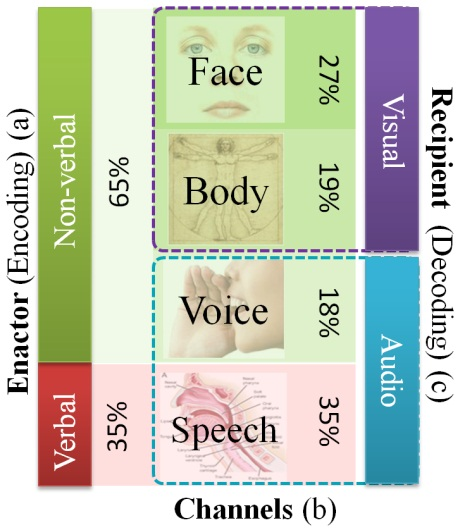
\includegraphics[width=3in]{NVCEncodings.jpg}
\end{center}
\caption{Relative importance of a) verbal vs. non-verbal cues, b) four channels of non-verbal cues, and c) visual vs. audio encoding and decoding of bilateral human interpersonal communicative cues.}
\label{Fig:Figure1}
\end{figure}

\subsubsection{Social Sight and Social Hearing}
Unlike speech, which is mostly under the conscious control of the user, the non-verbal communication channels are engaged from a subconscious level. Though people can increase their control on these channels through training, innately, individuals demonstrate certain inability to control their non-verbal cues. This inability to control non-verbal channels is referred to as the leakiness \cite{brown_social_1986} and humans (evolutionarily) have learnt to pick up these leaked signals during social interactions. For example, people can read very subtle body mannerisms very easily to determine the mental state of their interaction partner. Eye Gaze is a classic example of such subtle cues where interaction partners can detect interest, focus, involvement and role play, to name a few.  On this leakiness scale, it has been found that the voice is the leakiest of all channels, implying that emotions of individuals are revealed first in their voice before any of the other channels are engaged. The voice is followed by body, face and finally the verbal channel, speech. The leakiness is plotted on the abscissa of Figure \ref{Fig:Figure2} with the ordinate showing the amount of information encoded in the other three non-verbal communication channels. It can be seen that the face communicates the most amount of non-verbal cues, while the prosody (voice) is the first channel to leak emotional information.

\begin{figure}[h]
\begin{center}
 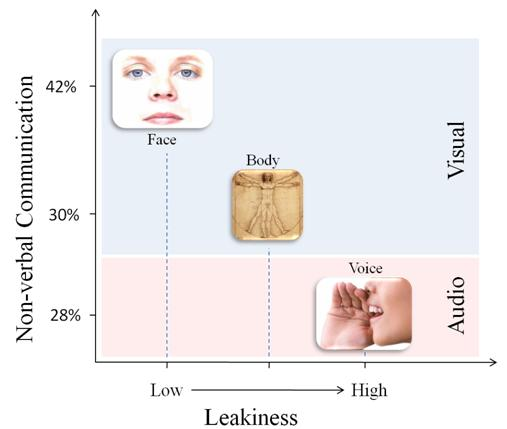
\includegraphics[width=4in]{Leakiness.jpg}
\caption{Relative communicative information plotted against its leakiness. Speech forms the verbal channel. Face, body and voice form the non-verbal communication channels.}
\label{Fig:Figure2}
\end{center}
\end{figure}

\subsubsection{Social Touch}
Apart from visual and auditory channels of social stimulation, humans increasingly rely on social touch during interpersonal interactions. For example, hand shake represents an important aspect of social communication conveying confidence, trust, dominance and other important personal and professional skills \cite{burgoon_relational_1984}. Social touch has also been studied by psychologists in the context of emotional gratification. Wetzel \cite{wetzel_midas_1984} demonstrated patron gratification effects through tipping behavior when waitresses touched their patrons. Similar studies have revealed the importance of social touch and how conscious decision making is connected deeply with the human affect system. In the recent years social touch has gained a lot of interest in the area enriching remote interactions \cite{haans_mediated_2006} \cite{bailenson_virtual_2008} to help better understand an individual's  social awareness and social presence. In the next section, we describe the term \emph{Social Situational Awareness} as seen pertinent to this report and emphasize the importance of any individual being aware of his/her social situational awareness.

\section{Social Situational Awareness}
We refer to the term Social Situational Awareness (SSA) as the ability of individuals to receive the visual, auditory and touch based non-verbal cues and respond appropriately through their voice, face and/or body (touch and gestures). Figure \ref{Fig:Figure3} represents the concept of consuming social cues and reacting accordingly to the needs of social interaction. Social cognition bridges stimulation and reciprocation and allows individuals to interpret and react to the non-verbal cues.

\begin{figure}[h]
\begin{center}
 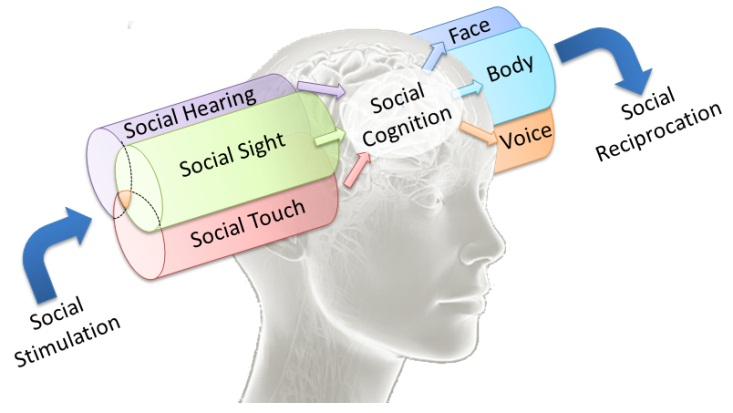
\includegraphics[width=4.5in]{SSA.jpg}
 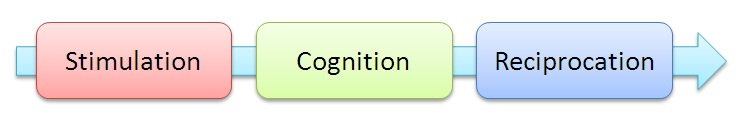
\includegraphics[width=4.5in]{SSA2.jpg}
\caption{Social Situational Awareness.}
\label{Fig:Figure3}
\end{center}
\end{figure}

The Transactional Communication Model \cite{sameroff_reproductive_1975} suggests that during any face-to-face interaction, the interpretation of the social stimulation and the corresponding social response are under the control of various factors including the culture, physical and emotional state, experience, memory, expectation, self concept and attitude of the individuals involved in the interaction. In order to effectively cognize and react to the social stimulation, it is necessary that individuals be able to receive and synthesize these above factors. Enriching social situational awareness then represents the ability of a mediator (telecommunication technology for remote interactions; social assistive technologies for the disabled population) to allow the social cognition of an individual to have access to the above mentioned factors and thereby evoking appropriate social reciprocation.

\subsection{Social Situational Awareness in Everyday Social Interactions}
\subsubsection{SSA in Dyadic Interactions}
Human communication theories have studied dyadic or bilateral interaction between individuals as the basis of most communication models. Theories of leadership, conflict and trust base their findings on dyadic interaction primitives where the importance of the various non-verbal cues is heightened due to the one-on-one nature of dyadic interactions. Eye contact, head gestures (nod and shake), body posture (conveying dominance or submissiveness), social touch (hand shake, shoulder pat, hug, etc.), facial expressions and mannerisms (smile, surprise, inquiry, etc.), eye gestures (threatened gaze, inquisitive gaze, etc.) are some of the parameters that are studied closely in dyadic understanding of human bilateral communication \cite{altmann_analysis_2007}. Enriching SSA in dyadic communication thus focuses on appropriate extraction and delivery of communicator's face, body and voice based behaviors to a remote participant or to a person who is disabled.

\subsubsection{SSA in Group Interactions}
Group dynamics refer to the interactions between members of a team assembled together for a common purpose. For example, teams of medical professionals operating on a patient, a professional team meeting for achieving a certain goal, a congressional meeting on regulations, etc. represent groups of individuals with a shared mental model of what needs to be accomplished. Within such groups, communication behaviors play a vital role in determining the dynamics and outcome of the meeting. Zancanaro et. al. \cite{zancanaro_automatic_2006} and Dong et. al.  \cite{dong_using_2007} presented one model of identifying role-play of participants in a group discussion. They identified two distinct categories of roles for the individuals within the group, namely, the socio-emotion roles and the task roles. The socio-emotional roles included the protagonist, attacker, supporter and neutral, and the task roles included the orienteer, seeker, follower and giver. These roles were dependent heavily on the emotional state (affect) of the individuals participating in the group interaction. Good teams are those where individual team members and their leaders are able to compose and coordinate their affect towards a smooth and conflict free group interaction. And effective leaders are those who can read the affect of their group member, make decisions on individual's roles and steer the group towards effective and successful decisions. Inability to access the affective cues of team members has significant consequences to team leaders leading to unresolved conflict situations and underproductive meetings, or in the worst case, the death of a patient. Thus, enriching SSA in group settings correspond to the extraction and delivery of team's interaction dynamics (which are in turn modulated in their mutual and group affect) to a remotely located team member or to a co-located individual who is disabled.

In essence, SSA enrichment technologies provide for a richer interaction experience for individuals involved either in a dyadic or group interaction. It is well established that in teams comprising of good communication strategies a shared mental model towards effective decision is achieved faster with little or no emotional stress on the team members. The lack of social awareness can lead to interactions where individuals are not committed cognitively and find it very difficult to focus their attention on the communication. This is true in the case of remote interactions, disability and situations where doctors, nurses and other medical professionals are operating simultaneously on a patient.

\subsection{Learning Social Awareness}
Figure \ref{Fig:Figure3} represents a simple unidirectional model of social stimulation and reciprocation. In reality, social awareness is a continuous feedback learning system where individuals are learning through observing, predicting, enacting and correcting themselves. It is this learning mechanism that allows people to adapt easily from one culture to another with ease - here we refer to term culture in very broadly encompassing work culture, social culture in a new environment and culture of a new team, etc. Figure \ref{Fig:Figure4} shows the continuous feedback loop involved in social learning systems, based on the model of human cognition as proposed by Hawkins \cite{hawkins_intelligence_2004}.

\begin{figure}[h]
\begin{center}
 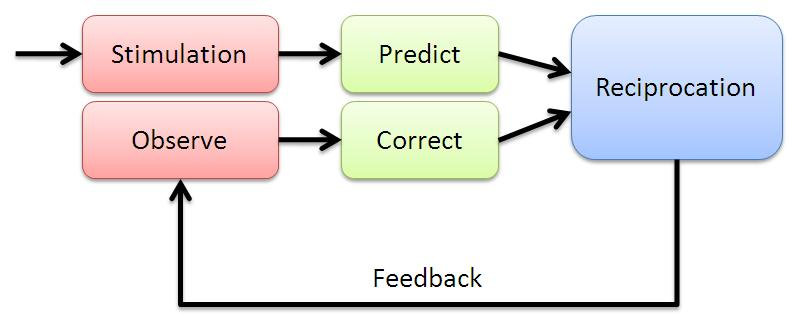
\includegraphics[width=4.5in]{SSALearning.jpg}
\caption{Social learning systems with continuous learning feedback loop.}
\label{Fig:Figure4}
\end{center}
\end{figure}

People exposed to everyday social interactions learn social skills from the three different social stimulations (social sight, social hearing and social touch) effortlessly. When faced with a new environment, individuals exercise their learned social skills to predict what social actions are appropriate in the setting. Once executed, they observe and assess their counterparts to determine if their new behavior is appropriate or not for the new setting. Such learning continues until their social rule set adapts to the new environment. Psychologists have been studying the nature of learning that happens in individuals who move from Western to Eastern cultures and vice versa. Largely, USA and Japan have been the countries of choice based on their economic equality and cultural diversity \cite{rogers_edward_2002}. In the West, large body movements and excitement in the voice are considered to be typical and to a large part encouraged as a good social skill. Similar attitudes in the East are considered to be inappropriate in professional settings and to a large extent considered indecent. An individual displaying any such inappropriate mannerisms or gestures will receive social feedback from his counterparts (everyone staring at the individual, reduced interaction with the individual, etc.).  Thus, social awareness is a learned set of rules about the environment within which the individual is present and this requires continuous monitoring of the various social channels of stimulation. Deprivation of any one of these channels can in turn affect the ability of the individual to learn social actions and responses that are pertinent to a social situation. Thus, enriching SSA not only offers the means for individuals to make appropriate social decisions, but also cognitively trains them towards effective social judgments.

-------------------------------------
In this paper, we advocate that the social separation induced by remote interactions in physically separated partners is similar to the social separation resulting from information impoverishment induced by sensory/physical disabilities in co-located interaction partners and propose technologies targeted at enriching social interactions.
--------------------------------------

\section{Components of Non-verbal Communication}
Non-verbal communications are inherently complex in nature. In order to understand the nature of these cues, psychologists have been studying these cues under three subdivisions based on what affects individual’s non-verbal cueing \cite{knapp_nonverbal_1996}. These subdivisions include,
\begin{enumerate}[(a)]
\item The communication environment
\item  The physical characteristics of the communicators
\item The behaviors of the communicators
\end{enumerate}
Below, these three items are discussed in detail providing a highlevel discussion on the nature of their influence on the non-verbal communication between individuals.

\subsection{The Communication Environment}
The communication environment or surroundings where the interactions are taking place make a huge difference of how humans respond or react \cite{hargie_social_1994} \cite{walsh_person-environment_2000}. For example, lengthy periods of extreme heat \cite{kenrick_ambient_1986} are known to increase discomfort, irritability, reduced work output and unfavorable evaluations of other. Along with the interaction partners, the environment either reinforces or depreciates the emotional experience of an individual. For example, wide open spaces and natural environments are known to be conducive for psychological stability \cite{krupat_people_1985}. Though the environmental factors just perceptual, they impose a lot of control on how humans react towards them. Some of the important environmental factors that affect interpersonal communication and non-verbal cueing are shown in the Table \ref{Tab:Tabel1}. **These are some of the well identified factors towards which psychologists and sociologists are working towards.**

\begin{table}[hpdf]
\begin{center}
\caption{The various factors of the communicator's environment that can affect interpersonal communication.}
\label{Tab:Tabel1}
\begin{tabular}{|l|l|}
\hline
\multicolumn{2}{|c|}{The Communication Environment} \\
\hline
Familiarity of the environment & \cite{sommer_personal_1969} \cite{sommer_tight_1974} \\
Colors in the environment & \cite{schauss_psysiological_1985} \cite{bottomley_interactive_2006} \\
Other people in the environment	& See next two subsections. \\
Architectural Designs & \cite{farrenkopf_university_1980} \\
Objects in the environment & \cite{moos_human_1985} \\
Sounds  & \cite{manusov_attribution_2001} \cite{north_-store_1997} \\
Lighting & \cite{meer_light_1985} \\
Temperature & \cite{kenrick_ambient_1986} \\
\hline
\end{tabular}
\end{center}
\end{table}

\subsection{The Physical Characteristics of the communicators}
The physical appearance of a person is very important aspect of non-verbal cueing. People draw impressions of their communication partner as soon as they see them. The human body acts like means for communicating important sociological parameters like status, interest, dominance etc. Researchers have found cultural and global preferences in overall body image and any deviations from the norm affects interactions between people. For example, facial babyishness \cite{berry_attractive_1991} has been found affect judgment of facial attractiveness, honesty, warmth and sincerity. Any deviation from the babyishness has been correlated to immediate reduction in the judgment of these traits. A similar such example is the clothing that people wear. It has been found that first impressions are positive if the interviewer and interviewee are clothed similarly \cite{johnson_clothing_1977}. Table \ref{Tab:Table2} shows the important aspects of a person's physical appearance that affects the interpersonal interaction. Various psychological studies have been conducted towards understanding the model of human perception of character. Very little is known on the reasons for some of the human norms, but it is an active area of research that is being explored rigorously, especially, in the context of group behaviors and personal mannerisms with work environments \cite{helen_h._jennings_sociometry_1959}.

\begin{table}[hpdf]
\begin{center}
\caption{The physical characteristics of a communicator that can affect interpersonal communications.}
\label{Tab:Table2}
\begin{tabular}{||l||l||}
\hline
\hline
\multicolumn{2}{||c||}{The Physical Characteristics} \\
\hline
\hline
The human facial attractiveness	& \cite{berry_attractive_1991} \cite{zebrowitz_reading_1997} \cite{berry_perceiving_1986}\\
\hline
Body shape & \cite{cortes_physique_1965} \cite{tucker_physical_1984}\\
\hline
Height of a person & \cite{cameron_courtship_1977}\\
\hline
Self image & \cite{ogden_prevalence_2002}\\
\hline
Body color & \cite{griffin_black_1996}\\
\hline
Body smell & \cite{porter_olfaction_1998} \cite{lord_identification_1989} \cite{russell_human_1976}\\
\hline
Body hair & \cite{barber_mustache_2001}\\
\hline
Clothing & \cite{johnson_clothing_1977} \cite{hensley_effects_1981}\\
\hline
Personality	& \cite{joseph_uniforms_1986} \cite{rosenfeld_clothing_1977}\\
\hline
Body decoration or artifacts & \cite{sanders_customizing_2008}\\
\hline
\hline
\end{tabular}
\end{center}
\end{table}

\subsection{Physical Characteristics that affect interpersonal communication}
\subsubsection{Behavior of the Communicator}
The last of the three units of non-verbal communication is the behavior of the communicators. While the term behavior is used loosely in defining this unit, this encompasses both static posture and dynamic movements demonstrated by communicators. Of the three units of non-verbal communication, the behavior forms the most important aspect. Most part of the emotional information encoded by humans is delivered through the behavior of individuals during social interactions. Gestures, Posture, Touch and Voice form the basic subdivisions in behavioral non-verbal cueing. While the entire human body is important for the communication of these cues, the face and eyes play a major role.

\subsubsection{Gesture}
Gestures are dynamic movement of face and limbs displayed during interpersonal communication. Together, they convey a lot of information that is sometimes redundant (with speech) while other times deliver emotional information about the enactor. Most often gestures are classified based on their occurrence with speech. Accordingly, there are
\begin{enumerate} [(a)]
\item Speech-independent gestures, or emblems (like shrug, thumbs up, victory sign etc), that are mostly visual in nature and convey the user's response to the situation \cite{ekman_nonverbal_1976} \cite{wagner_field_2003}.
\item Speech-related gestures, or illustrators (pointing to a thing, drawing a shape while describing etc) \cite{efron_gesture_1972}.
\item Punctuation gestures, that emphasize, organize and accent important segments of a communication, like pounding the hand, raising a fist in the air etc.
    \end{enumerate}

\subsubsection{Posture}
Posture refers to the temporary limb and body positions assumed by individuals during interpersonal interactions.  Posture is a very effective medium for communicating some of the important non-verbal cues like leadership, dominance \cite{weisfeld_erectness_1982}, submissiveness and social hierarchy \cite{grant_comparison_1963}. For example, people who show a tendency of dominance tend to extend their limbs out while sitting thereby displaying an overall larger body size. Similarly, submissiveness seems to be correlated to reducing the overall body size by keeps the limbs together.

Both gestures and postures are influenced heavily by the cultural background of the individual and also varied with the geographical location \cite{kleinsmith_cross-cultural_2006}. Though the cultural influence if true with other non-verbal and verbal cues, the perceived difference is the highest in gestures and posture displayed by individuals.

\subsubsection{Touch}
Social touch has been a very important aspect of non-verbal communication in humans. Developmental biologists believe that the first set of sensory responses in a human fetus is touch \cite{montagu_touching:_1986}. From a social context this sensory channel is very well used in conveying important interpersonal cues such as interest, intimacy, warmth, confidence, leadership and sympathy \cite{afifi_use_1999}. Touch is a powerful means of unconscious interaction and it is believed that people who are very good in their social skills rely upon touch a lot \cite{hertenstein_communicative_2006}. Historically, the sense of touch (Haptics Communication \cite{hertenstein_touch_2006}) has been studied by psychologists in the perspective of understanding the human sensory system, but recently, haptics has grown out into the technology front providing human machine interfaces that augment or replace visual and auditory interfaces \cite{robles-de-la-torre_principles_2008}.

\subsubsection{Face}
The face is the primary channel for non-verbal communication. Humans are efficient in conveying and receiving plethora of information through subtle movements of their face and head. This focus on the face develops from a very young age and it has been shown that by 2 months, infants are adept in understanding facial gestures and mannerisms \cite{carver_development_2002}. The human face has very fine muscular control allowing it to perform complex patterns that are common to humans, while at the same time being vastly individual \cite{rinn_neuropsychology_1984}. The facial appearance of an individual is due to their genetic makeup, transient moods that stimulate the facial muscles and due to chronically held expressions that seem to set in and become permanent. Human visual system has developed the ability to read these subtleties on people's faces and interpret all the three aspects of the face - genetic makeup (person's identity through face recognition), transient mood (facial expression and emotion recognition), and permanent expression on the face (default neutral face of individuals). While the aspects of permanent facial appearance are important in the recognition of the individual, from a non-verbal communication perspective, the primary function of the face is directed towards communicating emotions and expressions.

The understanding of the human facial expression space was immensely increased by the work of Ekman, Frisen \cite{ekman_facial_1978} and Izard \cite{izard_maximally_1983} in the late 1970s. They independently measured precise facial movement patterns and correlated these individual movements with facial expressions on the human face. While Izard developed these patterns on infants, the Facial Action Coding System (FACS) developed by Ekman and Frisen has become the de facto standard for measuring facial expressions and emotions. FACS allow expression and emotion researchers to encode facial movements into accurate contraction and relaxation of facial muscles. Based on these facial actions, Ekman and Frisen discovered the global occurrence of seven basic judged emotions. As psychologists have started to master the FACS system of analyzing facial actions, human computer interaction specialists have started to use the same FACS encodings for building better interfaces that can determine human affect and respond accordingly.

\emph{Facial Action Coding System (FACS):}
FACS defines all possible facial feature movements into Action Units (AU) which represent movement of facial features (like lips, eye brow, chin etc). The AUs are the net effect of facial muscle contraction and relaxation, though they are not directly related to the muscles. Table below shows the different AUs that form the basis of FACS based facial coding with the appropriate number and the associated facial feature movement.

\begin{table}[hpdf]
\begin{center}
\caption{FACS communicative actions on the human face}
\label{Tab:Table2}
\begin{tabular}{|l|l||l|l|}
\hline
1 & Inner Brow Raiser & 24 & Lip Pressor\\
2 & Outer Brow Raiser & 25 & Lips part\\
4 & Brow Lowerer & 26 & Jaw Drop\\
5 & Upper Lid Raiser & 27 & Mouth Stretch \\
6 & Cheek Raiser & 28 & Lip Suck\\
7 & Lid Tightener & 29 & Jaw Thrust \\
9 & Nose Wrinkler & 30 & Jaw Sideways \\
10 & Upper Lip Raiser & 31 & Jaw Clencher\\
11 & Nasolabial Deepener & 32 & Lip Bite \\
12 & Lip Corner Puller & 33 & Cheek Blow \\
13 & Cheek Puffer & 34 & Cheek Puff \\
14 & Dimpler & 35 & Cheek Suck \\
15 & Lip Corner Depressor & 36 & Tongue Bulge \\
16 & Lower Lip Depressor & 37 & Lip Wipe\\
17 & Chin Raiser & 38 & Nostril Dilator \\
18 & Lip Puckerer & 39 & Nostril Compressor\\
19 & Tongue Out & 41 & Lid Droop \\
20 & Lip stretcher & 42 & Slit\\
21 & Neck Tightener & 43 & Eyes Closed\\
22 & Lip Funneler & 44 & Squint\\
23 & Lip Tightener & 45 & Blink\\
& & 46 & Wink\\
\hline
\end{tabular}
\end{center}
\end{table}

\subsubsection{Eye}
Like the human face, eyes are very important for the control of non-verbal communication. This involvement of human eyes comes from the functions that gaze and mutual gaze play in everyday human interpersonal communication \cite{argyle_gaze_1976}. People use their gaze to convey subtle information that enables smooth verbal interaction which eventually leads to information exchange \cite{kleinke_gaze_1986}. From a research perspective, the function of gaze has been classified into four important functional categories \cite{kendon_functions_1967}. These include

\begin{table}[hpdf]
\begin{center}
\caption{The role of human eye in interpersonal communications.}
\label{Tab:Table4}
\begin{tabularx}{5.5in}{|X|X|}
\hline
Regulating the flow of communication & One of the most important functions of gaze is the regulation of verbal communication in bilateral and group communications. People use gaze to shift focus, bring the attention of a group of people to one thing, turn taking in group conversations \cite{mast_dominance_2002} and eliciting response from communication partners \cite{bavelas_listener_2002}. \\
\hline
Monitoring feedback & Gaze provides a means for individuals to get feedback during conversations and communications. Feedback is a very important tool while people converse. Humans study the eyes of the listener to cognitively inject or eliminate more verbal information into the conversation \cite{van_dulmen_shifts_1997}. \\
\hline
Reflective of cognitive activity & Both listeners and speakers tend not to gaze at others when they are processing complex ideas or tasks. Studies have shown that people can answer better when they close their eyes and are allowed to process their thoughts \cite{glenberg_averting_1998}. Thus, cognitive processing is displayed very elegantly by monitoring eye gaze patterns. \\
\hline
Expressing emotions & Along with the facial muscular movements, the eyes play a vital role in the expression of emotions. In fact, in human computer interaction research, it has been found that relying on the eyes and the eyelids alone can provide more accurate delivery of affect information when compared to the entire face \cite{orozco_confidence_2008}. Verbal communication tends to move the lips and mouth quickly and randomly that can make image and video processing of expressions very tough. Some of the more recent spontaneous expression recognition research is focusing on the eyes for this very reason. \\
\hline
\end{tabularx}
\end{center}
\end{table}



\chapter{MOTIVATION}
\DoubleSpacing
\setlength{\parindent}{.5in}
In this chapter we discuss three important problems that highlight the need to communicate social situational awareness to individuals involved in interpersonal interactions.

\section{Assistive Technology}
most part of the non-verbal encoding happens through visual media. While some parts of these cues are delivered along with speech, most part of the nonverbal communication is inaccessible to someone with visual impairment or blindness. This disconnect from the visual stimulations deprive the individuals of vital communicative cues that enrich the experience of social interactions.  People who are blind cannot independently access this visual information, putting them at a disadvantage in daily social encounters.  For example, during a group conversation it is common for a question to be directed to an individual without using his or her name-instead, the gaze of the questioner indicates to whom the question is directed. In such situations, people who are blind find it difficult to know when to speak because they cannot determine the direction of the questioner's gaze. Consequently, individuals who are blind might be slow to respond or talk out of turn, possibly interrupting the conversation. As another example, consider that people who are blind cannot use visual cues to determine when their conversation partners change positions (e.g., pacing the floor or moving to a more comfortable chair). In this scenario, an individual who is blind might inadvertently create a socially awkward situation by speaking in the wrong direction.

To compound these problems, sighted individuals are often unaware of their non-verbal cues and often do not (or cannot) make appropriate adjustments when communicating with people who are blind. Also, people who are blind often do not feel comfortable asking others to interpret non-verbal information during social encounters because they do not want to burden friends and family.  The combination of all these factors can lead people who are blind to become socially isolated \cite{segrin_poor_2000}, which is a major concern given the importance of social interaction. While people who are blind and visually impaired face a difficulty in social interactions, research in rehabilitation training for these populations recommends that the social involvement for these individuals have to substantially increase in order to enable their acceptance of the society.

National Center for Health Statistics reported in $2007$ that the estimated number of visually impaired and blind people totals up to $21.2$ million in the United States alone . Global numbers are daunting. In $2002$ more than $161$ million people were visually impaired, of whom $124$ million people had low vision and $37$ million were blind . World Health Organization reports that more than $82$\% of the populations who are blind or visually impaired are of age $50$ or older. With the life expectancy going up in most developing countries, the percentage of general population entering into some sort of visual impairment is going to increase in the coming years.

Recently, Jindal-Snape \cite{jindal-snape_generalization_2004} \cite{jindal-snape_use_2005} \cite{jindal-snape_using_1998} carried out extensive research in understanding social skill development in the blind and visually impaired. She has studied individual children (who are blind) from India where the socio-economic conditions do not provide for trained professionals to work with children with disabilities. Her seminal work in understanding social needs of children who are blind have revealed two important aspects of visual impairment that restricts seamless social interactions.

While most persons who are blind or visually impaired eventually make accommodations for the lack of visual information, and lead a healthy personal and professional life, the path towards learning effective accommodations could be positively effected through the use of assistive aids. Specifically, children with visual disabilities find it very difficult to learn social skills while growing amongst sighted peers, leading to social isolation and psychological problems \cite{jindal-snape_generalization_2004}. Social disconnect due to visual disability has also been observed at the college level \cite{shinohara_blind_2009} where students start to learn professional skills and independent living skills. Any assistive technology aid that can enrich interpersonal social interactions could prove beneficial for persons who are visual disabled.

\section{Remote Interactions}
An industry survey \cite{solomon_challenges_2010} of $1592$ individuals who collaborated remotely, carried out by RW3 CultureWizard - a company focused on improving international collaborations - reported difficulties similar to what was faced by the individuals who are blind. "Respondents found virtual teams more challenging than face-to-face teams in managing conflict ($73$\%), making decisions ($69$\%), and expressing opinions ($64$\%). The top five challenges faced during virtual team meetings were insufficient time to build relationships ($90$\%), speed of decision making ($80$\%), different leadership styles ($77$\%), method of decision making ($76$\%), and colleagues who do not participate ($75$\%)." These results can be correlated to the need for Social Situational Awareness in group settings, specifically one that can promote leadership and personal understanding of each other as indicated in Section 2.1.2.

Further, when the participants were asked about the personal challenges faced during virtual team meetings, they reported inability to read non-verbal cues ($94$\%), absence of collegiality ($85$\%), difficulty establishing rapport and trust ($81$\%), difficulty seeing the whole picture ($77$\%), reliance on email and telephone ($68$\%), and a sense of isolation ($66$\%)." Delivering non-verbal cues, establishing trust and rapport, and easing isolation are all derivatives of increasing one's social connection to their interaction partners, be it remote or face-to-face. Observing people who are disabled and the way they communicate with their co-located partners, it is possible to derive inspirations for novel social mediation technologies. The following subsection discusses one example of how to develop an evidence-based social situational awareness model based on hand shaking in the blind population as an example of social interaction between participants.

\begin{table}
\caption{Survey on the challenges of remote interaction \cite{solomon_challenges_2010}}
\label{Table:Tab3}
\begin{tabular}{|l|}
\hline
Challenges in virtual teams compared to face-to-face teams \\
\hline
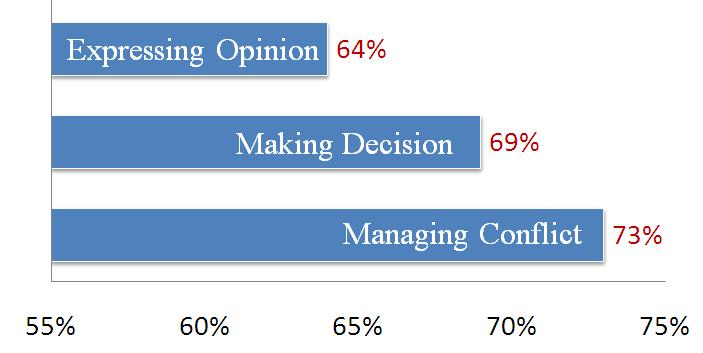
\includegraphics[width=3in]{Suggestion1.jpg}\\
\hline
Top five challenges faced during virtual team meetings \\
\hline
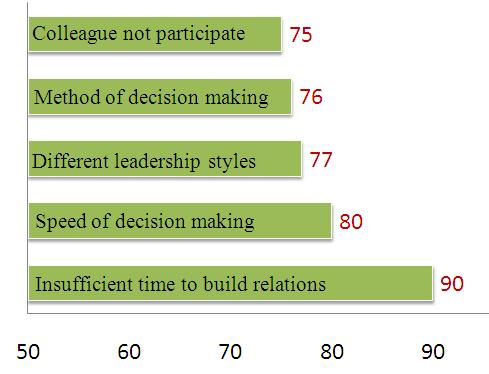
\includegraphics[width=3in]{Suggestion2.jpg}\\
\hline
Personal challenges during virtual team meetings\\
\hline
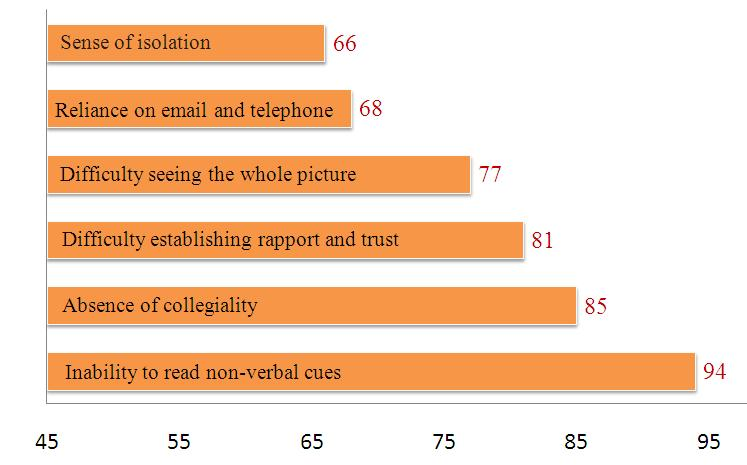
\includegraphics[width=4.5in]{Suggestion3.jpg}\\
\hline
\end{tabular}
\end{table}

\section{Medical Teams}
Modern day critical care facilities require multi-disciplinary medical professionals to operate on a single patient, all at the same time. This imposes an hard and fast requirement on the professionals to work as a team. Unlike typical professional teams who choose their members over thorough deliberation, medical teams assume shape dynamically based on whichever medical professional is available on the hospital floor at the time of emergency. Further, these teams last for a very short duration of time (the duration dictated by the emergency) and new teams will form dynamically per need basis. Studies show that teams that establish well articulated communication between members perform well  under the stressful environment. Unfortunately, this is not true of all medical teams and one individual's stress may very well propagate through the team and breakdown mutual communication and support, leading to patient's death.

\begin{figure}
\centering
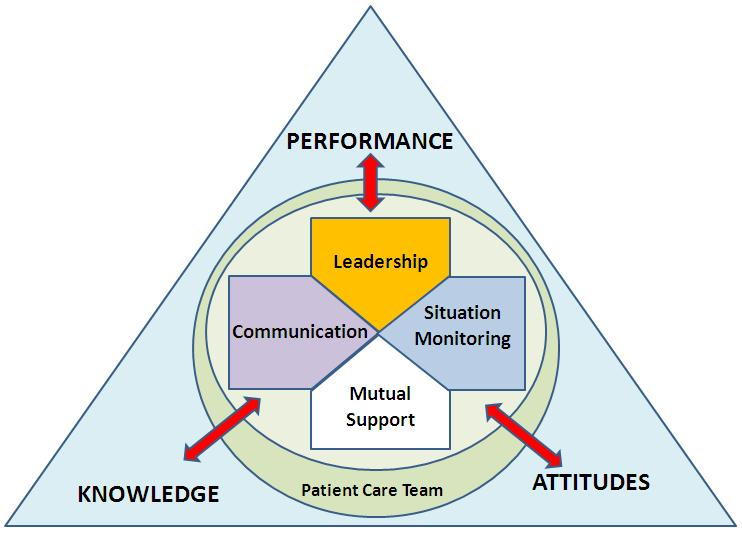
\includegraphics[width=4in]{TeamStepps.jpg}
\caption{\textbf{TeamSTEPPS:} Team Strategies and Tools to Enhance Performance and Patient Safety}
\label{fig_cp}
\end{figure}

The importance of studying a group of physicians entering a medical situation as a single operating unit began to appear in the focus of behavioral scientists with the publication of the Institute of Medicine (IoM) report titled \emph{To Err is Human: Building a Safer Health System} in Dec 1999. One of the four core messages from the report identified that patient life is lost not because of the failure of an individual, but due to the failure of the group as a whole. Since this report, Agency for Healthcare Research and Quality (AHRQ) and Department of Defense (DoD) have focused on the team failure from an Evidence-Based Medicine perspective and released Team Strategies and Tools to Enhance Performance and Patient Safety (TeamSTEPPS) [13] as the standard for team training in health care. The core of TeamSTEPPS focuses on the need to have (a) leadership, (b) mutual support, (c) communication, and (d) situation monitoring (or a shared mental model) among the team members.

As seen from Figure 1, the skills component TeamSTEPPS focuses on the individual physician and the team's ability to work together as a system. Leadership, Communication, Situation Monitoring and Mutual Support were all derived from earlier DoD and AHRQ lead studies in medical team management and are based on the underlying principles of: Team Leadership [8], Mutual Performance Monitoring [9], Backup Behavior [10], Adaptability [11], Team/Collective Orientation [12], Shared Mental Model [13] [11], Mutual Trust [14] and Closed loop Communication [10]. For a detailed analysis of each of these principles, please see King et. al. [4]. Most of these principles are in turn derivatives of the social skill set of the individuals who make up the medical team that is responsible for the patient safety. It have been shown that in cases of medical errors, leading to loss of life, communication breakdown between one or more team members resulted in an avalanche of problems eventually resulting in death.

The four team performance qualities identified above depends intricately on each medical personnel's communication abilities.  Behavioral psychologists have been studying the impact of socio-emotional states, especially stress induced socio-emotional states, on the performance of professionals and conclude that the direct artifact of stress include deprecated decision making, failure in leadership and breakdown of mutual support. Assessing the socio-emotional and communication skills of the professionals within the critical care unit will provide an unfettered advantage towards determining metrics of team performance under stress. To this end, in this paper we propose an initial set of three parameters that need to be studied towards advancing patient safety in critical care environments. Note that these research questions are still under investigation and their efficacy can only be hypothesized based on preliminary socio-behavioral studies conducted in related areas, under laboratory conditions.

\subsection{Evidence for Group Performance and Leadership}
\subsubsection{Group Dynamics}
As the term implies GD focuses on studying the various components of group communication, including inter-agent communication [19], productivity of a given group [20], level of understanding of each other's potentials and limitations, job satisfaction and combined creativity of a team [21]  to name a few. In the recent years, the interest in understanding group dynamics in work environments has tremendously increased in interdisciplinary teams involving computer scientists and socio-behavioral psychologists in the area of Computer Supported Collaborative Work (CSCW) [22]. In the context of medical teams, group dynamics focuses on the ability of the physicians/specialists to intercommunicate their needs. During emergency situations, group dynamics facilitates the emerging Shared Mental Model [23].

In the classical model for group dynamics, Bruce Tuckman [24], defines four stages in the formation of an efficient group. Forming, Storming, Norming and Performing describe the typical process that the groups go through before delivering at their best. The stages of Storming and Norming are deeply connected to the individual group member's abilities to communicate, coordinate and emphasize with their fellow group members. The socio-emotional interactions between the group members dictate how quickly or slowly a group will progress from the formative first stage to performing fourth stage [25]. If every individual group member can be assessed on their socio-emotional interactions - in general with everyone and in specific with professional teams - it is possible to determine what teams will work better together and progress through the four stages quickly towards efficient group performance.

\subsubsection{Leadership}
Theories of leadership have proposed evidence-based models for explaining qualities exemplified in successful leaders. From bureaucratic leaders to political leaders, the models described to explain the qualities of leaders vary dramatically. There is no single accepted definition of what a leader should represent, as the problem of identifying a leader is highly contextual in nature. Recently, the functional model of leadership has been developed to describe team leaders as having self regulation which translates to learning, performance and adaptability. These models allow studying of dynamic teams that are formed in very short durations (like medical response teams) and allow monitoring of each individual and their contribution to the group activity [26]. Kozlowski et. al. have described a dynamic multi-goal model for team leadership as shown in Figure 3. Accordingly, they describe effective leaders as those who can not only assess simultaneously their own goals while keeping track of team goals while approaching a dynamically evolving situation.

\begin{figure}
\centering
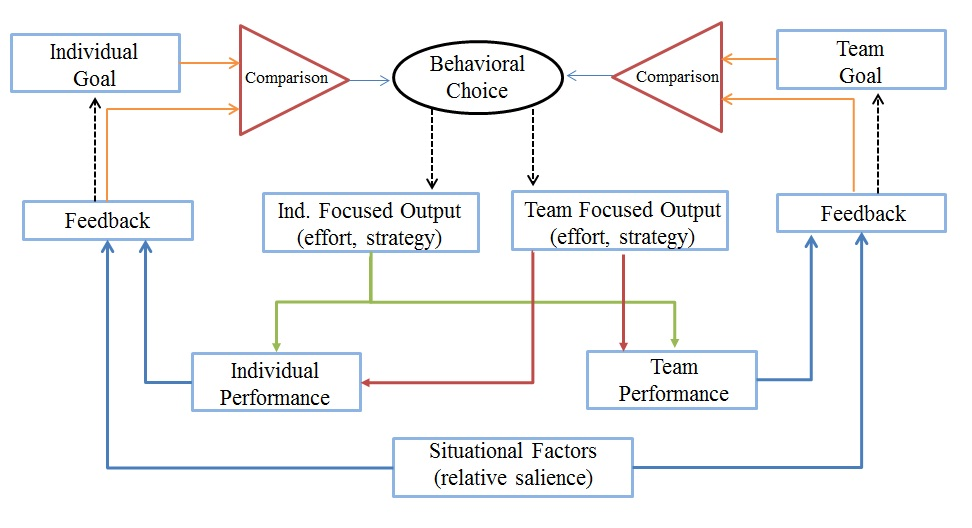
\includegraphics[width=5in]{Leadership.jpg}
\caption{Multi goal model of self regulation for effective team regulation.}
\label{fig_cp}
\end{figure}


While Figure 3 shows the behavioral choice of the leader to be a vital component of self regulation and team regulation, very little work has been focused on studying the effect of leader affect on team dynamics. Recently Sy et. al. [27] have demonstrated how important it is for the leader to control and regulate his/her affect cues within dynamical formed teams. The mood of the leader percolates through the team and can have net positive or negative effect on the team outlook and performance. The dynamic nature of team formation is further complicated in medical teams as the responsibility shifts very quickly from one specialist to another as they operate on the patient [28]. Socio-emotional role play of leaders in such dynamic teams is vital to the execution of the current task and smooth development of the shared mental model.

\vspace{-0.1in}
\subsection{Human Communication Challenges in Medical Teams}
\subsubsection{Automated monitoring of group dynamics to determine communication breakdowns}
\vspace{-0.13in}
Current team performance analysis systems are mostly based on retrospective video stream analysis collected during simulations of hospital emergency codes. The analyses are mostly based on expert's opinion of what happened during critical incidents of the simulation [6] [3]. Unfortunately, expert's time is very valuable and post-simulation analysis may not get sufficient attention due to increased hospital load. For long, researchers have questioned how communication between medical team members vary over the period of the emergency code execution [2], but very little is understood on the basics of the communication patterns during emergency, mostly due to the lack of automated annotation system that does not require expensive specialist time. Automated team performance analysis systems that focus on detecting specific instances of communication breakdown occurring during code simulation could greatly enhance our understanding of team work and how it can be enhanced through training.

\vspace{-0.1in}
\subsubsection{Automatic evaluation of the social affinity between team members}
\vspace{-0.13in}
Sociograms (social affinity maps) have been used historically to determine the interpersonal match between members of a team or an organization. Sociograms are obtained through the process of sociometry [15], which quantitatively measures the relationships of individuals who exist within a social space. As mentioned earlier, in medical teams, the social space happens to be the emergency room where the team assembles with very little or no time to assess who are the members of the team. Sociometry is achieved through a set of evaluations that can assess the social interactions between individuals. The measurements could happen within the environment where the individuals interact (the medical team) or outside (casual interactions). Technologies developed to assess sociometric affinity between professionals could in turn provide quantitative evaluations of the social interactions between individuals. Sociograms developed at a hospital level could offer effective tools for quick team formations. Teams formed out of specialists, technicians and nurses who are closer to one another on the sociogram could offer a team with relatively less emotional stress. Socially closer individuals will also exhibit better communication, thereby increasing team performance.

\vspace{-0.1in}
\subsubsection{Leadership evaluation and nomination through long term monitoring of individuals}
\vspace{-0.13in}
Theories of leadership have proposed evidence-based models for explaining qualities exemplified in successful leaders. Recently, the functional model of leadership [7] has been developed to describe team leaders as having self regulation which translates to learning, performance and adaptability. These models allow studying of dynamic teams that are formed in very short durations (like medical response teams) and allow monitoring of each individual and their contribution to the group activity.Reference [7] also describes a dynamic multi-goal model for team leadership which models effective leaders as those who can not only assess their own goals but also keep track of team goals, while approaching a dynamically evolving situation. Technologies developed towards understanding and modeling human interactions and communications can provide the tools needed to measure leadership qualities through long term monitoring.






\chapter{ASSISTIVE TECHNOLOGY DESIGN}
\DoubleSpacing
\setlength{\parindent}{.5in}
Affective Computing research has employed algorithmic framework to quantitatively study both verbal and non-verbal cues displayed by the humans during social communication.  Signal streams from various sensors, including visual sensors (e.g. cameras), audio sensors (e.g. microphones) and various physiological sensors (such as EEG, EMG, and galvanic skin resistance sensors) have been used to evaluate human emotional states.  A good review of research work in Affective Computing can be found in \cite{zhihong_zeng_survey_2009}.  This research has enabled a better understanding of human physiological signals, with respect to emotional states, and the results have been used to facilitate human-computer interaction (HCI). In theory, a system that can detect non-verbal social cues could also be used as an assistive device to provide social feedback to people with disabilities.  The emphasis here would not be so much on interpreting these cues as on presenting social cue information to the user, and allowing the user to interpret them.  However, very little research has been done towards finding intuitive methods for presenting social cue information to humans.  \cite{ur_rehman_manifold_2007} developed a haptic chair for presenting facial expression information.  It was equipped with vibrotactile actuators on the back of the chair that represented some specific facial feature. Experiments conducted by the researchers showed that people were able to distinguish between six basic emotions.  However, this solution had the obvious limitation that the user needed to be sitting in the chair to use the system.

\emph{Observation 1: Assistive technology designed towards social assistance should be portable and wearable so that the users can use them at various social circumstances without any restriction to their everyday life.}

People with disabilities are not always able to perceive or interpret implicit social feedback as a guide to improving their communication competence.  However, they might be able to use explicit feedback provided by a technological device.  Rana and Picard \cite{teeters_self-cam:_2006} developed a device called Self Cam, which provides explicit feedback to people with Autism Spectrum Disorder (ASD).  The system employs a wearable, self-directed camera that is supported on the users own shoulder to capture the user's facial expressions. The system attempts to categorize the facial expressions of the user during social interactions to evaluate the social interaction performance of the ASD user.  Unfortunately, the technology does not take into account the social implication of assistive technologies. Since the technology is being developed to address social interactions, it is important to take into account the social artifacts of technology. A device that has unnatural extensions could become more of a social distraction for both the participants and users than as an aid.


\emph{Observation 2: Assistive technology designed towards social assistance should allow seamless and discrete embodiment of sensors or actuators making sure the device does not become a social distraction.}

Vinciarelli et. al. \cite{vinciarelli_social_2008} have described the use of discrete technologies for understanding social interactions within groups, specifically targeting professional environments where individuals take decisions as a group. They analyze the use of bodily mannerisms and prosody to extract nonverbal cues that allow group dynamics analysis. They rely on simple sensors in the form of wearable tags \cite{kim_meeting_2008} which detect face to face interaction events along with prosody analysis to determine turn taking, emotion of the speaker, distance to an individual etc. Pentland describes these signals captured during group interactions as \cite{pentland_honest_2008} honest signals. Some of his recent works \cite{vinciarelli_social_2008-1} in the area of social monitoring hopes to capture these signals and provide feedback to individuals about their social presence within a group. The use of social feedback is illustrated elegantly in their work but their findings relied on sensors carried by all individuals involved in the study. Having everyone in a group wear sensors has proved to be a viable and productive approach for studying group dynamics.  However, this approach is not viable as a strategy for developing an assistive technology, as it is not realistic to assume that everyone who interacts with a person with a disability will wear sensors.

\emph{Observation 3: Assistive technology designed towards social assistance should incorporate mechanisms embodied on the user to determine both self and other's social mannerism.}

In two independent experiments \cite{transon_using_1988} and \cite{felps_modification_1988}, researchers developed a social feedback device that provides intervention when a person with visual impairment starts to rock their body displaying a stereotypy. \cite{transon_using_1988} designed a device that consisted of a metal box with a mercury level switch that detects any bending actions. The feedback was provided with a tone generator that was also located inside the metal box.  The entire box was mounted on a strap that the user wears around his/her head. The authors tested it on a congenitally blind individual who had severe case of body rocking and they conclude that the use of any assistive technology is useful only temporarily while the device is in use. They state that the body rocking behavior returned to baseline levels as soon as the device was removed. Since the time of this experiment, behavioral psychology studies have explored short term feedback for rehabilitation \cite{jindal-snape_use_2005}, and these studies support the above observation that short term feedback is often detrimental to rehabilitation and subject's case invariably worsens. Unfortunately, due to the prohibitively large design of the device developed by these researchers, it was impossible to have the individual wear the device over long durations.

\emph{Observation 4: Assistive technology designed towards social assistance and behavioral rehabilitation should be used over long durations in such a way that the feedback is slowly tapered off over a significantly longer duration of time.}


In \cite{felps_modification_1988} researchers used a 'Drive Alert' (driver alerting system that monitors head droop) to detect body rocking and provide feedback to a congenitally blind 21 year old student. The research concludes that they were able to control body rocking effectively, but the device could not differentiate between body rocks from any other functional body movements. This device, primarily built to sense drooping in drivers provides no opportunity to differentiate between a body rock and a functional droop. Use of such devices could only be negative on the user as a large number of false alarms would only discourage an individual from using any assistive technology.

\emph{Observation 5: Assistive technology designed towards social assistance and behavioral rehabilitation should be effective in discriminating social stereotypic mannerisms from other functional movements to keep the motivation of device use high.}


\section{Conceptual Framework}
\subsection{Design principles for social assistive and rehabilitative devices}
A device that is developed to facilitate the social interactions of people with sensory, or cognitive disabilities might do so by, (a) detecting social cues during social interactions and delivering that information to the user in real time to enable empathy, or (b) detecting the user's stereotypic behaviors during social interactions and communicating that information to the user in real time to provide social feedback.  The first device might be classified as an assistive technology, while the second might be classified as a rehabilitative technology.  Ideally, such a device would be based on the following design principles:

\begingroup
\leftskip0.5in
\setlength{\parindent}{0in}
\emph{Design principle 1:} The device should be portable and wearable so that it can be used in any social situation, and without any restriction on the user's everyday life.

\emph{Design principle 2:} The device should employ sensors and personal signaling devices that are unobtrusive, and do not become a social distraction.

\emph{Design principle 3:} The device should include sensors that can detect the social mannerisms of both the user and other people with whom the user might communicate.

\emph{Design principle 4:} The device should be comfortable enough to be worn repeatedly for extended periods of time, to allow it to be used effectively for rehabilitation.

\emph{Design principle 5:} The device should be able to reliably distinguish between the user's problematic stereotypic mannerisms and normal functional movements, to ensure that it will be worn long enough to achieve rehabilitation.

\endgroup

\section{Requirements Analysis for a Social Assistive Technology for Individuals who are Blind and Visually Impaired}
In order to identify the unmet needs of the visually impaired community, two focus groups consisting primarily of people who are blind, as well as disability specialists and parents of students with visual impairment and blindness where conducted \footnote{ In  order  to  understand  the  assistive  technology  requirements  of  people  who  are  blind, we conducted two focus group studies (one in Tempe, Arizona USA - $9$ participants, and another in Tucson, Arizona USA - $11$ participants) which included:
\begin{enumerate}[1.]
\item Students and adult professionals who are blind,
\item Parents of individuals who are blind
\item Professionals who work in the area of blindness and visual impairments.
\end{enumerate}
There was unanimous agreement among participants that a technology that would help people with visual impairment to recognize people or hear them described would significantly enhance their social life.}. Members of these focus groups who were blind or visually impaired were encouraged to speak freely about their challenges in coping with daily living. During these focus groups, the participants agreed on many issues as being important problems. However, one particular problem - that of engaging freely with their sighted counterparts - was highlighted as a particularly important problem that was not being addressed by technology specialists \footnote{  To quote some candidate's opinion about social assistance technology in a everyday setting:
\begin{itemize}
\item \"It would be nice to walk into a room and immediately get to know who are all in front of me before they start a conversation\".
\item One young man said, \"It would be great to walk into a bar and identify beautiful women\".
\end{itemize}}.

While various other examples were cited by individuals during these focus group studies, the inability to access non-verbal cues were considered of highest priority. Based on these discussions, a list of needs was complied that characterized social needs often experienced by people with visual impairments. In doing so, two important aspects of social interaction were identified. These included
\begin{enumerate}[1.]
\item Access to the non-verbal cues of others during social interactions, and
\item How one is perceived by others during social interactions.
\end{enumerate}

These needs correlated with the psychology studies conducted by Jindal-Snape with children who were visually impaired. She identifies these two needs under the \emph{Social Learning} and \emph{Social Feedback}. While these two important categories were identified, for simplification, the non-verbal cue needs were reduced to $8$ aspects of social interactions that focused primarily on the physical characteristics of the interaction partner and the behaviors of the
interaction partner. These questions were developed with the help of visually impaired professionals and students:

\begin{enumerate}[1.]
\item Knowing how many people are standing in front you, and where each person is standing.
\item Knowing where a person is directing his/her attention.
\item Knowing the identities of the people standing in front of you.
\item Knowing something about the appearance of the people standing in front of you.
\item Knowing whether the physical appearance of a person who you know has changed since the last time you encountered him/her.
\item Knowing the facial expressions of the person standing in front of you.
\item Knowing the hand gestures and body motions of the person standing in front of you.
\item Knowing whether your personal mannerisms do not fit the behavioral norms and expectations of the sighted people with whom you will be interacting.
\end{enumerate}

Further, in order to understand the importance of these non-verbal communication primitives an online survey was carried out to determine a self-report importance map of the various non-verbal cues. This list of questions included both the importance from the perspective of allowing access to the non-verbal cues of the interaction partner (for enabling Social Learning), while also focusing on the personal body mannerism (for enabling Social Feedback) of the individual.The online survey was anonymously completed by $28$ people, of whom $16$ were blind, $9$ had low vision, and $3$ were sighted specialists in the area of visual impairment and vocational training. The online survey consisted of eight questions that corresponded to the previously identified list of needs. Respondents answered each question using a Five-point Likert scale, the metrics being (1) Strongly disagree, (2) Disagree, (3) Neutral, (4) Agree, and (5) Strongly agree.

\section{Results from the Online Survey}
\subsection{Average Response}
Table \ref{Tab:Table5} shows the eight aspects of social interactions that were investigated with the individuals who are blind and visually impaired. The results are sorted by descending importance, as indicated by the survey respondents (the question numbers correspond to the need listed in the previous section). The mean score is the average of the respondents on the $5$ point scale that was used to capture the opinions.  A score closer to $5$ implies that the respondents strongly agree with a certain question and that they consider inaccessibility to that particular non-verbal cue to be important deterrent to their social interactions. On the other hand, a score closer to $1$ represents the respondent did not consider the access to a specific non-verbal cue to be important during their social interactions.

\begin{table}[h]
\caption{Average Score on the 8 Questions obtained through an Online Survey.}
\label{Tab:Table5}
\begin{center}
\begin{tabularx}{5in}{|l|X|c|}
\hline
Question No. & Question & Mean Score\\
\hline
8. & I would like to know if any of my personal mannerisms might interfere with my social interactions with others. & 4.5 \\
\hline
6. & I would like to know what facial expressions others are displaying while I am interacting with them. & 4.4 \\
\hline
3. & When I am standing in a group of people, I would like to know the names of the people around me. & 4.3 \\
\hline
7. & I would like to know what gestures or other body motions people are using while I am interacting with them. & 4.2 \\
\hline
1. & When I am standing in a group of people, I would like to know how many people there are, and where each person is. & 4.1 \\
\hline
2. & When I am standing in a group of people, I would like to know which way each person is facing, and which way they are looking. & 4.0 \\
\hline
5. & I would like to know if the appearance of others has changed (such as the addition of glasses or a new hair-do) since I last saw them. & 3.5 \\
\hline
4. & When I am communicating with other people, I would like to know what others look like. & 3.4 \\
\hline
\end{tabularx}
\end{center}
\end{table}

\subsection{Response on Individual Questions}
Figure \ref{Fig:Figure6} shows the histogram of responses for the 8 Questions that were asked as part of the survey. Each subplot refers to a single question and shows the number of times users responded to that particular question with answers from 1 to 5 on the Lickert Scale. Each histogram adds up to a total of 28 that corresponds to the 28 participants that took part in the online survey.

\begin{figure}[h]
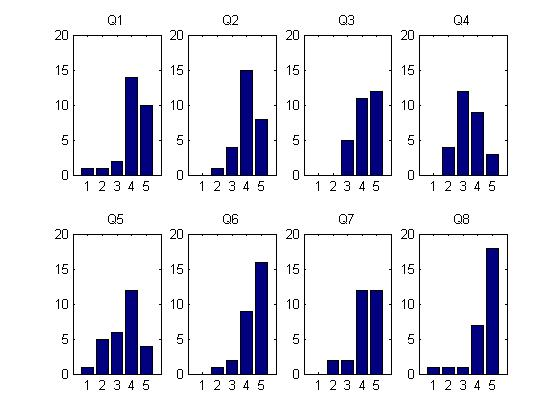
\includegraphics[width=5.5in]{histogram.jpg}
\caption{Histogram of Responses grouped by Questions}
\label{Fig:Figure6}
\end{figure}

Some of the observations from the important histograms include,
\begin{itemize}
\item Respondents are highly concerned about how their body mannerisms are perceived by their sighted peers (based on the response to Question 8 on the survey).
\item Facial expressions form the most important visual non-verbal cue that individuals who are blind or visually impaired feel they do not have access to (based on Question 6 on the survey). This correlates with the studies into non-verbal communication that highlights the importance of facial mannerisms and gestures, which are mostly visual in their decoding.
\item Followed by facial expressions, body mannerisms seem to be of higher importance for individuals who are blind and visually impaired (based on Question 3 of the survey).
\item The responses to questions 7, 1 and 2 suggest that respondents would like to know the identities of the people with whom they are communicating, relative location of these people and whether their attentions are focused on the respondent. This corresponds to knowing the position of their interaction partners when they are involved in a bilateral or group communication. People tend to move around, especially when they are standing, causing people who are blind to lose their bearing on where people were standing. This can result in individuals addressing an empty space assuming that someone was standing there based on their memory.
\item The responses to questions 4 and 5 indicate that there was a wide variation in respondents' interest in (4) knowing the physical appearance of people with whom they are communicating and (5) knowing about changes in the physical appearance of people with whom they are communicating. Many respondents indicated moderate, little, or no interest in either of these areas.
\end{itemize}

\subsection{Response Ratio}
Figure \ref{Fig:Figure7} shows the number of times the respondents chose to answer the 8 questions with their agreement or disagreement. The y-axis has been normalized to 100 points. The graph shows that respondents chose to answer the most by agreeing (Likert Scale 4) with the 8 questions. Followed closely behind was the strong agreement (Likert Scale 5) with the questions asked in the survey. The respondents chose to answer the least through strong disagreement (Likert Scale 1) to what was asked in the survey.

\begin{figure}
\begin{center}
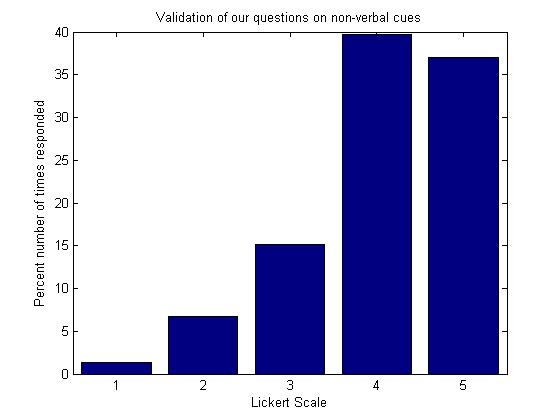
\includegraphics[width=5in]{responseratio.jpg}
\caption{Response Ratio}
\label{Fig:Figure7}
\end{center}
\end{figure}

As described earlier, the 8 questions corresponding to the social needs of the individuals were identified from the focus group survey that was conducted. Thus, the questions presented in the online survey questions were biased towards the needs of everyday social interactions of individuals who are blind and visually impaired. Thus, the implicit assumption while preparing this survey itself is that most of these items have been identified as being important and that only a priority scale needs to be extracted. This implicit assumption is immediately brought out by looking at the frequency with which the respondents answer with their agreement (Likert Scale 4) and strong agreement (Likert Scale 5).

\subsection{Rank Average Importance Map for Various Non-verbal Cues}
As can be seen from Figure \ref{Fig:Figure7}, the questionnaires were biased and the frequency of the responses is not Gaussian. This bias implies that using sample mean of the Lickert Scale responses will immediately show the same bias. This is due to the Gaussian iid assumption that is made while extracting the mean for the answers. In order to overcome this non-Gaussianity, we resort to non-parametric mean for the responses. Rank average of the responses is estimated instead of the typical mean of the responses for each of the question. Please see Appendix \ref{AppendixA} for the algorithm to determine the Rank Average. Since no assumptions on the distribution of the response are made, unlike the mean, the rank average gives a non-parametric method for comparing the responses of the individuals. The ranks can be either assigned ascending or descending with respect to the responses, i.e. rank 1 could mean all responses that were answered with strongly disagree (numeral 1), or rank 1 could mean all responses that were answered with strongly agree (numeral 5).

\begin{figure}
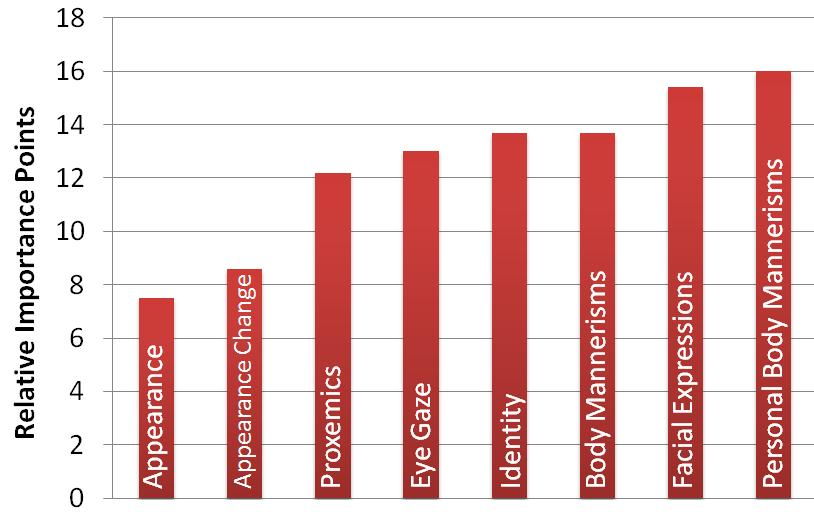
\includegraphics[width=5in]{rankaverage.jpg}
\caption{Rank average of the 8 questions}
\label{Fig:Figure8}
\end{figure}


In the Figure \ref{Fig:Figure8}, we have assigned rank 1 to strongly disagree. This is for the sake of visual convenience. Thus, higher the average rank, higher is that group's response from the respondents. Comparing Figure \ref{Fig:Figure8} to Table \ref{Tab:Table5}, it can be seen that the same ordering of priority can be seen through mean and rank average. But the mean tends to show very little variation between responses due to the bias that is present in the questions. On the other hand the rank average provides a good comparison scale.

\chapter{DETECTING STEREOTYPIC BODY MANNERISMS}
STEREOTYPIC behavior refers to any mannerism or utterance that is repetitive and non functional in nature \cite{thompson_stereotyped_1995} \cite{jankovic_stereotypies_1994}. Stereotypy occurs in a large portion of the general population in various forms, although aggressive forms have been associated with sensory and cognitive disabilities in individuals. For example, individuals who are blind have the tendency to develop body rocking, head weaving, head drooping, and eye poking \cite{mcadam_self-monitoring_1993}, while, individuals who are deaf have a propensity to develop various repetitive vocal behaviors \cite{reivich_behavior_1972}\cite{haag_repetitive_1985}. Cognitive disabilities (both acquired, like brain injury and congenital, like autism and mental retardation) are associated with stereotypic behaviors like body rocking, hand flapping, jumping, and marching in place \cite{shabani_reducing_2001}.

Though harmless by itself, Stereotypy can become a hindrance to social interactions and social acceptance \cite{loftin_social_2008}. Reference \cite{felps_modification_1988} introduces a 21 year old congenitally blind student who has an extreme case of body rocking (both while sitting and standing) that has become an obstruction to his career and an independent vocational evaluation states that a reduction in the student's body rocking was absolutely necessary for any form of employment. Stereotypy is a concerning problem in children, for whom peer acceptance is very important for their healthy growth and development of good social skills \cite{yu_loneliness_2005}. Children with stereotypic behaviors become victims of teasing thereby leading to social isolation, bullying and social segregation leading to negative self esteem. Aggravating these problems, social segregation and isolation have long term psychologically effects on the individual rendering an overall poor social skill set. Studies have shown that poor social skills are a leading cause for psychological problems such as depression, loneliness, and social anxiety \cite{segrin_poor_2000}.

Stereotypy, like any other human behavior, is very person specific. But socio-behavioral studies have shown that there are commonalities in these behaviors and there are broad classifications that can be identified in stereotypy prevalent in the general population. Eichel \cite{eichel_taxonomy_1979} introduces taxonomy for mannerisms that people with blindness and visual impairment tend to display. He identifies that body rocking appears on top of the most commonly seen behavior stereotype. A review of literature \cite{blasch_blindisms:_1972} further supports the claim that body rocking and head related mannerisms, including head weaving and drooping, are distinctive behaviors exhibited by individuals who have sensory or cognitive disabilities.  For example, \cite{mcadam_self-monitoring_1993} discusses the case of a blind student who has developed extreme body rocking stereotype. The student bends in a 30 degree arc when he is sitting and when standing, places a foot well ahead of him and bends forward in an even greater arc. Such stereotypes can hinder the interactions of these individuals with friends and family, eventually leading to isolation and social inadequacy in their personal and professional life.

\section{Focus of the chapter}\label{ResearchQuest}
Having identified stereotypic body behaviors to be an important deterrent in social acceptance of individuals with cognitive or physical disabilities, we focus on the possibility of building a rehabilitative and/or assistive technology towards providing feedback to individuals about their stereotypic body behavior. Specifically, we focus on body rocking, as it tops the list of most widely seen stereotypic behaviors. To this end, our research aims to answer three important questions:

\begin{enumerate}[1.]
\item Is there any evidence of individuals responding to rehabilitation for reducing stereotypic body rocking behavior?
\item If yes, what is the state-of-the-art technology available to detect and notify individuals of their rocking behavior?
\item Is it possible to build a device that detects body rocking condition and how well can it distinguish body rocking from other functional activities of daily living?
\end{enumerate}

We answer the first question by looking into the immense literature available in behavioral psychology which has been studying behaviors in humans and their response to rehabilitation and assistance. To answer the second and third questions, we focus our attention towards wearable computing solutions that have gained a lot of momentum in the recent past. In specific, we develop an argument for an inclusive framework that uses state-of-the art motion sensors with effective learning algorithms for detecting stereotype body rocking. As mentioned above, body rocking seems to be the most widely seen stereotype behavior and we use it as a basis for our argument that current level of technology can provide immense opportunities for developing rehabilitative and assistive technology solutions for reducing or controlling stereotypic behaviors.

\section{Background and Related Work}\label{BackGandRelatedWork}
\subsection{Foundations for social rehabilitation of behavioral stereotypes}
For over three decades, researchers in behavioral psychology have been publishing case studies on individuals who exhibit stereotypic body rocking. Most of these studies have targeted at reducing or controlling stereotypic body rocking. The methodologies used by these researchers, though varying in nature, can be broadly classified into two important categories.

\subsubsection{\emph{Intervention}}: Intervention relates to any form of feedback provided to an individual at the moment of exhibiting stereotype behaviors. Researchers have attempted to reduce body rocking by providing audio and/or tactual intervention whenever an individual started to rock. They have tried aversive punishment as well as less restrictive positive feedback in such situations. Felps and Devlin \cite{felps_modification_1988} issued an annoying tone in the ears of the subject while \cite{blasch_blindisms:_1972} used a recording of stone scratching on blackboard as the feedback tone whenever the individual started rocking. Both reported that the subjects responded well to the intervention. In contrast, \cite{raver_modification_1984}, \cite{raver_modification_1984} and \cite{ohlsen_control_1978} have used verbal praise, physical guidance, verbal reprimands, and brief time-outs as intervention tools. Most of these researches have shown that intervention has worked in reducing and controlling body rocking without the use of aversive techniques. Aversive or not, these techniques validate a claim that it is possible to control or reduce body rocking (or any other stereotypic body mannerism) through feedback.

\subsubsection{\emph{Self Monitoring}}: In contrast to intervention, self-monitoring does not stop at intervening into the activities of the individual. It attempts to teach these individuals subtle cognitive skills to replace the current mannerism with more socially acceptable behavior, exercise, or medications. McAdam and O`Cleirigh \cite{mcadam_self-monitoring_1993} identifies that self monitoring is a very effective way of reducing the body rock behavior. They introduce the case of a congenitally blind individual who is trained (with constant monitoring and positive feedback) to count the number of body rocks he goes through. Researchers noticed that the individual slowly waned off body rocking as he came to recognize and count his body's oscillatory movements. The research concludes that a well designed self monitoring program could benefit in reducing stereotypic body rocking. Shabani, Wilder and Flood \cite{shabani_reducing_2001} presents the case of a 12 year old child who was diagnosed with attention deficit hyperactivity disorder (ADHD) having an excessive body rocking and hand flapping stereotypy. The authors introduce an elaborate and positively rewarding self monitoring scheme that allows the child to improve on his behavior effectively. A follow-up with the child's teacher indicated that the social outlook of the child had improved over the course of rehabilitation and the case further reiterates ability to rehabilitate individuals with stereotypic behavior. Estevis and Koenig \cite{estevis_cognitive_1994} introduces a cognitive approach to reducing body rocking on an 8 year old congenitally blind child through self monitoring. Teachers or family members would tap on the shoulders of the child when he started rocking, while the child was taught to recite his own monitoring script. The authors conclude that rocking can be significantly reduced through notification to the individual combined with self monitoring.

Supporting such case studies of behavioral mannerisms, psychologists have been studying intervention and feedback as an integral component of social development. Feedback can be defined as the provision of evaluative information to an individual with the aim of either maintaining present behavior or improving future behavior \cite{schloss_increasing_1994}. According to \cite{cartledge_teaching_1986}, feedback is critical to social development because after an individual receives information about his or her performance, he or she can make the necessary modifications to improve social skills. Most social skills develop during early years and in order for children to evaluate themselves accurately and to modify social skills, it is essential that children to be given feedback \cite{jindal-snape_generalization_2004} \cite{jindal-snape_using_1998}, since without clear feedback, the children are unable to identify how their social behavior differs from others or is perceived by others in the environment \cite{raver_increasing_1988}. Based on these studies there is enough evidence that feedback that offers intervention, possibly followed by a well planned self-monitoring program could benefit in reducing or controlling body rocking behavior.

\subsection{Need for Assistive or Rehabilitative Technology}
The feedback needed for intervention usually comes from people in and around these individuals who have stereotypic behavior. It has been observed that significant others in the environment often fail to give feedback, and even when they do, it is not meaningful or understandable to individuals who need rehabilitation - for example, in case of individuals who are blind or visually impaired, nodding one's head in reply to a question or gesturing \cite{jindal-snape_use_2005} would be futile. Meaningful feedback is important, not only for social interaction, but for accurate self-evaluation by individuals. Most times people within the vicinity of individuals with needs fail to offer these crucial feedbacks. Many times, the individuals with needs feel guilty or obligated to ask for help from others in their environment. The ability to augment or replace this significant individual(s) in the environment with a reliable feedback mechanism is the aim and goal of all assistive technology solutions (In an independent online survey conducted by \cite{krishna_systematic_2008}, the researchers found that people who are visually impaired would expressed the need for an assistive technology that would provide feedback on their own social mannerisms and offer a potential to improve their social outlook). Focusing on the development of such a technology that effectively detects body rocking and provides feedback to an individual is the goal of this paper. While we focus only on intervention through feedback, in the Future works section we highlight some ideas for extending the proposed framework into self-monitoring tools.

\subsubsection{Past research into building assistive technology to detect body rocking}\label{BandRWC}
Transon \cite{transon_using_1988} developed a head mounted switching device that would trigger a tone when an individual starts to rock. The device consisted of a metal box with a mercury level switch that detects any bending actions. The feedback was provided with a tone generator that was also located inside the metal box.  The entire box was mounted on a strap that the user wears around his/her head such that the speaker aligns with the ears. The authors tested it on a congenitally blind individual who had severe case of body rocking and they conclude that the use of any assistive technology is useful only temporarily while the device is in use. They state that the body rocking behavior returned to baseline levels as soon as the device was removed. Since the time of this experiment, behavioral psychology studies have explored short term feedback for rehabilitation \cite{jindal-snape_use_2005} and these studies support the above observation that short time feedback is most of the times detrimental to rehabilitation and subject's case invariably worsens. Unfortunately, due to the prohibitively large design of the device developed by these researchers, it was impossible to have the individual wear the device over long durations. Thus, any technology developed for behavioral rehabilitation should be small and researchers should target the use over long durations in such a way that the feedback is slowly tapered off over a significantly longer duration of time.

Similar to the pervious experiment, \cite{felps_modification_1988} used a 'Drive Alert' (driver alerting system that monitors head droop) to detect body rocking and provide feedback to a congenitally blind 21 year old student. The research concludes that they were able to control body rocking effectively, but the device could not differentiate between body rocks from any other functional body movements. This device, primarily built to sense drooping in drivers provides no opportunity to differentiate between a body rock and a droop. Use of such devices could only be negative on the user as a large number of false alarms would only discourage an individual from using any assistive technology.
Assessing these above technologies, we resort to two important design dimensions in every step of the building of our assistive device.

\begin{enumerate}[1.]
\item Size and placement of the device: We argue that any assistive device developed for the sake of improving social outlook of an individual should respect the appearance of a person in his/her social circle and should provide a solution that is discrete and non intrusive. We call this the Acceptance dimension.
\item Ability to discriminate rocking from other functional activities:  False feedback even over a short period of time could be discouraging for an individual to continue using his/her assistive tool. It is imperative that the device be able to distinguish between the stereotypy from any other form functional activities effectively to keep the motivation of device use high. We call this the Motivation dimension.
\end{enumerate}

The proposed methodology uses these two design dimensions while addressing the need of a new assistive technology.

\section{Methodology}
Recently, human activity detection and recognition using motion sensors have taken a front seat in technology and behavioral research. This is due to the availability of micro mechanized electronic systems (MEMS) that have started to implement complex mechanical systems at a micro scale on integrated circuit chips. These offers advantages like reliability, cheaper cost of production, smaller form factor and above all extremely precise measurement with least or no maintenance. One such sensor is the accelerometer that is capable of measuring the effect of gravity on three perpendicular axes. When mounted on any moving object, the opposing motion (opposing gravity) of the entity allows these sensors to measure the speed and direction of motion. Integrating the magnitude and orientation information over time it is possible to accurately measure the exact motion pattern of the moving entity. These accelerometers have been used by researchers to track motion activity in almost every joint of the human body \cite{bao_activity_2004}. Researchers have used single, double or triple orthogonal axis accelerometers to detect various activities of humans. They all follow the same underlying supervised learning architecture with difference in learning algorithm used. A simplified representation of the same is shown in Figure \ref{JMMFigure1}.

\begin{figure}
\centering
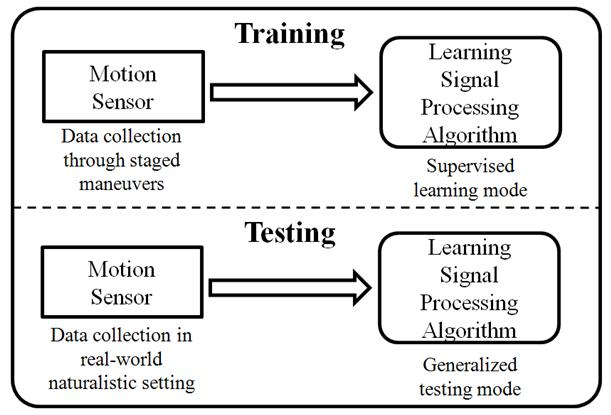
\includegraphics[width=4in]{JMMFigure1.JPG}
\caption{Training and testing phases of a typical learning framework found in literature.}
\label{JMMFigure1}
\end{figure}

 Five bi-axial accelerometers are used in \cite{bao_activity_2004}, along with a decision tree classifier to detect and recognize 20 different activities of daily life. They report a recognition rate of over 85\%. In \cite{ravi_activity_2005}, the authors evaluated different meta classifiers for recognizing seven lower body motion patterns from a single biaxial accelerometer data and reported the best performance for boosted Support Vector Machines (SVM) \cite{cristianini_introduction_2000} with a subject independent accuracy of 64\%. Since each dimension of the accelerometer data is similar to audio waveform, popular Hidden Markov Models \cite{rabiner_tutorial_1989} can be used to learn motion patterns. Reference \cite{amft_detection_2005} used HMM to learn the accelerometer data for specific tasks performed by participants and reports a recognition rate of over 90\%. In \cite{chambers_hierarchical_2002}, researchers have used two accelerometers placed on the arms of Kung-Fu practitioner and report a recognition accuracy of 3 Kung-Fu arm movements at 96.6\%. Research work \cite{seon-woo_lee_activity_2002} demonstrates the use of accelerometer data to not only recognize activity, but also localize people within a building. Though the technique is rudimentary, the authors report a high accuracy in recognition of activities while localization still remains a research topic. \cite{foerster_detection_1999} have demonstrated the use of accelerometers in not only monitoring movements, but also static posture of the human body. They report a recognition rate of 95\% using four sensors placed on the chest, thigh, forearm and wrist of participants. Extending this work, \cite{arteaga_low-cost_2008} have demonstrated an assistive technology solution that uses low cost accelerometers on stroke patients and monitor their posture and walking patterns. Using this information, a feedback is provided to the patient to self-correct their posture and walking pattern.

Based on all these findings, we hypothesize that an accelerometer based motion detector should be capable of capturing body rocking data and should be able to discriminate between rocking and other functional activities. We specifically chose the motion sensor and learning algorithm based on previous work done at our institute with the detection of seven simple body activities \cite{krishnan_analysis_2008}. Researchers analyzed the performance of discriminative classifiers like AdaBoost, Support Vector Machines and RLogReg for recognizing these seven different activities and concluded that AdaBoost classifier offered the best recognition rate at 94\%. Based on these results, in this paper, we extend the use of AdaBoost learning framework into body rock detection. We discuss the use of two AdaBoost classifiers - the classical AdaBoost \cite{polikar_ensemble_2006} and the more recent Modest AdaBoost \cite{vezhnevets_modest_2005} for detecting and discriminating body rocking effectively. Our focus in the paper is directed towards understanding the generalization capabilities of the two AdaBoost learning models so that false positive rate is reduced while keeping the true positive rate high.

\subsection{Motion Sensors - Design choice along the ``Acceptance'' Dimension}
In order to keep the motion detector discrete, we have chosen state-of-the-art tri-axial accelerometer package, ZStar III \cite{_drm103_2008}, marketed by Freescale Semiconductor. The accelerometer is shown in the inset of Figure \ref{JMMFigure2}. The device (including a coin battery as a power source) is an inch in diameter and less than eighth of an inch in thickness thereby allowing an elegant integration into everyday clothing. Figure \ref{JMMFigure2} shows the typical use of the accelerometer in the proposed application for detecting body rocking. The accelerometer has a very high sensitivity with protection against excessive g-force damage. The sensors wirelessly connect to a PDA and/or cell phone through IEEE 802.15.4 (ZigBee) wireless standards. The use of low power consumption electronics for both acceleration sensing and wireless communication allows this device to work for hours at length on a single coin battery. Further, the advanced sleep mode implementations allow the device to stay at nano watt power mode during non-operation. The proposed solution allows for prolonged use of the device to the effect of an assistive technology thereby maintaining a longer duration feedback based rehabilitation regimen.

\begin{figure}
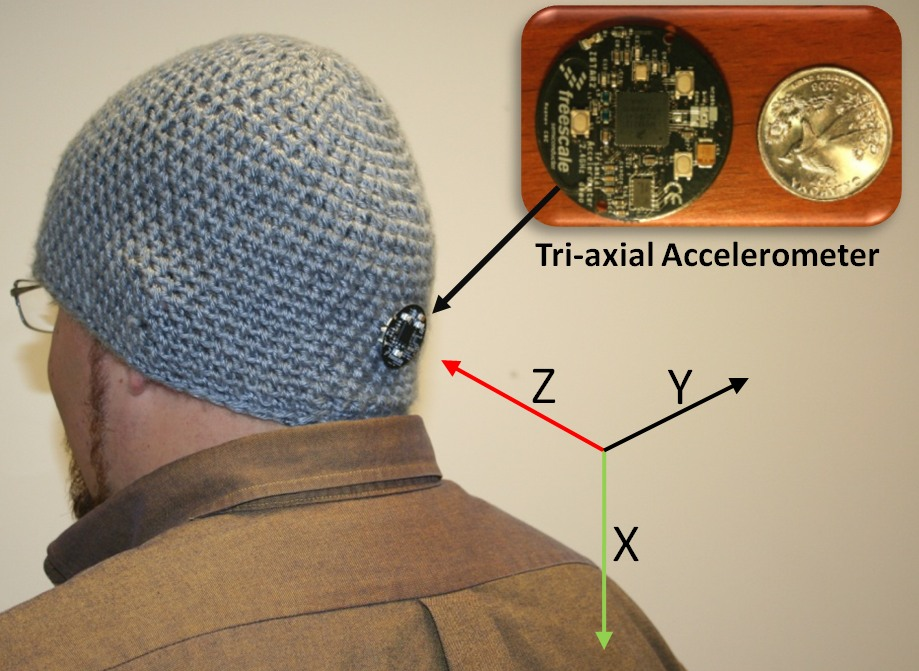
\includegraphics[width=4.5in]{JMMFigure2.JPG}
\centering
\caption{The proposed hardware for use in the detection of body rocking stereotypic behavior. The accelerometer, in comparison with a US quarter, is shown in the inset. The three axes marked in the image shows the orientation of the accelerometer as it is placed on the head.}
\label{JMMFigure2}
\end{figure}

processing element for the current study was a Windows Mobile Operating System based PDA running on a 400Mhz XScale processor. The software components (described in detail in Section III-B of the proposed solution were placed on the PDA that could be carried by a user without any extra load. The proposed assistive technology is a planned addition on top of the Social Interaction Assistant proposed in \cite{krishna_wearable_2005}.  The software component implementation is generic to be ported to most modern cell phones that possess enough processing power, but is always underutilized for its capacity. The feedback (an audio tone) is currently being provided through a Bluetooth headset that is paired with the processing element. The choice of this feedback device was again based on the idea that Bluetooth headset has everyday acceptance among the masses and is no longer seen as a social distraction. In future, we plan to explore the use of delivery modalities that transcends the typical visual and audio medium. We intend to use haptic cues to inform the participant not only their rocking behavior but more complex self-monitoring routines that could allow the user to withdraw from the rocking behavior effectively.

\begin{figure}
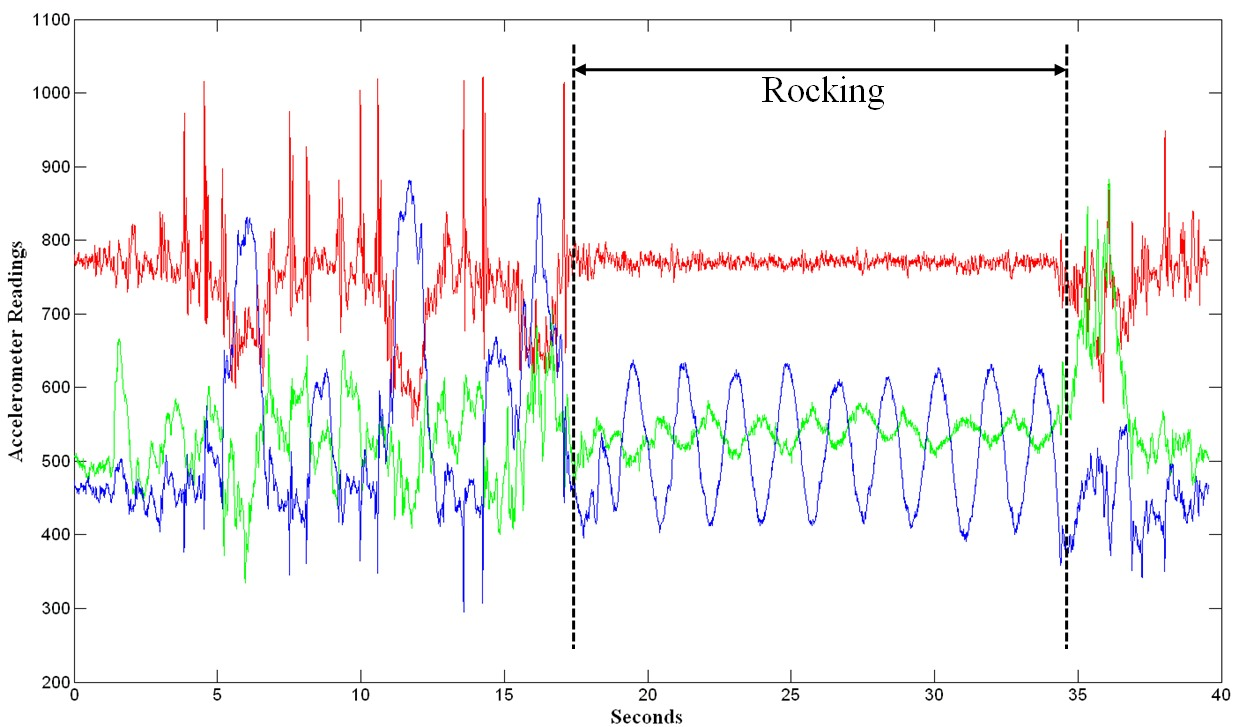
\includegraphics[width=5.5in]{AccelerometerData.jpg}
\caption{Data stream for the tri-axial accelerometer. The three streams correspond to the three axes. The figure shows non-rocking events followed by rocking and then followed by non-rocking.}
\label{JMMFigure3}
\end{figure}

Figure \ref{JMMFigure3} shows a typical data stream collected from the accelerometer shown in Figure 2 during rocking and non-rocking functional behavior. The three data streams correspond to the three axis of the accelerometer each sampled at 100 Hz. It can be seen that the data stream under rocking conditions are visually distinguishable when compared to non-rocking functional movements. The following section highlights our choice of learning framework and features we extracted from these data stream in order to achieve reliable rocking and non-rocking discrimination.

\subsection{Extracting Body Rock Information from Motion Sensor Data - Design choice along the ``Motivation'' Dimension}
As mentioned before, the work presented in this paper builds on top of the work presented in \cite{krishnan_analysis_2008} where the authors use two accelerometers placed one at the ankle and the other on the thigh to distinguish between simple activities like walking, running, standing etc. They proved the use of an aggregated AdaBoost classifier system that was built out of simple linear classifiers to achieve activity recognition. Unfortunately, the work does not provide any assessment on the generalization capabilities of their aggregate classifier. We extend their work into the problem of body rock detection using only one accelerometer placed on the back of the person's head. Below, we discuss the various features that we extract from the accelerometer data and introduce the variant of AdaBoost that generalizes on its training set very well (termed Modest AdaBoost). We show results of our experiments and discuss our reasoning to believe how the new AdaBoost framework is able to generalize on body rocking data when compared to classical AdaBoost used by [36].

\subsubsection{Features:}
Since we are using a tri-axial accelerometer, we obtain three orthogonal axis data through rocking and non-rocking events. In order to capture the temporal variation in the acceleration data, we accumulate the input stream on each axis for a fixed duration T seconds and all features are extracted on this packet of acceleration data. As a part of the assessment, we determine the best packet length for the task of body rock detection. Further, successive packets are extracted with a fixed duration of overlap between them.

We chose five sets of features that were extracted on the three axes of accelerometer data. For the sake of clarity, we cluster these sets into two groups based on whether they were chosen due to popular use in the accelerometer data processing community or due to the author's insights into the body rocking data.

\emph{Group 1 - Popular features used by the motion analysis research community \cite{bao_activity_2004} \cite{krishnan_analysis_2008}:}
We choose the following three sets each of which were applied on all three axes of acceleration data, henceforth referred to as x, y, z axis data.

\begin{enumerate}[1.]
\item Mean of x, y, z data over the duration of packet.
\item Variance of x, y, z data over the duration of packet.
\item Correlation between the three axes (x-y, y-z and z-x) over the duration of packet.
\end{enumerate}

\emph{Group 2 - Authors insights into body rocking data:} Inspecting the accelerometer data shown in Figure 3, it can be seen that the Z axis changes from random signal pattern to more of a sinusoidal pattern when the individual's behavior transitions from non-rocking to rocking. Thus we choose two sets of features which we hope would capture this non-sinusoid to sinusoid transition between events. These features include

\begin{enumerate}[1.]
\setcounter{enumi}{3}
\item The first order differential power on all three axes - Sinusoidal signals change gradually over time such that the averaged sum square energy in the temporal first order differential of the signal should be less when compared to a random signal where the first order differential can have very high variations and hence higher power.
\item Fourier Transform variance and kurtosis on the Z-axis only - An effective way to capture power distribution of a signal into sinusoids is by using Fourier Transform. We hypothesize that the non-sinusoid to sinusoid transitions can be captured by quantitatively measuring the power spread spectrum of the Z-axis accelerometer data. We model the power spread to be a Gaussian and extract the variance and kurtosis (peaking) of the spread to determine if there is rocking or not.
\end{enumerate}


\begin{landscape}
\begin{table}
\centering
\caption{Features for Body Rock Detection: Group 1}
\label{JMMTable1}
\small\addtolength{\tabcolsep}{-3pt}
\begin{tabular}{|l|c|c|c|} \hline
\multicolumn{4}{|c|}{\textbf{Group 1}}\\
\hline
\hline
  \textbf{Set 1} & \multirow{9}{*}{$M_x=\frac{1}{N}\sum\limits_{i=1}^{N}x_i$} & \multirow{3}{*}{1. $M_x$} & \multirow{9}{*}{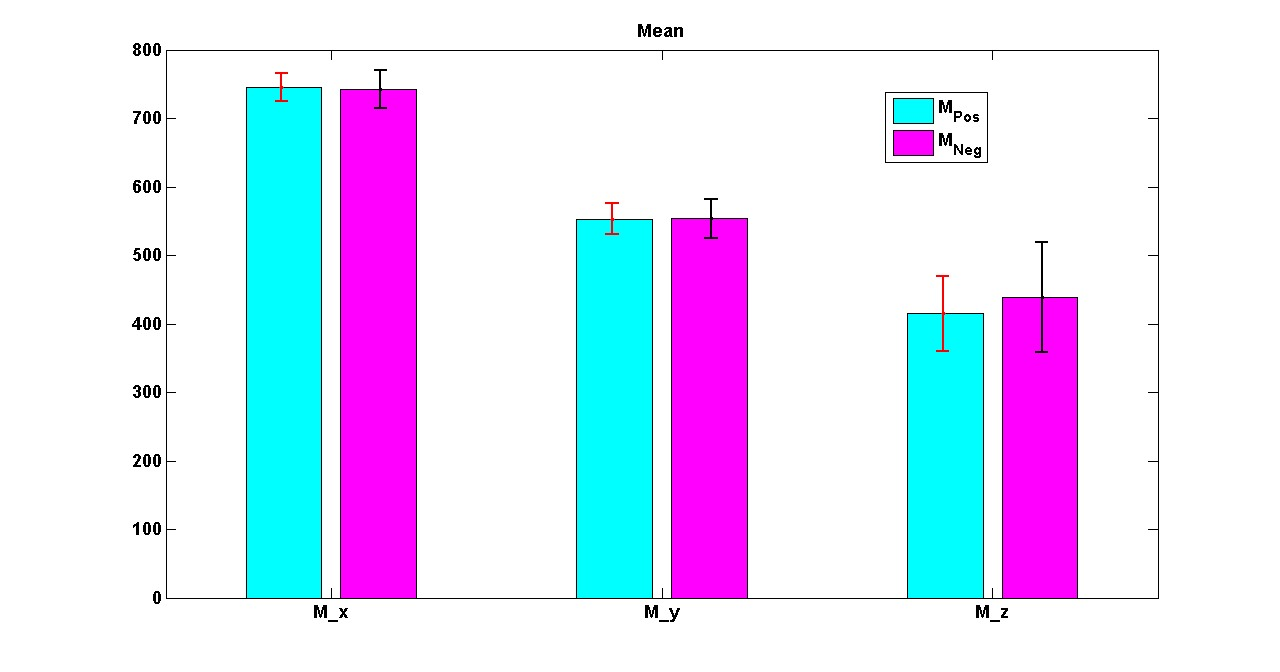
\includegraphics[width=3in]{Mean.jpg}}\\
                 &                                                            &                        &       \\
                 &                                                            &                        &       \\
  \textbf{Definition:} Mean on the temporal dimension. &                      & \multirow{3}{*}{2. $M_y$} &       \\
  \textbf{Axes affected:} x, y, z                      &                      &                        &       \\
  \textbf{Number of contributing features:} 3          &                      &  &       \\
  \textbf{Feature Identification Numbers:} 1, 2, 3     &                      & \multirow{3}{*}{3. $M_z$}                       &       \\
                 &                                                            &                        &       \\
                 &                                                            &                        &       \\
\hline
  \textbf{Set 2} & \multirow{9}{*}{$V_x=\frac{1}{N-1}\sum\limits_{i=1}^{N}\left(x_i - M_x\right)^2$} & \multirow{3}{*}{4. $V_x$} & \multirow{9}{*}{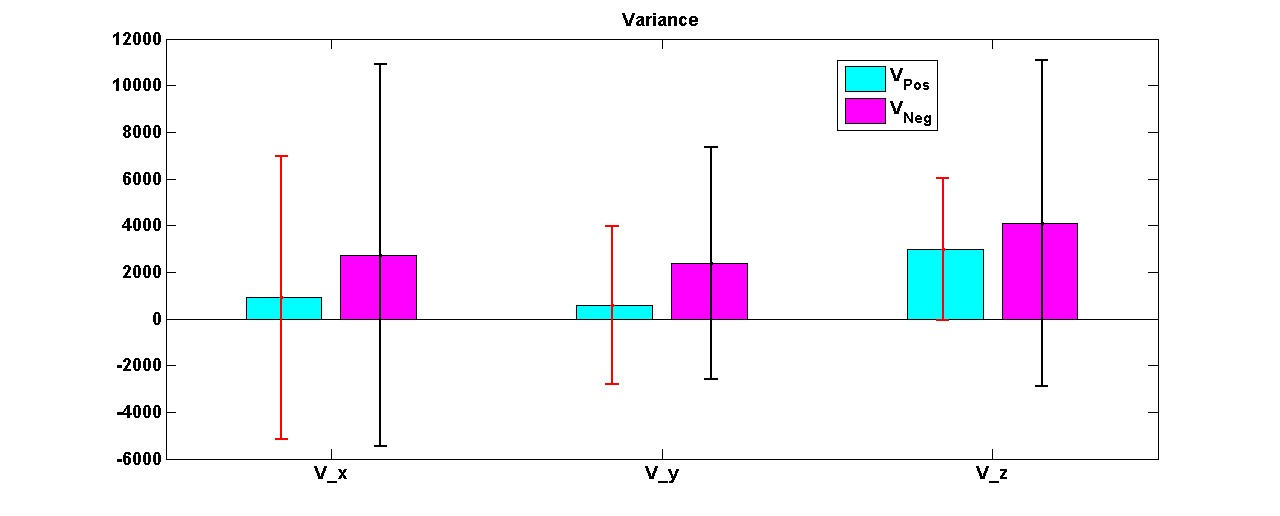
\includegraphics[width=3.5in]{Variance.jpg}}\\
                 &                                                            &                        &       \\
                                  &                                                            &                        &       \\
  \textbf{Definition:} Variance on the temporal dimension. &                  & \multirow{3}{*}{5. $V_y$} &       \\
  \textbf{Axes affected:} x, y, z                      &                      &                        &       \\
  \textbf{Number of contributing features:} 3          &                      &  &       \\
  \textbf{Feature Identification Numbers:} 4, 5, 6     &                      &  \multirow{3}{*}{6. $V_z$}                      &       \\
                   &                                                            &                        &       \\
                                    &                                                            &                        &       \\
\hline
  \textbf{Set 3} & \multirow{9}{*}{$C_{xy}=\frac{1}{N-1}\sum\limits_{i=1}^N \left(x_i-M_x\right) \left(y_i-M_y\right)$} & \multirow{3}{*}{7. $C_{xy}$} & \multirow{9}{*}{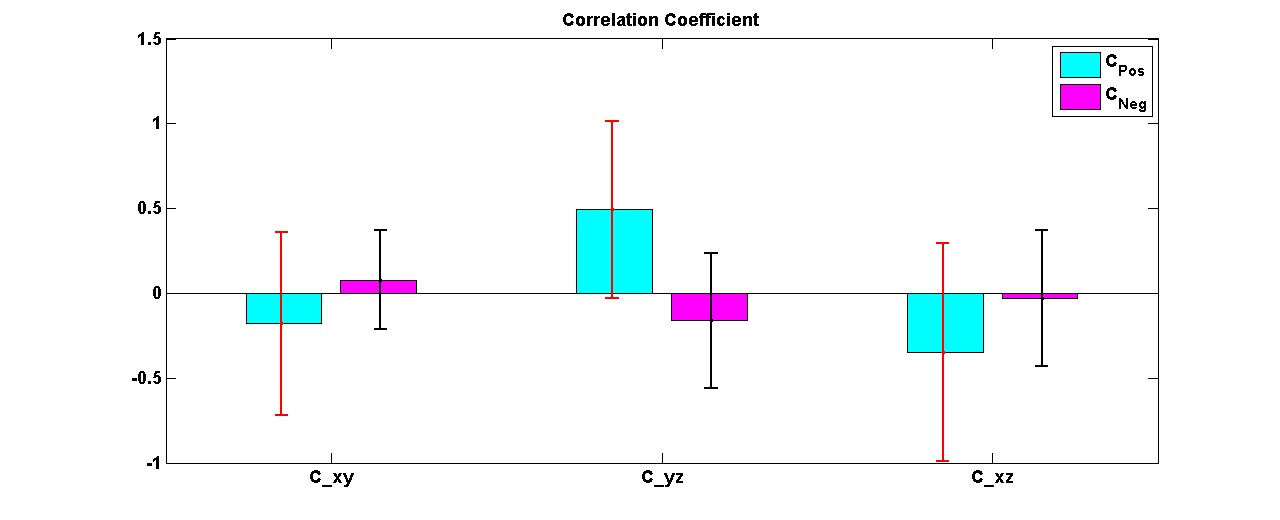
\includegraphics[width=3.5in]{Corr.jpg}}\\
                 &                                                            &                        &       \\
                                  &                                                            &                        &       \\
  \textbf{Definition:} Cross Correlation between axes. &                      & \multirow{3}{*}{8. $C_{yz}$} &       \\
  \textbf{Axes affected:} x, y, z                      &                      &                        &       \\
  \textbf{Number of contributing features:} 3          &                      &  &       \\
  \textbf{Feature Identification Numbers:} 7, 8, 9     &                      &   \multirow{3}{*}{9. $C_{xz}$}                     &       \\
                   &                                                            &                        &       \\
                                    &                                                            &                        &       \\
\hline
\end{tabular}
\end{table}
\end{landscape}

\begin{landscape}
\begin{table}
\centering
\caption{Features for Body Rock Detection: Group 2}
\label{JMMTable2}
\small\addtolength{\tabcolsep}{-3pt}
\begin{tabular}{|p{2.5in}|c|c|c|} \hline
\multicolumn{4}{|c|}{\textbf{Group 2}}\\
\hline
\hline
  \textbf{Set 4} & \multirow{9}{*}{$D_x=\sqrt{\sum\limits_{1=2}^N\left(x_i-x_{i-1}\right)^2}$} & \multirow{3}{*}{10. $D_x$} & \multirow{9}{*}{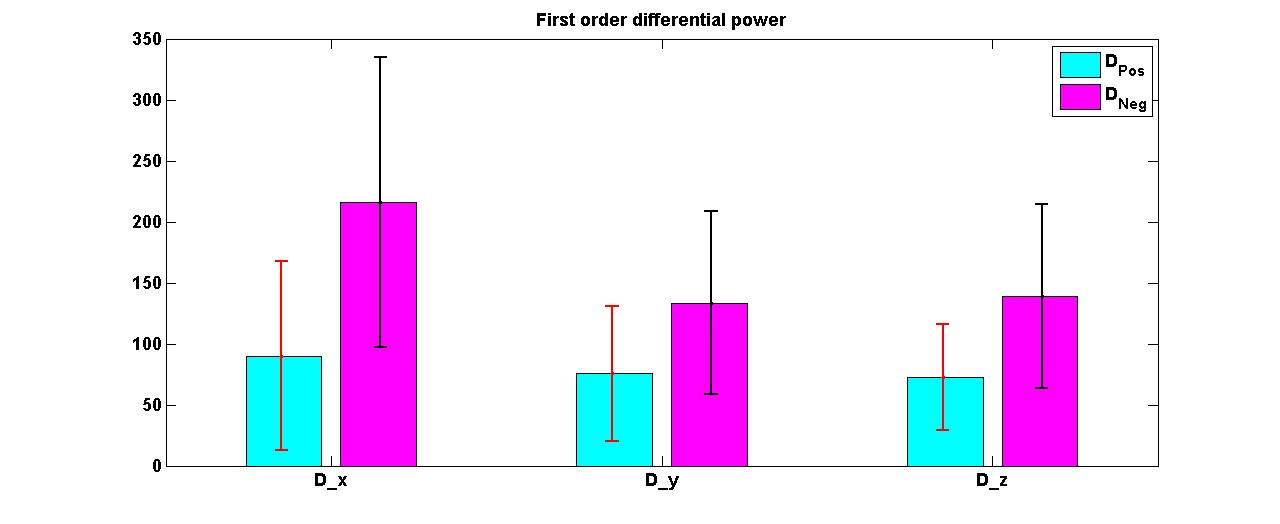
\includegraphics[width=3in]{DiffPower.jpg}}\\
                 &                                                            &                        &       \\
                 &                                                            &                        &       \\
  \textbf{Definition:} First order differential power. &                      & \multirow{3}{*}{11. $D_y$} &       \\
  \textbf{Axes affected:} x, y, z                      &                      &                        &       \\
  \textbf{Number of contributing features:} 3          &                      &  &       \\
  \textbf{Feature Identification Numbers:} 10, 11, 12     &                      & \multirow{3}{*}{12. $D_z$}                       &       \\
                 &                                                            &                        &       \\
                 &                                                            &                        &       \\
\hline
  \textbf{Set 5} & & \multirow{5}{*}{13. $F_{v_z}$} & \multirow{5}{*}{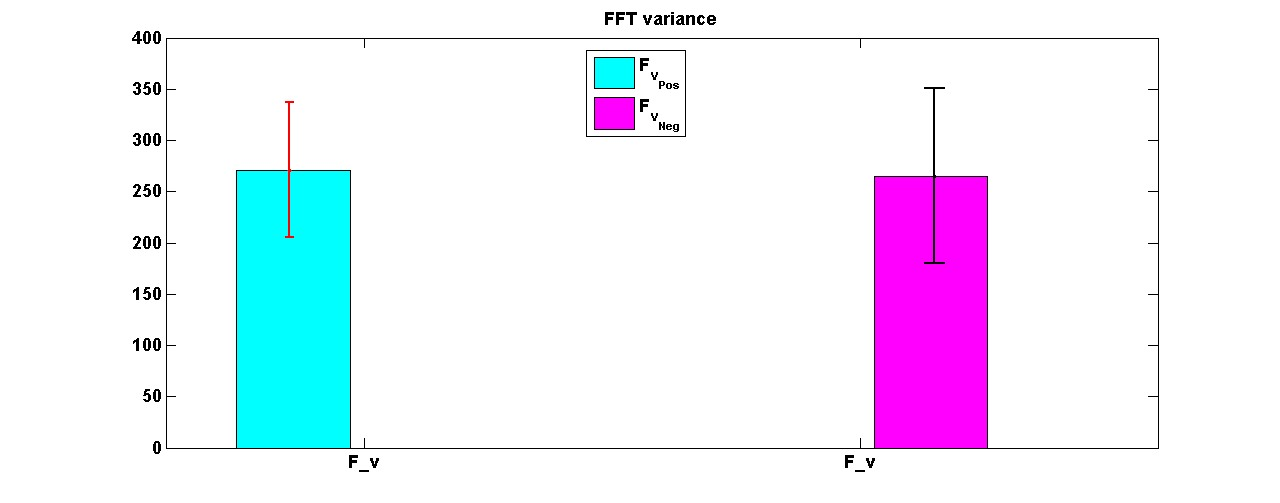
\includegraphics[width=3.5in]{FFTVar.jpg}}\\
  & If, $Freq_k=\left\{-\frac{\gamma}{2},\ldots,0,\ldots,\frac{\gamma}{2}\right\} $ &  &       \\
  &&&\\
  & $\gamma$ is the sampling Frequency & & \\
  \textbf{Definition:} Gaussian fit power spread spectrum - Variance and Kurtosis. & $X_k=\sum\limits_{i=1}^Nx_n e^{-\frac{2\pi i}{N}kn}$, $k=\{1,\ldots,N\}$ &  &       \\
  \textbf{Axes affected:}z  &    &  \multirow{5}{*}{14. $F_{k_z}$}& \multirow{5}{*}{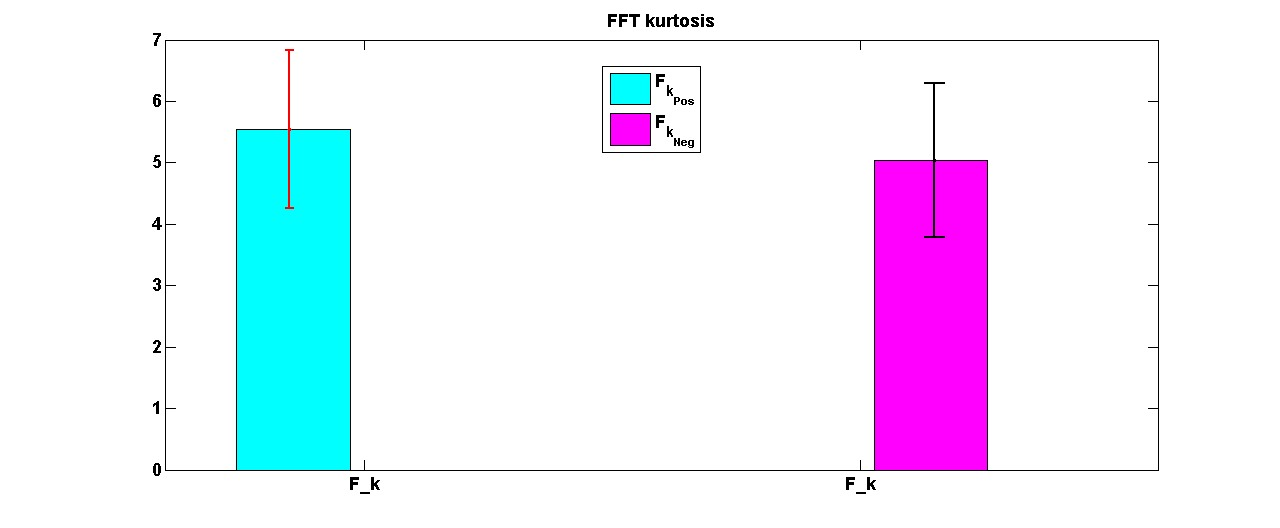
\includegraphics[width=3.5in]{FFTKurt.jpg}} \\
  \textbf{Number of contributing features:} 2          & then  &  &       \\
  \textbf{Feature Identification Numbers:} 13, 14     &                      &                        &       \\
  &   \textbf{FFT Variance:} $F_v = \sum\limits_{i=1}^N X_k(Freq_k)^2$  &                        &       \\
  &     &                        &       \\
  &  \textbf{FFT Kurtosis:} $F_k = \sum\limits_{i=1}^N X_k(Freq_k)^4$   &                        &       \\
  &     &                        &       \\
\hline
\end{tabular}
\end{table}
\begin{SingleSpace}
The figures shown in the last column plots mean values of data from positive rocking samples and negative rocking samples as bars. The variance on the same is shown as vertical error lines around the mean. The lighter (blue when viewed in color) shaded bar are values from the positive class, whereas the darker (pink when viewed in color) bar are values from the negative class.
\end{SingleSpace}
\end{landscape}

Thus, the features used in our study can be categorized as belonging to two groups with three sets in Group 1and two sets in Group 2. Each set has varying number of features based on what parameter the set is extracting from the temporal accelerometer data. Based on the descriptions above, the entire feature set has a total of 14 features. We identify each of these by their respective Feature Identification Numbers. Table 1 shows the two groups and the different sets under the group with typical values of these features under rocking and non-rocking behavior.

\subsubsection{Learning Algorithm:}
As discussed in introduction of this section, we compare the performance of two AdaBoost learning frameworks to determine which one can generalize the best on the training data. The two algorithms are introduced briefly below. For further details, the reader is referred to appropriate references provided within the subsections.

\emph{(a) Classical AdaBoost Learning Framework:}
AdaBoost learns any classification problem by working with a set of weak classifiers. Weak classifiers are those classifiers that use simple decision steps to categorize data into one of two pools - positives or negatives (In all our experiments, we used a three level decision tree \cite{yuan_induction_1995} as the simple classifier). AdaBoost proceeds by ranking the labeled training data as being simple to complex based on how many weak classifiers are needed to learn each of the examples. The process continues on an iterative manner until all the training examples are learnt or till the allowed number of learning cycles are exhausted. Let, $X$ be the input to a learning algorithm, in our case the features extracted as explained in the previous step, and $Y$ be the label of what class the data belongs to, in our case, $Y = \{1, -1\}$ implying {rocking, non-rocking}, respectively. Values at each dimension of input $X$ can be considered to characterize the incoming data in some manner and the task of the learning algorithm is to learn these representational values of the input dimensions that allow the algorithm to distinguish between rocking and non-rocking. AdaBoost does this learning by using a large set of simple (weak) learners (or classifiers) that act on each of the dimension of the input data with the determined goal of distinguishing rocking from non-rocking. The final decision of the complete learning module is a combined opinion of all the simple learners that make up the system. The beauty of AdaBoost implementation is that the human intervention into the learning process stops at identifying what simple (weak) learners to use and what feature pool to operate on. Selection of number of weak learners, selection of input dimension on which the weak learners have to act, and the confidence to place on the decision of each of the weak learner is all determined by the algorithm during the training phase. Once the algorithm is trained, the final learnt rocking/non-rocking classifier can be represented as

\begin{equation}
L(x)= \mbox{sign} \left[\sum\limits_{i=1}^N w_i f_i(x)\right]
\end{equation}

where,
x: An instance of all possible rocking patterns X.
L: The final learnt classifier that can distinguish input x as rocking or non-rocking.
f: The simple (weak) learner.
N: The total number of weak learners that make up the complete learner L.
w: Weight associated with each weak learners output. This corresponds to the confidence placed in each weak learner by the Boosted system.

From a learning perspective, in each step of the iterative learning, the AdaBoost algorithm implements a greedy optimization to pick a set of weak learners that minimize exponential classification error of the picked simple classifiers as shown below

\begin{equation}
Error_k=\sum\limits_{i=1}^M e^{-y_i.L(x_i)}
\end{equation}

where,
	y: Label of the input instance x
	M: Total number of examples in the training set
	k: Learning iteration number


Further, based on each iterative step, a distribution $(D_m)$ is created over the training set examples to represent their complexity (difficulty to learn). For example, in a given iteration, an example that could be solved is assigned a lower distribution weight while, a sample that was not learnt in that iteration step is assigned a higher weight. The lower weight on the learnt example implies that this example will be stressed less in the next learning iteration while all other examples which could not be solved will become the focus for picking new weak learners. Moving from one iteration to the next, all the weak learners from the past k iterations are added into a pool of selected weak learners leading up to the final classifier $L$.

\emph{(a) Modest AdaBoost Learning Framework:}
All learning algorithms, including AdaBoost suffer from the problem of over fitting or over learning. This is due to the fact that training sample sets of positives and negatives can never be representative of all the possible samples that the algorithm will face in its operational life span. Since the learning is limited to a restricted set of examples, there is always the problem of over fitting into this small set and thereby loosing the ability to generalize their learnt knowledge to all other possible examples. To this end, many alternatives have been proposed to AdaBoost that will allow the algorithm to generalize better. We introduce Modest AdaBoost \cite{vezhnevets_modest_2005} which was recently proposed towards better generalization capabilities and has been shown to be powerful on various machine learning datasets. Unlike the classic AdaBoost where the distribution penalizes only examples that are not learnt in the previous iteration, Modest AdaBoost penalizes for examples that are not learnt and also examples that are learnt very well (over fitting). This is done by projecting all the examples in the training pool on to four separate distributions,

\begin{enumerate}[1.]
\item $P_m^{(+1)}=P_{(D_m)} (y=+1 \cap L(x))$: Probability of the learner, as measured on $D_m$, predicting an input instance $x$ correctly as being rocking when the label also represents it to be rocking.
\item $P_m^{(-1)}=P_{(D_m)} (y=-1 \cap L(x))$: Probability of the learner, as measured on $D_m$, predicting an input instance $x$ correctly as being non-rocking when the label also represents it to be non-rocking.
\item $\bar{P}_m^{(+1)}=P_{(\bar{D}_m)} (y=+1 \cap L(x))$: Probability of the learner, as measured in the inverse distribution $(\bar{D}_m)$, predicting an input instance $x$ correctly as being rocking when the label also represents it to be rocking.
\item $\bar{P}_m^{(-1)}=P_{(\bar{D}_m)} (y=-1\cap L(x))$: Probability of the learner, measured in the inverse distribution $(\bar{D}_m)$, predicting an input instance $x$ correctly as being rocking when the label also represents it to be rocking.
\end{enumerate}

Conditions 1 and 2 penalize the classifier on examples that are not learnt during a training iteration, whereas 3 and 4 penalize examples that are already learnt in the previous iteration which was learnt again in the current iteration. Combining these four measures as

\begin{equation}
f_m=\left(P_m^{(+1)} (1-\bar{P}_m^{(+1)})-P_m^{(-1)} (1-\bar{P}_m^{(-1)})\right)(x)
\end{equation}

provides a means for penalizing the learner for not classifying an example and also for over fitting an example. This provides a means for modest learning of the final combined classifier $L$. We hypothesize that the choice of a learning algorithm that generalizes well will provide the opportunity to allow better non-rocking detection thereby hopefully increasing discrimination ability for the assistive device. This would directly reflect upon the motivation of the user to get feedback only when he/she is rocking and not performing other functional activities.

\section{Data Collection}\label{DataCollection}
Two separate data collections were carried out, one in a controlled setting while the other in a more uncontrolled naturalistic everyday research laboratory setting. The controlled setting data collection was used for training and lab testing the device, whereas the uncontrolled naturalistic setting was used to determine how well the learning algorithm was able to generalize when used for an extended period of time as an assistive tool.
\subsection{Controlled Data Collection:}
Data was collected on ten participants who did not have any known stereotype rocking behavior. The goal of the experiments was to collect data for training the system to differentiate rocking from non-rocking behavior. To this end, we devised three separate data collection routines where the subjects were required to do rocking and non-rocking tasks as naturally as possible. The details of the routines are as follows:

\subsubsection{	Routine A: Rocking data} \label{RoutineA}
Participants were allowed to choose from a rocking chair or a stool or sitting on the ground, so they could rock as comfortably and naturally as possible. We found some cultural preferences to the way people choose to rock. The subjects were asked to rock for a total of 20 complete cycles.

\subsubsection{Routine B: Non-rocking data}\label{RoutineB}
The participants were asked to do activities that did not involve rocking. They moved around the experimental setup reading posters, operating computers, interacting with everyday office equipments and included some functional body motions similar to rocking like, stooping down to pick up objects, rapidly bending down to pick up objects etc. Data was collected for a total of 30 seconds.

\subsubsection{Routine C: Test data}\label{RountineC}
Since rocking can happen at any given instance, we collected data where subjects did various activities and interspersed them randomly with rocking. The goal is to determine how fast and accurately our system can detect such rocking occurrences. In all of these data streams, rocking instances were manually identified and marked for the sake of ground truth. Figure 3 shows the combination of rocking and non-rocking activities by the participants. It can be noticed that there is a clear demarcation between the two activity zones.

\subsection{Uncontrolled Data Collection:}\label{Uncontrolled}
The uncontrolled data was collected towards testing the generalization capabilities of the learnt system. To this end, the body rock detection system was worn by the primary author during everyday laboratory activities. Body rock detection was provided as a feedback through a pair of headphones in the form of an audio beep. Five trails of four separate ten minute data collections were done. Two of the four were done with classic AdaBoost whereas the other two were done with Modest AdaBoost. Further, under each of these two classifiers, one data collection measured how many false positives were detected, whereas the second data collection counted how many rocking actions went undetected. During all these data collection the researcher counted the number of false positive or false negatives using a handheld thumb counter. This experiment was conducted purely to test the generalization capability of the learnt classifier.

\section{Experiments}
Experiments were carried out for comparing the performance of the classic AdaBoost framework with Modest AdaBoost for the specific tasks of determining
\begin{enumerate}[a.]
\item The length of a temporal packet of data needed to effectively distinguish rocking from non-rocking.
\item The accuracy with which the two classifiers can distinguish between rocking from non-rocking.
\item The generalization capabilities of the two classifier systems.
\end{enumerate}

To this end the rocking samples collected in Routine A (discussed under Section \ref{RoutineA}) and Routine B (discussed under \ref{RoutineB}) were used as labeled positive (rocking) and negative (non-rocking) data for training the AdaBoost classifiers. Data collected under Routine C (discussed in Section\ref{RoutineC}) were used for testing the learnt classifiers. The results from this analysis were used for determining a. and b. above. We varied the packet length on the data stream and determined the recognition rate on the test data. While the packet length was varied, a constant overlap was maintained between successive packets. This overlap was determined empirically to be 0.5 seconds or 50 samples (100 Hz sampling rate). With the ground truth already provided for the test set, we were able to determine the accuracy of the two classifiers.

To determine c., we resorted to using the data collected in Section \ref{Uncontrolled}. The primary author of the paper used the device to collect false positive and false negative data in order to determine how well the classifiers generalized on the training data. Further, we analyzed the working of the two classifiers in a piece wise manner by breaking down the features into individual sets (Sets 1 through 5 as identified in Table \ref{JMMTable1} and Table \ref{JMMTable2} and Set 6 that included all 14 features) and understanding the functional ability of the classifiers under individual feature sets. This allowed for an in-depth analysis of the workings of the two classifiers. In Section VII, we discuss the generalization capability of the two classifiers by heuristic analysis of the piecewise operational modes.

All our experiments were carried out with the aid of the AdaBoost Matlab library developed by Graphics and Media Lab at the Dept. of Computer Science at Moscow State University [42].

\section{Results}\label{ResultsJMM}
Figures \ref{JMMFigure4} and Figure \ref{JMMFigure5} shows the box plot \cite{benjamini_opening_1988} of packet length (T secs) versus recognition rate for classic AdaBoost and Modest AdaBoost frameworks, respectively. The abscissa represents the length of the data stream (in seconds) used for the analysis, while the ordinate represents the recognition rate. Training and testing were all carried out on the data collected as depicted in Section \ref{DataCollection}. The horizontal line inside the box represents the median (second quartile) of recognition rates over the ten subject's data. The lower end of box presents the first quartile (25 percentile) and the upper end of the box represents the third quartile (75 percentile). Thus the box surrounds the center 50 percentile ranges of recognition results. This box is also called the Inter-Quartile Range (IQR = third quartile - first quartile). The dotted extremity represents the minimum and maximum recognition rate under a certain packet length among the ten subjects. Any outlier (an outlier is greater than 1.5 IQR from the median in any direction) is marked by an asterisk.


\begin{figure}
\centering
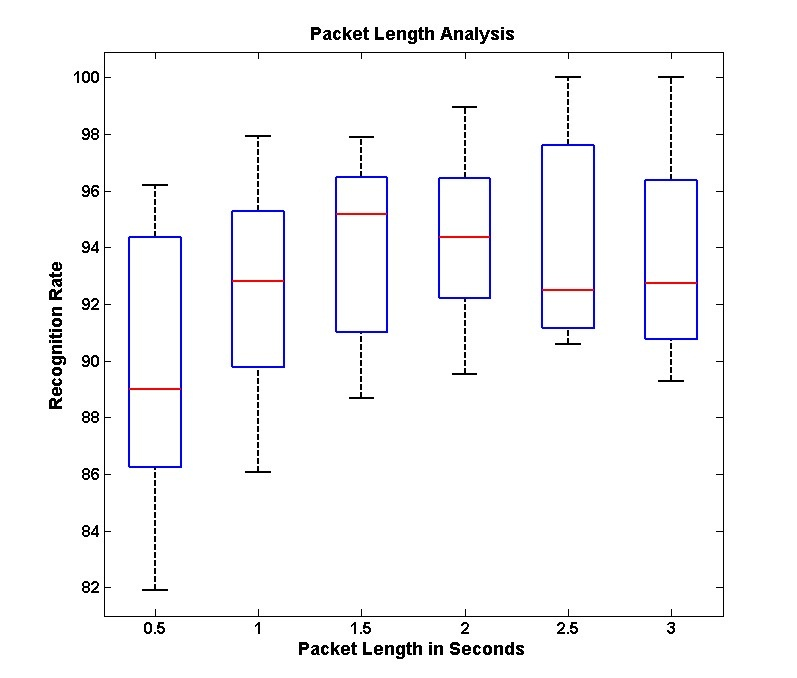
\includegraphics[width=4in]{PacketLength-Gentle.jpg}
\caption{Packet length to recognition rate comparison under the classic AdaBoost framework.}
\label{JMMFigure4}
\end{figure}

\begin{figure}
\centering
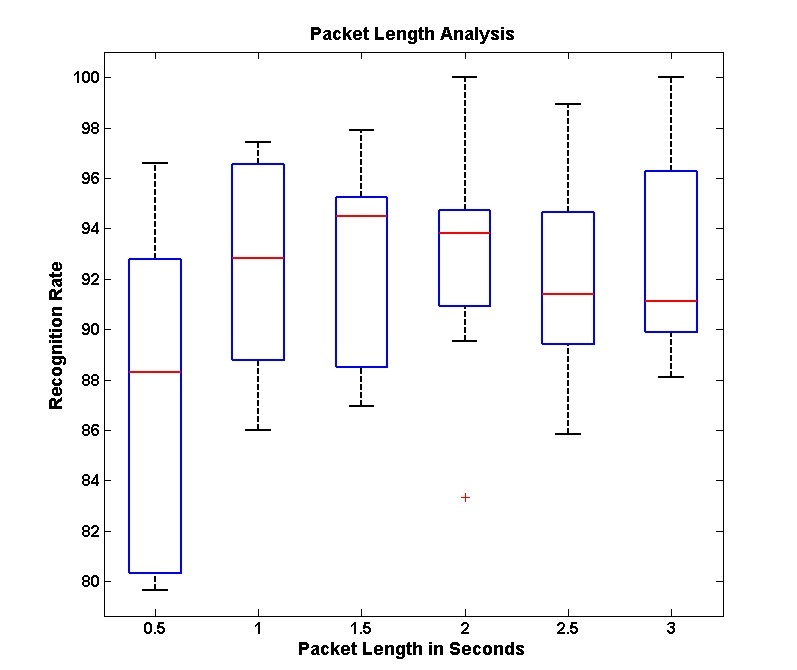
\includegraphics[width=4in]{PacketLength-Modest.jpg}
\caption{Packet length to recognition rate comparison under the Modest AdaBoost framework.}
\label{JMMFigure5}
\end{figure}


Table \ref{JMMTable3} presents the results from the experiment carried out to determine the generalization capabilities of the two classifiers. The entries in the table are counts as measured by the researchers of the number of false positives and false negatives counted manually while using the device for body rock detection and feedback. Five trails were carried out of 10 minutes each for determining these numbers. False positives represent the number of times the device falsely gave feedback when the user was not involved in rocking. It is important that this rate be minimal as too many false feedbacks would be discouraging for the user to continue using the assistive aid. The false negative represents the number of times the device did not detect that the user was rocking. This metric could be correlated to the failure of the device to perform its functional task.


\begin{table}
\centering
\begin{threeparttable}
\begin{tabular}{|l|c|c|}
  \hline
  % after \\: \hline or \cline{col1-col2} \cline{col3-col4} ...
  Generalization Capabilities & Classic AdaBoost & Modest AdaBoost \\
  \hline

  False Positives per Minute\tnote{1} & 86 & 44 \\
  False Negatives per Minute\tnote{1} & 20 & 9 \\
  \hline
\end{tabular}
\begin{tablenotes}\footnotesize
\item[1] Averaged over 10 minutes
\end{tablenotes}
\end{threeparttable}
\label{JMMTable3}
\end{table}

\begin{figure}
\centering
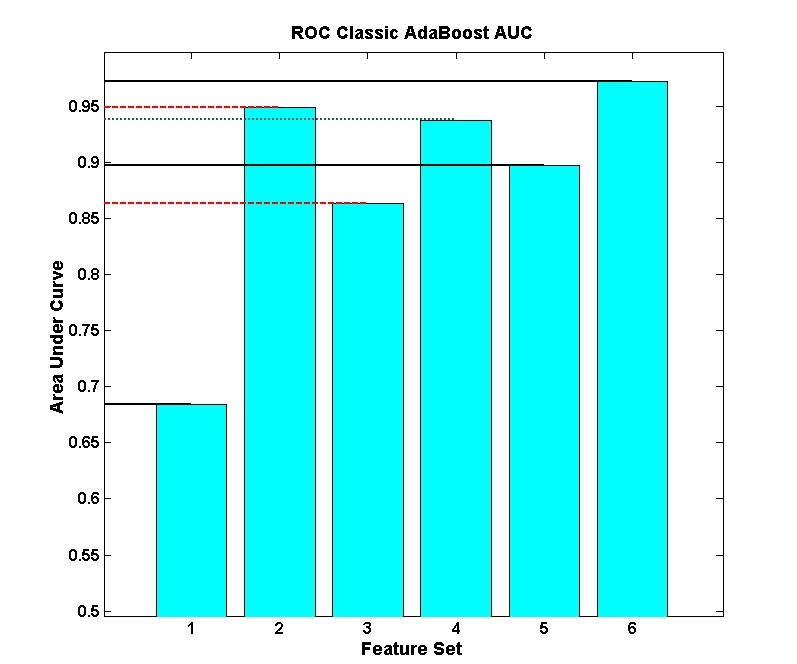
\includegraphics[width=4in]{AUCClassic.jpg} \\
(a)\\
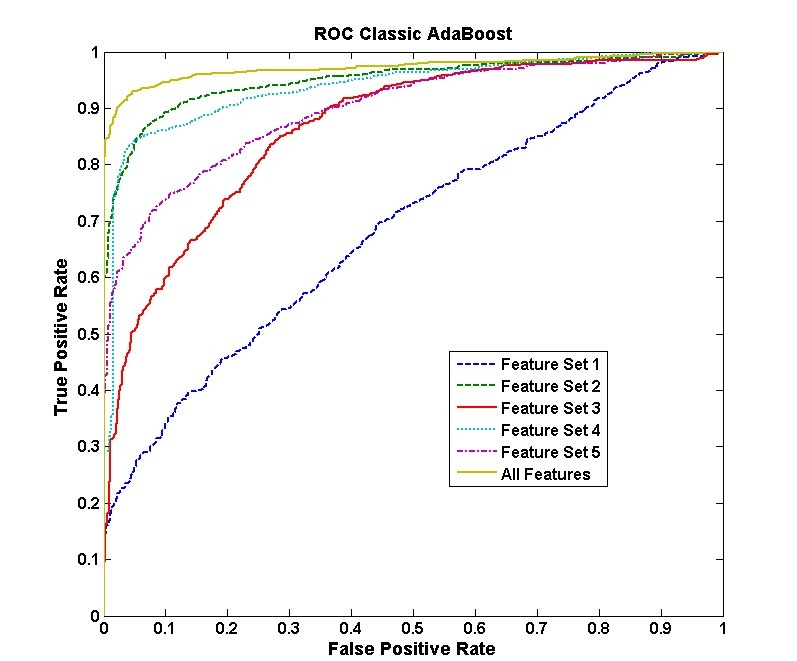
\includegraphics[width=4in]{ROC-Classic.jpg} \\
(b)
\end{figure}

\begin{figure}
\centering
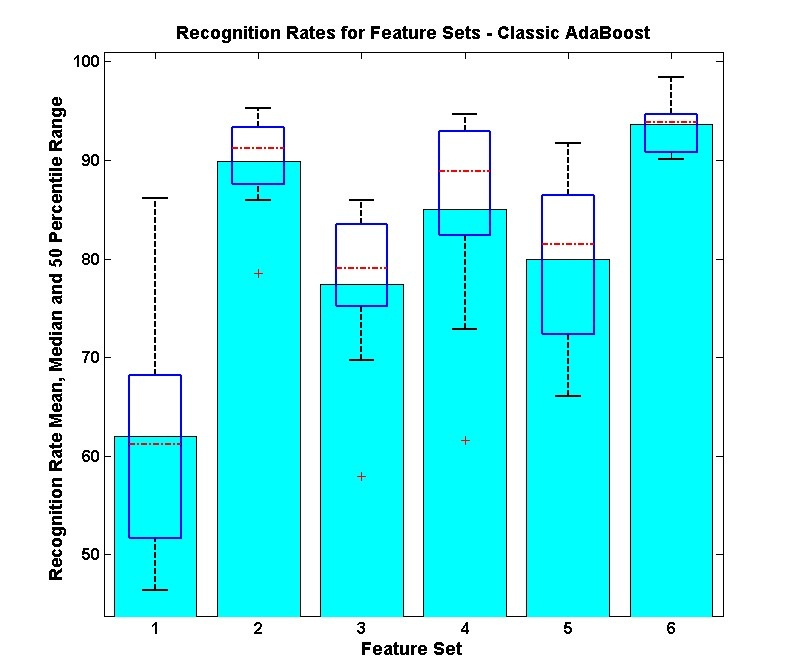
\includegraphics[width=4in]{FeatureSetRecogRate-Gentle.jpg}\\
(c)\\
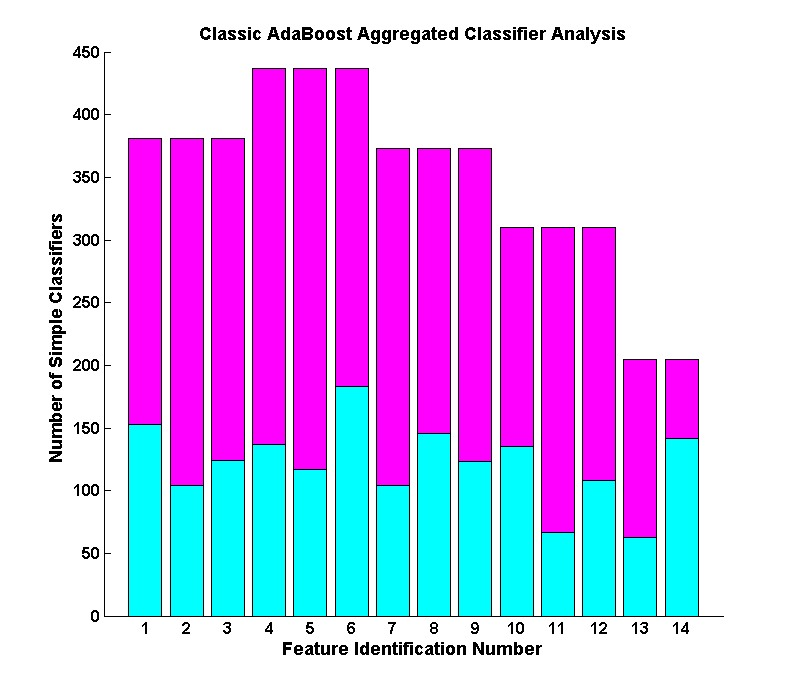
\includegraphics[width=4in]{ClassicClassifierAnalysis.jpg}\\
(d)
\caption{Piecewise performance analysis of the classic AdaBoost classifier framework; (a) Recognition rates under use of individual feature sets; (b) The Receiver Operating Characteristics (ROC) under the use of individual feature sets; (c) Area under the curve (AUC) for each feature set as estimated from the ROC; (d) The number of simple classifiers used by the aggregated AdaBoost classifier. Each set and each feature representation in the classifier pool are separately marked. In all the graphs Set 1 through 5 are as explained by Tables \ref{JMMTable1} and \ref{JMMTable2}. Set 6 represents a set containing all 14 features from Tables \ref{JMMTable1} and \ref{JMMTable2}.}
\label{JMMFigure7}
\end{figure}


\begin{figure}
\centering
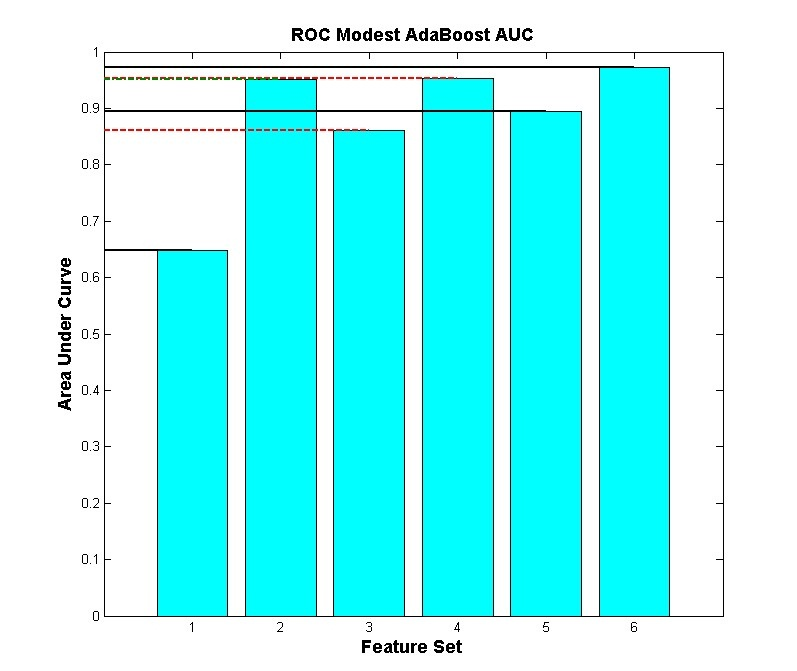
\includegraphics[width=4in]{AUCModest.jpg} \\
(a)\\
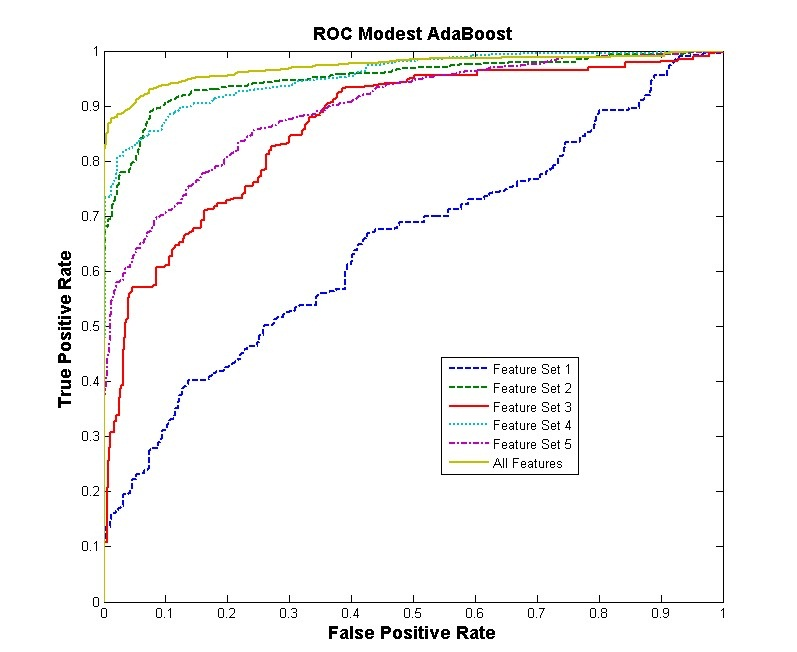
\includegraphics[width=4in]{ROC-Modest.jpg} \\
(b)
\end{figure}

\begin{figure}
\centering
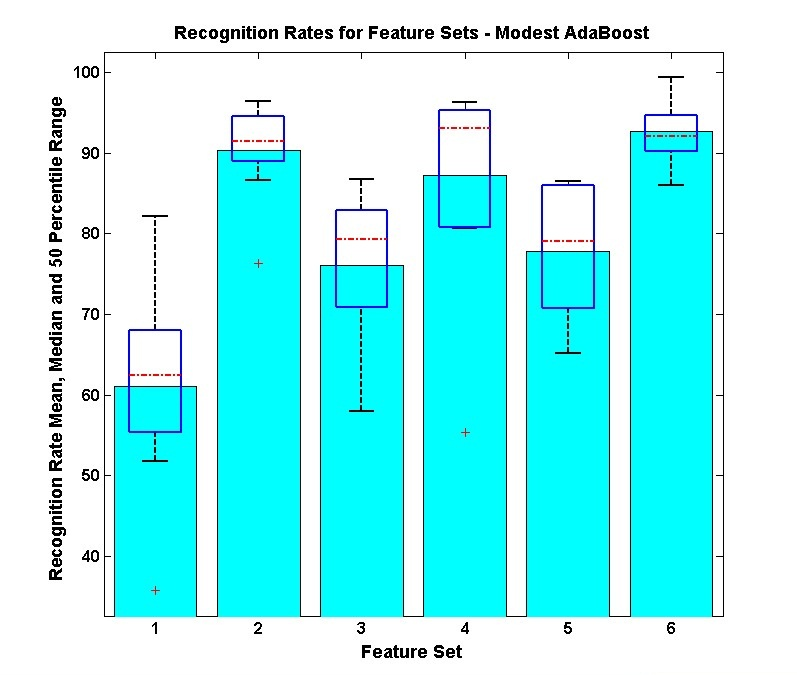
\includegraphics[width=4in]{FeatureSetRecogRate-Modest.jpg}\\
(c)\\
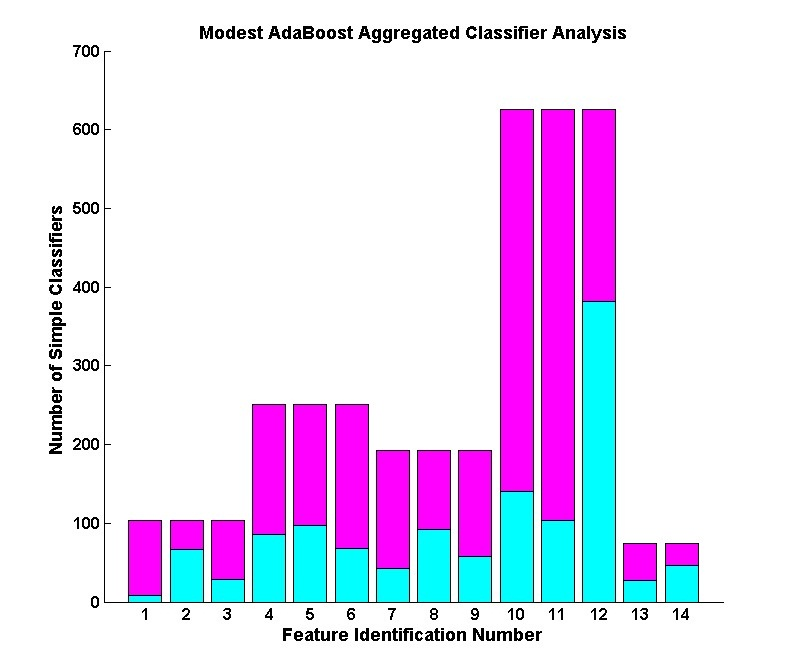
\includegraphics[width=4in]{ModestClassifierAnalysis.jpg}\\
(d)
\caption{Piecewise performance analysis of the classic AdaBoost framework; (a) Recognition rates under use of individual feature sets; (b) The Receiver Operating Characteristics (ROC) under the use of individual feature sets; (c) Area under the curve (AUC) for each feature set as estimated from the ROC; (d) The number of simple classifiers used by the aggregated AdaBoost classifier; Each set and each feature representation in the classifier pool are separately marked. In all the graphs Set 1 through 5 are as explained by Tables \ref{JMMTable1} and \ref{JMMTable2}. Set 6 represents a set containing all 14 features from Tables \ref{JMMTable1} and \ref{JMMTable2}.}
\label{JMMFigure8}
\end{figure}


Figure \ref{JMMFigure7} and Figure \ref{JMMFigure8} shows the piecewise analysis of the classic AdaBoost and Modest AdaBoost frameworks. Subfigure (a) shows the performance of each feature set considered one at a time in detecting body rocking; feature set 6 corresponds to the use of all 14 features together. For example, column 1 in Figure \ref{JMMFigure7}(a) represents the recognition performance using only temporal mean along x, y and z axis tested on all ten subjects. The bar graph in (a) shows the mean performance rate while the superimposed box plot shows the performance at first, second and third quartile as discussed earlier.

Subfigure (b) represents the Receiver Operating Characteristics (ROC) \cite{fawcett_introduction_2006} for the same six feature sets as in subfigure (a). ROC is plotted a false positive rate (FPR) versus true positive rate (TPR). The better the performance, the curve moves towards the (1,1) co-ordinate. For example, in Figure \ref{JMMFigure7}(b) Set 6 with all features is performing better than feature set 1 as Set 6 curve is closer towards (1,1) while the feature set 1 curve is almost along the diagonal of the plot. The diagonal of the ROC plot represents a recognition rate of 50\% i.e. random pick.

Subfigure (c) is a derivate of the ROC curves in subfigure (b). Each bar in the graph is representing the area under the corresponding curve (AUC) in (b). An area of 1 represents an ideal classifier with no false positive or false negatives, while an area of 0.5 represents randomness in the classifier output. AUC can be used to immediately determine the curve with the best performance.

Subfigure (d) is an understanding of how the aggregated AdaBoost classifier is built. As discussed above, AdaBoost classifier uses a collection of simple classifiers to achieve the final classifier. We plotted the number of times a particular feature is being used by the aggregate classifier. Further, the features are grouped into 5 sets corresponding to the five feature sets identified in Table 1. Columns belonging to the same set have the same top count which corresponds to the total simple classifiers used form that set. Each column within the set represents how many classifiers are used on each feature within that set. The count on the individual feature is represented by the bottom color along each column. For example, consider set 4 in Figure \ref{JMMFigure8}(d), features with identification number 10, 11 and 12 form this set (corresponding to the first order differential power from x, y and z axis of the accelerometer data) and have a top count of 646 simple classifiers. Within the group, the z axis differential power dominates the other two by having a count of 374.

\section{Discussion of Results}
Before discussing the results of the experiments conducted on the accelerometer data, we step back to the first research question that we identified in Section \ref{ResearchQuest}, Is there any evidence of individuals responding to rehabilitation for reducing stereotypic body rocking behavior? From the Psychology background work presented in Section \ref{BackGandRelatedWork}, we believe that there is enough evidence that individuals with sensory or cognitive impairment respond to rehabilitation through assistive devices. Specifically, the experiments highlighted in Section \ref{BandRWC} support the claim that body rocking can be decreased by providing immediate feedback to the individual.

Regarding the second research question, what is the state-of-the-art technology available to detect and notify individuals of their rocking behavior? We identified the state-of-the-art motion sensor that is small enough in form factor to become part of one's everyday clothing. Further, we designed this device to be discrete so that the user does not feel any intrusion into their everyday activities. The software can be run on any mobile processing device that the user already carries like a cell phone or PDA. This allows the users to use the device without carrying any additional load. Our solution to this research question caters to the Acceptance design dimension that we identified in Section \ref{BandRWC} 1.

Focusing on the third research question, Is it possible to build a device that detects body rocking condition and how well can it distinguish body rocking from other functional activities of daily living? We turn our attention to the various results presented in Section \ref{ResultsJMM} to prove the efficiency of our proposed method in detecting body rocking and distinguishing it from other non-rocking behavior.

\subsection{Packet Length, and Detection Efficiency}
From Figure \ref{JMMFigure4} and Figure \ref{JMMFigure8}, it is evident that the recognition rates for the two classifiers are comparable and the median recognition rate ranges from 89\% to 95\%. Based on these numbers, the best performance was achieved at a sample length of 1.5 seconds or 150 samples per packet. Packet length of 150 samples has the highest recognition rate on both the classifiers. Comparing this packet with the 2 seconds packet length or 200 samples per packet, we notice that the 2 seconds packet is very close behind and it has a smaller 1.5 IQR box. Thus, the variance in the recognition rates between 10 subjects is lesser in the 200 samples packet length, implying that the results are more consistent. Further, we noticed that the average natural rocking motion of the 10 subjects was around 27 rocks a minute (i.e. 27 rocks in 60 seconds or 2.22 seconds per rock; this is supported by results from \cite{newell_variability_1999}), which implies that a latency of 2 seconds was the closest to the time duration of a single rocking action. As mentioned earlier, all experiments were carried out with an overlap 0.5 seconds or 50 samples between successive packets. Combing these two results, we have

\begin{enumerate}
\item \emph{Optimum Packet Length}
2 seconds or 200 samples with 0.5 seconds or 50 samples overlap between packets.
\item \emph{Best Detection Rate}
@ 2 seconds packet length $\approx$ 94\% under both classifiers
\end{enumerate}

\subsection{Generalization Capabilities}
From Figure \ref{JMMFigure4} and Figure \ref{JMMFigure8}, it is very difficult to distinguish any performance benefits between classic AdaBoost and Modest AdaBoost. But analyzing Table \ref{JMMTable3}, we can notice a dramatic difference in the performance of the Modest AdaBoost when compared to classic AdaBoost. The number of false positives is down from 86 to 44 over a ten minute period. That is, the user receives nearly half less number of false feedback with Modest AdaBoost framework when compared to the classic AdaBoost. This was not evident in the detection tests that were carried out with data collected from Routine C (Section IV - A 3.). We asked the question of why there is an increased performance in Modest AdaBoost and why there is a discrepancy between the test results from Routine C and the naturalistic data capture (Section \ref{RountineC}). The answer to these questions lies in the generalization capabilities of the two classifiers. We noticed that most of the false feedback provided by classic AdaBoost occurred while the user was sitting and not rocking. In hind sight, we realized a slight discrepancy in our non-rocking (negative class) data collection. While capturing data under Routine B (as explained in Section \ref{RoutineB}) the participants were asked to perform various tasks that did not involve rocking to use as negative training set. We realized that most of the participants performed tasks that involved some form of walking or standing activities while they did no activity that involved sitting and not rocking. Thus, just sitting activity was a non-rocking event that was not represented in the training data set. We hypothesize that classic AdaBoost over trained on the non-rocking data while Modest AdaBoost, which is penalized for learning the training set very well, had a better generalization. Extending this heuristic analysis to a more formal analysis, we look at the piecewise performance of the two classifiers. Comparing the ROC curves from Figure \ref{JMMFigure7} (b) with Figure  \ref{JMMFigure8} (b), it can be seen that feature set 2 - Variance and feature set 4 - First Order Differential Power performed the best following Set 2 - All features set. Now comparing Figure  \ref{JMMFigure7} (d) with Figure  \ref{JMMFigure8} (d) it can be seen that Modest AdaBoost distributed it simple classifiers such that there were more classifiers representing the two feature sets 2 and 4. On the other hand, the classic AdaBoost's distribution of simple classifiers is unexplainable as feature set 1 - Mean - seems to have received more representation than set 4. Mean had the worst performance as an individual feature set as can be verified by the ROC curve that comes closest to the diagonal on the plot hinting that the performance is barely above random guess. Contrasting this with Modest AdaBoost selection, Mean is in the bottom two sets among the five feature sets. This bad performance of Mean as a feature set can be understood by looking at the graph shown in the first row and last column of Table 1. It can be seen that the Mean acceleration values between rocking and non-rocking are not significantly different. Table \ref{JMMTable1} Row 2 and Table \ref{JMMTable2} Row 1 highlights the capabilities of Variance and First Order Differential Power in distinguishing rocking from non-rocking. This is further confirmed by the ROC graph.


Feature 4 having the highest distribution of simple classifiers under Modest AdaBoost (Figure  \ref{JMMFigure8} (d)), within this feature set we can see that the highest number of simple classifier is assigned to feature 12 which corresponds to First Order Differential Power on z axis. As can be verified from Figure \ref{JMMFigure3}, the best distinguishing character between non-rocking and rocking patterns seems to be the transformation of a random signal pattern on z-axis to a deterministic sinusoidal waveform. If this can be the true identity of the rocking data stream, feature 12 would capture it in the best possible manner by measuring the power in the first order differential of the temporal signal. Using this feature as the most reliant feature would provide a good basis to support the final classifier selected by Modest AdaBoost.


We are now ready to answer the last research question stating that the use of approximately 2 seconds (or 200 samples @ 100 Hz sampling rate) packet length used with a learning framework biased towards generalized learning (like Modest AdaBoost) would be a good assistive technology solution for detecting and giving feedback towards stereotypic body rocking. We can extend the same argument to other body mannerisms that involve any form of repetitive body part movement.

\section{Conclusion}
 In this chapter, we have addressed the topic detecting stereotypic body mannerisms, specifically body rocking, and propose a technology solution for providing an assistive technology that may reduce or control body rocking. We have discussed the hardware and software components of the proposed system in detail and offer a thorough analysis on the learning framework that provides generalization benefits to allow this framework to be extended to detection of any body mannerism. Investigations are in progress to determine how incoming samples of acceleration data can be labeled automatically by the system based on the AdaBoost classifier's classification confidence metrics. This would provide opportunity for self-learning \cite{raina_self-taught_2007} modes where the device can readily understand and learn data points that were not available in the training set. Combining such self-learning into a generalized learner would provide immense opportunities for not only body mannerism detection, but for solving future data mining problems where typical lab setting training data collection would just not be sufficient to train a robust classifier.

From the assistive technology perspective, we plan to integrate a well planned self-monitoring as a part of the proposed device. We are exploring the broad area of human communication to determine the best cognitive self-correction techniques that could augment the proposed solution. . We have implemented a rudimentary form of real-time body rock counter, as discussed in [3], but we have not yet tested it for its feedback capabilities.


\chapter{PERSON-SPECIFIC FACE RECOGNITION}
face recognition has the potential for recognizing
people at a distance, without their knowledge or cooperation.  For
decades, banking, retail, commercial, and industrial buildings have
been populated with surveillance cameras that capture video streams
of all people passing through critical areas.  More recently, as a
result of threats to public safety, some public places (such as in
Glasgow and London) have been heavily populated with video
surveillance cameras.  On average, a person moving through London is
captured on video over 5 times a day. This offers an unprecedented
basis for developing and testing face recognition as a biometric for
security and surveillance.

Given this great potential, it is not surprising that many private
corporations have attempted to develop and deploy face recognition
systems, as an adjunct to existing video security and surveillance
systems.  However, the performance of these systems has been
disappointing. Depending on how such a system is adjusted,
miscreants might easily pass through the system undetected, or
innocent people might be incessantly inconvenienced by false alarms.

One of the most difficult problems that face recognition researchers
encounter in surveillance applications is that face databases of
miscreants typically contain only frontal and profile views of each
person's face, with no intermediate views.  Surveillance videos
captured of the same person with the same camera in the same
lighting conditions might have face images that look quite
different, due to pose angle variations, making it very difficult to
compare captured face images to those in a database.  Combine this
problem with the fact that miscreants are highly motivated to
disguise their identity, and the fact that face databases often
contains thousands of faces, and the problem seems insurmountable.

Given all of these complicating factors, it is premature to rely
upon face recognition systems for detecting miscreants in public
places.  On the other hand, the use of face recognition in
controlled access applications (where users are highly motivated to
cooperate, and where face database images can be both captured and
tested with the same camera under the same illumination conditions)
is certainly within the limitations of current face recognition
algorithms.

\subsection{Employing face recognition to facilitate social interactions}
However, there is a real-world application for face recognition that
is moderately challenging, but still potentially within the realm of
possibility. When people who are blind enter a room, they might find
it awkward to initiate social interactions because they don't know
how many people are in the room, who those people are, or where they
are standing. A robust, wearable
face recognition device could solve this problem.

This problem is simplified considerably by the fact that, on a
day-to-day basis most people encounter a limited number of people
whom they need to recognize.  It is further simplified by the fact
that people typically don't attempt to disguise their appearance in
social situations.  When a new person is encountered, the system
could employ face detection to extract and save a sequence of face
images captured during a conversation.  This would provide a wide
variety of facial expressions and pose angles, that could be stored
in a database, and used for training a face recognition algorithm.

As people use such an assistive device over an extended period of
time, they will learn both its abilities and its limitations.
Conjectural information from the system can then be combined with
the user's other sensory abilities (especially hearing) to jointly
ascertain the identity of the person.  This synergy between the user
and the system relaxes some of the stringent requirements normally
placed on face recognition systems.

However, such an assistive technology application still poses some
significant challenges for researchers.  One problem is the extreme
variety of in lighting conditions encountered during normal daily
activities. While there are standards for indoor office lighting
that tend to provide diffuse and adequate lighting, lighting in
other public places might vary considerably. For example, large
windows can significantly alter lighting conditions, and
incandescent lighting is much more yellow than florescent lighting.
Outdoor lighting can be quite harsh in full sunlight, and much more
blue and diffuse in shadows. A person who is blind might not be
aware of extreme lighting conditions, so the system would need to
either (1) be tolerant of extreme variations or (2) recruit the user
to ameliorate those extreme conditions.

In summary, the development of an assistive face recognition system
for people who are blind provides a more tractable problem for face
recognition researchers than security and surveillance applications.
It imposes a somewhat less stringent set of requirements because (1)
the number of people to be recognized is generally smaller, (2)
facial disguise is not a serious concern, (3) multiple pose angles
and facial expressions of a person can be captured as training
images, and (4) the person recognition process can be  a
collaborative process between the system and the user.

In an attempt to provide such an assistive face recognition system,
we have developed a new methodology for face recognition that
detects and extracts unique features on a person's face, and then
uses those features to recognize that person. Contrast this with
conventional face recognition algorithms that might avoid the use of
a few distinguishing features because that approach might make the
system very vulnerable to disguise.

\section{Face Recognition in Humans}
For decades, scientists in various research areas have studied how
humans recognize faces. Developmental psychologists have studied how
human infants start to recognize faces, cognitive psychologists have
studied how adolescents and adults perform face recognition;
neuroscientists have studied the visual pathways and cortical
regions used for recognizing faces, and neuropsychologists have
attempted to integrate knowledge from neurobiological studies with
face recognition research. Computer vision researchers are
relatively new to this area, and have attempted to develop face
recognition algorithms using image processing methods.  Only
recently have computer vision researchers been motivated to better
understand the process by which humans recognize faces, in order to
use that knowledge to develop robust computational models. Their new
interest has lead to more inter-disciplinary face recognition
research, which will likely aid our understanding of face
recognition.

New studies have shown that humans, to a large extent, rely on both
the featural and configural information in face images to recognize
faces ~\cite{Schw2003}. Featural information provides details about
the various facial features, such as the shape and size of the nose,
the eyes, and the chin.  Configural information defines the
locations of the facial features, with respect to each other.
Psychologists Vicki Bruce and Andrew Young ~\cite{Bruce2006} agree
with this dual representation, saying that humans create a
view-centric description of a human face by relying upon
feature-by-feature perceptual input, which is then combined into a
structural model of the face.

Sadar et al ~\cite{Sadr2003} showed that characteristic facial
features are important for recognizing famous faces. For example,
when they erased eye-brows from famous people's faces, face
recognition by human participants was adversely affected.  Young
~\cite{Young1987} showed that human participants were confused when
asked to recognize faces that combined facial features from
different famous faces. These studies suggest that the details of
facial features are important in the recognition of faces.

However, ~\cite{Sinha2006} showed that the relative locations of the
facial features was also very important for the recognition of
faces.  They collected face images of famous personalities, and then
changed the aspect ratio of those images, such that the height was
greatly compressed, while the width was emphasized.  Surprisingly,
all the resulting face images were still recognizable, despite their
contorted appearance, as long as the relative locations of the
features were maintained within the distorted image.  This study
suggests that humans can flexibly use the configural information
when recognizing faces.

Another important area of research in the human perception of faces
has been in understanding the medical condition of face blindness,
called \emph{prosopagnosia}.  People with prosopagnosia are unable to
recognize faces including their own. Until recently it was assumed
that prosopagnosia was acquired often as a result of a localized
stroke. However new evidence suggests that a substantial portion of
the general population have a congenital form of prosopagnosia
~\cite{Mccon1976}. Kennerknecht et al ~\cite{Kenner2006} conducted a
survey of 789 students in 2006 which showed that 17 (2.5\%) suffered
from congenital prosopagnosia. These students went about their daily
life without realizing their disorder in face recognition.

Other studies at the Perception research centers at Harvard and Univ
College of London have shown that prosopagnosics recognize people
using unique personal characteristics, such as hair style, gait,
clothing, and voice. These findings suggest that the detection of
unique personal characteristics might provide a basis for face
recognition systems to better recognize people. Since current
methods of face recognition have met with only limited success, it
makes sense to explore the use of this alternative approach.

Research in Own-Race Bias (ORB) in face recognition ~\cite{Turk2005}
has also revealed some interesting results regarding human face
recognition capabilities. David Turk et al. found that, when humans
are presented with new objects or new faces, they initially learn to
recognize those objects and faces based on their distinctive
features.  Then, as familiarity increases, they incorporate
configural information, moving towards holistic recognition. This
study suggests that distinctive features are important during the
initial stages of face recognition, and that configural information
subsequently provides additional useful information.

Distinctive facial features can take many different forms.  For
example, after a first encounter with a person who has a handlebar
moustache, we readily recognize that person by the presence of his
distinctive feature.  Similarly, a person with a large black mole on
her face will be remembered by first-time acquaintances by that
feature.  Given the current limited understanding of how humans
recognize faces, it makes sense to use these observations as the
basis for a new approach to face recognition.

The research described in this chapter is based on the approach of
identifying distinctive facial features that can be used to
distinguish each person's face from other faces in a face database.
In recognition of the role played by configural information in the
later stages of face recognition, it also takes into account the
location of these features with respect to each other.  The results
of our research suggest that this approach can be very effective for
distinguishing one person's face from other faces.

\section{Our Approach to Face Recognition}
Having introduced the potential for using characteristic
person-specific features for face recognition, we now turn our
attention towards the development of a method for discovering such
features, and for using them to index face images. Then we propose a
novel methodology for face recognition, using person-specific
feature extraction and representation. For each person in a face
database, a learning algorithm discovers a set of distinguishing
features (each feature consisting of a unique local image
characteristic, and a corresponding face location) that are unique
to that person. This set of characteristic facial features can then
be compared to the normalized face image of any person, to determine
the presence or absence of those features. Because a unique set of
features is used to identify each person in the database, this
method effectively employs a different feature space for each
person, unlike other face recognition algorithms that assign all of
the face images in the database to a locality in a shared feature
space. Face recognition is then accomplished by a sequence of steps,
in which  query face images is mapped into a locality within the
feature space of each person in the database, and its position is
compared to the cluster of points in that space that represents that
person. The feature space in which the query face images are closest
to the cluster is used to identify the query face images.

Having introduced the conceptual theory behind a person-specific
characteristic feature extraction approach to face recognition, we
now propose in the subsequent sections a method for detecting and
extracting such features from face images, and for constructing a
feature space that is unique to each person in the database.

\section{Feature Extractors}
\subsection{What is a Feature?}
The task of face recognition is inherently a multi-class
classification problem. For every face image $X$, there is an
associated label $y$ that is the name of the class, i.e. the name of
the person depicted in the image. While $X$ represents the image of
the person, there is no inherent constraint on whether the image is
a color RGB, HUV or YCbCr image, or a gray-scale image with a
gray-scale range of 0 to 255, or even spectral representation that
is extracted from the face image using Fourier transform or
Wavelets. Irrespective of the image representation, the basis
vectors spanning that representation are called features. The
feature space spanned by these basis vectors is partitioned  by the
decision boundaries that ultimately define the different classes in
the multi-class problem of face recognition. In this work, we choose
a particular set Gabor filters as feature detectors, and each of
those feature detectors for each person in the database, and that
set of Gabor filters spans a unique feature space for that person.

\subsection{Gabor Features}
\label{subsecGF} Gabor filters are a family of functions (sometimes
called Gabor Wavelets) that are derived from a mother kernel (a
Gabor Function) by varying the parameters of the kernel. As with any
wavelet filters, the Gabor filters extract local spatial frequency
content from the underlying image. Gabor Filters specifically
capture the spatial location and spatial orientation of the
intensity variations in the image underneath the filter's location.
By varying the spatial frequency and the spatial scope of the
filters, it is possible to extract a Gabor coefficient that
partially describes the nature of the image underneath it. The
coefficients obtained by filtering a locality in a face image with a
set of different Gabor Filters are called Gabor Features.

\subsubsection{Use of Gabor Filters in Face Recognition}
Gabor filters have been widely used to represent the receptive field
sensitivity of simple cell feature detectors in the human primary
visual cortex. Recognizing this fact, Gabor features have been
widely used by face recognition researchers. Over the last few
years, the extensive use of Gabor wavelets as generators of feature
spaces for face recognition, has led to objective studies of the
strength of Gabor features for this application. For example, Shan
et al [Shan2004] reviewed the strength of Gabor features for face
recognition using an evaluation method that combined both alignment
precision and recognition accuracy. Their experiments confirmed that
Gabor features are robust to image variations caused by the
imprecision of facial feature localization. As indicated by G�kberk
et al ~\cite{Gokberk2007}, several studies have concentrated on
examining the importance of the Gabor kernel parameters for face
analysis. These include: the weighting of Gabor kernel-based
features using the simplex algorithm for face recognition
~\cite{Wiskott1997}, the extraction of facial subgraphs for head
pose estimation ~\cite{Kruger1997}, the analysis of Gabor kernels
using univariate statistical techniques for discriminative region
finding ~\cite{Kalocsai2000}, the weighting of elastic graph nodes
using quadratic optimization for authentication ~\cite{Tefas2001},
the use of principal component analysis (PCA) to determine the
importance of Gabor features ~\cite{Liu2004}, boosting Gabor
features ~\cite{Yang2004} and Gabor frequency/orientation selection
using genetic algorithms ~\cite{ Wang2002}.

 A relevant work on Gabor Filters for face recognition that is closely related to the
research presented here is by Wiskott and von der Malsburg
~\cite{wiskott_face_1997}. Their work
~\cite{von_der_malsburg_nervous_1985}
~\cite{bienenstock_neural_1987} ~\cite{wiskott_face_1995}
~\cite{wiskott_face_1996},~\cite{wiskott_face_1997} proposes a
framework for face recognition that is based on modeling human face
images as labeled graph. Termed {\em Elastic Bunch Graph Matching}
(EBGM), the technique has become a cornerstone in face recognition
research. Each node of the graph is represented by a group of Gabor
filters/wavelets (called "jets") which are used to model the
 intensity variations around their locations. The edges
of the graph are used to model the relative location of the various
jets. Since the jets represent the underlying image characteristics,
it is desirable to place them on fiducial points on the face. This
is achieved by {\em manually} marking the locations of the facial
fiducial points using a small set of controlled graphs that
represent ``general face knowledge'', which represents an average
geometry for the human face. In our work, a genetic algorithm is
used to obtain the spatial location of the fiducial points. Besides
automating the process of locating these points, our work identifies
spatial locations on the face image that are unique to every single
person, rather than relying on an average geometry.

Closely following the work of Wiskott et. al., Lyons et. al.
~\cite{lyons_automatic_1999} proposed a technique that uses Gabor
Filter coefficients extracted at 1) automatically located
rectangular grid points or 2) manually selected image feature
points. These coefficients are then used to bin face images based on
sex, race and expression. The technique relies on a combined
Principal Component Analysis (PCA) dimensionality reduction and
Linear Discriminant Analysis (LDA) classification over the extracted
Gabor coefficients, to achieve a pooling of images. While the
classification task is not related directly to {\em identifying}
individuals from face images, this technique also demonstrates the
ability of Gabor Filters to extract features that can encode subtle
variations on facial images, providing a basis for face
identification.

\subsubsection{Gabor Filters}
Mathematically, Gabor Filters can be defined as follows:
\begin{equation}
\Psi_{\omega,\theta}  \left(x,y\right) =
\frac{1}{2\pi\sigma_x\sigma_y}\cdot G_\theta\left( x,y\right)\cdot
S_{\omega,\theta}\left(x,y\right) \label{Eqn:GF}
\end{equation}
\begin{equation}
G_\theta\left( x,y\right) = \exp \left\{ - \left( \frac{\left(x \cos
\theta + y \sin \theta \right)^2}{2\sigma_x^2}+\frac{\left(-x \sin
\theta + y \cos \theta \right)^2}{2\sigma_y^2}\right)\right\}
\label{Eqn:G}
\end{equation}
\begin{equation}
S_{\omega,\theta}\left(x,y\right) = \left[\exp \left\{i\left(\omega
x \cos \theta + \omega y \sin \theta \right)\right\} - \exp \left\{-
\frac{\omega^2 \sigma^2}{2} \right\}\right] \label{Eqn:S}
\end{equation}

where,
\begin{itemize}
\item $G_\theta\left( x,y\right)$ represents a Gaussian Function.
\item $S_{\omega,\theta}\left(x,y\right)$ represents a Sinusoid Function.
\item $\left(x,y\right)$ is the spatial location where the filter is centered with respect to the image axis.
\item $\omega$ is the frequency parameter of a 2D Sinusoid.
\item $\sigma^2_{dir}$ represents the variance of the Gaussian (and thus the filter) along the specified direction.
$dir$ can either be $x$ or $y$. The variance controls the region
around the center where the filter has influence.
\end{itemize}

From the definition of Gabor filters, as given in Equation
\ref{Eqn:GF}, it is seen that the filters are generated by
multiplying two components: a Gaussian Function $G_\theta\left(
x,y\right)$ (Equation \ref{Eqn:G}) and a Sinusoid
$S_{\omega,\theta}\left(x,y\right)$ (Equation \ref{Eqn:S}). The
following discussions detail the two components of Equation
\ref{Eqn:GF}.

\subsubsection{Gaussian Function}
The 2D Gaussian function defines the spatial spread of the Gabor
filter. This spread is defined by the variance parameters of the
Gaussian, along the $x$ and $y$ direction together with the
orientation parameter $\theta$. Figure \ref{Fig:G}(a) shows a 3D
representation of the Gaussian mask generated with $\sigma_x = 10$
and $\sigma_y = 15$ and rotation angle $\theta = 0$. The image in
Figure \ref{Fig:G}(b) shows the region of spatial influence of an
elliptical mask on an image, where the variance in the $x$ direction
is larger than the variance in the $y$ direction.

\begin{figure}
\begin{center}
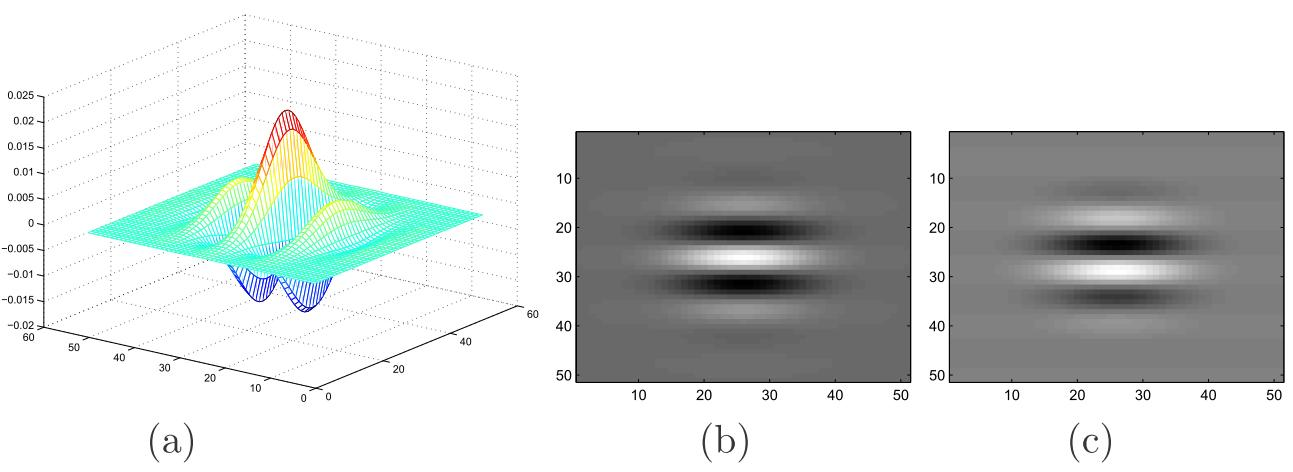
\includegraphics [width=5.5in] {FRFig1.JPG}
\caption{(a) 3D representation of a Gaussian
mask; $\sigma_x = 10$, $\sigma_y = 15$ and $\theta=0$
\newline (b)Image of the Gaussian mask $\sigma_x = 10$, $\sigma_y
= 15$ and $\theta=0$}
\label{Fig:G}
\end{center}
\end{figure}


Typically the Gaussian filter has the same variance along both the
$x$ and $y$ directions, that is $\sigma_x = \sigma_y = \sigma$.
Under such conditions the rotation parameter $\theta$ does not play
any role as the spread will be circular.

\subsubsection{Sinusoid}
The 2D complex Sinusoid defined by Equation \ref{Eqn:S} generates
the two Sinusoidal components of the Gabor filters which (when
applied to an image) extracts the local frequency content of the
intensity variations in the signal. The complex Sinusoid has two
components (the real and the imaginary parts) which are two 2D
sinusoids that are phase shifted by $\frac{\pi}{2}$ radians. Figure
\ref{Fig:CS}(a) shows the 3D representation of a Sinusoidal signal
(either real or imaginary) at $\omega = 0.554$ radians and $\theta =
0$ radians, while Figure \ref{Fig:CS}(b) and \ref{Fig:CS}(c) show an
image of the real and imaginary parts of the same complex Sinusoid,
respectively. It can be seen that the two filters are similar,
except for the $\pi$ radian phase shift.

\begin{figure}
\begin{center}
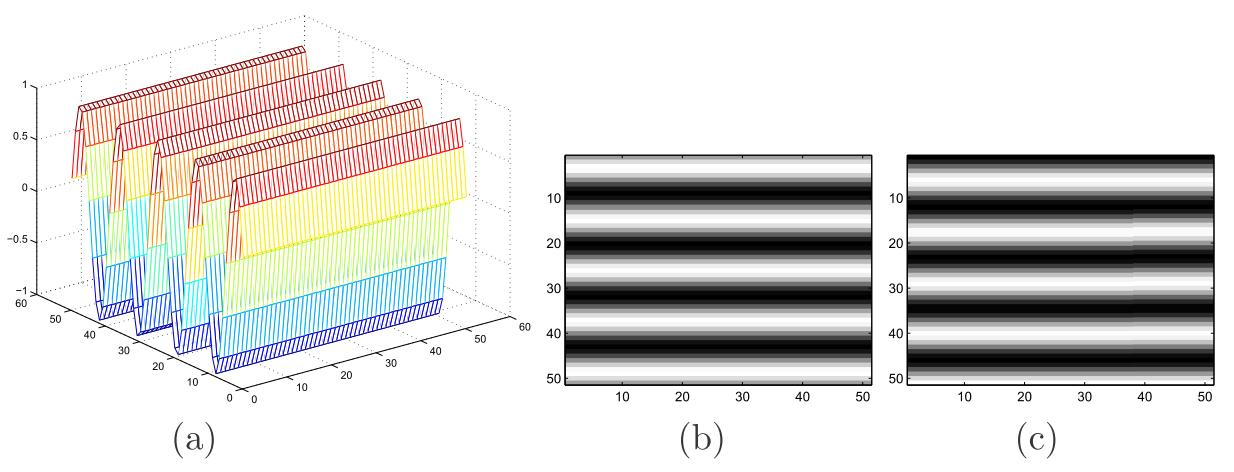
\includegraphics [width=5.5in] {FRFig2.JPG}
\caption{(a)3D representation of a Sinusoid $S_{\omega,\theta}$
\newline (b)Image representation of the real part of the complex
Sinusoid $\Re\left\{S_{\omega,\theta}\right\}$\newline (c)Image
representation of the imaginary part of complex Sinusoid
$\Im\left\{S_{\omega,\theta}\right\}$} \label{Fig:CS}
\end{center}
\end{figure}

Multiplying the Gaussian and the sinusoid generates the complex
Gabor filter, as defined in Equation \ref{Eqn:GF}. If
$\sigma_x=\sigma_y=\sigma$, then the real and imaginary parts of
this complex filter can be described as follows.

\begin{equation}
\Re\left\{\Psi_{\omega,\theta}  \left(x,y\right) \right\} =
\frac{1}{2\pi\sigma^2}\cdot G_\theta\left( x,y\right)\cdot
\Re\left\{S_{\omega,\theta}\left(x,y\right)\right\}
\end{equation}

\begin{equation}
\Im\left\{\Psi_{\omega,\theta}  \left(x,y\right) \right\} =
\frac{1}{2\pi\sigma^2}\cdot G_\theta\left( x,y\right)\cdot
\Im\left\{S_{\omega,\theta}\left(x,y\right)\right\}
\end{equation}

Figure \ref{Fig:GF}(a) shows the 3D representation of a Gabor filter
(either real or imaginary) at $\omega = 0.554$ radians, $\theta = 0$
radians, and $\sigma = 10$ and Figure \ref{Fig:GF}(b) and
\ref{Fig:GF}(c) show an image with the real and imaginary parts of
the complex filter.

\begin{figure}
\begin{center}
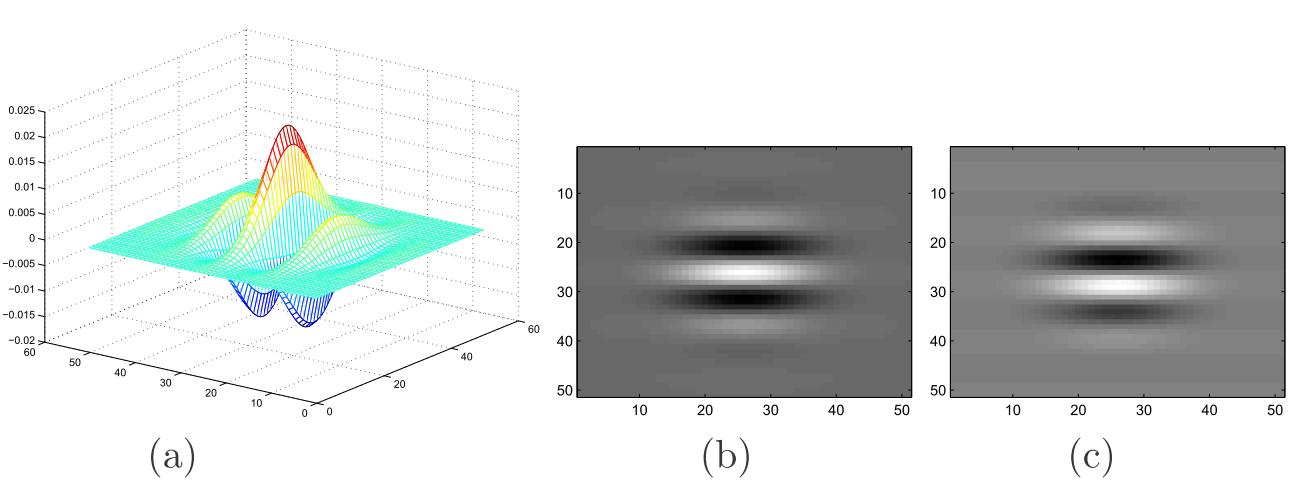
\includegraphics [width = 5.5in] {FRFig3.JPG}
\caption{(a)3D representation of a Gabor filter
$\Psi_{\omega,\theta}$ \newline (b)Image representation of the real
part of Gabor filter  $\Re\left\{\Psi_{\omega,\theta}\right\}$
\newline (c)Image representation of the imaginary part of Gabor filter
$\Im\left\{\Psi_{\omega,\theta}\right\}$} \label{Fig:GF}
\end{center}

\end{figure}

In order to extract a Gabor feature at a location $\left(x,y\right)$
of an image $I$, the real and imaginary parts of the filter are
applied separately to the same location in the image, and a
magnitude is computed from the two results. Thus, the Gabor filter
coefficient at a location $\left(x,y\right)$ in an image $I$ with a
Gabor filter $\Psi_{\omega,\theta}$ is given by
\begin{equation}
C_{\Psi}\left(x,y\right) = \sqrt{\left(I \left(x,y\right) *
\Re\left\{\Psi_{\omega,\theta}\left(x,y\right)\right\}\right)^2 +
\left(I \left(x,y\right) *
\Im\left\{\Psi_{\omega,\theta}\left(x,y\right)\right\}\right)^2}
\label{Eqn:GaborCoeff}
\end{equation}

In our experiments, a \emph{Gabor filter bank} was created by varying
three parameters of $\Psi_{\omega,\theta}$: (1) the frequency
parameter $\omega$, (2) the orientation parameter $\theta$, and (3)
the variance parameter $\sigma$. We chose five values for each of
these parameters thereby generating 125 different Gabor filters.

\begin{itemize}
\item $\omega = \left(2^{(-f+2)/2}\cdot \pi\right)$ where, $f =
\{0, 1, 2, 3, 4\}$ \item $\theta = \left(\frac{\pi}{2} \cdot \frac
{1} {5} \cdot t \right)$ where, $t = \{0, 1.25, 2.5, 3.75, 5\}$
\item $\sigma = \{5, 10, 15, 20, 25\}$
\end{itemize}

\section{The Learning Algorithm}
The proposed method uses the above described Gabor filters to find
distinguishing features (and corresponding feature locations) within
a face image. That is, for each person in the database, the
algorithm finds a set of Gabor filters which, when applied at their
corresponding $(x,y)$ locations within the image will produce
coefficients that are unique for that individual. This means that
all of the 125 Gabor filters in the filter bank are applied at each
and every location of each of the individual's face images, and then
tested for their ability to distinguish every individual. Given a
$128 \times 128$ face image, there will be $128 \times 128 \times
125 \times n$ filter coefficients that will be generated per face
image per person, where $n$ is the number of characteristic features
to be extracted for each person. This must be computed for every
person in the training set, which further increases the search
space. To search such a vast space of parameter values (the size of
the Gaussian mask, the frequency of the complex sinusoid, the
orientation of the entire Gabor filter, and the $(x,y)$ location
where the filter is placed) it is important that some scheme for
effective search be incorporated into the system. To this end, we
have chosen Genetic Algorithms to conduct the search. For each
person in the training set, all of the face images that depict to
that person are indexed as positives, while all of the other face
images in the database are indexed as negatives. Dedicated Genetic
Algorithm based search is conducted with these positive and negative
images, with the aim of finding a set of Gabor filters and filter
locations that distinguish all the positives from the negatives.

\subsection{Genetic Algorithms}
When the parameter space is vast (as it is in our case) a Genetic
Algorithm (GA) searches for the optimum solution by randomly picking
parameter sets and evolving newer ones from the best performers.
This happens over many generations, hopefully resulting in the
optimum set of parameters. To start the search, the GA generates a
random set of \emph{parents}. Each parent is characterized by the
presence of a \emph{chromosome}. The chromosome internally encodes
all the parameters that are used by the parent to perform the
intended operation. In our case, the intended operation is face
recognition. The parent uses the parameters that are found in its
chromosome to derive the Gabor features on the positive and negative
images.

Based on the ability of these features to distinguish a face from
all others in the database, the parent is ranked within its
population. This rank is also referred to as the \emph{fitness of the
parent}. The ranking of all the parents, based on their fitness,
marks the end of a generation, and a new generation needs to be
created. New generations are formed based on three important aspects
of GAs, \emph{Retention}, \emph{ Cross Over} and \emph{ Mutation}. A
portion of the newer generation is derived from the older
generation, using the above mentioned methods, and the rest of the
new generation is created randomly, maintaining the same overall
number of parents between generations. Once a new population has
been formed, the process of ranking parents occurs (as explained
earlier) and a new generation is born out of that ranking. This
iterative process continues until the parents in a certain
generation are fit enough to achieve the given task (with the
desired amount of success) or until the desired number of
generations have evolved.

\subsubsection{Use of Genetic Algorithms in Face Recognition}
GAs have been used in face recognition to search for optimal sets of
features from a pool of potentially useful features that have been
extracted from the face images. Liu et al ~\cite{Liu2002} used a GA
along with Kernel Principal Component Analysis (KPCA) for face
recognition. In their approach, KPCA was first used to extract
facial image features. After feature extraction using the KPCA, GAs
were employed to select the optimal feature subset for recognition -
or more precisely the optimal non-linear components. Xu et al
~\cite{Xu2004} used GAs along with Independent Component Analysis to
recognize faces. After obtaining all the independent components
using the Fast ICA algorithm, a genetic algorithm was introduced to
select optimal independent components.

Wong and Lam ~\cite{Wong1999} proposed an approach for reliable face
detection using genetic algorithms with eigenfaces. After histogram
normalization of face images and computation of eigenfaces, the 'k'
most significant eigenfaces were selected for the computation of the
fitness function. The fitness function was based on the distance
between the projection of a test image and that of the training-set
face images. Since GAs are computationally intensive, the search
space for possible face regions was limited to possible eye regions
alone.

Karungaru et al ~\cite{Karungaru2004} performed face recognition
using template matching. Template matching was performed using a
genetic algorithm to automatically test several positions around the
target, and to adjust the size of the template as the matching
process progressed. The template was a symmetrical T-shaped region
between the eyes, which covered the eyes, nose and mouth.

Ozkan ~\cite{Ozkan2006} used genetic algorithms for feature
selection in face recognition. In this work, the Scale Invariant
Feature Transform (SIFT) ~\cite{lowe_distinctive_2003} was used to
extract features. Since SIFT was originally designed for object
recognition in general, genetic algorithms were used to identify
SIFT features, which are more suitable to face recognition.

Huang and Weschler ~\cite{Huang1999} developed an approach to
identify eye location in face images using navigational routines,
which were automated by learning and evolution using genetic
algorithms. Specifically, eye localization was divided into two
steps: (i) the derivation of the saliency attention map, and (ii)
the possible classification of salient locations as eye regions. The
saliency map was derived using a consensus between navigation
routines that were encoded as finite state automata (FSA) exploring
the facial landscape and evolved using genetic algorithms (GAs). The
classification stage was concerned with the optimal selection of
features and the derivation of decision trees for confirmation of
eye classification using genetic algorithms.

Sun and Yin ~\cite{Sun2005} applied genetic algorithms for feature
selection in 3D face recognition. An individual face model was
created from a generic model and two views of a face. Genetic
algorithms were used to select optimal features from a feature space
composed of geometrical structures, the labeled curvature types of
each vertex in the individualized 3D model.

Sun et al ~\cite{sun2002} approached the problem of gender
classification using a genetic algorithm to select features. A
genetic algorithm was used to select a subset of features from a
low-dimensional representation, which was obtained by applying PCA
and removing eigenvectors that did not seem to encode information
about gender.

As is evident from these citations, many feature-based approaches
towards face recognition use genetic algorithms for feature
selection. However, these approaches employ a single feature space
derived from a set of face images. We believe that it is more
effective to employ aimed at extracting person-specific features,
and that an effective way to do this is by using genetic algorithms.
As observed by \cite{Turk2005}, humans initially learn to recognize
faces based on person-specific characteristic features. This
suggests that better recognition performance might be achieved by
representing each person's face in a person-specific feature space
that is learned using GAs.

The following paragraphs describe how we employed GAs to solve the
problem of finding person-specific Gabor features aimed at face
recognition.

\begin{figure}
\begin{center}
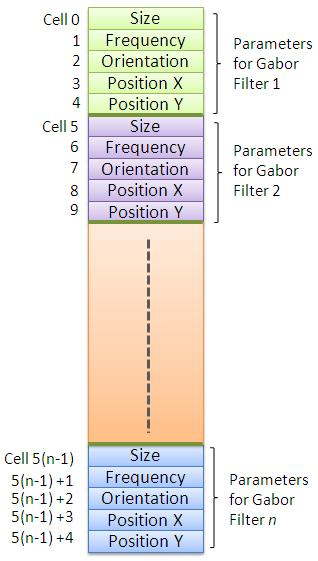
\includegraphics[width = 2in] {Chromosome.JPG}
\caption{A typical chromosome used in the proposed method.}
\label{Fig:Chromosome}
\end{center}
\end{figure}

\subsubsection{The Chromosome}
Each parent per generation encodes the parameters of a set of Gabor
filters in the form of a chromosome. In our implementation, each
Gabor filter is represented by five parameters. If there are $n$
Gabor filters, parameters for all of these filters are encoded into
the chromosome in a serial manner, as shown in Figure
\ref{Fig:Chromosome}. Thus the length of the chromosome is $5n$. The
number of Gabor filters being used per face image determines the
length of the chromosome. As shown in Figure \ref{Fig:Chromosome},
each parameter in the chromosome is encoded as a gene. The
boundaries of these genes defines the regions where the chromosome
undergoes both the crossover and mutation. The genes can be
considered as the primary element of the parent responsible in the
evolution.

\begin{figure}
\begin{center}
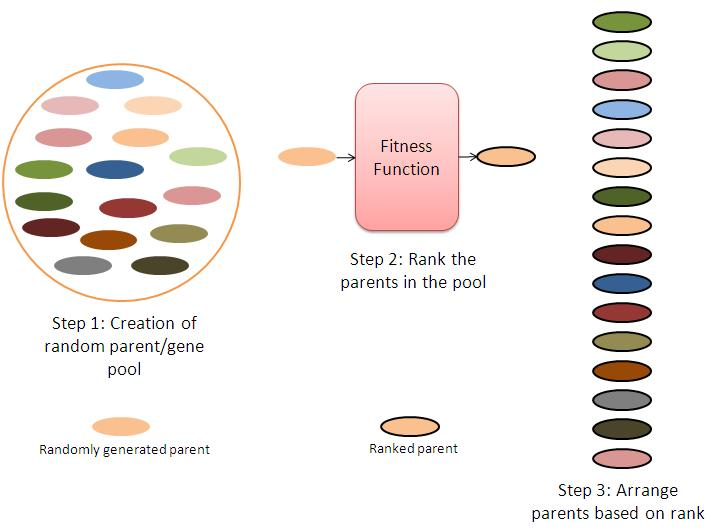
\includegraphics[width = 4in] {Ranking.JPG}
\caption{Stages in the creation of the first generation of parents}
\label{Fig:FirstGen}
\end{center}
\end{figure}

\subsubsection{Creation of the first generation}
Figure \ref{Fig:FirstGen} depicts the first generation of parents,
which are created randomly. Each parent's chromosome is filled
randomly with parameter values where, each parameter value is within
the allowed range for that parameter. Thus, in our experiment, each
parent potentially has the parameters needed for it to perform face
recognition using Gabor filters for feature extraction.

\begin{figure}
\begin{center}
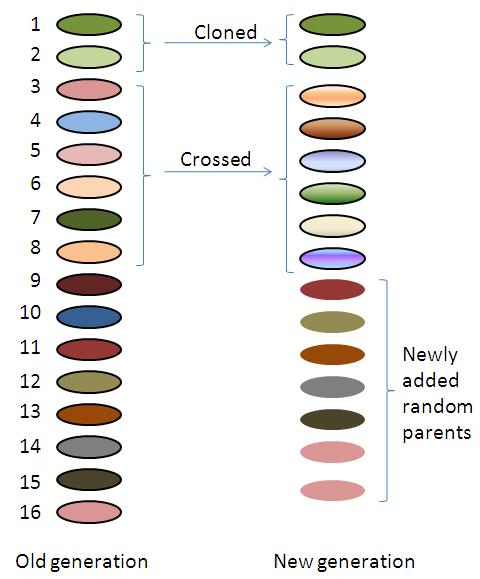
\includegraphics[width = 4in] {Rankorder.JPG}
\caption{Deriving newer parents from the current generation}
\label{Fig:laterGen}
\end{center}
\end{figure}

Once these parents are created, each parent in the gene pool is
evaluated based on its capacity to perform face recognition. To this
end, a fitness function is defined, which takes into account the
ability of each parent to distinguish an individual from all others
based on the most distinguishing features on the individual's face.

This fitness function also takes into account the similarity of the
extracted features, and discourages the selection of features that
are highly correlated with each other. This ensures that the face
images will be searched for multiple distinguishing characteristics.
Subsection \ref{Sec:FF} explains in detail the fitness function used
in our experiments. The parents with the best fitness are ranked
higher, and have the highest probability of being picked for using
genetics the next generation. At the end of the rank ordering
process, the parents are arranged in a descending order, based on
their fitness. This rank ordering determines the probability of each
parent being used to create the subsequent generation. If a parent
has a higher fitness, it will have a higher probability of being
cloned into the next generation, or of otherwise being involved in
reproduction.

\subsubsection{Creation of the newer generations}
The newer generations are created from the older population using
\emph{ clones}, \emph{ mutants}, and \emph{ crossovers} of the fittest
parents. To better search for the optimal parameter set, new random
parents are created every generation. This reduces the likelihood
that the algorithm will get stuck in a local minimum in the search
space.

Figure \ref{Fig:laterGen} shows crossover creates a newer
generation, using the fittest parents from the older generation.

The number of offsprings created from mutation, cloning, and
crossover are determined by parameters of the Genetic algorithm. The
number of clones, mutants, and corssovers are controlled by the
following parameters:

\begin{enumerate}
\item \emph{ Cloning Rate} This parameter controls the number of
parents from the previous generation that will be retained without
undergoing any changes in their genetic structure.
\item\emph{ Crossover Rate} This parameter controls the number of offsprings that will be
born from crossing the parents from the previous generation.
\item \emph{ Mutation Rate} This parameter determines how many of the
crossed offsprings will then be mutated.
\item \emph{ Cloning Distribution Variance} After determining the number of offsprings be to cloned, the
index of the parents for cloning are chosen using a normal
distribution random number generator, with the mean zero and
variance equal to this parameter. Since the parents from the
previous generation have been rank ordered in descending order of
fitness, the zeroth parent will be the top performer (which
coincides with the mean of the random number generator, and has the
highest probability of getting picked).
\item\emph{ Crossover Distribution Variance} This parameter (which is
similar to the Cloning Distribution Variance) is used to choose the
index of the parents who will undergo Crossover.
\end{enumerate}


\begin{figure}
\begin{center}
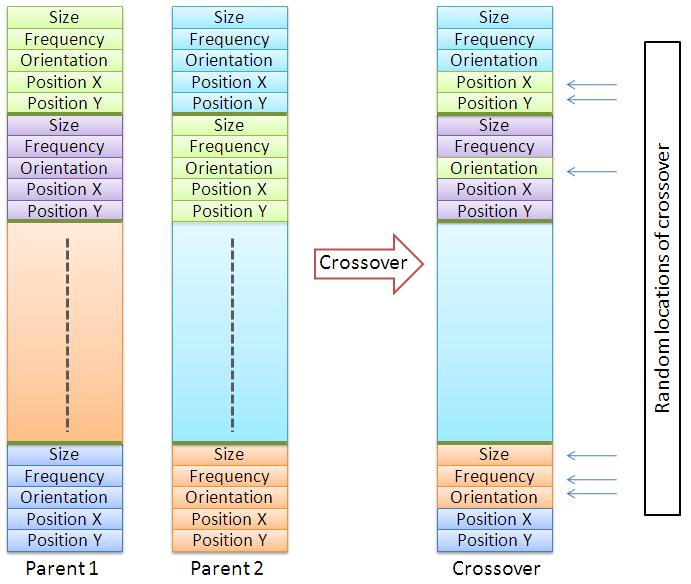
\includegraphics[width = 4in] {Crossover.JPG}
\caption{Typical crossing of two parents to create an offspring}
\label{Fig:CrossOver}
\end{center}
\end{figure}


\subsubsection{\emph{ Crossover}}
As discussed earlier, the parents for crossover are selected by a
random number generator. Between these parents, the points of
crossover are determined by choosing locations of crossover
randomly. As seen in the Figure \ref{Fig:CrossOver}, these locations
are arbitrary gene boundary locations and at these locations the
gene content from the two parents gets mixed. The offspring thus
created now contains parts of the genes coming from the contributing
parents. The motivation for this step is the fact that, as more and
more generations pass, the fittest parents undergoing crossover will
already contain the better sets of parameters, and their crossing
might bring together the better sets of parameter values from both
the parents.

\begin{figure}
\begin{center}
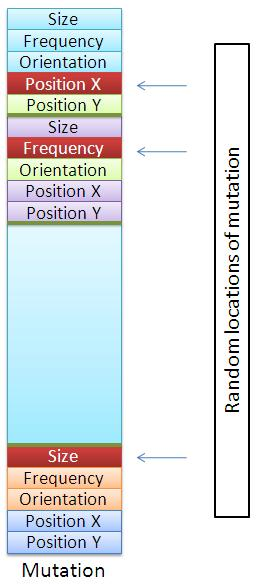
\includegraphics[width = 2in] {Mutation.JPG}
\caption{Mutation of a newly created offspring} \label{Fig:Mutation}
\end{center}
\end{figure}

\subsubsection{\emph{ Mutation}}
In addition to the process of crossover at gene boundaries in the
chromosome, the values of some parameters within the genes might be
changed randomly. This is illustrated in the Figure
\ref{Fig:Mutation}. Such mutations help in exploring the local
parameter space more thoroughly. Mutations can be seen as small
perturbations to the larger search that explores the vast parameter
space, searching for the global minima.

\section{Methodology}
Most feature-based face recognition methods use feature detectors
that are not tailored specifically for face recognition, and they
make no attempt to selectively choose feature detectors based
specifically on their usefulness for face recognition. The method
described in this paper uses Gabor wavelets as feature detectors,
but evaluates the usefulness of each particular feature detector
(and a corresponding $(x,y)$ location) for distinguishing between
the faces within our face database. Given the very large number of
possible Gabor feature detectors and locations, we use a Genetic
Algorithm (GA) to explore the space of possibilities, with a fitness
function that propagates parents with a higher ability to
distinguish between the faces in the database. By selecting the
Gabor feature detectors and locations that are most useful for
distinguishing each person from all of the other people in the
database, we define a unique (i.e. person-specific) feature space
for each person.

\subsection{The FacePix (30) Database}
\label{sec:facepix}

All experiments were conducted with face images from the FacePix
(30) database ~\cite{BLACK2002}. FacePix(30) was compiled to contain
face images with pose and illumination angles annotated in 1 degree
increments. Figure \ref{fig-facepix} shows the apparatus that is
used for capturing the face images. A video camera and a spotlight
are mounted on separate annular rings, which rotate independently
around a subject seated in the center. Angle markings on the rings
are captured simultaneously with the face image in a video sequence,
from which the required frames are extracted.

\begin{figure}[h]
    \centering
        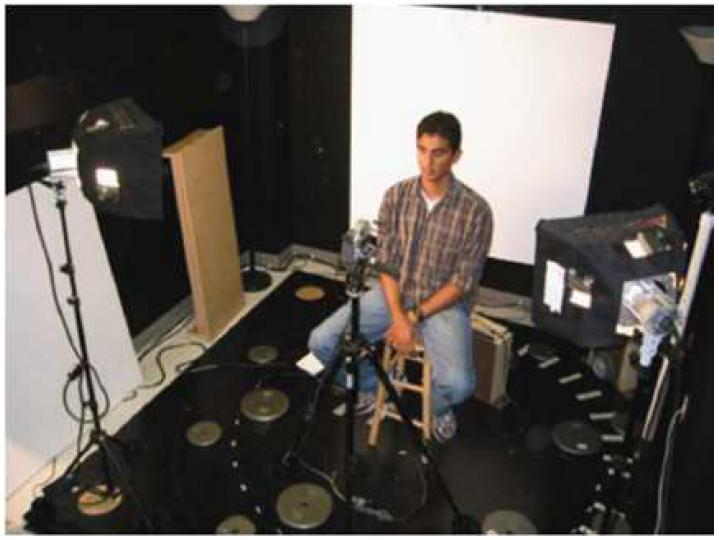
\includegraphics[scale=0.7]{Setup.JPG}
    \caption{The data capture setup for FacePix(30)}
    \label{fig-facepix}
\end{figure}

This database has face images of 30 people across a spectrum of pose
and illumination angles. For each person in the database, there are
three sets of images. (1) The \emph{ pose angle set} contains face
images of each person at pose angles from +90� to �90� (2) The \emph{
no-ambient-light set} contains frontal face images with a spotlight
placed at angles ranging from +90� to -90� with no ambient light,
and (3) The \emph{ ambient-light set} contains frontal face images
with a spot light placed at angles placed at angels from +90� to
-90� in the presence of ambient light. Thus, for each person, there
are three face images available for every angle, over a range of 180
degrees. Figure \ref{fig:facepiximages} provides two examples
extracted from the database, showing pose angles and illumination
angles ranging from -90� to +90� in steps of 10�. For earlier work
using images from this database, please refer ~\cite{Little:2005}.
Work is currently in progress to make this database publicly
available.

\begin{figure}[h]
    \centering
        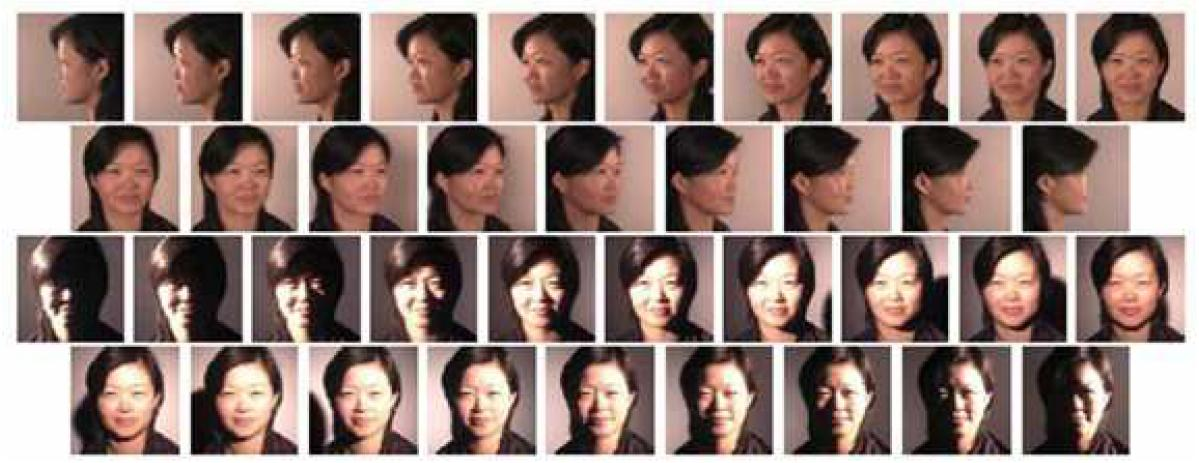
\includegraphics[width = 5.5in]{FacePix.JPG}
    \caption{Sample face images with varying pose and illumination from the FacePix(30) database}
    \label{fig:facepiximages}
\end{figure}

We selected at random two images out of each set of three frontal
(0�) (Figure \ref{facepix}) images for training, and used the
remaining image for testing. The genetic algorithms used the
training images to find a set of Gabor feature detectors that were
able to distinguish each person�s face from all of the other people
in the training set. These feature detectors were then used to
recognize the test images.

\begin{figure}[h]
    \centering
    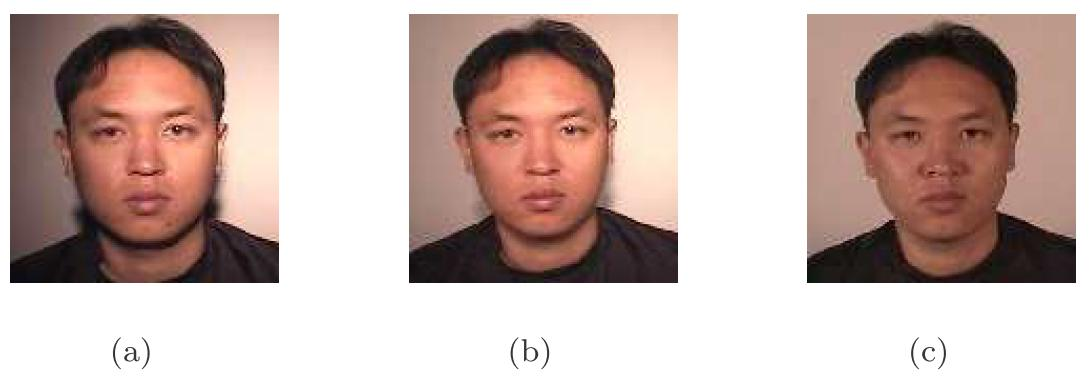
\includegraphics[width=5.5in]{FacePixVariant.JPG}
    \caption{Sample frontal images of one person from the FacePix(30) Database}
    \label{facepix}
\end{figure}

In order to evaluate the performance of our system, we used the same
set of training and testing images with face classification
algorithm based on low-dimensional representation of face images
extracted through Principal Component Analysis
~\cite{sirovich_low-dimensional_1987}. Specifically, the performance
of the implementation of PCA-based face recognition followed by
~\cite{Pent1991} was used in our experiments.

\subsection{The Gabor Features}
Each Gabor feature corresponds to a particular Gabor wavelet (i.e. a
particular special frequency, a particular orientation, and a
particular Gaussian-defined spatial extent) applied to a particular
(x, y) location within a normalized face image. (Given that 125
different Gabor filters were generated, by varying $\omega$,
$\sigma$ and $\theta$ in 5 steps each, and given that each face
image contained $128 \times 128 = 16,384$ pixels, there was a pool
of $125 \times 16384 = 2,048,000$ potential Gabor features to choose
from.) We used an N-dimensional vector to represent each person's
face in the database, where N represents the predetermined number of
Gabor features that the Genetic Algorithm selected from this pool.
Figure \ref{fig:facedots} shows an example face image, marked with 5
locations where Gabor features will be extracted (i.e. N = 5). Given
any normalized face image, real number Gabor features are extracted
at these locations using Equation \ref{Eqn:GaborCoeff}. This process
can be envisioned as a projection of a 16,384-dimensional face image
onto an N dimensional subspace, where each dimension is represented
by a single Gabor feature detector.

\begin{figure}
\begin{center}
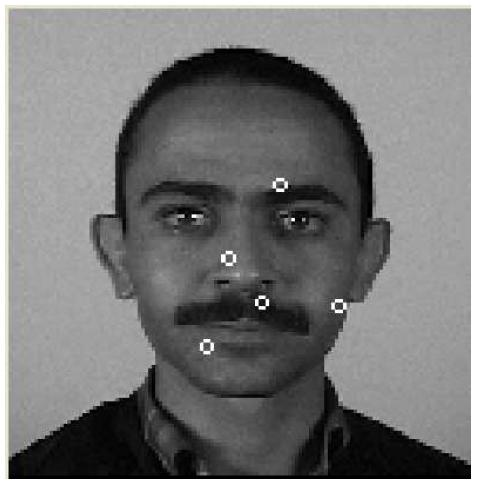
\includegraphics[scale = 0.5] {Result.JPG}
\caption{A face image marked with 5 locations where unique Gabor
features were extracted} \label{fig:facedots}
\end{center}
\end{figure}

Thus, the objective of the proposed methodology is to extract an N
dimensional real-valued person-specific feature vector to
characterize each person in the database. The N (x, y) locations
(and the spatial frequency and spatial extent parameters of the N
Gabor wavelets used at these locations) are chosen by a GA, with a
fitness function that takes into account the ability of each Gabor
feature detector to distinguish one face from all the other faces in
the database.

\subsection{The Genetic Algorithm}
Every GA is controlled in its progress through generations with a
few control parameters such as,
\begin{itemize}
\item the number of generations of evolution ($n_g$)
\item the number of parents per generation ($n_p$)
\item the number of parents cloned per generation ($n_c$)
\item the number of parents generated through cross over ($n_{co}$)
\item the number of mutations in every generation ($n_m$)
\end{itemize}

In our experiments, the GA used the following empirically-chosen GA
parameters: $n_g = 50$, $n_p = 100$, $n_c=6$, $n_{co}=35$ and
$n_m=5$.

\subsubsection{The Fitness Function \label{Sec:FF}}
The fitness function of a genetic algorithm determines the nature of
the search conducted over the parameter space. For face recognition
applications, the fitness function is the capacity of a parent to
classify the individuals accurately. In our proposed method, the
fitness function needs to take both the Gabor features and the
corresponding feature locations into consideration when evaluating
face classification. We define here a fitness function that has two
components to it. One determines the capacity of the parent to
isolate an individual's face image from the others in the database,
and the other evaluates whether the feature is redundant with other
extracted features (i.e. whether a feature detector produces
coefficients that are highly correlated with the coefficients
produced by another feature detector.) Thus the fitness $F$ can be
defined as

\begin{equation}
F = w_{D} D - w_{C} C \label{Eqn:Fitness}
\end{equation}

where $D$ is the distance measure weighted by $w_{D}$, and $C$
represents the correlation measure which measure the similarity
between the coefficients that have been extracted. The correlation
measure $C$ is weighted by the factor $w_{C}$.

If a parent extracts features from a face image that distinguish one
individual from all the others very well (compared to the other
parents within the same generation) then the distance measure $D$
will be the largest for that parent, making its fitness $F$ large.
If the correlation between the extracted features is small, $C$ will
be small, which also makes the fitness $F$ large. Thus, the
correlation measure serves as a \emph{penalty} for extracting the
same feature from the face image multiple times, even though that
particular feature might be the best distinguishing feature on that
face.

The correlation between coefficients was used instead of spatial
separation to counter the problem of similar features being
extracted, because the Gabor filters might not be able to represent
the underlying image characteristic completely. If there are some
large image features on the face (such as beard) that require
multiple Gabor features within a certain spatial locality. Setting a
hard lower limit on this spatial separation might lead to
insufficient representation of that large image feature, in terms of
the Gabor filters.

Consider a parent searching for a unique set of $M$ Gabor filters to
distinguish one individual's face from all other faces. Let this set
of filters be referred to as $S$. Thus, $S = \left\{G_1, G_2,
\cdots, G_M \right\}$ where, $G_m$ represents the $m^{th}$ Gabor
filter.

If the set all individuals in the database is referred to as $I =
\left\{i_1, i_2, \cdots, i_j\right\}$ with $J$ number of
individuals, then for every individual $i$ in $I$ a set $S_i$ has to
be extracted. To achieve this, all the images in the database
depicting individual $i$ are marked as positives, and the ones not
depicting that individual are marked as negatives. Let the set of
positive images be referred to as $P_i$ (with $L$ number of images)
and the set of negatives be referred to as $N$ (with $K$ number of
images). Thus, $S_i = \left\{G_{1i}, G_{2,i}, \cdots, G_{mi}
\right\}$, $P_i = \left\{p_{1i}, p_{2i}, \cdots, p_{li}\right\}$ and
$N_i = \left\{ n_{1i}, n_{2i}, \cdots, n_{ki} \right\}$ are the sets
of Gabor filters, positive images and negatives images set
respectively for the individual $i$.

\begin{itemize}
\item \textbf{ The Distance Measure} $D$ \\
A parent trying to recognize an individual $i$ with a Gabor filter
set $S_i$ can be thought of as a transformation that projects all of
the face images from the image space to a $M$-dimensional space,
where the dimensions are defined by the $M$ Gabor filters in the set
$S_i$. Thus, all of the images in the two sets $P_i$ and $N_i$ can
be considered as points on this $M$-dimensional space. Since the
goal of the genetic algorithm is to find the set $S_i$ which best
distinguishes the individual $i$ from others, in our method we
search for the $M$ dimensional space (defined by a parent) that best
separates the points formed by the sets $P_i$ and $N_i$. Figure
\ref{Fig:Fitness} is an illustration of hypothetical set of face
images projected on a 2 dimensional space defined by a set of 2
Gabor filters $S_i = \left\{ G_0, G_1 \right\}$. As shown in the
figure, the measure $D$ is the minimum of all the Euclidian
distances between every positive and negative points.

Thus, $D$ can be defined as follow:
\begin{equation}
D = \min_{\forall \hspace{0.09in} l,k} \left[\delta_M
\left(\phi_M(p_{li}), \phi_M(n_{ki})\right)\right]
\end{equation}

where, \\
 $\delta_M (A, B) = \sqrt {(a_1 - b_1)^2 + (a_2 - b_2)^2 +
\cdots + (a_m - b_m)^2}$ is the $M$-dimensional Euclidian distance
between $A$ and $B$. $a_x$ and $b_x$ corresponds the $x^{th}$-coordinate of $A$ and $B$ respectively\\
$\phi_M(X)$ is the transformation function that projects image $X$
from the image space to the $M$-dimensional space defined by the set
of Gabor filters.

\begin{figure}
\begin{center}
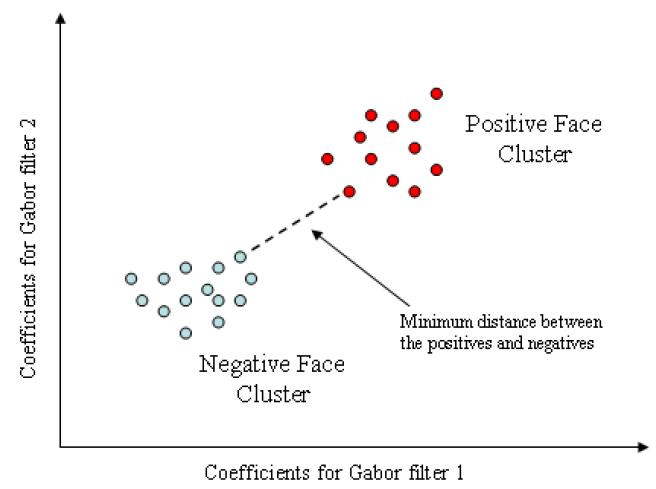
\includegraphics[width = 3in] {Distance.JPG}
\caption{Distance Measure $D$ for the fitness function}
\label{Fig:Fitness}
\end{center}
\end{figure}

\item \textbf{ The Correlation Measure} $C$ \\
In the proposed method, in addition to having every parent selecting
the Gabor filter set $S_i$ that can best distinguish the individual
$i$ from all the others in the database, it is necessary to ensure
that this set of Gabor filters does not include filters that extract
identical image features. If there were no such constraint, the
algorithm might find one very distinguishing image feature on the
face image and, over generations of evolution, all of its Gabor
filters might converge to this one image feature. To avoid this, the
correlation measure $C$ determines the correlation between the image
features extracted at all the locations pointed to by the
chromosome. To test for correlations between the Gabor features at
the different spatial locations, we use the entire set of 125 Gabor
filters to thoroughly characterize the textural context at these
locations.

Assuming that there are $M$ Gabor features that we are looking for
on the face image of individual $i$, let $(x_m, y_m), m = 1, 2,
\dots,M$ be the $M$ points that have been selected genetically in
the chromosome. To find the correlations of the image features
extracted at each of these points, the $N$ Gabor filters $G_i, i =
1, 2, \dots, N$ are used to characterize each of the points. Let the
coefficients of such a characterization be represented by a matrix
$A$. Thus, matrix A is $M \times N$ in dimension, where the rows
correspond to the $M$ locations and $N = 125$ refers to the Gabor
filter coefficients. Thus,

\begin{equation}
A = \left[ \begin{array}{cccc}
g_{(1,1)} & g_{(1,2)} & \ldots & g_{(1,N)}\\
g_{(2,1)} & g_{(2,2)} & \ldots & g_{(2,N)}\\
\vdots  & \vdots  & \vdots & \vdots \\
g_{(m,1)} & g_{(m,2)} & \ldots & g_{(m,N)}
\end{array} \right]
\end{equation}

where, $g_{(m,n)}$ is the coefficient obtained by applying the
$n^{th}$ Gabor filter to the image at the point $(x_m,y_m)$.

The Correlation measure can now be defined in terms of matrix $A$ as
follows

\begin{equation}
C = \log \left(\det \left( diag(B) \right) \right) - \log \left(
\det (B) \right) \label{Eqn:CorrelationMeasure}
\end{equation}

where, $diag (B)$ returns the diagonal matrix corresponding to $B$,
and $B$ is the covariance matrix defined by $B = \frac{1}{N - 1}
(AA^T)$.

Examining the Equation \ref{Eqn:CorrelationMeasure}, it can be seen
that the first log term gets closer to the second log term when the
off diagonal elements of B reduces. The diagonal elements of the
matrix $B$ corresponds to the variance of the $M$ image locations,
whereas the off diagonal elements correspond to the covariance
between pairs if locations. Thus, as the covariance between the
image points decreases, the value of the overall correlation
parameter decreases.

\item \textbf{ Normalization of} $D$ \textbf{ and} $C$ \\
In order to have an equal representation of both the Distance
measure $D$ and the Correlation term $C$ in the fitness function, it
is necessary to normalize the range of values that they can take.
For each generation, before the fitness values are used to rank the
parents, parameters $D$ and $C$ are normalized to range between $0$
and $1$.

\begin{eqnarray}
D_{norm} = \frac{D - D_{Min}}{D_{Max} - D_{Min}} \\
C_{norm} = \frac{C - C_{Min}}{C_{Max} - C_{Min}}
\end{eqnarray}

where, the $Max$ represents the maximum value of $D$ or $C$ in a
single generation across all the parents and $Min$ refers to the
minimum value.

\item \textbf{ Weighting factors} $w_{D}$ \textbf{ and} $w_{C}$ \\
The influence of the two components of the fitness function are
controlled by the weighting factors $w_{D}$ and $w_{C}$. We used the
relation $w_{C} = 1 - w_{D}$ to control the two parameters
simultaneously. With this relationship, a value of $w_{D} \approx 1$
will subdue the effect of the Correlation measure, causing the
genetic algorithm to choose the Gabor filters on the most prominent
image feature alone. On the other hand, $w_{D} \approx 0$ will
subdue the Distance measure, deviating the genetic algorithm from
the main goal of face recognition. Thus an optimal value for the
weight $w_{D}$ has to be estimated empirically, to suit the face
image database in question.

\end{itemize}

\section{Results}
To evaluate the relative importance of the two terms ($D$ and $C$)
in the fitness function, we ran the proposed algorithm on the
training set several times with 5 feature detectors per chromosome,
while changing the weighting factors in the fitness function for
each run, setting $w_D$  to 0, .25, .50, .75, and 1.00, and
computing $w_C = (1-w_D)$. Figure \ref{RES1} shows the recognition
rate achieved in each case.

\begin{figure}
\begin{center}
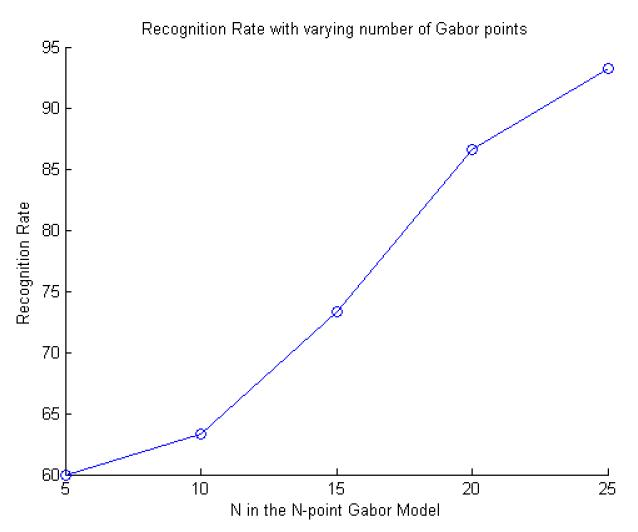
\includegraphics[width = 4in] {Result1FR.JPG}
\caption{The recognition rate versus the number Gabor feature
detectors} \label{RES1}
\end{center}
\end{figure}


We then ran the proposed algorithm on the training set 5 times,
while changing the number of Gabor feature detectors per parent
chromosome for each run to 5, 10, 15, 20, and 25. In all the trials,
$w_D$=0.5. Figure \ref{RES2} shows the recognition rate achieved in
each case.


\begin{figure}
\begin{center}
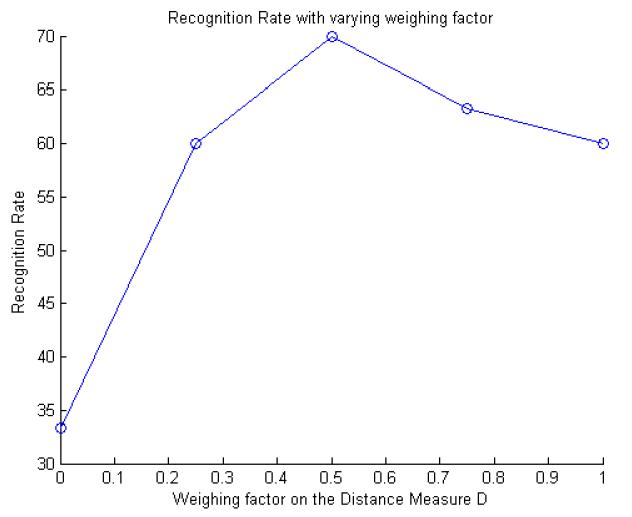
\includegraphics[width = 4in] {Result2FR.JPG}
\caption{Recognition rate with varying $w_D$}\label{RES2}
\end{center}
\end{figure}

\subsection{Discussion of Results}
Figure \ref{RES1} shows that the recognition rate of the proposed
algorithm when trained with 5, 10, 15, 20, and 25 Gabor feature
detectors increases monotonically, as the number of Gabor feature
detectors (N) is increased. This can be attributed to the fact that
increasing the number of Gabor features essentially increases the
number of dimensions for the Gabor feature detector space, allowing
for greater spacing between the positive and the negative clusters.

Figure \ref{RES2} shows that for N = 5 the recognition rate was
optimal when the distance measure D and the correlation measure C
were weighted equally, in computing the fitness function F. The dip
in the recognition rate for $w_D=0.75$ and $w_D=1.0$ indicates the
significance of using the correlation factor C in the fitness
function. The penalty introduced by C ensures that the GA searches
for Gabor features with different textural patterns. If no such
penalty were be imposed, the GA might select Gabor features that are
clustered on one salient facial feature, such as a mole.

The best recognition results for the proposed algorithm (93.3\%)
were obtained with 25 Gabor feature detectors. The best recognition
performance for the PCA algorithm was reached at about 15
components, and flattened out beyond that point, providing a
recognition rate for the same set of faces that was less than
83.3\%. This indicates that, for the face images used in this
experiment (which included substantial illumination variations) the
proposed method performed substantially better than the PCA
algorithm.

\subsection{Person-specific feature extraction}
When the FacePix(30) face database was built, all but one person
were captured without eyeglasses or a hat.  Figures
\ref{fig:result1}(a) and \ref{fig:result1}(b) show the results of
extracting 10 and 20 distinguishing features from that person's face
images. The important things to note about these results are:
\begin{enumerate} \item  At least half of the extracted
Gabor features (8 of the 10) and (10 of the 20) are located on (or
near) the eyeglasses. \item As the number of Gabor features was
increased from 10 to 20, more Gabor features are seen toward the
boundaries of the images. This is due to the fact that the genetic
algorithm chooses Gabor feature locations based on a Gaussian
probability distribution that is centered over the image, and
decreases toward the boundaries of the images.
\end{enumerate}


\begin{figure}[h]
    \centering
    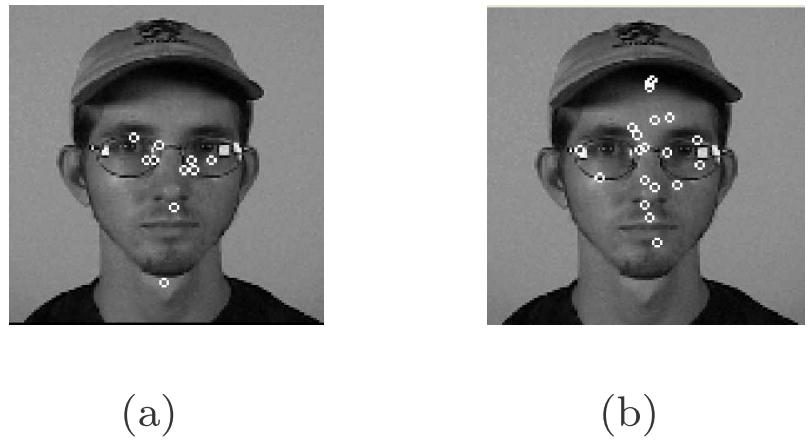
\includegraphics[width=4in]{ResultFR.JPG}
    \caption{10 and 20 person-specific features extracted for a particular individual in the database}
    \label{fig:result1}
\end{figure}

These results suggest that person-specific feature extraction might
be useful for face recognition in small face databases, such as
those typical of a social interaction assistance device for people
who are blind.

\section{Conclusions and Future Work}
As mentioned earlier, the proposed person-specific approach to
evolutionary feature selection in face images is well-suited for
applications such as those that enhance social interaction for
people who are blind, because people do not generally disguise their
appearance in normal social situations, and even when some
significant change occurs (such as a man shaving off his beard) the
system can continue to evolve as it captures new images with each
encounter.

A wearable social interaction assistant prototype has been
implemented using a pair of eyeglasses equipped with a tiny
unobtrusive video camera in the nose bridge ~\cite{Sreekar2005} and
is shown in Section XXXX, Figure XXXX. The analog video output from this
camera is passed through a video digitizer, and the resulting
digital stream is then fed into a portable laptop computer. A video
stream is captured of any person standing in front of the
eyeglasses.  A face detection algorithm, based on Adaboost ~\cite{
violajones01}, is then used to identify the frames of the video
where a face is present, and to localize that face within that
frame. This detected face is then cropped and compared to indexed
faces in a face database.


The performance of the proposed approach for identifying
person-specific features relies, to a large extent, on obtaining
near-frontal views of faces.  To offset this limitation, there is
ongoing work ~\cite{ Balasubramanian2007} to perform
person-independent head pose estimation on the face images obtained
from this platform. It is expected that this will help us select
face images from the video stream with near-frontal views, which
will improve the performance of our algorithm in identifying
person-specific features.

Another factor that limits the performance of our algorithm is
illumination variations in the captured images. Especially
problematic are variations between outdoor-indoor and day-night
settings. (Of course, this limitation is not unique to our
algorithm.) As a strategy to provide additional light unobtrusively
under adverse lighting conditions, we are employing infra-red LED
illuminators in conjunction with an infrared-sensitive camera.

In summary, while there have been many different feature-based
approaches to face recognition over the last two decades of
research, we have proposed a novel methodology based on the
discovery and extraction of person-specific characteristic features
to improve face recognition performance for small face databases.
This approach is aimed at facilitating social interaction in casual
settings. The use of Gabor features, in tandem with a genetic
algorithm to discover characteristic person-specific features has
been inspired by the human visual system and is based on knowledge
that has been developed about the process by which humans recognize
faces.  We believe that more needs to be learnt about human face
recognition, and that as more is learnt, the knowledge can be put to
use to develop more robust face recognition algorithms.


\chapter{SENSING INTERPERSONAL SPACES}
\DoubleSpacing
\setlength{\parindent}{.5in}

In behavioral psychology, influences of interpersonal distances on social interactions between people have been studied for over four decades. The term proxemics, coined by Edward T. Hall, describes influence of interpersonal distances in animal and man \cite{hall_hidden_1990}. The following list describes the American proxemic distances; note that such distances vary with culture and environment.

\begin{enumerate}[1.]
\item Intimate Distance (Close Phase): 0-6 inches
\item Intimate Distance (Far Phase): 6-18 inches
\item Personal Distance (Close Phase): 1.5-2.5 feet
\item Personal Distance (Far Phase): 2.5-4 feet
\item Social Distance (Close Phase): 4-7 feet
\item Social Distance (Far Phase): 7-12 feet
\item Public Distance (Close Phase): 12-25 feet
\item Public Distance (Far Phase): 25 feet or more
\end{enumerate}

Proxemics plays a very important role in interpersonal communication, but people who are blind and visually impaired do not have access to this information. In \cite{ram_people_1998}, Ram and Sharf introduced The People Sensor: an electronic travel aid, for individuals who are blind, designed to help detect and localize people and objects in front of the user. The distance between the user and an obstacle is found using ultrasonic sensors and communicated through the rate of short vibratory pulses, where the rate is inversely proportional to distance. However, the researchers did not do any user testing to determine the usefulness of their technology. Similar to this system, our technology uses the haptic belt described in Chapter 2 for delivering the proxemics information to an individual who is blind or visually impaired.

Tactile rhythms delivered using a vibrotactile belt were used in \cite{erp_waypoint_2005} to convey distance information during waypoint navigation. Time between vibratory pulses was varied using one of two schemes: monotonic (rate is inversely proportional to distance) or three-phase-model (three distinct rhythms mapped to three distances). Distinct tactile rhythms are promising for use with multidimensional tactons \cite{barralon_development_2007} \cite{brown_first_2005}, which are vibratory signals used to communicate abstract messages \cite{brown_first_2005} by changing the dimensions of the signal including frequency, amplitude, location, rhythm, etc. Based on pilot test results, we chose to pursue distinct rhythms over monotonic rhythms as users find it difficult to identify interpersonal distances using monotonic rhythms as the vibratory signal varies smoothly with changes in distance.

From the sensing perspective we resort to the camera that is on the user's glasses and through the use of computer vision technology, face detection, we extract non-verbal cues for social interaction, including the number of people in the user's visual field, where people are located relative to the user, coarse information related to gaze direction (pose estimation algorithms could be used to extract finer estimates of pose), and the approximate distance of the person from the user based on the size of the face image.

\section{Conceptual Framework}
As shown in Figure 1, the output of the face detection process (indicated by a green rectangle on the image) provided by the Social Interaction Assistant is directly coupled with the haptic belt. Every frame in the video sequence captured by the Social Interaction Assistant is divided into 7 regions. After face detection, the region to which the top-left corner of the face detection output belongs is identified (as shown by the star in Figure 3). This region directly corresponds to the tactor on the belt that needs to be activated to indicate the direction of the person with respect to the user. To this end, a control byte is used to communicate between the software and the hardware components of the system. Regions 1 through 7 are coded into 7 bits on the parallel port of a PC. Depending on the location of the face image, the corresponding bit is set to 1. The software also controls the duration of the vibration by using timers. The duration of a vibration indicates the distance between the user and the person in his or her visual field. The longer the vibration, the closer the people are, which is estimated by the face image size determined during the face detection process.

An overall perspective of the system and its process flow is given below. When a user encounters a person in his or her field of view, the face is detected and recognized (if the person is not in the face database, the user can add it). The delivery of information comprises two steps: Firstly, the identity of the person is audibly communicated to the user (we are currently investigating the use of tactons \cite{brewster_tactons:_2004} to convey identities through touch, but this is part of future work). Secondly, the location of the person is conveyed through a vibrotactile cue in the haptic belt, where the location of the vibration indicates the direction of the person and the duration of vibration indicates the distance between the person and the user. Based on user preference, this information can be repeatedly conveyed with every captured frame, or just when the direction or distance of the person has changed. The presence of multiple people in the visual field is not problematic as long as faces are not occluded and can be detected and recognized by the Social Interaction Assistant. We are currently investigating how to effectively and efficiently communicate non-verbal communication cues when the user is interacting with more than one person.

**********************************
In this chapter we introduce the sensing and the delivery end of the system that can deliver proxemics information to an individual who is blind or visually impaired. From the sensing end, we describe a face detection methodology that is capable of identifying exact boundaries of the face region through which we model the distance of the interaction partner from the person who is using the device. From the delivery end, we describe user tests that were conducted to determine the use of tactons for conveying direction and distance information.
**********************************



\section{Accurate Face Detection}\label{Introduction} \vspace{-0.2in} Face
detection has become an important first step towards solving
plethora of other computer vision problems like face recognition,
face tracking, pose estimation, intent monitoring and other face
related processing. Over the years many researchers have come up
with algorithms, that have over time, become very effective in
detecting faces in complex backgrounds. Currently, the most popular
face detection algorithm is the Viola-Jones \cite{viola_robust_2004}
face detection algorithm whose popularity is boosted of by its
availability in the open source computer vision library, OpenCV.
Other popular face detection algorithms are identified in
\cite{hjelm�s_face_2001} and \cite{ming-hsuan_yang_detecting_2002}.

Most face detection algorithms learn faces by modeling the intensity
distributions in upright face images. These algorithms tend to
respond to face-like intensity distributions in image regions that
do not depict any face as they are not contextually aware of the
presence or absence of a human face. These spurious responses make
the results unsuitable for further processing that requires accurate
face images as inputs, such as the ones mentioned above. Figure
\ref{Fig:ExampleFalseDetect} shows an example where a face detection
algorithm detects two faces - one true and the other false.

\begin{figure}[h]
\centering
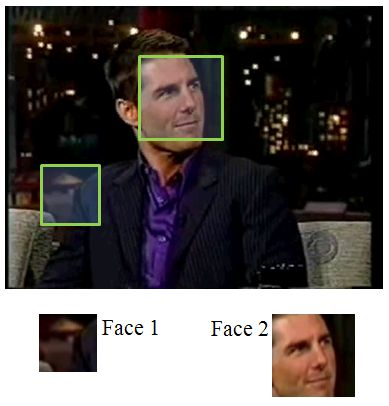
\includegraphics[width=3in]{Figure1.jpg}
\caption{An example false face detection.} \label{Fig:ExampleFalseDetect}
\end{figure}

The problem of false face detection has motivated some researchers
to develop heuristic approaches aimed for validating the face
detection results. Most of these heuristics integrate primitive
context into the problem by searching for skin tone in the output
subimages. However, this simple approach often fails to distinguish
faces from non-faces, because face detectors often fail to center
the cropping box precisely around the detected face. This produces a
significant patch of skin colored pixels, but only a partial face.
This centering problem can be dealt with by extracting the skin
colored regions and comparing their shape to an ellipse. While such
heuristics, are simple, and somewhat effective, their validation is
not reliable enough to meet the needs of higher level face
processing tasks. Further, they do not provide a confidence metric
for their validation.


\begin{figure}[h]
\centering
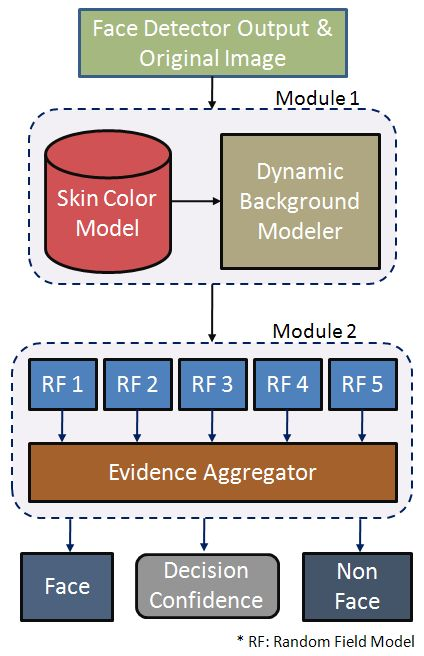
\includegraphics[width=3.5in]{Figure2.jpg}
\caption{Block diagram.}
\label{Fig:BlockDiagram}
\end{figure}

This paper treats the problem of face detection validation in a
systematic manner, and proposes a learning framework that
incorporates both contextual and structural knowledge of human
faces. A face validation filter is designed by combining two
statistical modelers, 1) a human skin-tone detector with a dynamic
background modeler (Module $1$), and 2) an evidence-aggregating
human face silhouette random field modeler (Module $2$), which
provides a confidence metric on its validation task. The block
diagram in Figure \ref{Fig:BlockDiagram} shows the functional flow
of data through the two modules in the proposed framework. The
details of the statistical models and their learning will be
presented later in the paper, which is organized as follows. Section
2 reviews some of the earlier research. Section 3 introduces the
proposed framework, with details on the learning process. Section 4
discusses the experiments carried out to test the proposed
framework. Section 5 presents the results while Section 6 discusses
them. Section 7 concludes the paper and discusses future work.

%-------------------------------------------------------------------------
\section{Related Work}\label{RelatedWork} \vspace{-0.2in} As
mentioned earlier, the problem of face detection validation has not
been treated methodically before, though the problem has been
handled by many as an integral component of face detection
algorithms. All the past work in this area can be broadly
characterized into two groups: a) Low level image feature models
mostly based on skin color such as \cite{a_hadid_hybrid_2006},
\cite{naseem_robust_2005} and \cite{m_wimmer_person_2006}, and b)
High level facial feature models such as \cite{hmid_fuzzy_2006},
\cite{tariq_face_2004} and \cite{yan-wen_wu_face_2008}.

The low level skin color based approaches try to reduce
computational complexity by first identifying skin color in images
so that search can be reduced. Most of the times, simple geometrical
properties of the retained skin regions are used to determine if the
region is a face. Such simplification of faces into trivial
geometrical structures results in false detections. The facial
feature based methods achieve face detection by individually
identifying the integral components of a face image such as eyes,
nose, etc. Though these schemes could be robust, the associated
computational load is high. Interested readers could find more
related references in \cite{ming-hsuan_yang_detecting_2002} and
\cite{hjelm�s_face_2001}. The framework proposed in this paper uses
statistically learnt knowledge about human faces to overcome
computational complexity thereby augmenting face validation to
existing face detection algorithms seamlessly.

%-------------------------------------------------------------------------
\section{Proposed Framework}\label{ProposedFramework}
\vspace{-0.2in} As shown in Figure \ref{Fig:BlockDiagram}, the
framework essentially has two statistically learnt models, Module
$1$ and Module $2$, that are cascaded to form the face detection
validation filter. The output from a face detector is sent to Module
$1$, which distinguishes the skin pixels in the face region from the
background pixels, thereby constucting a skin region mask. This skin
region mask then becomes the input to Module $2$, which is
essentially an aggregate of random field models learnt from manually
labeled ({\emph true}) face detection outputs. The results of each
random field model within the aggregate are then combined, using
rules of Dempster-Shafer Theory of Evidence
\cite{sentz_combination_2002}. This {\emph combining of evidence}
provides a metric for the belief (i.e. confidence) of the system in
its final validation. The two modules are detailed in the following
subsections.
%-------------------------------------------------------------------------
\subsection{Module $1$: Human Skin Tone Detector with Dynamic
Background Modeler}\label{Module1} \vspace{-0.2in} Most of the skin
tone detectors used for human skin color classification use prior
knowledge, which is provided in the form of a parametric or
non-parametric model of skin samples that are extracted from images
- either manually, or through a semiautomated process. In this paper
we employ such an a priori model, in combination with a dynamic
background modeler, so that the skin vs. non-skin boundary is
accurately determined. Accurate skin region extraction is essential
for Module $2$, as it validates images based on their structural
properties. The two functional components of Module $1$ are:

\subsubsection{{\em a-priori} Bi-modal Gaussian Mixture Model
for Human Skin Classification}\label{Bi-ModGaussian}
\vspace{-0.1in}A normalized RGB color space has been a popular
choice among researchers for parametric modeling of human skin
color. The normalized RGB (typically represented as nRGB) of a pixel
$X$ with $X_r$, $X_g$, $X_b$ as its red, green and blue components
respectively, is defined as:
\begin{equation}
X_{i|i \in \{r,g,b\}}^{nRGB} =
\frac{X_i}{\left(\sum\limits_{\forall_{i|i\in\{r,g,b\}}}X_i\right)}
\end{equation}
Normalized RGB space has the advantage that only two of the three
components, nR, nG or nB, is required at any one time to describe
the color. The third component can be derived from the other two as:
\begin{equation}
X_{i|i \in \{nR,nG,nB\}}^{nRGB} =  1 -\left(
\sum_{\forall_{k|(k\in\{nR,nG,nB\}, k \ne i)}}X_k \right)
\end{equation}

\vspace*{-0.3in}

\begin{figure}[h]
\centering
\includegraphics[width=3in]{Figure3.jpg}
\caption{Skin pixels in nRGB space.} \label{Fig:nRGBProject}
\end{figure}

\vspace{0.1in} In our experiments, we found that skin pixels form a
tight cluster when projected on nG and nB space as shown in the
Figure \ref{Fig:nRGBProject}. The study was based on a skin pixel
database, consisting of nearly $150,000$ samples, built by randomly
sampling skin regions from $1040$ face images collected on the web
as well as from FERET face database \cite{phillips_feret_1997}.
Further analysis also showed that the cluster formed on the 2D nG-nB
space had two prominent density peaks which motivated the modeling
of skin pixels with a Bi-modal Gaussian mixture model learnt using
Expectation Maximization (EM) with a $k$-means initialization
algorithm \cite{bilmes_gentle_1998}. The Bi-modal Gaussian mixture
model is represented as.
\begin{eqnarray}
f^{skin}_{X|X=[nG,nB]}(x) & = & w_1 f_{Y_1}(x;\Theta_1=[\mu_1,\Sigma_1]) +  \nonumber  \\
       &  & w_2 f_{Y_2}(x;\Theta_2=[\mu_2,\Sigma_2])
\end{eqnarray}

\subsubsection{Dynamically Learnt Multi-modal Gaussian Model for
Background Pixel Classification}\label{DynamicModel} \vspace{-0.1in}
As mentioned earlier, classification of regions into face or
non-face requires accurate skin vs. non-skin classification. In
order to achieve this, we learn the background color surrounding
each face detector output dynamically. To this end we extract an
extra region of the original image around the face detector's
output, as shown in Figure \ref{Fig:Extraregion}. Since the size of
the face detector output varies from image to image, it is necessary
to normalize the size. This is done by downsampling the size of the
original image to produce a face detector output region containing
$90$x$90$ pixels. The extra region pixels surrounding the face are
then extracted from the $100$x$100$ region around this $90$x$90$
normalized face region.

\begin{figure}[h]
\centering
\includegraphics[width=2.5in]{Figure4.jpg}
\caption{Extra region for background modeling.} \label{Fig:Extraregion}
\end{figure}

Once the outer pixels are extracted, a Multi-modal Gaussian Mixture
is trained using EM with $k$-means initialization, similar to the
earlier case with skin pixel model. The resultant model can be
represented as.
\begin{equation}
f^{non-skin}_{X|X=[R,G,B]}(x) =
\sum\limits_{i=1}^{m}w(i)f_{Y_i}\left(x;\Theta_i=[\mu_i,\Sigma_i]\right)
\end{equation}
where, $m$ is the number of mixtures in the model. We found
empirically that a value of $m=2$ or $m=3$ modeled the backgrounds
with sufficient accuracy.

\subsubsection{Skin and Background Classification using the learnt
Multi-modal Gaussian Models}\label{SkinnBackground} \vspace{-0.1in}
The skin and non-skin models, $f^{skin}_{X|X=[nG,nB]}(x)$ and
$f^{non-skin}_{X|X=[R,G,B]}(x)$ respectively, are used for
classifying every pixel in the scaled face image obtained as
explained in the Section \ref{DynamicModel}. Example skin-masks are
shown in Figure \ref{Fig:Skinmasks}. This example shows two sets of
images - one corresponding to a {\emph true} face detection result,
and another {\emph false} face detection result.

\begin{figure}[h]
\centering
\includegraphics[width=4in]{Figure5.jpg}
\caption{Example of {\em true} and {\em false} face detection.} \label{Fig:Skinmasks}
\end{figure}

The structural analysis through Random Field models explained in the
next section will describe the design concepts that will help
distinguish between {\emph true} and {\emph false} face detections shown
in Figure \ref{Fig:Skinmasks}.
%-------------------------------------------------------------------------
\subsection{Module $2$: Evidence-Aggregating Human Face Silhouette
Random Field Modeler}\label{Module2} \vspace{-0.2in}
 In order to validate the skin region
extracted as explained in Section \ref{Module1}, we build
statistical models from examples of faces. We developed statistical
learners inspired by Markov Random Fields (MRF) to capture the
variations possible in {\emph true} skin masks (face silhouette). The
following subsections describes MRF models and the variant we
created for our experiments.

\subsubsection{Random Field (RF) Models}\label{MRF} \vspace{-0.1in}
In this work, we used a minor variant of MRFs to learn the structure
of a {\emph true} face skin mask. MRFs encompass a class of
probabilistic image analysis techniques that rely on modeling the
intensity variations and interactions among the image pixels. MRFs
have been widely used in low level image processing including, image
reconstruction, texture classification and image segmentation
\cite{perez_markov_1998}.

In an MRF, the sites in a set, $\mathcal S$, are related to one
another via a neighborhood system, which is defined as ${\mathcal
N}=\{{\mathcal N}_i, i \in \mathcal S\}$, where ${\mathcal N}_i$ is
the set of sites neighboring $i$, $i \notin {\mathcal N}_i$ and $i
\in {\mathcal N}_j \Longleftrightarrow j \in {\mathcal N}_i$.

A random field X said to be an MRF on $\mathcal S$ with respect to a
neighborhood system $\mathcal N$, if and only if,
\begin{eqnarray}&& P({\mathbf x})>0, \forall \mathbf x \in \mathcal X  \\ && P(x_i\vert x_{{\mathcal S}-\{i\}})=P(x_i\vert x_{{\mathcal N}_i}) \label{Eqn:5} \end{eqnarray}
where, $P(x_i\vert x_{{\mathcal S}-\{i\}})$ represents a Local
Conditional Probability Density function defined over the
neighborhood $\mathcal N$. The variant of MRF that we created for
our experiments relaxed the constraints imposed by MRFs on $\mathcal
N$. Typically, MRFs requires that sites in set $\mathcal S$ be
contiguous neighbors. The relaxation in our case allows for distant
sites to be grouped into the same model.

We empirically found out that modeling the skin-region validation
problem into one single RF gave poor results. We devised $5$ unique
RF models with an Dempster-Shafer Evidence aggregating framework
that could not only validate the face detection outputs, but also
provide a metric of confidence. Thus, Equation \ref{Eqn:5} could be
alternatively seen as a set $P({\mathbf x}) = \{P^1({\mathbf x}),
\ldots, P^5({\mathbf x})\}$, each having their own neighborhood
system $\mathcal N^k = \{\mathcal N^1, \mathcal N^2, \ldots,
\mathcal N^5\}$, such that
\begin{equation}
P^k(x_i\vert x_{{\mathcal S}-\{i\}})=P(x_i\vert x_{{\mathcal
N^k_i}})
\end{equation}

\subsubsection{Pre-processing}\label{Preprocessing} \vspace{-0.1in} As described earlier,
each face detector output is normalized and expanded to produce a
$100$x$100$ pixel image, from which a binary skin mask is generated.
A morphological opening and closing operation is then performed on
the skin mask (to eliminate isolated skin pixels), and the mask is
then partitioned into one hundred $10$x$10$ blocks, as shown in
Figure \ref{Fig:RowColumnBlocks}. The number of mask pixels (which
represent skin pixels) are counted in each block, and a $10$x$10$
matrix is constructed, where each element of this matrix could
contain a number between 0 and 100. This $10$x$10$ matrix is then
used as the basis for determining whether the face detector output
is indeed a face.

\begin{figure}[h]
\centering
\includegraphics[width=4in]{Figure6.jpg} \caption{Pre-processing.}
\label{Fig:RowColumnBlocks}
\end{figure}

\subsubsection{The Neighborhood System}\label{Neighborhood} \vspace{-0.1in} The determination of whether the
face detector output is actually a face is based on heuristics that
are derived from anthropological human face models
\cite{vezjak_anthropological_1994} and through our own statistical
analysis. These include:
\begin{enumerate}
\item Human faces are horizontally symmetrical (i.e. along any row of blocks $R_i$)
about a  central vertical line joining the nose bridge, the tip of
the nose and the chin cleft, as shown in Figure
\ref{Fig:RowColumnBlocks}.  In particular, our analysis of a large
set of frontal face images showed that the counts of skin pixels in
the 10 blocks that form each row in Figure \ref{Fig:RowColumnBlocks}
were roughly symmetrical across this central line.

\item The variations along the verticals ($C_i$'s) are negligible enough
that in building a Local Conditional Probability Density function,
each $R_i$ can be considered independent of the other. That is, for
example, modeling variations of $C_0$ w.r.t $C_1$ on $R_1$ is
similar to modeling variations of $C_0$ w.r.t $C_1$ on any other
$R_{i|i\ne1}$. Thus, analysis of Local Conditional Probability could
be restricted to single $R_i$ at a time, as shown in Figure
\ref{Fig:Neighborhood}.
\end{enumerate}

\begin{figure}[h]
\centering
\includegraphics[width=4in]{Figure7.jpg} \caption{Neighborhood System.}
\label{Fig:Neighborhood}
\end{figure}

The different neighborhood systems $\mathcal N^k$, used in the RF
models, $P^k(x\vert x_{\mathcal N^k})$, can be defined as (Refer
Figure \ref{Fig:Neighborhood}):
\begin{equation}
\mathcal N^k = \left\{C_{j | j \in \{|k|, 0^-, 0^+\}}\right\}
\end{equation}

\subsubsection{Local Conditional Probability Density (LCPD)}\label{LCPD} \vspace{-0.1in} To model the
variations on the skin-region mask, we choose to build 2D histogram
for each of the $5$ RF over their unique neighborhood system. The
design of the dimensions were such that they captured the various
structural properties of {\emph true} skin masks. The two dimensions
(represented in a histogram pool ${\mathbf H}^k$) with individual
element of the pool, ${\mathbf z}$, can be defined as:
\begin{itemize}
\item $\mathbf{H}^{k|k=\{1,2,3,4\}} = \left\{ \mathbf{z}\right\}$, where,
\begin{equation}\mathbf{z} = [x_{C_{0^{\pm}}}, \delta(x_{C_{0^{\pm}}},
x_{C_{\pm k}})] , \forall R_{j} \label{Eqn:9}
\end{equation}

\item$\mathbf{H}^{k=5} = \left\{
\mathbf{z}\right\}$, where,
\begin{equation}
\mathbf{z} = [\mu(x_{C_{0^+}},x_{C_{0^-}}), \mu(x_{C_{-4}},
x_{C_{+4}})] , \forall R_{j} \label{Eqn:10}
\end{equation}
\end{itemize}

where, $x_{C_k}$ is the count of skin pixels in the block $C_k$. The
two functions $\delta(.,.)$ and $\mu(.,.)$ are defined as
\begin{eqnarray}
\delta(x_{C_{0^{\pm}}}, x_{C_{\pm i}}) & = & \left\{
\begin{array}{l l}
x_{C_{0^+}} - x_{C_{+i}}, & i>0 \\
x_{C_{-i}} - x_{C_{0^-}}, & i<0 \\
\end{array}
\right. \\
\mu(a,b) & = & \frac{a+b}{2}
\end{eqnarray}
In order to estimate the LCPD on these $5$ histogram pools, we use
Parzen Window Density Estimation (PWDE) technique, similar to
\cite{paget_texture_1997}, with a 2D Gaussian window. Thus, each of
LCPD can now be defined as
\begin{equation}
\begin{array}{l}
 \hspace*{-0.15in}P^k(\mathbf z) = \frac{1}{(2\pi)^{\frac{d}{2}} n h_{opt}^d} \sum\limits_{j=1}^n
 \exp \\     \\
\hspace{1in} \left[-\frac{1}{2 h^2_{opt}} \left(\mathbf{z} - \mathbf
{H}^k_j\right)^T \Sigma^{-1} \left( \mathbf{z} - \mathbf
{H}^k_j\right) \right]    \nonumber
\end{array}
\end{equation}

where, $n$ is the number of samples in the histogram pool
$\mathbf{H}^k$, $d$ is number of dimensions (in our case $2$),
$\Sigma$ and $h_{opt}$ are the covariance matrix over $\mathbf{H}^k$
and the optimal window width, respectively, defined as:
\begin{eqnarray}
\Sigma = \left[\begin{array}{cc} \sigma_{1} & 0 \\ 0 &
\sigma_{2}\end{array} \right], & h_{opt} =
\frac{\sigma_{1}+\sigma_{2}}{2} \left\{\frac{4}{n(2d+1)}
\right\}^{1/(d+4)}          \nonumber
\end{eqnarray}
Figure \ref{Fig:LCPDs} shows the $5$ LCPDs learnt over a set of
$390$ training frontal face images.

\begin{figure}[h]
\centering
\includegraphics[width=4in]{Figure8.jpg}
\caption{Frontal face Local Conditional Probability Density (LCPD) models.} \label{Fig:LCPDs}
\end{figure}


\subsubsection{Human Face Pose}\label{HumanFacePose} \vspace{-0.1in} During our studies we discovered that
the structure of the skin-region varies based on the pose of
detected face as shown in Figure \ref{Fig:PoseMasks}. Combining face
examples from different pose into one set of RFs seemed to dilute
the LCPDs and hence the discriminating capability. This motivated us
to design three different sets of RFs, one for each pose. This was
accomplished by grouping {\emph true} face detections into three
piles, Turned right ($r$), Facing front ($f$), and, Turned Left
($l$).

\begin{figure}[h]
\centering
\includegraphics[width=4in]{Figure9.jpg}
\caption{Skin-region masks.}
\label{Fig:PoseMasks}
\end{figure}

Thus, the final set of LCPDs could be described by the super set.
\begin{equation}
P(\mathbf z) = \left\{P^{k|k=\{1,\ldots,5\}}_{m|m=\{r,f,l\}}(\mathbf
z) \right\}
\end{equation}

\subsection{Combining Evidence}\label{CombiningEvidence}
\vspace{-0.2in} Given any test face detection output, $\mathbf{z}$
is extracted (as described in Equation \ref{Eqn:9} and \ref{Eqn:10})
and projected on the LCPD set $P(\mathbf z)$ to get a set of
likelihoods $l_m^k$. As in the case of any likelihood analysis, we
combined the joint likelihood of multiple projections using
log-likelihood function, $L_m^k = \ln \left(l_m^k\right)$, such
that,
\begin{equation}
\prod\limits_{\forall {\mathbf z} \in {\mathbf H}^k_m}\ln
\left(l_m^k(\mathbf z)\right) =  \sum\limits_{\forall {\mathbf z}
\in {\mathbf H}^k_m}L_m^k(\mathbf z)
\end{equation}
Given these log-likelihood values, one can set hard thresholds on
each one of them to validate a face subimage discretely as {\emph
true} or {\emph false}. We incorporated a piece-wise linear decision
model (soft threshold) instead of a hard threshold on the acceptance
of a face subimage. This is illustrated in the Figure
\ref{Fig:Thresholds}. Each LCPD $P^k(\mathbf z)$ was provided with
an upper and lower threshold of acceptance and rejection
respectively. The upper and lower bounds were obtained by observing
$P^k(\mathbf z)$ for the three face poses $P^k_{r,f,l}(\mathbf z)$.
Thus, any log-likelihood values lesser than the lower threshold
($L_L$) would result in a decision against the test input
(Probability $0$), while any log-likelihood value greater that the
upper threshold ($L_U$) would be a certain accept (probability $1$).
Anything in between would be assigned a probability of acceptance.
\begin{figure}[h]
\centering
\hspace{-0.3in}\includegraphics[width=2.5in]{Figure10.jpg}
\caption{Soft threshold.}
\label{Fig:Thresholds}
\end{figure}
In order to combine the decisions from the five LCPD $P^k(\mathbf
Z)$, we resort to Dempster-Shafer Theory of Evidence.

\subsubsection{Dempster-Shafer Theory of Evidence (DST)}\label{DST}
\vspace{-0.1in} The Dempster-Shafer theory is a mathematical theory
of evidence \cite{sentz_combination_2002} which is a generalization
of probability theory with probabilities assigned to sets rather
than single entities.

If $X$ is an universal set with power set, $\mathbf{P}(X)$ (Power
set is the set of all possible sub-sets of $X$, including the empty
set $\emptyset$), then the theory of evidence assigns a belief mass
to each subset of the power set through a function called the basic
belief assignment (BBA), $m:\mathbf{P}(X) \rightarrow [0,1]$, when
it complies with the two axioms. a) $m(\emptyset) = 0 $ and b)
$\sum\limits_{\mathbf{A} \in \mathbf{P}(X)} m(\mathbf{A})= 1$. The
mass, $m(A)$, of a given member of the power set expresses the
proportion of all relevant and available evidence that supports the
claim that the actual state belongs to $A$ and to no particular
subset of $A$. In our case, $m(A)$ correlates to the probability
assigned by each of  LCPDs towards the subimage being a face or not.

The true use of DST in our application becomes clear with the {\emph
rules of combining evidences} which was proposed as an immediate
extension of DST. According to the rule, the combined mass
(evidence) of any two expert's opinions, $m_1$ and $m_2$, can be
represented as:
\begin{equation}
m_{1,2}(A) = \frac{1}{1-K}\sum\limits_{B\cap C = A, A \ne
\emptyset}m_1(B) m_2(C) \label{Eqn:16}
\end{equation}
where,
\begin{equation}
K = \sum\limits_{B \cup C = \emptyset}m_1(B) m_2(C) \label{Eqn:17}
\end{equation}is a measure of the conflict in the experts opinions. The
normalization factor, $(1-K)$, has the effect of completely ignoring
conflict and attributing any mass associated with conflict to a null
set.

The $5$ LCPDs, $P^k(\mathbf z)$, were considered as experts towards
voting on the test input as a face or non-face. In order to use
these mapped values in Equation \ref{Eqn:16} - \ref{Eqn:17}, we
normalized evidences generated by the experts to map between
$[0,1]$, and any conflict of opinions were added into the conflict
factor, $K$. For the sake of clarity, we show an example of
combining two expert opinions in Figure \ref{Fig:DST}. The same idea
could be extended to multiple experts.

\begin{figure}[h]
\centering
\includegraphics[width=3.5in]{Figure11.jpg}
\caption{An example of combining
evidence from two experts under Dempster-Shafer Theory.}
\label{Fig:DST}
\end{figure}

\subsection{Coarse Pose estimation}\label{CoarsePoseEstimation}
\vspace{-0.2in} Since the RF models were biased with pose
information, we also investigated the possibility of determining the
pose of the face based on the evidences obtained from the LCPDs. We
noticed that the LCPDs $P^3(\mathbf z)$, $P^4(\mathbf z)$ and
$P^5(\mathbf z)$ were capable of not only discriminating faces from
non-faces, but were also capable of voting towards one of $3$ pose
classes, Looking right, Frontal, and Looking Left along with a
confidence metric. Due to space constraints, the procedure is not
explained in detail, but it is similar to what was followed for face
versus non-face discrimination as explained in Section
\ref{CombiningEvidence}.

%-------------------------------------------------------------------------
\section{Experiments}\label{Experiments} \vspace{-0.2in} In all our
experiments, Viola-Jones face detection algorithm
\cite{viola_robust_2004} was used for extracting face subimages. The
proposed face validation filter was tested on two face image data
sets, 1. {\emph The FERET Color Face Database}, and 2. {\emph An
in-house face image database} created from interview videos of
famous personalities.

In order to prepare the data for processing, face detection was
performed on all the images in both the data sets. The number of
face detections do not directly correlate to the number of unique
face images as there are plenty of false detections. We manually
identified each and every face detection to be {\emph true} or {\emph
false} so that ground truth could be established. The details of
this manual labeling is shown below:
\begin{enumerate}
\item {\em FERET}
\begin{itemize}
\item Number of actual face images: $14,051$
\item Number of faces detected using Viola-Jones algorithm: $6,208$
\item Number of {\emph true} detections: $4,420$
\item Number of {\emph false} detections: $1,788$ ($28.8$\%)
\end{itemize}
\item {In-house database}
\begin{itemize}
\item Number of actual face images: $2,597$
\item Number of faces detected using Viola-Jones algorithm: $2,324$
\item Number of {\emph true} detections: $2,074$
\item Number of {\emph false} detections: $250$ ($10.7$ \%)
\end{itemize}
\end{enumerate}

 %-------------------------------------------------------------------------
\section{Results} \label{Sec:Results} \vspace{-0.2in}
 In order to compare the
 performance of the proposed face validation filter, we defined four parameters:
 \begin{enumerate}
 \item Number of false detections (NFD)
 \begin{equation}
\mbox{NFD} = \mbox{Count of false detections} \nonumber
 \end{equation}
 \item False detection rate (FDR): \begin{equation}
 \mbox{FDR} = \frac{\mbox{\# of false detections}}{\mbox{Total \# of face
 detections}} \mbox{x} 100 \nonumber
 \end{equation}
 \item Precision (P)
 \begin{equation}
 \mbox{P} = \frac{\mbox{\# of true detections}}{\mbox{\# of true detections} + \mbox{\# of false
 detections}} \nonumber
 \end{equation}
 \item Capacity (C)
 \begin{equation}
 \mbox{C} = \left(\frac{\mbox{\# of true detections}}{\mbox{\# of actual faces in database}}\right) -
 \mbox{FDR} \nonumber
 \end{equation}
 \end{enumerate}



\begin{table}[h]
\caption{Face detection validation results on FERET database.} \label{Tab:FERET}
\centering
 \begin{tabular}{|c||c|c|}
   \hline
   % after \\: \hline or \cline{col1-col2} \cline{col3-col4} ...
    & Before Validation & After Validation \\
    \hline
    \hline
    NFD  &  $1,788$ & $208$ \\
   FDR & $28.8$ \% & $3.35$ \% \\
   P & $0.7120$ & $0.9551$ \\
   C & $0.026$ & $0.281$ \\
 \hline
\end{tabular}
\end{table}

\begin{table}[h]
\caption{Face detection validation results on the in-house face database.}
\centering
 \begin{tabular}{|c||c|c|}
   \hline
   % after \\: \hline or \cline{col1-col2} \cline{col3-col4} ...
    & Before Validation & After Validation \\
    \hline
    \hline
   NFB & $250$  &  $2$\\
   FDR & $10.76$ \% & $0.01$ \%\\
   P & $0.892$ & $0.999$ \\
   C & $0.691$ & $0.798$ \\
   \hline
 \end{tabular}

\label{Tab:Inhouse}
\end{table}


  As explained in Section \ref{CoarsePoseEstimation}, the framework
  was extensible to perform coarse pose estimation. Figure
  \ref{Fig:Result} shows the result of passing two frames of a video
  sequence as input the face validation filter. The frames were
  extracted from a video of the same individual exhibiting arbitrary facial
  motion. The frames were $0.55$ seconds apart. As can be noticed,
  the head pose is slightly different between the two frames. The
  pose estimation results are shown below the two frames.

\begin{figure}[h]
\centering
\includegraphics[width=3.5in]{Figure12.jpg}
\caption{Coarse pose estimation.} \label{Fig:Result}
\end{figure}

\section{Discussion of Results}
\vspace{-0.2in} Performance analysis of the proposed face validation
filter can be understood through the four parameters defined in
Section \ref{Sec:Results}. {\textbf NFB} and {\textbf FDR} are direct
measurements of the number of mistakes (naming non-faces as faces)
made by the face detection algorithm on the two data sets. As can be
verified from Table \ref{Tab:FERET} and \ref{Tab:Inhouse}, there is
a significant reduction in the false detections through the
introduction of the filter.

The precision parameter, {\textbf P}, can be perceived as the
probability that a face detection result retrieved at random will
truly contain a face. It can be seen that the precision of the
system drastically improves with the introduction of the face
validation filter thereby assuring a {\emph true} face subimage at the
output.

The capacity parameter, {\textbf C}, measures the relative difference
between face detection and false detection rates of a face detection
system. Alternately, {\textbf C} can be considered to measure the net
{\emph true} face detection ability of any algorithm on a specific
face data set. {\textbf C} ranges from $-1$ to $1$. $-1$ when none of
the faces in the database are detected with all reported detections
being wrong. $1$ when all the faces in the database are detected
with no false detections. It can be seen from Tables \ref{Tab:FERET}
and \ref{Tab:Inhouse} that the capacity of the face detection
system, when combined with face validation filter, is significantly
higher and moves towards $1$. One can thus infer that the combined
system has better {\emph true} face detection ability.

Finally, Figure \ref{Fig:Result} shows the coarse pose estimation
results. The two frames in the figure shows cases when the face is
slightly turned right, with one ({\textbf A}) turned more right than the
other ({\textbf B}). The face validation filter verifies that the faces
are actually turned right and the belief values represent a scale on
the amount of rotation. Since we did not do any specific mapping of
the belief values to pose angle, we could not confirm quantitatively
how accurate the pose estimations were. Through visual consort, one
can verify that the labeling is meaningful.

\chapter{TRACKING PEOPLE IN THE SOCIAL SCENE}
The problem of person localization in general is very broad in its scope and wide varieties of challenges such as variations in articulation, scale, clothing, partial appearances, occlusions, etc make this a complex problem. Narrowing the focus, this paper targets person localization in real world video sequences captured from the wearable camera of the Social Interaction Assistant. Specifically, we focus on the task of localizing a person who is approaching the user to initiate a social interaction or just conversation. In this context, the problem of person localization can be constrained to the cases where the person of interest is facing the user.

\begin{figure}[h]
\centering
\includegraphics[width=4in]{ClosePerson.JPG}
\caption{Person of interest at a short distance from camera}
\label{Fig:Figure100}
\end{figure}

\begin{figure}[h]
\centering
\includegraphics[width=4in]{FarPerson.JPG}
\caption{Person of interest at a large distance from camera}
\label{Fig:Figure101}
\end{figure}

When such a person of interest is in close proximity, his/her presence can be detected by analyzing the incoming video stream for facial features (Figure \ref{Fig:Figure100}). But when such a person is approaching the user from a distance, the size of the facial region in the video appears to be extremely small. In this case, relying on facial features alone would not suffice and there is a need to analyze the data for full body features (Figure \ref{Fig:Figure101}). In this work, we have concentrated on improving the effectiveness of the SIA by applying computer vision techniques to robustly localize people using full body features. Following section discusses some of the critical issues that are evident when performing person localization from the wearable camera setup of the SIA

\section{Challenges in Person Localization from a wearable camera platform}
A number of factors associated with the background, object, camera/object motion, etc. determine the complexity of the problem of person localization from a wearable camera platform. Following is a descriptive discussion of the imminent challenges that we encountered while processing the data using the SIA.

\subsection{Background Properties}
When the Social Interaction Assistant is used in natural settings, it is highly possible that there are objects in the background which move, thus causing the background to be dynamic. Also, there are bound to be regions in the background whose image features are highly similar to that of the person, thus leading to a cluttered background. Due to these factors, the problem of distinguishing the person of interest from the background becomes highly challenging in this context. Figures \ref{Fig:Figure103} and \ref{Fig:Figure104} illustrate the contrast in the data due to the nature of the background.

\begin{figure}[h]
\centering
\includegraphics[width=4in]{SimpleBackground.JPG}
\caption{Simple Background}
\label{Fig:Figure103}
\includegraphics[width=4in]{FarPerson.JPG}
\caption{Complex Background}
\label{Fig:Figure104}
\end{figure}

\subsection{Object Properties}
As we are interested in person localization, it can be clearly seen that the object is non-rigid in nature as there are appearance changes that occur throughout the sequence of images.  Further, significant scale changes and deformities in the structure can also be observed. Also, when analyzing video frames of persons approaching the user, the basic image features in various sub-regions of the object vary vastly. For example, the image features from the facial region are considerably different from that of the torso region. Tracking detected persons from one frame to another will require individualized tracking of each region to maintain confidence. This non-homogeneity of the object poses a major hurdle while applying localization algorithms and has not been studied much in the literature. Figure \ref{Fig:Figure105} shows the simplicity of the data when these problems are not present, while Figure \ref{Fig:Figure106} highlights complex data formulations in a typical interaction scenario.

\begin{figure}[h]
\centering
\includegraphics[width=4in]{rigidobject.JPG}
\caption{Rigid, Homogeneous Object}
\label{Fig:Figure105}
\includegraphics[width=4in]{nonrigidobject.JPG}
\caption{Non-Rigid, Deformable, Non-Homogeneous Object}
\label{Fig:Figure106}
\end{figure}

\subsection{Object/Camera Motion}
Traditionally, most computer vision applications use a static camera where strong assumptions of motion continuity and temporal redundancy can be made. But in our problem, as it is very natural for users to move their head continuously, the mobile nature of the platform causes abrupt motion in the image space (Compare Figure \ref{Fig:Figure107} and Figure \ref{Fig:Figure108}). This is similar to the problem of working with low frame rate videos or the cases where the object exhibits abrupt movements. Recently, there has been an increase of interest in dealing with this issue in computer vision research \cite{leibe_combined_2004} \cite{porikli_object_2005} \cite{yuan_li_tracking_2007} \cite{Kwon:2008:TAM:1478392.1478425}. Some important applications which are required to meet real-time constraints, such as teleconferencing over low bandwidth networks, and cameras on low-power embedded systems, along with those which deal with abrupt object and camera motion like sports applications are becoming common place \cite{Kwon:2008:TAM:1478392.1478425}. Though solutions have been suggested, person localization through low frame rate moving cameras still remains an active research topic.

\begin{figure}[h]
\centering
\includegraphics[width=4in]{FarPerson.JPG}
\caption{Static Camera}
\label{Fig:Figure107}
\includegraphics[width=4in]{MotionBlur.JPG}
\caption{Mobile Camera}
\label{Fig:Figure108}
\end{figure}


\subsection{Other Important Factors Affecting Effective Person Tracking}
As the SIA is intended to be used in uncontrolled environments, changing illumination conditions need to be taken into account. Further, partial occlusions, self occlusions, in-plane and out-of-plane rotations, pose changes, blur and various other factors can complicate the nature of the data. See  Figure \ref{Fig:Figure108} for example situations where various factors can affect the video quality.

\begin{figure}[h]
\centering
\includegraphics[width=4in]{light.JPG}
\caption{Changing Illumination, Pose Change and Blur}
\label{Fig:Figure108}
\end{figure}

Given the nature of this problem, in this chapter we focus on the problem of robust localization of a single person approaching a user of the SIA using full-body features. Issues arising due to cluttered background along with object and camera motion have been handled towards providing robustness. In the following section we discuss some of the important related work in the computer vision literature.

\section{Related Computer Vision Work in Person Localization and Tracking}
Historically, two distinct approaches have been used for searching and localizing objects in videos. On one hand, there are detection algorithms which focus on locating an object in every frame using specific spatial features which are fine tuned for the object of interest. For example, haar-based rectangular features \cite{violajones01} and histograms of oriented gradients \cite{dalal_histograms_2005} can develop detectors that are very specific to objects in videos. On the other hand, there are tracking algorithms which trail an object using generic image features, once it is located, by exploiting the temporal redundancy in videos. Examples of features used by tracking algorithms include color histograms \cite{nummiaro_adaptive_2003} and edge orientation histograms \cite{porikli_integral_2005}.

\subsection{Detection Algorithms}
As mentioned previously, detection algorithms exploit the specific, distinctive features of an object and apply learning algorithms to detect a general class of objects. They use information related to the relative feature positions, invariant structural features, characteristic patterns and appearances to locate objects within the gallery image. But, when the object is complex, like a person, it becomes difficult for these algorithms to achieve generality thereby failing even under minute non-rigidity. A number of human factors such as variations in articulation, pose, clothing, scale and partial occlusions make this problem very challenging.

When assumptions about the background cannot be made, learning algorithms which take advantage of the relative positions of body parts are used to build classifiers. The kind of low-level features generally used in this context are gradient strengths and gradient orientations \cite{zhu_fast_2006} \cite{dalal_histograms_2005}, , entropy and haar-like features. Some of the well-known higher level descriptors are histogram of oriented gradients \cite{dalal_histograms_2005} and covariance features \cite{porikli_p.:_2007}. Efforts have been made to make these descriptors scale invariant as well.

In order to make these algorithms real-time, researchers have popularly resorted to two kinds of approaches. One category includes part-based approach such as Implicit Shape Models \cite{leibe_combined_2004} and constellation models \cite{fergus_object_2003} which place emphasis on detecting parts of the object before integrating, while the other category of algorithms tries to search for relevant descriptors for the whole object in a cascaded manner\cite{yang_fast_2005}.  Shape-based Chamfer matching \cite{barrow_parametric_2006} is a popular technique used in multiple ways for person detection as the silhouette gives a strong indication of the presence of a person. In recent times, Chamfer matching has been used extensively by the person detection and localization community. It has been applied with hierarchically arranged templates to obtain the initial candidate detection blocks so that they can be analyzed further by techniques such as segmentation, neural networks, etc. It has also been used as a validation tool to overcome ambiguities in detection results obtained by the Implicit Shape Model technique \cite{leibe_pedestrian_2005}.

\subsection{Tracking Algorithms}
Assuming that there is temporal object redundancy in the incoming videos, many algorithms have been proposed to track objects over frames and build confidence as they go. Generally they make the simplifying assumption that the properties of the object depend only on its properties in the previous frame, i.e. the evolution of the object is a Markovian process of first order. Based on these assumptions, a number of deterministic as well as stochastic algorithms have been developed.

Deterministic algorithms usually apply iterative approaches to find the best estimate of the object in a particular image in the video sequence \cite{yang_fast_2005}. Optimal solutions based on various similarity measures between the object template and regions in the current image, such as sum of squared differences (SSD), histogram-based distances, distances in eigenspace and other low dimensional projected spaces and conformity to particular object models, have been explored \cite{yang_fast_2005}. Mean Shift is a popular, efficient optimization-based tracking algorithm which has been widely used.

Stochastic algorithms use the state space approach of modeling dynamic systems and formulate tracking as a problem of probabilistic state estimation using noisy measurements \cite{arulampalam_tutorial_2002}. In the context of visual object tracking, it is the problem of probabilistically estimating the object's properties such as its location, scale and orientation by efficiently looking for appropriate image features of the object. Most of these stochastic algorithms perform Bayesian filtering at each step for tracking, i.e. they predict the probable state distribution based on all the available information and then update their estimate according to the new observations. Kalman filtering is one such algorithm which fixes the type of the underlying system to be linear with Gaussian noise distributions and analytically gives an optimal estimate based on this assumption. As most tracking scenarios do not fit into this linear-Gaussian model and as analytic solutions for non-linear, non-Gaussian systems are not feasible, approximations to the underlying distribution are widely used from both parametric and non-parametric perspective.

Sequential monte-carlo based Particle Filtering techniques have gained a lot of attention recently. These techniques approximate the state distribution of the tracked object using a finite set of weighted samples using various features of the system. For visual object tracking, a number of features have been used to build different kinds of observation models, each of which have their own advantages and disadvantages. Color histograms \cite{nummiaro_adaptive_2003}, contours \cite{isard_condensation_1998}, appearance models, intensity gradients \cite{birchfield_elliptical_1998}, region covariance, texture, edge-orientation histograms, haar-like rectangular features \cite{yang_fast_2005}, to name a few. Apart from the kind of observation models used, this technique allows for variations in the filtering process itself. A lot of work has gone into adapting this algorithm to better perform in the context of visual object tracking.
	
While both the areas of detection and tracking have been explored extensively, there is an impending need to address some of the issues faced by low frame rate visual tracking of objects. Especially in the case of SIA, person localization in low frame rate video is of utmost importance. In this paper, we have attempted to modify the color histogram comparison based particle filtering algorithm to handle the complexities that occur mobile camera on the Social Interaction Assistant.

\section{Conceptual Framework}
As discussed in the previous section, detection and tracking offer distinctive advantages and disadvantages when it comes to localizing objects. In the case of SIA, thorough object detection is not possible in every frame due to the lack of computational power (on a wearable platform computing platform) and tracking is not always efficient due to the movement of the camera and the object's (interaction partner's) independent motion. Though there are clear advantages in applying these techniques individually, the strengths of both these approaches need to be combined in order to tackle the challenges posed by the complex setting of the SIA. In the past, a few researchers have approached the problem of tracking in low frame rate or abrupt videos by interjecting a standard particle filtering algorithm with independent object detectors \cite{okuma_boosted_2004}. In our experience, the Social Interaction Assistant offers a weak temporal redundancy in most cases. We exploit this information trickle between frames to get an approximate estimate of the object location by incorporating a deterministic object search while avoiding the explicit use of pre-trained detectors. Due to the flexibility in the design, particle filtering algorithms provide a good platform to address the issues arising due to complex data. These algorithms give an estimate of an object's position by discretely building the underlying distribution which determines the object's properties. But, real-time constraints impose limits on the number of particles and the strength of the observation models that can be used. This generally causes the final estimate to be noisy when conventional particle filtering approaches are applied. Unless the choice of the particles and the observation models fit the underlying data well, the estimate is likely to drift away as the tracking progresses. To mitigate these problems faced in the use of the SIA, we propose a new particle filtering framework that gets an initial estimate of the person's location by spreading particles over a reasonably large area and then successively corrects the position  though a deterministic search in a reduced search space. Termed as Structured Mode Searching Particle Filter (SMSPF), the algorithm uses color histogram comparison in the particle filtering framework at each step to get an initial estimate which is then corrected by applying a structured search based on gradient features and chamfer matching. The details of this algorithm are described in the next section.

\section{STRUCTURED MODE SEARCHING PARTICLE FILTER}
Assuming that an independent person detection algorithm can initialize this tracking algorithm with the initial estimate of the person location, this particle filtering framework focuses on tracking a single person under the following circumstances, namely
\begin{itemize}
\item Image region with the person is non-rigid and non-homogeneous
\item Image region with the person exhibits significant scale changes
\item Image region with the person exhibits abrupt motions of small magnitude in the image space due to the movement of the camera.
\item Background is cluttered.
\end{itemize}

The algorithm progresses by implementing two steps on each frame of the incoming video stream. In the first step (Figure \ref{Fig:Figure109}), an approximate estimate of the person region is obtained by applying a color histogram based particle filtering step over a large search space. This is followed by a refining second step (Figure \ref{Fig:Figure110}) where the estimate is corrected by applying a structured search based on gradient features and Chamfer matching.  These two steps have been described in detail below.

\begin{figure}[h]
\centering
\includegraphics[width=4in]{Step1.JPG}
\caption{SMSPF - Step 1}
\label{Fig:Figure109}
\end{figure}

\begin{figure}[h]
\centering
\includegraphics[width=4in]{Step2.JPG}
\caption{SMSPF - Step 2}
\label{Fig:Figure110}
\end{figure}

\subsection{Step 1: Particle Filtering Step}
In the context of SIA, as the person of interest can exhibit abrupt motion changes in the image space, it is extremely difficult to model the placement of the person in the current image based on the previous frame's information alone. When such data is modeled in the Bayesian filtering based particle filtering framework, the state of each particle's position becomes independent of its state in the previous step. Thus, the prior distribution can be considered to be a uniform random distribution over the support region of the image.

\begin{equation}
p\left( x_t^i|x^i_{t-1} = p(x_t^i)\right)
\end{equation}

As it is essential for particle filtering algorithm to choose a good set of particles, it would be useful to pick a good portion of them near the estimate in the previous step. By approximating this previous estimate to be equivalent to a measurement of the image region with the person in the current step, the proposal distribution of each particle can be chosen to be dependent only on the current measurement

\begin{equation}
q\left(x_t^i|x_{t-1}^iZ_t\right) = q\left(x_t^i|Z_t\right)
\end{equation}

Though the propagation of information through particles is lost by making such an assumption, it gives a better sampling of the underlying system. We employ a large variance Gaussian with its mean centered at the previous estimate for successive frame particle propagation. By using such a set of particles, a larger area is covered, thus accounting for abrupt motion changes and a good portion of them are picked near the previous estimate, thus exploiting the weak temporal redundancy.  As in \cite{nummiaro_adaptive_2003}, we have employed this technique using HSV color histogram comparison to get likelihoods at each of the particle locations. Since intensity is separated from chrominance in this color space, it is reasonably insensitive to illumination changes. We use an 8x8x4 HSV binning thereby allowing lesser sensitivity to changes in V when compared to chrominance. The histograms are compared using the well-known Bhattacharyya Similarity Coefficient which guarantees near optimality and scale invariance.

\begin{figure}
\centering
\includegraphics[width=4in]{StructuredSearch.JPG}
\caption{Structured Search}
\label{Fig:Figure111}
\end{figure}

With the above step alone, due to the small number of particles which are spread widely across the image, we can get an approximate location of the person. When such an estimate partially overlaps with the desired person region, the best match occurs between the intersection of the estimate and the actual person region as shown in Figure \ref{Fig:Figure111}. But, it is not trivial to detect this partial presence due to the existence of background clutter.  To handle this problem, we introduce a second step which uses efficient image feature representations of the desired person object and employs an efficient search around the estimate to accurately localize the person object.

\subsection{Step 2: Structured Search}
As the estimate obtained using widely spread particles gives the approximate location of the object, the search for the image block with a person in it can be restricted to a region around it. We have employed a grid-based approach to discretely search for the object of interest (a person) instead of checking at every pixel. By dividing the estimate into an m x n grid and sliding a window along the bins of the grid as shown in Figure \ref{Fig:Figure112}, the search space can be restricted to a region close to the estimate. By finding the location which gives the best match with the person template, we can localize the person in the video sequence with better accuracy.

\begin{figure}
\centering
\includegraphics[width=4in]{SearchStructure.JPG}
\caption{Sliding window of the Structured Search (Green: Estimate; Red: Sliding window).}
\label{Fig:Figure112}
\end{figure}

If this search is performed based on scale-invariant features, then it can be extended to identify scale changes as well. In order to achieve search over scale, the estimate and the sliding window need to be divided into different number of bins. If the search is performed using smaller number of bins as compared to the estimate, then shrinking of the object can be identified while searching with higher number of bins can account for dilation of the object. For example, if a (m-1) x (n-1) grid is used with the sliding window while a m x n grid is used with the estimate, then the best match will find a shrink in the object size. Similarly if an m x n grid sliding window is used with a (m-1) x (n-1) estimate grid, then dilations can be detected. It can be seen that this search is characterized by the number of bins m x n into which the sliding window and the estimate are divided. Based on the nature of the problem, the number of bins and the amount of sweep across scale and space can be adjusted. Currently, these parameters are being set manually, but the structured search framework can be extended to include online algorithms which can adapt the number of grid bins based on the evolution of the object.

If the object of interest was simple, then the best match across space and scale could be obtained by using simple feature matching techniques. But, due to the complex nature of the data, strong confidence is required while searching for the person region across scale. To this end, we propose to perform the structured search by analyzing the internal features of the person region as well as the external boundary/silhouette features and aggregating the confidence obtained from these two measures to refine the person location estimate in the image (Figure \ref{Fig:Figure113})

\begin{figure}
\centering
\includegraphics[width=4in]{ComparisonTracking.JPG}
\caption{Structured Search Matching Technique}
\label{Fig:Figure113}
\end{figure}

In literature, gradient based features have been widely used for person detection and tracking problems and their applicability has been strongly established by various algorithms like Histogram of Oriented Gradients (HoGs) \cite{dalal_histograms_2005}. Following this principle, we have used the Edge Orientation Histogram (EOH) features \cite{porikli_integral_2005} in order to obtain the internal content information measure. For this purpose, a gradient histogram template (GHT) is initially built using a generic template image of a walking/standing person. This GHT is then compared with the gradient histogram of each structured search block using the Bhattacharyya histogram comparison as in \cite{nummiaro_adaptive_2003} in order to find the block with the best internal confidence. In our implementation, orientations are computed using the Sobel operator and the gradients are then binned into 9 discrete bins. These features were extracted using the integral histogram concept \cite{crow_summed-area_1984} to facilitate computationally efficient searching.

Similarly, in order to obtain the boundary confidence measure, a generic person silhouette template (GPT) (as shown in Figure \ref{Fig:Figure113}) is used to perform a modified Chamfer match on each of the search blocks. In general, Chamfer matching is used to search for a particular contour model in an edge map by building a distance transformed image of the edge map. Each pixel value in a distance transformed image is proportional to the distance to its nearest edge pixel. In order to compare the edge map to the contour map, we convolve the edge image with the contour map. If the contour completely overlaps with the matching edge region, we get a chamfer match value of zero. Based on how different the edge map is to the template contour, the chamfer match score will increase and move towards 1. A chamfer match score of 1 implies a very bad match.

While the theory of chamfer matching offers elegant search score, in reality, especially with clutter within the object's silhouette, it is very difficult to get an exact match score. In SIA, since the data is very noisy and complex, certain modifications need to be made with the Chamfer matching algorithm in order achieve good performance. The following section details a modified Chamfer match algorithm introduced in this work.

\subsection{Chamfer Matching in Structured Search}
As discussed above, Chamfer matching gives a measure of confidence on the presence of the person within an image based on silhouette information. We have incorporated this confidence into the structured search in order to detect the precise location of the person around the particle filter estimate. An edge map of the image under consideration is first obtained which is then divided into (m x n) windows in accordance with the structured search and an elliptical ring mask is then applied to each of these windows as shown in Figure \ref{Fig:Figure114}. This mask is applied so as to eliminate the edges that arise due to clothing and background thereby emphasizing the silhouette edges which are likely to appear in the ring region if a window is precisely placed on the object perimeter. A distance transformed image of the window is then obtained using the masked edges.

\begin{figure}
\centering
\includegraphics[width=5.5in]{Campher.JPG}
\caption{Incorporating Chamfer Matching into Structured Search}
\label{Fig:Figure114}
\end{figure}

By applying the modified chamfer matching (with a generic person contour resized to the current particle filter estimate), a confidence number in locating the desired object within the image region can be obtained. Similar to the Chamfer matching as before, a value close to 0 indicates a strong confidence of the presence of a person and vice versa. As 1 is the maximum value that can be obtained by the chamfer match, this measure can be incorporated into the match score of the structured search using the following equation.

\begin{equation}
\mbox{BoundaryConf} = (1 - \mbox{ChamferMatch})
\end{equation}

The standard form of Chamfer Matching gives a continuous measure of confidence in locating an object in an edge map. But, in our case, when the elliptical ring mask is used to filter out the noisy edges in each search block, this nature of Chamfer match is lost. Since the primary goal of the structured search is to find a single best matching location of the person, it is more advantageous to use the filter mask at the cost of losing this continuous nature of the chamfer match. Further, as it is very likely that the person region is close to the approximate estimate obtained from the first step, one of the search windows of the structured search is bound to capture the entire person object thus resulting in a good match score.

From the above discussion, it can be seen that combining the knowledge about the internal structure of the person region with the silhouette information results in a greater confidence in the SMSPF algorithm. Further, using such complementary features in the structured search robustly corrects the approximate estimate obtained from the particle filtering step while handling various problems associated with search across scale.

\section{Experiments and Datasets}
\subsection{Datasets}
The performance of the structured mode searching particle filter (SMSPF) has been tested using three datasets where a single person faces the camera while approaching it. There are significant scale changes in each of these sequences. Further, non-rigidity and deformability of the person region can also be clearly observed. Different scenarios with varying degrees of complexity of the background and camera movement have been considered. Following is a brief description of these datasets.
\begin{enumerate}[(a)]
\item \emph{DataSet \footnote{Collected at CUbiC }}: Plain Background; Static Camera; 320x240 resolution
\item \emph{DataSet \footnote{CASIA  Gait Dataset B with subject approaching the camera [4]}}: Slightly cluttered Background; Static Camera; 320x240 resolution
\item \emph{DataSet \footnote{Collected at CUbiC}}: Cluttered Background;  Mobile Camera; 320x240 resolution
\end{enumerate}

Figure \ref{Fig:Figure115} shows the sample results on each of the datasets used.

\begin{figure}
\centering
\includegraphics[width=4in]{Results.JPG}
\caption{SMSPF Results}
\label{Fig:Figure115}
\end{figure}

\subsection{Evaluation Metrics}
In order to test the robustness of this algorithm and the applicability in complex situations, its performance has been compared with the Color Particle Filtering algorithm \cite{barrow_parametric_2006}. Assuming that a detection algorithm can detect persons in at least some frames, the image region containing the person in each of the test sequences has been manually set. The following two criteria have been used to evaluate their performance,

\begin{itemize}
\item Area Overlap (A0)
\item Distance between Centroids  (DC)
\end{itemize}

Manually labeled rectangular regions around the person in the image have been used as the ground truth. Suppose $\mbox{gTruth}_i$ is the ground truth in the $\mbox{i}^{th}$ frame and $\mbox{track}_i$ is the rectangular region output by a tracking algorithm, then the area overlap criterion is defined as follows

\begin{equation}
AO\left(\mbox{gTruth}_i,  \mbox{track}_i\right) = \frac{Area\left(\mbox{gTruth}_i \cap \mbox{track}_i\right)}{AO\left(\mbox{gTruth}_i \cup  \mbox{track}_i\right)}
\end{equation}

The average area overlap can be computed for each data sequence as

\begin{equation}
AvgAOR=\frac{1}{N}\sum\limits_{i=1}^N AO
\end{equation}

Similar to [3], we use Object Tracking Error (OTE) which is the average distance between the centroid of the ground truth bounding box and the centroid of the result given by a tracking algorithm

\begin{equation}
OTE = \frac{1}{N}\sum\limits_{i=1}^N \sqrt{\left(Centroid_{gTruth_i} - Centroid_{Truth_i} \right)}
\end{equation}

In order to evaluate the performance of these algorithms using a single metric which encodes information from both area overlap and the distance between centroids, we have used a measure termed as the Tracking Evaluation Measure (TEM) which is the harmonic mean of the average area overlap fraction (AvgAOR) and a non-linear mapping of the Object tracking error (OTE).

\begin{equation}
TEM=2*\frac{AvgAOR . e^{-k.OTE}}{AvgAOR + e^{-k.OTE}}
\end{equation}

where $k$ is a constant which exponentially penalizes the cases where the distance between centroids is large.

\section{Results}
Particle Filtering has been widely used to handle complex scenarios by maintaining multiple hypotheses. As mentioned in \cite{isard_condensation_1998}, in order to handle abrupt motion changes, it is essential that the particles are widely spread while tracking. Following this principle, we have compared the performance of color particle filter (PF) \cite{barrow_parametric_2006} and the structured mode searching particle filter (SMSPF) by using a 2-D Gaussian with large variance as the system model. The position of the person and its scale have been included in the state vector. In order to compensate for the computational cost of structured search, only 50 particles were used for the SMSPF algorithm while 100 particles were used for the PF algorithm. A 10x10 grid with a sweep of 8 steps along the spatial dimension and 3 steps along the scale dimension were incorporated in the structured search.

\begin{figure}
\centering
\includegraphics[width=5.5in]{Result1.JPG}
\caption{AO (Dotted Line: Color PF; Solid Line: SMSPF)}
\label{Fig:Figure116}
\end{figure}

Figure \ref{Fig:Figure116} and Figure \ref{Fig:Figure117} illustrate the comparison of the area overlap ratio and the distance between centroids at each frame of an example sequence. The sample frames are shown beside the tracking results. From Figure \ref{Fig:Figure116}(a), it is evident that the SMSPF algorithm (red) shows a significant improvement over the color particle filter algorithm (green). Here, the area overlap ratio using SMSPF is much closer to 1 in most of the frames while the color particle filter drifts away causing this measure to be closer to 0. The distance between centroids measure also indicates a greater precision of the SMSPF algorithm as seen in Figure \ref{Fig:Figure117}(a) where the distance between centroids using color particle filter is much higher than that with SMSPF($\approx$ 0).

\begin{figure}
\centering
\includegraphics[width=5.5in]{Result2.JPG}
\centering
\caption{DC(Dotted Line: Color PF; Solid Line: SMSPF)}
\label{Fig:Figure117}
\end{figure}

Figure \ref{Fig:Figure118}, Figure \ref{Fig:Figure119} and Figure \ref{Fig:Figure120} show the Tracking Evaluation Measure (TEM) for Datasets 1, 2 and 3.  In majority of the cases, the SMSPF algorithm outperforms the color particle filtering algorithm with a higher TEM score.


\begin{figure}
\centering
\includegraphics[width=4.5in]{ResultBar1.JPG}
\caption{Evaluation Measure for DataSet 1}
\label{Fig:Figure118}
\end{figure}

\begin{figure}
\centering
\includegraphics[width=4.5in]{ResultBar2.JPG}
\caption{Evaluation Measure for DataSet 2}
\label{Fig:Figure119}
\end{figure}

\begin{figure}
\centering
\includegraphics[width=4.5in]{ResultBar1.JPG}
\caption{Evaluation Measure for DataSet 3}
\label{Fig:Figure120}
\end{figure}

The results presented as a comparison between Color PF and SMSPF shows that incorporating a deterministic structured search into the stochastic particle filtering framework improves the person tracking performance in complex scenarios. The SMSPF algorithm strikes a balance between specificity and generality offered by detection and tracking algorithms as discussed in Section 2. It uses specific structure-aware features in the search in order to handle non-homogeneity of the object and the cluttered nature of the background. On the other hand, generality is maintained by using simple, global features in the particle filtering framework so as to handle non-rigidity and deformability of the object. The clear advantage of using the structured search can be observed on the complex Dataset 3 which encompasses most of the challenges generally encountered while using the Social Interaction Assistant.

\chapter{COMMUNICATING PROXEMICS}
An important shortcoming of the early Social Interaction Assistant [5] (and many other assistive devices for individuals who are blind) is that the prototype Assistant provides only audio outputs. This design is not practical for the target user population because individuals who are blind rely on their ears to perceive their environment, and audio outputs may interfere with normal hearing. This chapter describes an alternative delivery modality: a vibrotactile belt that can convey non-verbal communication cues to individuals who are blind or visually impaired. Specifically, we focus on the first non-verbal cue listed in Section I.C: helping users perceive the number of people in their visual field, and the relative direction and distance of each individual with respect to the user. In some social situations, location information is available through audible cues, but this is not always the case. For example, when a group of friends approaches all of them may smile but only some may offer a verbal greeting, or a passing co-worker may nod to you in the hallway without exchanging a verbal greeting. These non-verbal communications are common occurrences, but are not accessible to someone who is blind.

\section{Motivation}

UDIO and video have become the de facto delivery modality when it comes to most commercial human machine interfaces. This is primarily due to the fact that, for humans, audio and visual mediums offer an incredible amount of bandwidth in data delivery. However, the amount of information being delivered to users is ever increasing, and reliance on visual and auditory modalities alone is causing information overload. Further, there are situations where the use of vision and/or hearing may be inappropriate, regardless of whether or not they are available for use. For example, people who are blind or visually impaired do not have access to the visual medium, and their predisposition is to largely rely on audible signals for vital cues from their environment [1]. In such cases, delivering additional information either through vision or audio can be of little or no help; in fact, this may cause unnecessary cognitive overload for the user. Hence, there is a growing need for an alternate communication channel, such as the human skin which is largely underutilized [2].

Of all the modalities that engage the human somatosensory system, vibrotactile stimulation has become very popular in the recent past due to the sophistication and unobtrusiveness of vibrotactile displays [3], as well as their portability and wearability [2]. But this new modality is far from displacing the primary delivery modalities due to the fact that haptics (touch) is a low bandwidth channel compared to audio or video. Previously, complex vibratory pulses have been designed using combinations of vibration dimensions [4][5], such as vibration frequency, amplitude, duration, rhythm and location, and by using human psychophysical perception (like sensory saltation [6]). There are infinite ways to map meanings to vibration dimensions, but conceptually, there are two extremes: symbolic and literal. On one end of the spectrum, tactons [7], or tactile icons, use a symbolic mapping to arbitrarily assign meaning to vibration dimensions. On the other end, a literal mapping assigns vibrotactile cues to intuitive somatosensory signals that humans are already acquainted with, such as a shoulder tap to obtain one's attention. Encoding schemes may also fall somewhere in between such that the vibrotactile cues may be intuitive, but still require training. Studies on symbolic and literal mappings have shown an extraordinary increase in information delivery bandwidth for vibratory cues, thereby making a case for vibrotactile stimulation as a potential alternative (or at least an augmentation) to audio and video.

Vibrotactile displays have been implemented in a variety of form factors including desktop displays, handheld devices, and wearable systems, such as gloves [8], jackets [9], and jewelry [10]. In this paper we focus our discussion to vibrotactile displays worn around the waist, commonly referred to in the literature as haptic or vibrotactile belts. Vibrotactile belts have found a number of applications including, but not limited to, pedestrian navigation [11][12][13] (vibrations guide users from a starting point to their destination); balance control [14] for people with vestibular damage (vibrations convey tilt information); virtual reality [15] (vibrations indicate collisions with virtual objects); spatial orientation aids for pilots [16] and astronauts [17] (vibrations provide spatial orientation towards magnetic north or Earth's gravity vector in zero-gravity environments); psychophysical study of human vibrotactile perception [5][18] (experiments on vibrotactile spatial acuity, spatio-temporal pattern perception, saltation, etc.); and social interaction assistant aids [19] for individuals who are blind or visually impaired (vibrations are used to communicate nonverbal cues). Unlike other form factors, belts tend to be physically discreet and part of almost all everyday clothing. A variety of vibrotactile belt designs and implementations have been proposed in the literature (please refer to Section II for a detailed analysis). However, existing designs have two primary limitations: (1) Limited applicability due to application-specific designs; and (2) Usability and performance requirements tend to be secondary to functionality, thereby forcing readers to question the real-world use of the application itself. This is the natural inclination of a technology-centric, as opposed to human-centric, approach towards interface design. A human-centered design strategy critically accounts for all users of the technology throughout the lifecycle of the design and development of a human machine interface. In this work, we generalize the scope of our users to include both customers: end users of a specific technology; and developers (engineers, scientists, and researchers): those modifying the product for novel applications.

\section{Related Work}
Our literature survey revealed over twenty vibrotactile belt designs from academic publications and electronics hobby forums. We've selected a subset for discussion here based on the maturity of their implementation and availability of information regarding implementation details.
Cholewiak et al. [18] introduced a reconfigurable and scalable haptic belt design for use in human haptic perception experiments, where vibration motors were wired directly to a waveform generator, and attached via Velcro onto an elastic belt. The belt was specifically intended for psychophysical experiments, and its wired implementation limits portability, ease of movement, unobtrusiveness and discreetness. Van Erp et al. [11] presented a wireless, elastic vibrotactile belt for waypoint navigation. The belt consisted of eight vibration motors with adjustable locations. The belt was controlled by a minicomputer placed inside a backpack worn by the user. The paper provides no information regarding the scalability of the belt, i.e., the option of removing or adding vibration motors. Moreover, it is unclear if the amplitude and/or frequency of the vibrations can be adjusted. For studying human haptic perception, Jones and Ray [5] built a wireless haptic belt made of fabric consisting of 8 vibration motors held by Velcro. A back display was also constructed, which consisted of a four-by-four matrix of vibration motors. The locations of the vibration motors were adjustable, but the paper does not mention whether amplitude or timing could be controlled, nor is there any mention of the capability to add or remove vibration motors. Further, the bulkiness of the system, and its excessive cabling, could limit ease of movement, unobtrusiveness and discreetness.

ActiveBelt [13] is a wireless haptic belt for pedestrian navigation, among other applications. The belt consisted of eight fixed vibration modules with elastic between vibration sites and used a large, onboard processing unit. Dimensions of the vibratory signals, such as frequency and timing, could be altered, but the reconfigurability and scalability of ActiveBelt is limited given its fixed vibration motors. Further, although the paper claims universal accessibility in that the belt can adapt to varying waist sizes, this may be only partially true-from our own past experiences, extreme waist sizes (either very small or very large) may not be able to use such an implementation.
Ferscha et al. [21] presented a wireless vibrotactile belt for spatial awareness. Vibratory dimensions, such as intensity and timing, could be altered in a portable and lightweight design. However, since the belt used eight fixed vibration motors, its reconfigurability and scalability is limited. The Tactile Wayfinder [12], by Heuten et al., is a wireless vibrotactile belt for pedestrian navigation. It has many of the same advantages and disadvantages of Ferscha et al.'s belt design, but with a few differences; one advantage being The Tactile Wayfinder has an available API for application creation.

Perhaps the most accomplished of the aforementioned belt designs is the TactaBelt by Lindeman et al. [15], which consisted of eight vibration motors connected via Velcro to neoprene. The vibration motors of the belt are reconfigurable and scalable, and their vibratory dimensions are adjustable. Although the TactaBelt is functional and rich in features, there is little to no discussion regarding the usability and performance of the belt-this is also a reoccurring problem with all aforementioned belt designs. The rigidness and durability of this belt is questionable given that vibration motors were attached to the belt via Velcro. Whereas this solution may work in controlled environments, such as a virtual reality setup in a laboratory, it's unlikely to work well in real world conditions and under everyday use.

\begin{table}
\centering
\begin{tabular}{c}
\includegraphics[width=5in]{TIMComparisonTable.jpg}
\end{tabular}
\end{table}

\section{Design Requirements}
Identifying the shortcomings of vibrotactile belt designs, reviewing existing design guidelines in the literature, and combining these with our own past experiences, we've compiled a set of design requirements for vibrotactile belts, depicted in Table I.
In the above table, usability is the most important metric that captures the capability of a haptic platform to be used for exploring novel applications; in other words, if there are usability issues in a research platform, it will bias the outcome of any research experiment, thereby distracting the researcher from the true outcomes of an experiment. Following usability, functionality takes the next higher precedence, as it allows a researcher to configure the device to his or her novel application needs. Offering higher functionality allows adaptability of the research platform to various experiments. Finally, performance captures the lenience offered by the platform during experimental use. Mostly, higher performance reduces the researcher's requirement to focus attention on the research platform, and allows him/her to focus on the study itself. We discuss some of the existing work in eliciting such design requirements for vibrotactile belt and add design considerations that we have identified through our experience.

Regarding the usability of a vibrotactile belt, Lindeman et al. [15] described a vibrotactile wearable device with limited cumber as one that is easy to put on or take off, and doesn't hinder movement with excessive wiring and bulky modules. Adding to this description of limited cumber, we include factors such as comfort and unobtrusiveness [20], ergonomics, lightweight and adaptability to fit different waist sizes. A vibrotactile belt should be intuitive so that it is easy to learn to use from both an end-user's perspective, as well as a developer's perspective. The latter will have much more vested interest in reconfiguring the belt for his or her intended application. Lastly, a vibrotactile belt should be discreet in that it is physically discreet and silent. As belts are a common part of everyday attire, keeping the design of vibrotactile belts close to accustomed dressing attire will help gain wider acceptance among users. Vibration motors can be noisy, which when used in public, can be distracting to those around us. Hence, vibrotactile modules should be designed to reduce noise.

Lindeman et al. [15] proposed three functionality attributes: expressiveness, scalability and reconfigurability as being important for a vibrotactile display. The first attribute, expressiveness, was met by providing variability of vibration dimensions: intensity, timing and location. However, the paper gives little detail about what exactly defines scalability and reconfigurability of a vibrotactile belt. We extend their work to define scalability as the capability to add/remove tactors to/from a vibrotactile belt without performance degradation; and reconfigurability, which is related to the adaptability of the belt to different applications and uses, is defined as the capability to (1) easily change the placement of tactors on a vibrotactile belt, and (2) easily change the vibrotactile belt's functions through an Application Programming Interface (API). Lastly, portability is an important functionality influenced by its wearability and wireless connectivity.
Attributes that describe performance design requirements include durability, long wireless communication range, negligible latencies in wireless communication, long battery life and replaceable/rechargeable batteries. Although the importance of these attributes will largely depend on an application's minimum performance requirements, it's recommended that all of the proposed attributes be taken into account when developing a versatile vibrotactile belt.

As mentioned earlier, the versatility and usefulness of existing vibrotactile belt implementations are severely limited due to an application-specific focus. Such a non-structured approach results in replication of work between researchers and developers. Our goal, through this paper, is to establish a repeatable means of approaching the development of vibrotactile belts. While we discuss most of the design issues in the context of developing vibrotactile belts, we are confident that these guidelines can be immediately extended to any wearable vibrotactile display technology.

\section{Implementation}
\subsection{Form Factor}
A belt's form factor ultimately determines its wearability and portability. To this end, we attempted to make the belt as robust and wearable as possible (see Fig. 1). The control box offers complete belt control along with wireless connectivity and battery power supply, and measures 8 cm by 4 cm by 2 cm. The individual tactor modules enclose a separate controller and a vibration motor, and measure 5.4 cm by 3.49 cm by 1.47 cm. The belt was designed to be lightweight (harness: 92.14 g; each tactor: 21.26 g; and controller: 95.68 g), comfortable and physically discreet.

\begin{figure}
\centering
\includegraphics[width=5in]{belt.jpg}
\end{figure}

The belt harness (flat nylon webbing) is easily adjustable to any waist size using plastic buckles while the tactors and control box are on pocket clips and can be adjusted appropriately per application, in seconds. This design was chosen over a Velcro based implementation (popularly encountered in our literature survey) to achieve better adaptability to different waist sizes; to hold tactors very close to the body during use; and to offer robustness and rigidity for real-world applications. The control box and the individual tactors are connected over a 4 -wire I2C bus that carries power along with the data and clock. This configuration, allows plug and play adding, removing and reconfiguring of tactors for scalability and reconfigurability.

\subsection{System Architecture}
In order to provide two important functional requirements of expressiveness and scalability, we employ a network of distributed controllers. The hierarchical system level design of the belt, shown in Fig. 2, utilizes an independently functioning wireless main controller (Haptic Belt Controller) enclosed within the control box, and auxiliary controllers (Tactor Controllers) for monitoring and controlling each vibration motor, represented as tactors in Figure 2.

While the main controller offers connectivity to a command control center (PC or PDA), each tactor controller takes care of the micromanagement of vibrotactile cueing at each vibration motor. This multi level hardware processing buffers commands, and consequently allows for a higher performance and responsiveness of the system when compared to a centralized processing system. Each sub-system encapsulates its functionality locally so that it provides functional independence from other sub-systems, all while achieving this with minimal data transmissions. Any shared data is stored centrally on the main controller and is distributed on power-up or redistributed after a configuration change. One of the important design requirements of a haptic belt, reconfigurability, is the capability to configure the belt's parameters easily with the bare minimum software tools. To this end, the belt connects through character terminal interface with Hayes AT command like serial communication interface.

\section{Hardware Design}
\subsection{Control Box}
The control box receives all control messages transmitted from the command control center (PC or PDA) to the haptic belt. As shown in Fig. 2, the most important components of the control unit are as follows:
\subsubsection{Main Controller}
A specific implementation of the popular Arduino Open Source hardware platform (based on Atmel ATMeg168 microcontroller), called Funnel IO , was used for the main controller.
\subsubsection{Bus Communication}
One of the most important requirements for the design of the haptic belt was the need to reduce the number of wires connecting tactors. It was this constraint which led to the use of individual controllers at each of the tactors. Complementing this choice, I2C offered the least number of wires with reliability. Thus, a four wire bus implementation, 2 wires for power, one for data (SDA) and one for clock (SCL), was adopted. The implementation allows up to 16 tactors on the belt simultaneously.
\subsubsection{Power Supply}
Much consideration was given to the possible use time of the belt when specifying and sizing the power supply technology. Considering the space constraints, Lithium-polymer chemistry provides the most charge density for its size, and so a single cell 3.7V 800 mAh battery that allows up to 6 hours of continuous operation was chosen.
\subsubsection{Wireless Hardware}
Our performance requirements for the wireless module included transmission range of a large room, and the inclusion of a separate microcontroller to manage transmission without impacting general controller function. Either of two integrated wireless modules (Digi's XBee ZigBee module and Roving Network's RN-41 Bluetooth module) were chosen to connect to the Funnel board through a dedicated UART providing the necessary wireless connectivity and control.

\section{Tactor Modules}
As shown in Fig. 2, the tactor modules individually contain a microcontroller that negotiates its role with the main controller through the I2C bus. An Atmel ATtiny88 microcontroller forms the core of the tactor module. The PWM unit on the microcontroller is used for amplitude control and temporal rhythm generation, as described in Software Design (Section VI), while running independently from the main controller. A MOSFET driver provides the necessary switching between the digital output and the motor actuations. Six GPIO pins of the ATtiny88 are configured to read a DIP switch setting that assigns each tactor module's bus address. This address is used by the main controller to dynamically assign the I2C bus address at startup. This eliminates the need to reprogram all tactor modules for different applications/uses, thereby providing plug-and-play functionality. Vibrations are actuated through use of a 12 mm coin-type shaftless vibration motor, which has a rotational speed of 150Hz and a nominal vibration of 0.9g. The motors were mounted such that the vibration axis is parallel to human skin causing a net lateral vibration along the skin.

\section{Software Design}
The software components of our proposed design contain two important aspects: the firmware, which is programmed on the microcontrollers, and the User Interface (UI) that allows the design of vibrotactile rhythm patterns and access to the operational modes of the haptic belt.
\subsection{Firmware}
As explained earlier, the proposed haptic belt system makes use of a distributed microcontroller network framework with a separate main controller and the tactor microcontrollers for increased functionality and reliability. Below we discuss the important aspects of the firmware for the two controllers.

\subsubsection{Main Controller Firmware}
The main controller provides communication between the command control (through wireless protocols) and the tactors on the belt. The main controller's firmware can be categorized into 7 primary functional areas as shown in Fig. 3.

\begin{figure}
\includegraphics[width=5in]{MainController.jpg}
\caption{Main Controller implementation}
\label{TIMFigure100}
\end{figure}

\begin{enumerate}[(a)]
\item \emph{Wireless Communication Module:} All communication from the command control center (PC) is received through the ZigBee/Bluetooth wireless module. This module reads and writes data to and from the hardware buffers in a continuous loop. All data received is automatically sent to the Command Parser for further interpretation.

\item \emph{Command Parser and ASCII User Interface:} This module provides four primary user modes, namely, a) new belt configuration; b) query current configurations; c) test vibrotactile patterns; and d) binary command mode. These modes allow the user to configure, use and debug individual tactors and the belt as a whole.

\item \emph{Learn Command Module:} In the proposed belt design, versatility is provided through user definitions of the Temporal Rhythm Unit (TRU) and Temporal Rhythm Sequence (TRS) (See Section VI.B). This module handles all the activities of the learning module while building rhythm pattern definitions (TRS and TRUs). This module also sends all new configurations to the Memory management module (via command parser) to be stored in the on-chip memory.

\item \emph{I2C Communication Module:} This module is responsible for querying all tactors (or any devices) on the bus and stores their addresses into a data table. This module is also responsible for sending commands and receiving status codes from all the tactor modules.

\item \emph{Memory Manager:} The ATmega168 controller has limited SRAM for runtime operations. The memory manager is implemented so that all rhythm definitions or text-based menus can be stored and retrieved from the on-chip Flash memory. The command parser handles the control flow to the memory manager.

\item \emph{Activate Command Module:} This module handles the binary encoding of a tactor activate command. It packages the requested rhythm (TRS) and magnitude (TRU) with the appropriate cross-referenced tactor bus address and sends the command to the specific tactor for activation.
\end{enumerate}

\subsubsection{The Tactor Controller}
The second part of the system includes the hardware for the tactor module. As shown in Figure 2, the tactor modules individually contain a microcontroller that negotiates its role with the main controller through the I2C bus. In this section, we provide details of the design choices and the implementation of the tactor.

\emph{The Vibration Motor:} The vibrations are actuated in our tactor modules through the use of 12 mm coin-type shaftless vibration motors manufactured by Precision Microdrives, which have a rotational speed of 150Hz and a nominal vibration of 0.9g. These motors use an off-center mass to actuate vibrations. When the motor is powered, the rotation of the shaft, and hence the eccentric mass, causes vibrations that is maximal along the direction perpendicular to the rotational axis. In our implementation, we mounted the motor in such a way that the vibration axis is parallel to human skin causing a net lateral vibration along the skin. Recently, we have incorporated cylindrical vibration motors that are mounted such that the vibration axis is perpendicular to the human skin. Experimental results with both have not revealed significant difference in their vibration conveyance.

\emph{Dimensions of the Vibration Signal}
The three important dimensions of the vibration signal, as delivered through our haptic belt, include a) the location of vibration, b) the amplitude of vibration, and c) the timing and temporal rhythm of vibration:

\begin{enumerate}[(a)]
\item Location of Vibration: The location of vibration is reflected by the flexibility of our belt which allows the easy movement, addition or removal of tactors from the belt strap. This allows users of the belt to achieve any positional configuration that is desired for the application in focus.

\item Amplitude of Vibration: A pulse-width modulation (PWM) based amplitude control (similar to digital sound modulation) is incorporated to control the intensity of vibrations. The applied voltage is modulated in 20 microsecond intervals to achieve desired levels of intensity.  Although the design allows for a much smaller resolution, human sensory mechanisms cannot practically distinguish them. Figure 3(a) and 3(b) shows the duty cycles under 2 different magnitudes, and Figure 3(c) and 3(d) shows sample waveform of the actuation signals generated by the tactor microcontroller under 25\% and 75\% intensities.

    \begin{figure}
\includegraphics[width=5.5in]{AmplitudePWM.jpg}
\caption{(a) 25\%; (b) 75\% Pulse-width modulation; (c) and (d) Vibration motor magnitudes of 25\% and 75\% achieved using duty cycles with 25 pulses over a 50 ms vibration period.}
\label{TIMFigure104}
\end{figure}

\item Timing and Temporal Rhythm of Vibration: Temporal rhythm patterns refer to the actuation of the vibrators as discrete time pulses.  Readers should not confuse these temporal pulses with the pulse-widths used for magnitude control as described in the section above. The vibration of any tactor on the belt is divided into discrete temporal time events referred to as the Temporal Rhythm Unit (TRU), where each TRU is 50 ms long. The choice of 50 ms per TRU was determined experimentally, where we found that any vibration pulse of duration lesser than 50 ms was not perceivable to the participants. All vibrations are defined in terms of the number of TRUs for which the vibration motor should be ON or OFF. This sequence of ON-OFF patterns forms a Temporal Rhythm Sequence (TRS).  Note that any ON TRU can be controlled in magnitude by incorporating the PWM amplitude control as explained in the previous section.  Two sample TRS are shown in Figure 4 below. The first sequence has 5 TRUs, ON-OFF-ON-ON-OFF, totaling 250ms with amplitude of 100\%. The second TRS has 4 TRUs, ON-OFF-ON-OFF, totaling 200ms with amplitude of 50\%.

    \begin{figure}
\includegraphics[width=5.5in]{TRSTRU.jpg}
\caption{Sample Temporal Rhythm Sequences (TRS) with different magnitudes of vibration encoded on the Temporal Rhythm Units (TRU) (a) 100\% Magnitude, (b) 50\% Magnitude.}
\label{TIMFigure105}
\end{figure}

\end{enumerate}

The tactor controller firmware communicates directly with the main controller firmware as a slave device over the I2C bus and maintains the PWM timing for the local vibration motor. A two-byte command structure is used between the main controller and the tactors. Similar to the main controller firmware, the functionality of the tactor controller can be categorized into five important roles (Fig. 4). While the communication module and command parser are similar as above, the memory module and the low-level hardware module (PWM module) form the critical components of the tactor module. The memory manager module is responsible for temporarily storing the definition of the TRU and TRS that are sent over to the tactors at boot up. At run time, a two-byte activate command selects the appropriate TRU and TRS for each tactor, which the PWM module executes on the vibration motor.

\begin{figure}
\includegraphics[width=5in]{TactorController.jpg}
\caption{Tactor Controller implementation}
\label{TIMFigure101}
\end{figure}
	

\section{User Interface}
The user interface on the haptic belt currently supports two complementary formats: 1) A console based Hayes AT command set-like interface for quick access to all functionalities of the belt, and 2) an Application Programming Interface (API) for more advanced programming in higher level languages and for Graphical User Interface development.

\begin{figure}
\includegraphics[width=5.5in]{SoftwareSection.jpg}
\caption{a) Graphical User Interface on a Portable Platform. b) Temporal Rhythm Sequence (TRS) Design Interface.}
\label{TIMFigure103}
\end{figure}

Currently, we have implemented a PC based and a PDA based GUI for controlling and configuring the haptic belt. The GUI allows the design of complex vibrotactile rhythm and spatio-temporal patterns. The API has the portability of supporting a wide range of ubiquitous computing platforms, including mobile devices. In Fig. 5(a), we show the PDA interface with highlights on some of the important features. While the functionalities on the PC are very similar to the PDA version, additional features on the PC allow easy configurability of the belt. The example feature shown in Fig. 5(b) shows the setup used for designing a TRS. Users can select specific rhythms and vary the TRUs appropriately based on the application. Each TRU is 50 ms long, and the entire TRS can be a maximum of 3 seconds long. The interface allows a user to compose a pattern of patterns by interleaving TRSs. The case study discussed later in this paper used these controls to design haptic patterns related to the study. Our graphical interface is similar to other haptic pattern authoring software like posVibEditor [22], and provides a framework for rendering digitally modulated vibration patterns. As there is a lack of standardization and open sourcing among authoring tools for vibrotactile patterns, our efforts are unique in that our work is available for download, as of this publication.

\section{Experiments}
The experiments presented here tested the haptic belt system for its use in conveying non-verbal cues, specifically cues pertaining to where communicators are located in front of the user in terms of direction and distance. Figure XXXXXXX shows seven vibrators located in the front of the user in the form of a semicircle. This setup allowed us to focus on accurately assessing the capabilities of the haptic belt. Future experiments (see Section V) will investigate the capability of the combined system in conveying additional non-verbal cues, such as gaze direction, and will include extensive usability testing of the system by individuals who are blind.

\begin{figure}
\centering
\includegraphics[width=4in]{Experiments.jpg}
\caption{System Architecture for Haptic Belt used as part of the Social Interaction Assistant}
\label{TIMFigure106}
\end{figure}

\subsection{Experiment 1: Localization of Vibrotactile Cues}
Prior work [15] showed that reasonable localization accuracy-between 80\% to 100\% accuracy depending upon tactor location-was possible with a belt design similar to what we presented above. Our experiment is similar, but offers a few variations to verify the results obtained in [15].
Subjects: 10 subjects (8 males and 2 females), of ages between 24 and 59, participated in this experiment. One of the subjects was blind; the rest were sighted. Subjects had no known deficits related to their tactile sense of the waist area. Further, no subjects had prior experience with haptic belts, but all subjects had some exposure to vibrotactile cues (e.g., vibrations of a cell phone).

\subsubsection{Apparatus:} The haptic belt described in Section III was used for this experiment. Vibratory signals were 600 ms in length, and had a frequency and intensity well within the range of human perception. In contrast to [15], cues are longer-600 ms compared to 200 ms-and we do not use headphones to mask subtle vibration noise, nor do we randomly vary intensity with each cue; the reason for these changes is that we are mostly concerned with how the belt as a complete system accomplishes non-verbal communication, rather than the spatial acuity of the waist. Hence, if a specific intensity of vibration feels different around the waist, and some vibrations can be heard, and if these cues help in tactor localization, then this redundant information should only add to the usability of the system.

\subsubsection{Procedure:} Subjects put on the haptic belt over their shirt and around their waist such that the middle tactor (\#4) was centered at their navel, and the endpoint tactors (\#1 and \#7) were at their left and ride sides, respectively. As the belt has LEDs that light up to indicate tactor activation (used for testing the belt), subjects were instructed to not look down at the belt any time during the experiment. Next, subjects were familiarized with tactor numbering: the experimenter activated tactors in order from \#1 to \#7, and spoke aloud the number of the activated tactor. This process was repeated twice for each subject.

The training phase involved 35 trials where each tactor was randomly activated 5 times (with approximately 5 seconds between tactor activations) and subjects had to identify the number of each activated tactor. A visual guide was provided for subjects to help recall tactor numbers; this guide was a white board with a drawing of a semicircle (the belt) and the numbers 1 through 7 (tactors) on the belt. Feedback was given during the training phase to correct wrong guesses. The testing phase was similar to the training phase, but involved 70 trials where each tactor was randomly activated 10 times, and feedback was not provided. Subjects stood during the entire experiment.

\subsubsection{Results:} The localization accuracy for each tactor (number of times identified correctly out of the total number of times activated) was averaged across subjects and is shown in Figure 4 (indicated by the dots centered within each error bar), where error bars indicate 95\% confidence intervals. The overall localization accuracy across tactors and subjects was (92.1 7.0)\%.

\begin{figure}
\centering
\includegraphics[width=4in]{LocalizationResult.jpg}
\caption{Experiment 1 Results: Mean Localization Accuracy for each Tactor, Averaged across Subjects, with 95\% Confidence Intervals}
\label{TIMFigure107}
\end{figure}

\subsubsection{Discussion:} An overall localization accuracy of (92.1 7.0)\% (an improvement over that of [15]) is promising and shows that our prototype haptic belt can be reliably used to indicate the direction of someone in the user's visual field. Moreover, 100\% of misclassifications were off by a single tactor location; hence, even when users made a mistake in localizing an activated tactor, they still had a very good idea of the general direction of someone in their visual field.

We hypothesize that the increase in accuracy is largely due to greater cue duration (600 ms as opposed to the 200 ms used in [15]); it is well known that larger cue durations make localization easier [16]. Moreover, redundant information provided by the belt, such as subtle audible cues when tactors are activated, could have helped as well. Subjects found tactors closer to the midline easier to localize, which agrees with the results found in the literature where spatial acuity improves near the sagittal plane [15, 16] given that spatial acuity is better at anatomical reference points-in this case, the navel.

It is hypothesized in [15] that the tactors at the end of the semicircle, which rest at the sides of the torso, act as landmarks and are easier to localize; but in our experiments, we noticed that tactor \#1 could be localized more accurately than tactor \#7, as shown in Figure 4. We are investigating this asymmetric result.

\subsection{Experiment 2: Signal Duration as Cue for Distance}
Experiment 2 included two sub-experiments to examine the use of vibrotactile cues to indicate both direction and distance. Experiment 2A focused on how well subjects could perceive cue duration, regardless of tactor location. Experiment 2B tested how well subjects could perceive both tactor location and cue duration at the same time.

\subsubsection{Subjects:} The ten subjects introduced for Experiment 1 also performed Experiment 2A and 2B.

\subsubsection{Apparatus:} The belt and signal properties were identical to those of Experiment 1 with the exception of signal duration. For Experiment 2A and 2B, signal durations of 200 ms, 400 ms, 600 ms, 800 ms and 1000 ms were used. These durations may refer to any distance in the implementation of the system; e.g., less than 2 ft (1000 ms), 2 ft to 4ft (800 ms), 4 ft to 6 ft (600 ms), and so on.

\subsubsection{Procedure:} In the first part of Experiment 2A, subjects were familiarized with the five cue durations. All five durations were delivered to the user at each of the seven tactors from \#1 to \#7, in order. The training phase for Experiment 2A involved 35 trials where each tactor was randomly activated 5 times (one time for each of the 5 durations) with approximately 5 seconds between tactor activations. Subjects were instructed to guess only cue duration. The testing phase involved 70 trials with each tactor activated twice for each duration. As in the training phase, subjects had to guess the duration of the cue, but no feedback was provided. Immediately following Experiment 2A, subjects began Experiment 2B. First, the familiarization and training phase of Experiment 1 were repeated. The testing phase involved 70 trials similar to 2A, but subjects now had to guess both cue duration and tactor location. As in Experiment 1, subjects stood the entire experiment, had access to a visual guide and were told not to look at the belt.

\subsubsection{Results:} Classification accuracy of duration (number of times identified correctly out of the total number of times used) was averaged across subjects and is shown in Figure 5 (indicated by the dots centered within each error bar), where error bars indicate 95\% confidence intervals. Note that the x-axis of Figure 5 lists durations as \#1 (200 ms), \#2 (400 ms), \#3 (600 ms), \#4 (800 ms) and \#5 (1000 ms). The results for both Experiment 2A and 2B are included in Figure 5. The overall classification accuracy of duration across tactors and subjects was (73 3.6)\% and (67 11.8)\% for Experiment 2A and 2B, respectively. There were not any noticeable differences in classification accuracy of duration between different tactor locations in either part of the experiment.

\begin{figure}
\centering
\includegraphics[width=4in]{DistanceExperiment1.jpg}
\caption{Mean Classification Accuracy of Duration, Averaged across Subjects and Tactors, with 95\% Confidence Intervals. Durations listed in figure correspond to 200 ms (\#1), 400 ms (\#2), 600 ms (\#3), 800 ms (\#4) and 1000 ms (\#5)}
\label{TIMFigure108}
\end{figure}

\subsubsection{Discussion:} In Experiment 2A, subjects were able to easily identify durations of 200 ms and 400 ms, most likely due to their short length. However, subjects had difficulty distinguishing between 600 ms, 800 ms and 1000 ms. Two subjects suggested that a logarithmic scale of 200 ms, 400 ms, 800 ms, 1600 ms, and so on, might improve recognition. However, longer cues slow down use of the system, making it more difficult to use in real time. Another option would be to use fewer cues (e.g., 200 ms, 500 ms and 1000 ms) to provide only coarse distance information. Regardless, the overall classification accuracy of duration at (73 3.6)\% is impressive, and accuracies for longer durations are satisfactory. The skill of subjects at classifying lengths of vibrations varied, resulting in large variations in classification accuracy for longer cue durations (see Figure 5). In any case, 94.7\% of misclassifications were off by only 200 ms (5.3\% of misclassifications were off by 400 ms), which shows that subjects were quite accurate with their estimates.

In Experiment 2B, overall classification accuracy of duration dropped to (67 11.8)\%. We hypothesize that this small drop in mean accuracy, as well as an increase in variance, was due to the cognitive load of having to attend to both vibration duration and tactor location. In any case, overall accuracy is still satisfactory, and 89\% of misclassifications were off by only 200 ms (11\% of misclassifications were off by 400 ms). Overall tactor localization accuracy for Experiment 2B was (94.3 5.7)\% (averaged across subjects, tactors and durations), which is similar to the localization accuracy of (92.1 7.0)\% found in Experiment 1. Once again, 100\% of misclassifications were off by a single tactor location. We conclude that tactor locations are still easy to perceive even when cue length varies and attention must be divided between cue duration and location.

\subsection{Experiment 3: Vibrotactile Rhythm as Cue for Distance}
As an alternative to vibration duration, we also explored the use of vibrotactile rhythm to deliver distance information.

\subsubsection{Tactile Rhythm Design}
The tactile rhythms used in our experiments were motivated by results reported in [5], where just noticeable differences of vibrotactile duration were assessed. Subjects perceived pulses of duration below 100ms as a poke or nudge. Between 100ms to 2000ms, the just noticeable difference is an increasing curvilinear function of duration; although between 100ms to 500ms, the function is approximately linear. Based on these results, Geldard [5] recommended three durations, specifically 100ms, 300ms and 500ms, for accurate identification by subjects.

We conducted pilot studies to determine rhythm patterns that are convenient for users to identify vibratory rhythms. Through use of a vibrotactile belt, we evaluated use of five rhythms, each 10 seconds in length: 50ms vibrotactile pulses separated by pauses of length 50ms, 100ms, 300ms, 500ms and 1000ms. Subjects found rhythms with pauses of 100ms, 300ms and 500ms difficult to discriminate between. Based on these findings, we selected the four rhythms depicted in figure 1; this design includes more separation of pauses within 100ms to 500ms, and a small increase of 1000ms to 1200ms (much longer durations may be too time consuming for communication [5]). In the Social Interaction Assistant, these four tactile rhythms are mapped to interpersonal distances corresponding to intimate, personal (close phase), personal (far phase) and social (close phase) space respectively.

\begin{figure}
\centering
\includegraphics[width=4in]{DistanceExperiment2.jpg}
\caption{The on/off timing values of the four tactile rhythm designs, and corresponding distances, used in the experiment.}
\label{TIMFigure109}
\end{figure}

\subsubsection{Experiment}
\emph{Aim:} The aim of this experiment is to evaluate participants' performance identifying the tactile rhythms of figure 1 as they relate to interpersonal distances. Moreover, to ensure that the proposed tactile rhythms do not hamper subjects' ability to localize vibrations, as evaluated in previous work [8] to convey directions, we evaluate how well subjects can identify both cues as conveyed through tactons.

\emph{Hypotheses:} (1) Subjects will achieve at least 90\% accuracy at identification of tactile rhythms; (2) Subjects will achieve at least 90\% accuracy at identification of vibration locations; (3) Subjects will achieve at least 80\% accuracy at identification of complete tactons;(4) Subjects' ability to localize vibrations will depend on the location of the vibration motor (tactor) around the waist; (5) Subjects' ability to identify tactile rhythms will depend on the type of rhythm; and (6) Subjects' ability to localize vibrations will not depend on rhythm type, and vice versa.

\emph{Subjects:} 11 males and 4 females of ages 22 to 60 (avg. 32) participated; one subject is visually impaired.

\emph{Apparatus:} An elastic vibrotactile belt [8] was used for this experiment. The design of the belt was based on the experiments of Cholewiak, et al. [3]. The belt consists of 7 tactors equidistantly placed in a semi-circle with the first, fourth and seventh tactor at the user's left side, navel, and right side, respectively. Each tactor consists of a pancake motor of diameter 10mm and length of 3.4mm, and operates at 170Hz.

\emph{Procedure:} Subjects wore the belt underneath their clothing and sat during the entire experiment. Subjects had access to visual guides-a semi-circle with tactors \#1-7 drawn and interpersonal distances labeled as rhythms \#1-4-to recall tactor and rhythm numbers, respectively. First, subjects were familiarized with vibration location as it pertains to direction. Each tactor was vibrated for 3 seconds, and the tactor number was called out by the experimenter. Next, subjects were familiarized with tactile rhythms. Each rhythm was presented for 7 seconds through the fourth tactor at the navel, and the rhythm number was called out by the experimenter. Next, subjects began the training phase where they were asked to identify the direction (through the location of the activated tactor) and distance (through the type of rhythm) indicated by each tacton. All 28 tactons (4 tactile rhythms at 7 different locations/tactors) were randomly presented for 10 seconds each. Subjects were encouraged to respond before the 10 seconds ended. Subjects had to achieve a recognition accuracy of 80\% or more on each tacton dimension to proceed immediately to the testing phase; otherwise, the training phase was repeated (only 6 subjects had to repeat training, and all passed on the second try). The experimenter corrected wrong guesses and confirmed correct guesses. The testing phase was similar to the training phase, except no feedback was provided by the experimenter concerning right or wrong guesses, and each of the 28 tactons was randomly presented 3 times for a total of 84 trials.

\emph{Results:} The overall recognition accuracy follows: location (mean: 95\%, SD: 4\%), rhythm (mean: 91.7\%, SD: 5.7\%) and both (mean: 87\%, SD: 8.5\%). These results support hypotheses (1)-(3), and show that, overall, subjects had little difficulty in recognizing rhythms and locations as they pertain to distance and direction, respectively. Feedback from participants after the experiment further supported this. From herein, reported ANOVA results are from a two-way ANOVA on complete tacton recognition accuracy through location and rhythm. The overall recognition accuracy of each tactor location is shown in figure 2. Subjects felt that the vibrations of tactor \#1 (left side), \#4 (navel) and \#7 (right side), were easier to localize compared to tactor \#2, \#3, \#5 and \#6. This result is easy to explain as spatial acuity is better at anatomical reference points [3]. Although figure 2 does show a very small difference between recognition accuracies, which supports what subjects reported, there was no significant difference between recognition accuracy of tactor locations [F(6,1232)=1.96, p=0.068], hence hypothesis (4) cannot be accepted. The overall recognition accuracy of rhythms is shown in figure 3. Subjects felt that rhythm \#2 (personal-close) and \#3 (personal-far) were more difficult to identify than rhythm \#1 (intimate) or \#4 (social-close), which is supported by figure 3. A significant difference between recognition accuracy of rhythms [F(3,1232) =5.70, p=0.001] supported hypothesis (5). No interaction was found between location and rhythm for recognition accuracy of complete tactons [F(18,1232)=0.91, p=0.569], supporting hypothesis (6).

\begin{figure}
\centering
\includegraphics[width=4in]{DistanceExperiment3.jpg}
\caption{Overall direction recognition accuracy of each tactor location with standard deviations.}
\label{TIMFigure110}
\end{figure}


After the experiment, subjects filled out 10-level Likert scales-1 (lowest) to 10 (highest). Subjects rated their ability to localize vibrations (mean: 8.4), identify rhythms (mean: 7.4), intuitiveness of location to convey direction (mean: 9.7) and intuitiveness of rhythm to convey distance (mean: 8.9). Overall, subjects felt that they could accurately identify the proposed tactons, although identifying direction was easier than distance, and both schemes were intuitive.

\begin{figure}
\centering
\includegraphics[width=4in]{DistanceExperiment4.jpg}
\caption{Overall distance recognition accuracy of each rhythm type with standard deviations.}
\label{TIMFigure111}
\end{figure}

\section{Case Study: Waist-worn Vibrotactile Display for Pedagogical Application for Choreographed Dance}
To evaluate the vibrotactile belt's three important design parameters of usability, functionality and performance, we conducted a case study in which the belt was used for a novel pedagogical application under realistic conditions. A two-fold, quantitative and subjective analysis was conducted to evaluate real-world usability issues. In [1], we demonstrated the general usability of the belt through a pilot study from the user's perspective, but the functional and performance metrics were not evaluated. In this paper, we delve into the details of the belt's evaluation through its use as a research platform for a novel application of teaching choreographed dance. While the usability analysis was done from the user's perspective, the functional and performance analyses were done by an independent researcher who designed and executed the dance study. The researcher was not part of the development team and evaluated the proposed belt as a research platform to impart choreography of simple dance steps to a mixed group of participants with and without dance experience. It is important to note that the researcher who worked with the proposed belt (a) had never used the vibrotactile belt; (b) had limited experience with haptic devices, and had never designed vibrotactile spatio-temporal patterns; and (c) had a novel application design with specific research objectives of determining how effectively choreography can be achieved through wearable vibrotactile devices.

\subsection{Related Work in the Use of Vibrotactile Cues for Teaching Dance}
In the literature, vibrotactile stimulation to elicit motor movement can be divided into two approaches: feedback-based and instruction-based, both of which are relatively new and unexplored. While feedback based approaches track human body motion and provide feedback whenever there is a deviation from a predefined path [23][24], instruction-based methods assign specific body movements to predesigned vibrotactile patterns, and expect subjects to memorize this mapping. In [25], Drobny et al. developed a wireless sensory system placed in the shoes of ballroom dancers. By measuring the force of taps, the system recognizes any missteps and emphasizes beats acoustically to help partners get back in sync. While this study was centered on a feedback based learning system, this case study uses an instruction-based method for teaching dance (similar to various other pedagogical applications targeting physical activities such as snowboarding [26], bowing [27][28] and swimming [29]), where predefined spatio-temporal vibration patterns require participants to demonstrate specific movements. To the best of the authors' knowledge, the only other work that explores instruction-based vibrotactile cues for teaching dancing is an approach by Nakamura et al. [30] where vibrotactile cues instructed arm movements for traditional Japanese folk dance. Unfortunately, the paper does not describe any of the proposed vibrotactile cues, and no statistical analysis was presented. Note that the cues proposed here are for basic dance movements only; more complex dance movements will require further exploration by dance experts on the possible redesign of vibrotactile stimulators to be placed in strategic locations on the body.

\subsection{Subjects}
11 males and 2 females of ages 21 to 60 (average: 30) participated in the dance study. No subjects had any tactile impairment around their waist. 5 subjects had never danced before, 4 subjects had less than one year of dance experience, and 4 subjects had a least 5 years of dance experience. The dance participants provided data for analyzing the usability of the belt, while the independent researcher offered evaluations for the functionality and performance of the belt. Although we would have preferred several researchers and/or developers to assess the usability of our belt through their own novel applications and user studies, this was not feasible due to time limitations and the need for a specific target application.

\subsection{Procedure}
The belt was configured with 8 tactors placed equidistantly around each participant's waist. Fig. 6 shows the configuration with tactor \#1 is at the user's left side, tactor \#3 at the user's navel, tactor \#5 at the user's right side and tactor \#7 at the user's spine.


\begin{figure}
\centering
\includegraphics[width=4in]{TIMFigure6.jpg}
\caption{Arrangement of 8 Tactors around the Waist.}
\label{TIMFigure112}
\end{figure}


	Subjects were informed that the purpose of the experiment was to assess how well they can recognize vibrotactile cues. They were not told that they would be learning basic dance moves to avoid giving any advantage to those with prior dance experience. Subjects were given instructions regarding how to put on the belt, and were told to move tactors along the length of the belt to match the configuration shown to them on a printed paper (same as Fig. 6). First, subjects were familiarized with the different vibrotactile patterns and the corresponding body movements (see Table II). Next, participants began the training phase where they were asked to feel a vibrotactile pattern and perform the associated movement, then return to the starting position. 24 trials (12 vibrotactile patterns each presented twice) were randomly presented. Subjects were encouraged to respond within ten seconds. Subjects were required to achieve above 70\% accuracy in order to move on to the testing phase. The testing phase consisted of two parts. In the first part, the testing phase was similar to training phase, but with 48 trials and no feedback. Before the second part of the testing phase, participants performed another familiarization phase to help them learn how to link individual moves. In this familiarization phase, participants performed 11 moves in sequence. Finally, participants performed two different dance sequences: a modified box step and a modified electric slide. The modified box step was repeated once, and consisted of the following vibrotactile patterns of Table II, in order: A, B, J, I, F, E, K, and L, as shown in Fig. 7. The modified electric slide was not repeated, and consisted of the following patterns of Table II, in order: J, I, J, I, K, L, K, L, F, E, A, B, B, A, E, F, K, L, K, L, J, I, J, I, A, B, F, E, F, E, A, and B, as shown in Fig. 8. A pause of 2 seconds was given between the pattern presentations. During this phase, no feedback was given to participants regarding right or wrong movements.

\begin{figure}
\centering
\includegraphics[width=4in]{TIMFigure7.jpg}
\caption{Modified Box Dance.}
\label{TIMFigure113}
\end{figure}

\begin{table}
\caption{Foot Steps Involved in the Choreographed Dance Movements.}
\begin{tabular}{|l|l|l|}
  \hline
  % after \\: \hline or \cline{col1-col2} \cline{col3-col4} ...
  ID & Movement & Vibrotactile Pattern \\
  \hline
  \hline
A &	Left foot forward (small step) &	1 - 2 - 3 \\
\hline
B &	Right foot forward (small step) & 	5 - 4 - 3 \\
\hline
C &	Left foot forward (long step) &	7 - 8 - 1 - 2 - 3 \\
\hline
D &	Right foot forward (long step) &	7 - 6 - 5 - 4 - 3 \\
\hline
E &	Left foot back (small step) &	1 - 8 - 7 \\
\hline
F &	Right foot back (small step) &	5 - 6 - 7 \\
\hline
G &	Left foot back (long step) &	3 - 2 - 1 - 8 - 7 \\
\hline
H &	Right foot back (long step) &	3 - 4 - 5 - 6 - 7 \\
\hline
I &	Left foot right  &	1 - 2 - 3 - 4 - 5 \\
\hline
J &	Right foot right &	3 - 4 - 5 \\
\hline
K &	Left foot left &	3 - 2 - 1 \\
\hline
L &	Right foot left &	5 - 4 - 3 - 2 - 1\\
  \hline
\end{tabular}
\end{table}

\begin{figure}
\centering
\includegraphics[width=4in]{TIMFigure8.jpg}
\caption{ Modified Electric Slide Dance.}
\label{TIMFigure114}
\end{figure}

The independent researcher was given oral instructions (30 minutes) on the components of the belt and its complete operation including its software. The researcher was then allowed to configure the belt to his application. It took him 20 minutes to affix eight tactors and a control box, wire them together, and place them in the desired configuration. It took about 15 minutes to implement the vibrotactile cues for basic dance movements (left foot forward, right foot forward, etc.), and another 20 minutes to concatenate them into two dance sequences (modified box step and modified electric slide).

\subsection{Aim}
To evaluate the usability (see Table 1) of our vibrotactile belt, we relied upon survey questionnaires completed by participants after the experiment. To evaluate the functionality and the performance, we relied upon the survey questionnaire completed by the researcher who worked with our team on conducting the experiment. Both surveys asked questions that directly or indirectly captured the various elements provided in Table 1. The usability questions for participants were:

\begin{enumerate}
\item[Q1.]	How easy was it to put on the belt and adjust the location of the vibration motors?
\item[Q2.]	How easy was it to take off the belt?
\item[Q3.]	How easy was it to recognize vibrotactile patterns corresponding to specific body movements?
\item[Q4.]	How easy was it to move while wearing the belt?
\item[Q5.]	How unobtrusive was the belt?
\item[Q6.]	How comfortable was the belt?
\item[Q7.]	How ergonomic was the belt?
\item[Q8.]	How lightweight was the belt?
\item[Q9.]	How well did the belt fit your waist size?
\item[Q10.]	How would you rate the belt's physical discreetness?
\item[Q11.]	How silent were the belt vibration motors?
\end{enumerate}

The functionality and performance questions for the researcher were:
\begin{enumerate}
\item[Q1.]	How easy was it to create your desired configuration of the belt, which involved adding/remove tactors, moving tactors around, wiring, etc. (take into account scalability and reconfigurability)?
\item[Q2.]	How easy was it to design your desired vibrotactile patterns using the GUI (take into account the expressiveness of the system, and GUI usability)?
\item[Q3.]	Was the portability of the belt, in terms of wearability and wireless capabilities, suitable for your intended application?
\item[Q4.]	Was the durability of the belt suitable for your intended application?
\item[Q5.]	Was the reliability of the belt suitable for your intended application?
\item[Q6.]	Was the wireless communication latency suitable for your intended application?
\item[Q7.]	Was the battery life suitable for your intended application?
\end{enumerate}


In order to determine how well the experiment itself faired, we devised 5 research hypotheses for objective evaluation:
\begin{enumerate}
\item[Q1.]	Subjects will achieve at least 90% accuracy at absolute identification of spatio-temporal patterns.
\item[Q2.]	Subjects will achieve at least 85% accuracy at absolute identification of the individual moves of the modified box step dance.
\item[Q3.]	Subjects will achieve at least 85% accuracy at absolute identification of the individual moves of the modified electric slide dance.
\item[Q4.]	No one spatio-temporal pattern is more difficult to identify than the other.
\item[Q5.]	The moves of neither dance-modified box step or modified electric slide-will be more difficult to recognize than the other.
\end{enumerate}

Other than the objective evaluations, participants were asked questions directed towards the dance experiment itself:
\begin{enumerate}
\item[Q1.]	How easy was it to recognize the vibrotactile patterns?
\item[Q2.]	How intuitive was the mapping between vibrotactile patterns and movements you had to perform?
\item[Q3.]	In the second part of the testing phase, you learned how to perform a dance sequence. How well did you learn the dance through use of the vibrotactile patterns?
\item[Q4.]	If you wanted to learn how to dance someday, how likely are you to use this system?
\item[Q5.]	Do you think others would like to use this system to learn dance?
\item[Q6.]	Have you danced before?
\item[Q7.]	If you have danced before, how many years?
\item[Q8.]	What is your preferred style of dance?
\end{enumerate}

\subsection{Results}
\subsubsection{Usability:}
In order to understand the usability of the haptic belt through the subjective evaluation survey, we performed a one-way ANOVA on the data presented in Fig. 9. Considering a 5\% significance test on the null-hypothesis that there is no significant difference in the means of the 11 usability questions, a 10 DoF along the questions axis, and 11*(13-1) = 132 DoF along the participant axis, F test results in [F(10,132)=3.29, p=0.0008], thereby rejecting the null hypothesis. Further, as a post-hoc analysis, a Multiple Comparison Procedure on the linear one-way ANOVA (with significance level ?=0.05) shows that with respect to question 2 (How easy was it to take off the belt?) and question 4 (How easy was it to move while wearing the belt?), question 10 (How would you rate the belt's physical discreetness?) and question 11 (How silent were the belt vibration motors?) are significantly different, thereby contributing to the rejection of the null hypothesis. On reviewing the descriptive evaluation provided by the participants on the haptic belt, it was discovered that question 10 relating to the physical discreteness was rated low due to the bulkiness of controller box on the belt. For question 11, referring to the noise made by the vibration motors, a redesign of the tactor modules is necessary to ensure that the vibration motors are enclosed rigidly within the tactor module.

Question 4, relating to how easy it was to move wearing the belt, had the highest mean value of 9.46 (SD 1.13). This question relates to the important aspect of whether the belt allows the participants to move freely wearing the device. Any research platform has to offer this movement flexibility so that the hindrance due to the platform does not bias the user's opinion of the experiment's research questions. It was also seen that it was easy to take off the belt (Question 2) when compared to putting it on and adjusting the location of the vibrators (Question 1). The results are obvious as removing the belt necessitated only releasing the plastic snap buckle, whereas, wearing the belt and locating the motors necessitated the participant's attention and effort.

\begin{figure}
\centering
\includegraphics[width=4in]{TIMFigure9.jpg}
\caption{Usability Results.}
\label{TIMFigure115}
\end{figure}

\subsubsection{Functionality and Performance:}
	Fig. 10 shows the responses of the independent researcher to the seven questions on functionality and performance. Since the belt was reviewed by one independent researcher, no formal statistical analysis can be done on the results. We report here our observations from what the researcher offered as explanations to his survey. No problems were experienced by the researcher when reconfiguring the belt or designing spatio-temporal patterns. In terms of the performance of the belt, portability, durability and wireless communication latency were found to be fine. As can be seen from Fig. 10, the two important drawbacks in terms of functionality and performance were found in a) the reliability of the belt for the intended application (Question 5) and b) the battery life of the haptic belt (Question 7). The failure to meet the necessary battery life on the belt was realized by the developers through the experimental study itself. The choice of battery manufacturer turned out to be a problem and has little or nothing to do with the design of the power supply module for the belt. We also realized that the researcher found the battery issue to be the main reason to consider the reliability of the belt to be low or not up to expectation.


\begin{figure}
\centering
\includegraphics[width=4in]{TIMFigure10.jpg}
\caption{Functionality and Performance Results.}
\label{TIMFigure116}
\end{figure}

\subsubsection{Quantitative Evaluation of the Dance Experiment:}
Fig. 11 shows participants' recognition accuracies on the 12 spatio-temporal patterns that were delivered as part of the dance experiment. The overall recognition accuracy of vibrotactile patterns, averaged across participants, was 97\% (SD: 4.6\%). The average accuracy for recognizing the individual moves of the modified box step dance was 88\% (SD: 20\%), and the average accuracy for recognizing the individual moves of the modified electric slide was 95\% (SD: 7.5\%). Fig. 11 shows the results of the experiment where the participants performed the 12 patterns based on the 12 spatio temporal sequences. These results support hypothesis (1), showing that overall, participants had no difficulty recognizing the vibrotactile patterns. Using a one-way ANOVA, no significant difference [F=1.87, p=0.0475] between average recognition accuracies of vibrotactile patterns was found. This supports hypothesis (4), and shows that no single pattern was more difficult to recognize compared to the others. These results also support hypotheses (2) and (3), showing that participants were able to link moves together to perform some basic dances. A one-way ANOVA was applied to the accuracies achieved on the two dances, revealing no significant difference [F=1.55, p=0.2255] between the average recognition accuracies of the two dances (modified box step and modified electric slide). This supports hypothesis (5), and shows that participants didn't find one dance more difficult than the other, even though the electric slide is longer and more complex than the box step. However, 3 out of the 13 participants scored very low on the modified box step dance, after which they performed very well on the more complex electric slide dance. We hypothesize that, for these participants, additional learning beyond the familiarization phase was required to learn how to link movements together; we believe that this learning took place during the modified box step dance steps. Reversing the dance sequences may have avoided this, but we feel that performing box step dance before the electric slide dance facilitated learning, as the box step dance is easier than the electric slide.

\begin{figure}
\centering
\includegraphics[width=4in]{TIMFigure11.jpg}
\caption{Pattern Recognition Results for Dance Experiment.}
\label{TIMFigure117}
\end{figure}

\subsubsection{Subjective Evaluation of the Dance Experiment:}
	Fig. 12 shows the subjective user responses for questions 1 through 5 based on whether the participants were experienced in dancing or not. Questions 6 through 8 explored the participants dance experience level, and we found on average, participants had no experience with dancing to about 5 years. We set the average of all user experience (1.8 years) as a threshold to decide whether participants were experienced or not.

	Fig. 12(a) shows the results of participants who were experienced (mean experience of 5.12 years), and (b) shows the results of participants who were inexperienced (mean experience 0.44 years). From Fig. 12, it can be seen that the participants' opinions varies widely between the experienced and inexperienced groups, except for question 1, which enquired about the ease of recognizing the spatio-temporal patterns. The mean response for question 1 was 8 (SD 1.16). When the participants were asked how intuitive (Question 2) and useful (Question 3) the spatio-temporal patterns were, the experienced group seemed to desire having this sensory augmentation more than the inexperienced group. Correlating this to the quantitative analysis, the experienced group achieved 99\% accuracy (SD: 1.8\%) in recognizing all the 12 spatio-temporal patterns, whereas, the inexperienced participants achieved 95\% accuracy (SD: 5.2\%). We hypothesize that the experienced dancers had no problem executing the dance step and hence could focus on the vibrotactile pattern, whereas the inexperienced participants had to consciously process the haptic cues and the movements. When the participants were asked how likely they would use this device again (Question 4), or suggest this device to someone else (Question 5) to learn dance, the results seem to indicate opposite of what was seen in the previous two questions. The experienced dancers found this device rudimentary and not recommendable, whereas the inexperienced dancers seem to reluctantly agree to using or suggesting a sensory augmentation.

\begin{figure}
\centering
\includegraphics[width=4in]{TIMFigure12a.jpg}\\
(a)\\
\includegraphics[width=4in]{TIMFigure12b.jpg}\\
(b)
\caption{Questionnaire Results from Dance Experiment for Experienced Dance Participants (a) and Inexperienced Dance Participants (b). Responses from Q6-Q8 are excluded.}
\label{TIMFigure118}
\end{figure}

\section{Proposed Solution}
\begin{figure}
\centering
\includegraphics[width=5.5in]{Proxemics.jpg}
\caption{(a) Typical use of the social interaction assistant, a third person perspective on the use case scenario, (b) An example of face detection being translated to vibrations on the haptic belt.}
\label{TIMFigure119}
\end{figure}


\chapter{SENSING FACIAL EXPRESSIONS OF INTERACTION PARTNERS}
As described in Chapter 2, in the survey conducted towards understanding the non-verbal cue needs for people who are blind and visually impaired, they emphasized on the lack of access to facial expressions and mannerisms of their interaction partners. This is supported by the argument that most part of the non-verbal cues occur through visual facial mannerisms as described in Section 1.2.1 of Chapter 1. The face encodes a lot of information that is both communicative and expressive in nature. Unfortunately, the face is a very complex data generator and the encodings on the face are not very context sensitive and individualistic in nature. Evolving computing technologies have been focused on developing solutions towards understanding the nature of facial mannerisms and gestures, but most of this multi-modal affective interaction research has been focused on the development of sensors and algorithms that understand user's emotional state in a human-machine interaction scenario. These interactions are mostly unilateral in nature and directed primarily towards the machine interpreting the user's emotional state. That is, the machines become the primary consumers of the affective cues. But from the perspective of an assistive technology affect interactions have to be augmentations that enrich human-human interpersonal interaction, where the machines not only interpret communicator's affective state, but also delivers affect information through novel affect actuators to a social interaction recipient.

As mentioned before most affect information is causal in nature and understanding what the expression or mannerism means requires an understanding of context when it is happening and the situation in which the communication is occurring. Our understanding of the cognitive models within the human brain that allows for the processing of complex facial expressions and emotions is very na�ve. Computational models developed towards understanding context are very simplistic and performs nominally even under very well controlled laboratory conditions. Contrary to such a setting, assistive technologies provide some respite to the complexities by having the cognitive abilities of the user of the technology to make decisions. That is, while human computer interfaces need to mimic sensing, cognition and delivery, assistive technologies for people who are blind have to look at sensing and delivery alone and piggy back on human cognition. This requires precise sensing of the facial and head movements while delivering as much information back to the user as possible through technologies that do not overload the user with information but provides just the right level of information to allow them to cognitively process this information.

Thus, the focus of this chapter is on the precise sensing and proficient delivery of facial mannerisms and gestures of interaction partners to the user of the Social Interaction Assistant who is blind or visually impaired. To this end, the two important aspects of sense and delivery will be handled simultaneously to meet the goal of delivering dynamic facial and head movement information to the user of the social interaction assistant.


\section{Design Considerations}
The human face is very dynamic when it comes to generating important non-verbal communicative cues. Subtle movements in the facial features can convey great amounts of information. For example, slight opening of the eyelids conveys confusion or interest, whereas a slight closing of the eye lids conveys anger or doubt. Thus, the human face can be considered to be a very high bandwidth information stream, where careful design considerations need to be taken into account if this data has to be encoded optimally and effectively through other modalities.

In the past, most researchers and technologists have resorted to auditory cueing when information has to be delivered to persons with visual disabilities; but there is a strong growing discomfort in the target population when it comes to overloading their hearing. People with visual disabilities have a natural tendency to accommodate for the lack of a primary sensory channel by relying on hearing. For example, with the aid of ambient noise in a room, they can gauge approximately how big a room is. Thus, when designing assistive devices aimed at social aid, we need to carefully consider how to deliver high bandwidth data streams to users relating to the facial movements of interaction partners. Touch or haptic based delivery is a growing area of research which is relatively underutilized, except for Braille. To this end, we explore the use of vibrotactile cueing on the back of the human palm (the human hand has a very large representation in the somatosensory cortex of the brain) to be both versatile and unobtrusive.

\section{Dyadic Interaction Assistant - Proposed Solution}
Dyadic interactions represent a large portion of social interactions between individuals; and during dyadic interactions, it is very important to assess the communicator's face, head and body-based gestures and mannerisms. As presented in Figure 2, the face captures the largest portion of the non-verbal cues and the current implementation of the dyadic interaction assistant focuses on the interaction partner's face (and head). The dyadic interaction assistant is to convey important facial and head mannerisms of the interaction partner that might correlate to communicative gestures like head nod, head shake, doubt, anger, frustration, happiness, interest, etc. See Figure 10 for a typical dyadic interaction setting. The device incorporates an automated table top face tracker which acts as the input to the system while allowing any extracted data to be delivered on a wearable haptic display called the Haptic Glove.

\begin{figure}
\centering
\includegraphics[width=4in]{DyadicInteraction.JPG}
\caption{Typical use of the dyadic interaction assistance scenario, a third person perspective on the use case scenario.}
\label{DAFigure1}
\end{figure}

The dyadic interaction assistant was designed to be a compact device that can be carried into meetings where an individual who is blind or visually impaired could place it in front of his/her interaction partner. The device, as shown in Figure 11, consists of a micro pan-tilt mechanism that is controlled from a PDA like computing platform. Real-time face detection (as explained in the previous section) tracks the face of the interaction partner and captures only the face image for further processing. We use the FaceAPI�, a commercially available facial feature tracking package to determine the locations of all the facial features including eyelids, eye brows and the mouth. Figure 12 shows a typical output of the FaceAPI software.

\begin{figure}
\centering
\includegraphics[width=5in]{FaceAPITracking.JPG}
\caption{Typical use of the dyadic interaction assistance scenario, a third person perspective on the use case scenario.}
\label{DAFigure2}
\end{figure}

\section{Facial Expression Recognition - State of the art}
Computer based facial expression recognition is mostly centered around the process of identifying the various facial mannerisms and gestures of individuals through the use of mostly electrooptical cameras. While recent developments relate to their recognition using infrared [REF], thermal[REF] and face electromyogram (EMG) [REF], in this chapter, we restrict to the discussions of EO camera based facial expression recognition as the primary sensor on the dyadic interaction assistant is restricted to the use of an auto-focus Complementary Metal Oxide Semiconductor (CMOS) camera.

Most facial expression recognition algorithms treat the underlying problem as a classification problem and group spatio-temporal facial actions into predetermined bins of specific facial gestures or mannerisms. Popular classifications include the Ekman [REF] grouping of 6 basic facial expression of emotion, including Happy, Sad, Surprise, Fear, Anger and Disgust. These classes are distinguished from the otherwise Neutral expression of the individual's face.

Table XXX below shows a compilation of the state-of-the-art in facial expression recognition algorithms. Note that the table is an extension of the 2009 work that was published by Zaho et. al. [REF].

\begin{landscape}
\begin{table}
\scriptsize
\caption{State-of-the-art facial expression recognition algorithms and their performance. \newline
\textbf{Exp:} Spontaneous(S) / Posed expression (P);
\textbf{Per:} 	Person Dependent(P) / Independent (I);
\textbf{Class:} 	Number of classes;
\textbf{Sub:} 	Number of subjects;
\textbf{Type:} 	Data Type: Video (V) / Image(I);
\textbf{\% Zcc:} 	Percentage Accuracy;
?: 	missing entry.}
\begin{tabularx}{8in}{|X|XX|XX|X|X|X|X|X|X|}
\hline
\textbf{Ref.} & \multicolumn{2}{|c|}{\textbf{Features}} & \multicolumn{2}{|c|}{\textbf{Classifier}} & \multicolumn{6}{|c|}{\textbf{Performance}} \\
\cline{6-11}
 & \multicolumn{2}{|c|}{} & \multicolumn{2}{|c|}{} & \textbf{Exp} &	\textbf{Per} &	\textbf{Class} & \textbf{Sub} & \textbf{Type} & \textbf{\% Acc} \\
\hline
[157] & \multicolumn{2}{|c|}{AAM}	& \multicolumn{2}{|c|}{SVM}       & S & I &	2     &	21 & ? & 81 \\
\hline
[158] & \multicolumn{2}{|c|}{Gabor} & \multicolumn{2}{|c|}{SVM + HMM} &	S &	I &	3 AUs &	17 & V & 98 \\
\hline
[159] [160] & \multicolumn{2}{|c|}{Gabor} & \multicolumn{2}{|c|}{AdaBoot SVM} & S P & I & 17 AUs & 119 + 12 & I & 93 + 90.5 \\
\hline
[161] & \multicolumn{2}{|c|}{12 motion units} & \multicolumn{2}{|c|}{Tree DBN HMM} & P & D I & 6 & 5 + 53 & V & 66.5 + 73.2 \\
\hline
[162] & \multicolumn{2}{|c|}{Shape Models, Gabor} & \multicolumn{2}{|c|}{LDC} &	S &	I &	3 AUs &	21 & I &	76 \\
\hline
[163] & \multicolumn{2}{|c|}{24 facial points} & \multicolumn{2}{|c|}{DBN} & P & D & 6 & 30 & V & 77 \\
\hline
[164] & \multicolumn{2}{|c|}{Intensity} & \multicolumn{2}{|c|}{NN} & P & ? & 7 & ? & I & 68 \\
\hline
[165] & \multicolumn{2}{|c|}{Shape fea, Optic flow} & \multicolumn{2}{|c|}{C4.5 Bayes Net} & P & ? & 8 & 4 & I & 100 \\
\hline
[166] & \multicolumn{2}{|c|}{FAPs} &	\multicolumn{2}{|c|}{Neurofuzzy network} & S & I & 3 & ? & I & 78 \\
\hline
[167] & \multicolumn{2}{|c|}{Shape fea} &	\multicolumn{2}{|c|}{DBN} & S & ? & 2 & 8 & V & 95.3 \\
\hline
[168] & \multicolumn{2}{|c|}{Facial and head gesture} & \multicolumn{2}{|c|}{GP SVM HMM NN} & S &	? &	2 &	8 &	V &	 86\\
\hline
[169] & \multicolumn{2}{|c|}{Pixel diff of mouth}	& \multicolumn{2}{|c|}{GP SVM HMM NN} &	S &	I &	2 &	24 &	V &	 79\\
\hline
[170] & \multicolumn{2}{|c|}{Intensity of face} &	\multicolumn{2}{|c|}{Decomposable model} &	P &	I &	6 &	8 + 16 &	V &	 61\\
\hline
[171] & \multicolumn{2}{|c|}{Gabor} &	\multicolumn{2}{|c|}{AdaBoost SVM} &	S &	I &	2 &	26 &	V &	72\\
\hline
[172] & \multicolumn{2}{|c|}{AAM} &	\multicolumn{2}{|c|}{SVM} &	S P &	I &	AUs	& 100 &	? &	95\\
\hline
[173] & \multicolumn{2}{|c|}{Facial profile} & \multicolumn{2}{|c|}{Rule-based}	& P &	I &	27 AUs & 19 &	V &	 86.3\\
\hline
[174] & \multicolumn{2}{|c|}{Frontal profile facial points} & \multicolumn{2}{|c|}{Rule and case based}	& P &	I &	 9 &	8 &	I &	83\\
\hline
[175] & \multicolumn{2}{|c|}{12 motion units} &	\multicolumn{2}{|c|}{kNN} &	S &	I &	4 &	53 + 28 &	V &	93 + 95\\
\hline
[176] & \multicolumn{2}{|c|}{Gabor} &	\multicolumn{2}{|c|}{AdaBoost DBN} &	P &	I &	14 AUs &	100 + 10 &	I	 & 93 + 93\\
\hline
[177] & \multicolumn{2}{|c|}{Motion history} &	\multicolumn{2}{|c|}{SNoW kNN} &	P &	I &	15 AUs &	19 + 100 &	 V	& 61 + 68\\
\hline
[178] & \multicolumn{2}{|c|}{8 facial points}	& \multicolumn{2}{|c|}{Gentle Boost SVM} &	S P &	I &	2 &	27 + 32 + 65 &	V &	90\\
\hline
[177] & \multicolumn{2}{|c|}{20 facial points} &	\multicolumn{2}{|c|}{Gentle SVM} &	S P &	I &	2 &	52 &	V &	 94\\
\hline
[179] & \multicolumn{2}{|c|}{Shape fea, Intensity} &	\multicolumn{2}{|c|}{NN} &	S &	? &	7 &	14 &	I &	84\\
\hline
[180] & \multicolumn{2}{|c|}{3D surface} &	\multicolumn{2}{|c|}{LDA} &	P &	I	& 6 &	60 &	I	& 83\\
\hline
[181] & \multicolumn{2}{|c|}{Geometric ratio}	& \multicolumn{2}{|c|}{GMM} &	P &	I &	4 &	47 &	I &	75\\
\hline
[182] & \multicolumn{2}{|c|}{Harr} &	\multicolumn{2}{|c|}{AdaBoost} &	P &	I &	11 AUs &	? &	I &	92\\
\hline
[159] & \multicolumn{2}{|c|}{Intensity} &	\multicolumn{2}{|c|}{kNN HMM} &	S P &	&	6 &	97 + 21 &	V &	90.7 + 82\\
\hline
[183] & \multicolumn{2}{|c|}{Texture with LPP} &	\multicolumn{2}{|c|}{SVDD} &	S &	D &	2 &	2 &	I &	87\\
\hline
\end{tabularx}
\end{table}
\end{landscape}

\section{Design Considerations for Dyadic Interaction Assistant}
As seen from the Table XXXX, facial expression recognition algorithm is a mature area with various solutions being suggested towards myriad applications ranging from biometrics to human computer interfaces. In contrast, the requirements in the proposed application is focused towards mediating human-human communication and thus imposes important constraints like,
\begin{itemize}
\item \emph{Real-time interpretation of the facial expressions and gestures:} People who are blind, or disabled in general, prefer not to rely on technologies that do not respond to their needs immediately and reliably. Survey of early adoption of assistive technologies show that the technology need not accomplish a large range of tasks, but the tasks being performed should be executed reliably and in useful time [REF]. Range of facial expressions range from a few hundredths of a second to couple of seconds at max [REF]. It is essential that the facial expression recognition algorithms be able to respond within this time frame to enable seamless interactions with sighted counterparts.
\item \emph{Ability for the user to choose varying levels of facial information of their interaction partner:} In our interactions with the user community, it has become evident that each user has his/her own requirement of the details of the facial information that they receive from their interaction counterparts. For example, in a professional setting, individuals preferred to receive information that was delicate and down to detail, while in a personal setting, they preferred that the device does not overwhelm the user with facial interaction information.
\item \emph{Ability to switch between subject-dependent and subject-independent facial expression recognition:} Social interactions vary between personal interactions with friends and family to professional meetings with strangers that the user may meet only once. An important aspect of social interaction is the ability to relate to an individual's personal mannerisms and gestures. This is especially true in personal interactions and behavioral psychology studies shows the inherent need for individuals to recognize and reenact their interaction partner's gestures (popularly termed as the \emph{Chameleon Effect}). From the sensing perspective, thus it is important that the algorithm be able to adapt to generic facial expression recognition, while also be able to adapt to subtle changes in a single subject's facial movements. That is, the algorithm requires the benefit of switching between subject-dependent and subject-independent facial expression and gesture recognition.
\end{itemize}

In the following section, we describe a recently proposed framework for facial expression recognition, termed as the Temporal Exemplar-based Bayesian Network, which demonstrates the ability to satisfy the needs itemized above. We first describe the framework and provide justification for its suitability to address the identified requirements.

\section{Temporal Exemplar-based Bayesian Network (TEBN) for Facial Expression \& Gesture Sensing}

A Bayesian Network is a interdependency graph representing the influence of various events on a desired outcome. A Bayesian Network is the extension of the Bayes Rule of conditional probabilities to multiple acyclically interdependent variables. For example, consider the problem of estimating the probability of a lawn being wet, under the possibilities that it could have rained, or the sprinklers could have turned on. The probability of wet grass $P(w_g)$ then depends on the probability of raining $P(r)$ and the probability of sprinkler turning on $P(s)$. Thus, the joint probability $P(w_g,s,r)$ can be written as

\begin{equation}
P(w_g,s,r) = P(w_g/r,s) . P(s). P(r)
\end{equation}

Further, most sprinklers can be assumed to be dependent on whether it rained or not, there by making the probability $P(s)$ dependent on the rain. Incorporating this into the above equation,

\begin{equation}
P(w_g,s,r) = P(w_g/r,s).P(s/r).P(r)
\end{equation}

Graphically, the above equation can be represented as shown below,
\begin{figure}
\centering
\includegraphics[width=3in]{BayesianNW.JPG}
\caption{Example Bayesian Network.}
\label{DAFigure3}
\end{figure}

Typically, the various conditional probabilities associated with the graph are determined through statistical analysis of observations. Most often, the analysis results in inductive models that generalize the training observations to all test cases. In contrast, the Exemplar-based Bayesian Network determines the conditional probabilities transductively on a case-by-case basis of the test set. Thus, the network is dynamic, allowing the conditional densities to transform based on the input test condition. Also, the network accounts for the temporal transmission of decision probabilities from time instance $t$ to $t+1$. This transmission is also modeled into the network through a Markovian process. The details of the implementation follows, as described in [REF]. 


\newenvironment{Equations}
{\noindent\ignorespaces}%
{\par\noindent\ignorespacesafterend}
\begin{Equations}

Given any facial expression image sequence $I(t)$ with $M$ number of frames, the goal of TEBN is to provide a posterior conditional probability of the sequence belonging to a possible set of $N$ facial expression labels $Y_i$. $N$ depend on the application under consideration. Thus, the conditional probability can be defined as

\begin{equation}
P\left(Y_i/\left(I(t), H(t)\right)\right) = \frac{P\left(I(t)/\left(Y_i, H(t)\right)\right) P\left(Y_i/H(t)\right)}{P\left(I(t)/ H(t)\right)}
\label{EqnDBN1}
\end{equation}

if we assume that the image sequence $I(t)$ is independent of the past history $H(t)$, given that we know the expression label $Y_i$ and introducing the exemplar layer $L_i(t)$ as all the knowledge from which the labels $Y_i$ will be derived, the likelihood in the equation \ref{EqnDBN1} can be rewritten as,

\begin{equation}
P\left(I(t)/\left(Y_i, H(t)\right)\right) = P\left(I(t)/L_i(t)\right) P\left(L_i(t)/Y_i \right)
\end{equation}

\noindent Thus, 

\begin{equation}
P\left(I(t)/\left(Y_i, H(t)\right)\right) = \frac{P\left(I(t)/L_i(t)\right) P\left(L_i(t)/Y_i \right) P\left(Y_i/H(t)\right)}{P\left(I(t)/ H(t)\right)}
\end{equation}

Neglecting the scaling factor in the denominator, the network can be defined by three layers, namely, \emph{Observation Layer}, \emph{Exemplar Layer}, and \emph{Prior Knowledge Layer}, as shown in the Figure XXX. The three layers shown in the figure contribute towards the final decision on the nature of the facial expression. Note that this example represents a classification problem where the six basic human expression (Happy, Sad, Surprise, Anger, Fear and Disgust) are considered to be the prime focus. In the later sections, we describe how this framework can be adopted to suit dyadic interaction assistance requirements.
\end{Equations}

\begin{figure}
\centering
\includegraphics[width=5in]{TEBN.JPG}
\caption{Temporal Exemplar-based Bayesian Network for facial expression recognition.}
\label{DAFigure3}
\end{figure}

\subsection{The Observation Layer}
As described earlier, we use the results from the FaceAPI software as the inputs into the facial expression recognition algorithm. As shown in Figure XXX, 36 points returned by the software are used as the input observation vector,$X(t)$ into the TEBN. The length of this observation vector, $N$, is 2x36 = 72, corresponding to $(x,y)$ coordinates of the 36 facial fiducial. Structurally, the 72 data points are arranged as a linear vector $X(t)$ that represents the structural configuration of the facial features at time instant $t$. As time progresses, the vector $X$ evolves into an expression or gesture. $X(t)$ extracted at each frame is used for choosing $K$ examples from each of the $N$ expression classes, 6 in the example described in in Figure XXX. 

\begin{figure}
\centering
\includegraphics[width=4in]{FaceAPIPoints.JPG}
\caption{36 Facial fiducial points tracked with FaceAPI software. Both $x$ and $y$ coordinates from all 36 points are used for facial expression recognition.}
\label{DAFigure3}
\end{figure}

Given that all training data is available at sequence of images, $I(t)$, we choose to represent each frame of the image just by their FaceAPI tracked points. Thus, in the above equations, $I(t)$ can be conveniently replaced with $X(t)$, the 72 point vector of tracked points. Note that this is done only to reduce the computational load. Later, in the experiments section, we demonstrate the possibility of representing $I(t)$ through other image features. 

\subsection{The Exemplar Layer}
The Exemplar Layer represents the aggregate knowledge for every test facial expression to be evaluated by the TEBN. As the name suggests, given a test sample of image sequence, $I_t(t)$ , for which we need to estimate the facial expression label, $Y_{i_t}$, the exemplar layer is constructed dynamically to best represent the test data. Thus, the exemplar layer $L_i(t)$ is chosen from the training pool, $E(t)$, by comparing $I_t(t)$ with every candidate image sequence in $E(t)$. For each of the expression labels, $Y_i, i=\{1,\ldots,N\}$, $k$ nearest neighbor points are chosen in $E(t)$ to represent the test data. We chose Euclidean distance between the test observations $X_t(t)$ and all observations $X_{E}(t)$ from the training pool $E(t)$. Once the $k$ nearest neighbors have been identified for the given test sequence, the Bayesian Network is developed by representing the test point $X_t(t)$ as the weighted average of $L_{ij}$ training points chosen from the training pool. The examples $L_{ij}, i=\{1,\ldots,N\} \& j=\{1,\ldots,k\}$ represents $k$ examples taken from $N$ expression classes. Figure XXX shows the steps involved in developing the Exemplar Layer for any given test point $X_t(t)$ and highlights the problem of finding $w_{ij}$ such that 

\begin{equation}
X_t(t) = \sum\limits_{i=1}^{N} \sum\limits_{j=1}^{k} w_{ij} L_{ij}
\end{equation}

\begin{figure}
\centering
\includegraphics[width=5.5in]{ComputingLikelihood.JPG}
\caption{Deriving the exemplar layer of the TEBN based on every test point $X_t(t)$.}
\label{DAFigure3}
\end{figure}


\chapter{DELIVERING FACIAL EXPRESSIONS OF INTERACTION PARTNERS}
Over the past few decades, the environments in which humans live and operate have become increasingly information rich. Audio and visual modalities have been occupied by more than one source at the same time. Increasing audio-visual stimulations in the human's surroundings have increased the need for divided attention, which competes with the need for selective and sustained attention to complete a task at hand [1]. While audio and video have evolved as a medium for immersing humans in rich sensory experience, touch [2], taste [3] and smell [4] have only recently being considered for sensory augmentation and substitutions - note the subtlety between augmentation and substitution. When augmenting the already utilized sensory channels, the newer medium is not in demand to reproduce all of the information, but only enrich the already delivered experience. On the other hand, substitutions have to deliver information that was once being provided by a certain sensory channel on a newer medium, while maintaining similar or lesser cognitive load.

Vision is the primary sense organ for most mammals and for a few primates, including humans, trichromatic vision is so highly evolved [5] that a major portion of the neuronal pathway in the brain is dedicated to sensing, perceiving and cognizing visual stimuli. This allows the human vision to process high intensities of data that stimulates the eyes - Koch et. al. estimated that human eyes, with 106 ganglion cells, could transmit up to 10 Mbits/s [6] to the brain. Hence substituting vision with any other sensory channel is a challenging task that requires appropriate design taking into account the high intensity of data generated by visual stimuli.

In this paper, we present a visuo-haptic sensory substitution device that intends to replace visual channel with somatosensory vibrotactile stimulations for specific applications. The high intensity visual stimuli are mapped to a matrix of haptic actuators placed in contact with the dorsal surface of the fingers, which allows both spatial and temporal mapping of vibration patterns. The fingers have the largest tactile representation in the brain after the tongue. Together, the fingers have the largest projection on the cortical surface when compared to any other body part [7]. The concentrated neuronal mapping of the fingers allow for a very high sensitivity (both spatial and temporal resolution) making them an ideal candidate for sensory substitution. Further, to allow functional operation of the user's hands, the vibratos are placed on the dorsal surface of the fingers.

In order to test the effectiveness of the visuo-haptic sensory substitution of the proposed vibrotactile glove, we explore one specific application area of delivering facial expressions via the glove. We targeted an assistive technology to translate facial expressions of social interaction partners into haptic spatio-temporal cues which could then be interpreted by people who are blind. The human face is very dynamic when it comes to generating important non-verbal communicative cues. Subtle movements in the facial features can convey great amounts of information. For example, slight opening of the eyelids conveys confusion or interest, whereas a slight closing of the eye lids conveys anger or doubt. Thus, the human face can be considered to be a very high bandwidth information stream, where careful design considerations are needed if this data has to be encoded optimally and effectively through haptic modalities.

\section{Related Work}
A prominent visuo-haptic sensory substitution system is the TVSS (Tactile-Visual Sensory Substitution) [8] that substitutes visual data into a 400 point tactile array worn on the back of the user. A similar effort by Rahman et. al. [9] focused on delivering facial emotions of interaction partners using vibrators installed on a chair such that the user's back is in direct contact with the vibrators. Both of these technologies have the obvious disadvantage that the user is restricted to a seated position with immobile augmentations. Recently we have explored the use of vibrotactile technologies on a belt like form factor for delivering direction and distance information [10]. Unfortunately, the waist (combined with a belt like form factor) did not prove suitable for delivering high intensity data like facial expressions. Table below presents some of the popular haptic technologies developed for communicating high bandwidth interpersonal interaction data. While these provide opportunity to appreciate the possibility of haptic information delivery, the end goal was not clearly defined towards delineating fine facial movements that are deemed important in typical social interactions.

\begin{landscape}
\begin{table}
\caption{Features for Body Rock Detection: Group 1}
\label{InterpersonalTable1}
\scriptsize
\begin{tabularx}{8.5in}{||X|X|X|X|X|X||XXXX|XXXX||}
\hline
\hline
\textbf{Device} & \textbf{Actuation} &	\textbf{Major Organ} & \textbf{Non-verbal Cue} & \textbf{Application}	& \textbf{User Experience} & \multicolumn{4}{|c|}{\textbf{Device}} & \multicolumn{4}{|c|}{\textbf{Device}}\\
\hline
\hline

inTouch \newline [199] & Vibration Pressure Texture &	Hand &	Social Touch &	-Interpersonal communication through remote touch &	No Testing & \multicolumn{4}{|c|}{\multirow{2}{*}{\includegraphics[width=2in]{inTouch1.jpg}}}
& \multicolumn{4}{|c|}{\multirow{2}{*}{\includegraphics[width=2in]{TheBed.jpg}}}\\
\cline{1-6}
The Bed \newline [200] & Pressure Texture Temperature &	Body &	Social Touch & Remote interpersonal intimate communication	 Self report & System found to produce feelings of intimacy. & \multicolumn{4}{|c|}{\multirow{2}{*}{}} & \multicolumn{4}{|c|}{\multirow{2}{*}{}} \\
\hline
\hline

HandJive \newline [201] & Pressure Proprioception &	Hand & Handshake Touch	& Interpersonal communication through new cueing language & No Data & \multicolumn{4}{|c|}{\multirow{2}{*}{\includegraphics[width=2in]{HandJive.jpg}}} & \multicolumn{4}{|c|}{\multirow{2}{*}{\includegraphics[width=2in]{HyperMirror.jpg}}}\\

HyperMirror \newline [202] & Pressure &	Shoulders &	interpersonal distance, relative position, crossing paths &	 -Remote crossing of paths. \newline
-Initiating interaction in strangers across distance. \newline Tap to initiate conversation. &	Eye contact was made across distant users. \newline
Tap signal aroused attention. \newline
Crossing paths initiated conversations. & \multicolumn{4}{|c|}{\multirow{2}{*}{}} & \multicolumn{4}{|c|}{\multirow{2}{*}{}}\\
\hline
\hline
\end{tabularx}
\end{table}
\end{landscape}

\begin{landscape}
\begin{table}
\caption{Features for Body Rock Detection: Group 1}
\label{InterpersonalTable1}
\scriptsize
\begin{tabularx}{8.5in}{||X|X|X|X|X|X||XXXX|}
\hline
\hline
\textbf{Device} & \textbf{Actuation} &	\textbf{Major Organ} & \textbf{Non-verbal Cue} & \textbf{Application}	& \textbf{User Experience} & \multicolumn{4}{|c|}{\textbf{Device}} \\
\hline
\hline
Com Touch \newline [205] & Vibration Pressure &	Hands &	Touch Emotions & Bidirectional operation. \newline
24 subject tested. Remote participant squeezes one end and a recipient at the other end feels vibrations. & Subjects came up with their own cueing. \newline
83\% of participants used atleast one gesture. 67\% developed their own gestures. & \multicolumn{4}{|c|}{\multirow{2}{*}{\includegraphics[width=2.5in]{comTouch.jpg}}}
\\
\hline

Haptic Instant Messenger \newline [206] & Audio Vibrations & Hands & Emotions &	Based on user selections at a remote location, haptic and audio codes are transmitted to the receiver. &	No user testing. \vspace*{1.4in} & \multicolumn{4}{|c|}{\multirow{2}{*}{\includegraphics[width=2.5in]{HapInstMess.jpg}}} \\
\hline

Hug over Distance	\newline 	[207] & Pressure Proprioception	 & Upper Body &	Touch Hug & At one end the user rubs tummy of a stuffed toy and based on the pressure applied, air bags are filled at the remote end to simulate hug. & Air compressor at the receivers end makes a lot of noise. Six couple focus group found the concept weird. \vspace*{.75in} & \multicolumn{4}{|c|}{\multirow{2}{*}{\includegraphics[width=1in]{Hug.jpg}\includegraphics[width=2in]{Hug2.png} }} \\


\hline
\hline
\end{tabularx}
\end{table}
\end{landscape}

\begin{landscape}
\begin{table}
\caption{Features for Body Rock Detection: Group 1}
\label{InterpersonalTable1}
\scriptsize
\begin{tabularx}{8.5in}{||X|X|X|X|X|X||XXXX|}
\hline
\hline
\textbf{Device} & \textbf{Actuation} &	\textbf{Major Organ} & \textbf{Non-verbal Cue} & \textbf{Application}	& \textbf{User Experience} & \multicolumn{4}{|c|}{\textbf{Device}} \\
\hline
\hline
TapTap	 \newline	[208] & Pressure & Shoulders &	Touch Tap &	Solenoids and vibrators used on the shoulder to simulate tapping. &	8 men and 8 women tested on the device found based on the tap, it reminded them of someone. \vspace*{0.3in}& \multicolumn{4}{|c|}{\multirow{2}{*}{\includegraphics[width=2in]{TapTap.jpg}}}
\\
\hline

United Pulse \newline 	[209] & Vibrations	& Finger & Intimacy & Vibrators on the ring stimulated to initiate communication between remote couple. Simulated heart beats were delivered	& 20 couples tested with the device. 22 liked the idea. 5 were irritated. \vspace*{0.75in}& \multicolumn{4}{|c|}{\multirow{2}{*}{\includegraphics[width=2in]{UnitedPulse.jpg} \includegraphics[width=1in]{Ring.jpg}}} \\
\hline

Haptic Chair \newline  	[100] & Vibrations &	Back &	Emotions &	Vibrations corresponding to emotions are delivered to the back of the user. \newline Has sensing of the emotions inbuilt through vision technologies & 3 expressions tested.  100\% recognition on expressions. 10\% of participants complained of cognitive load. \vspace*{0.75in}
 & \multicolumn{4}{|c|}{\multirow{2}{*}{\includegraphics[width=1.5in]{HapticChair.jpg}\includegraphics[width=1.5in]{Chair2.jpg} }} \\


\hline
\hline
\end{tabularx}
\end{table}
\end{landscape}


Cappelletti et. al. [11] developed a vibrotactile glove to deliver color information to the tips of the fingers as vibrations. But the glove required that the users wear the vibrators on the inside which restricts functional use of one's hand. From a sensory augmentation perspective, vibrotactile gloves have been explored for applications ranging from assistive technologies to telesurgery. Uchiyama et. al. [12] have developed a glove that provides directional information to users of a semi autonomous wheelchairs, while Brell et. al. [13] used haptic gloves for providing feedback during telesurgery. These technologies have proved the viability for glove based vibrotactile sensory augmentation. Adding to these findings, the experiments described in this paper addresses the vibrotactile sensory abilities of the dorsal surface of the fingers, especially for sensory substitution. The following table shows a list of applications that have called for the use of haptic glove based solutions.

\begin{landscape}
\begin{table}
\centering
\caption{Features for Body Rock Detection: Group 1}
\label{HapticGloveRelated1}
\scriptsize %\addtolength{\tabcolsep}{-3pt}
\begin{tabularx}{8.5in}{|X|X|X|X|X|X|X|X|}
\hline
\textbf{Ref.} & \textbf{Application} & \textbf{No. of \newline vibrators} &	\textbf{Location of vibrators} &	 \textbf{Vibration Pattern} &	 \textbf{Encoding} &	\textbf{Experiments}	& \textbf{User Study} \\
\hline
\hline

[223] & Convey color information to people who are blind. &	3 &	Distal phalanges of index, middle and ring fingers (T). \newline
- Three phalanges of the index finger. (O)	& - Continuous on all three vibrators (S). \newline
- 0.5s time gap between vibrators (D). 	& - Encode R, G and B channel to each of the 3 vibrators. \newline
- Amplitude of vibration proportional to the intensity of the color channel. &	- Convey only colors individually (C). \newline
- Allow users to explore a down sampled color image using a mouse (I). &	- 5 participants who are blind. \newline
-2 sighted participants. \newline - COS: 71\% \newline - CTS: 87\% \newline - ITS: 100\% \newline - IOD: 67\% \newline - IOS: 92\% \newline - COD: 87\% \newline - CTD: 90\% \\
\hline


[224] &
Vibrotactile cueing to improve target acquisition in virtual 2D environment using mouse as input. &	4 &	-2 on the lower part of the palm just above the wrist. \newline
- 2 on the back of the lower palm  just above the wrist. &	- 100ms vibratory cues to indicate direction of the target and on-target signals.	 \newline - Frequency of the vibration was proportional to the direction and distance from the target location. & - Two vibrators were turned on to indicate arrival on a target.	& - Expt 1 tested vibrators on the front and back of palm. \newline - Expt 2 tested continuous distance cueing with suppressing or increasing frequency as the target is approached. &
	- The location of the tractors did not have an effect. Front and Back worked the same. \newline
- Suppressing the frequency as the user approaches the target worked better than enhancing. \\
\hline

[225] &
Vibrotactile array for delivering distance to an obstacle from a wheelchair driven by a visually impaired person. &	 9 & Array on the front of the palm in a 3x3 matrix.	& - Warning signals \newline - Spatial obstacle location signal. \newline
- Direction conveyance to the user.	& - Warning signal vibrates all vibrators. \newline - Spatial location of an obstacle is sent in the particular motor with near, medium and far range to obstacle. \newline - Direction cue vibrates the center motor with two pulses and then vibrates motor of the desired direction.	& - No user testing done yet &	- No user testing done yet \\
\hline
\end{tabularx}
\end{table}
\end{landscape}


\begin{landscape}
\begin{table}
\centering
\caption{Features for Body Rock Detection: Group 1}
\label{HapticGloveRelated2}
\scriptsize %\addtolength{\tabcolsep}{-3pt}
\begin{tabularx}{8.5in}{|X|X|X|X|X|X|X|X|}
\hline
\textbf{Ref.} & \textbf{Application} & \textbf{No. of \newline vibrators} &	\textbf{Location of vibrators} &	 \textbf{Vibration Pattern} &	 \textbf{Encoding} &	\textbf{Experiments}	& \textbf{User Study} \\
\hline
\hline

[226] [227] &
Vibrotactile cues for navigating surgeons hand during surgery. &	4	&
 See Figure. \newline \newline  \includegraphics[width=0.9in]{HapticGloveRef226.jpg} &	- Continuous vibrations based on the amount of off target displacement	 & - Optical tracking of visual markers on the surgeons hand is translated to vibrotactile cues to give off-center information. &	- Subjects were required to move a surgical tool to the target location. \newline - Subjects react to varying impulse input as required. & No quantification provided in the paper. \\
\hline

[228] &
Field of view in front of individual who is blind is captured with a camera and translated to vibrotactile cues corresponding to a depth map. &	No data &	 No specific information provided. \newline \newline \includegraphics[width=0.9in]{HapticGloveRef228_1.jpg} \newline &
 	- Magnitude of vibration is directly proportional to distance to obstacle. \newline
- Frequency of vibration is inversely proportional to the confidence in depth measurement. &	The image from the camera is used to determine a depth map of obstacles in front of the user and is translated into vibrotactile cues. &	Two obstacle courses were set within the labotatory environment and the participants were required to navigate the course.
Course 1: \newline \includegraphics[width=0.9in]{HapticGloveRef228_2} \newline
Course 2: \newline \includegraphics[width=0.9in]{HapticGloveRef228_3} \newline & - 9 participants, 3 blind and 6 with low vision.
-  Course 1:
Travelled the minimal hitting path 65\% with their existing navigation aid and increased to 75\% with the glove. \newline
- Course 2:
Travelled the minimal hitting path 65\% with their existing navigation aid and decreased to 57\% with the glove. \\
\hline

\end{tabularx}
\end{table}
\end{landscape}

\begin{landscape}
\begin{table}
\centering
\caption{Features for Body Rock Detection: Group 1}
\label{HapticGloveRelated2}
\scriptsize %\addtolength{\tabcolsep}{-3pt}
\begin{tabularx}{8.5in}{|X|X|X|X|X|X|X|X|}
\hline
\textbf{Ref.} & \textbf{Application} & \textbf{No. of \newline vibrators} &	\textbf{Location of vibrators} &	 \textbf{Vibration Pattern} &	 \textbf{Encoding} &	\textbf{Experiments}	& \textbf{User Study} \\
\hline
\hline

[229] [230] &
Framework for delivering haptic data along with audio video data from an entertainment perspective. Specifically, adding a haptic layer to the MPEG 4 audio video coding. & 76 & 	Vibrotactors are added all over the glove both on top and bottom of the hand. No specific configuration pattern is discussed in the paper. &	Custom designed vibration patterns that take into account all the vibrators on the glove. &	Manually encoded by entertainment specialists based on the movie and the scene. & No user study. &	No user study. \\
\hline

[231] &
Using vibrators to convey slip information in a prehensile glove. &	5 &	Fingertips of the five fingers. &	Motion sensors (optical motion sensor similar to the one used in an optical mouse) mounted outside the glove on the finger tips measure the slip of an object. The slip information measured as optic flow is conveyed to the vibrator as varying frequency. &	
Slip motion is proportional to the frequency of vibration. & 12 subjects. \newline Users placed the glove on a surface that was laterally pulled from under the glove and the reaction time was measured by asking the participants to press a button with their free hand. Experiment was conducted with bare hands, with a prehensile glove without vibrators and with the slip glove. &	
\underline{Mean reaction time:} \newline
Bare hand: 0.214s \newline
Normal Glove: 1.669s \newline
Slip Glove: 0.483s \newline
\underline{Percent Failure:} \newline
Bare hand: 0\% \newline
Normal Glove: 27.8\% \newline
Slip Glove: 5.6\% \newline \\
\hline
\end{tabularx}
\end{table}
\end{landscape}


\section{The Vibrotactile Glove}

\section{Proposed Solution}
\begin{figure}
\centering
\includegraphics[width=4in]{Glove.JPG}
\caption{The Vibrotactile Glove.}
\label{DAFigure2}
\end{figure}

As shown in Figure 1, 14 shaftless vibration motors are installed on the dorsal surface of the phalanges of a stretchable anti-static glove - corresponding to the 14 phalanges of the human hand. Each vibrator has an effective displacement of 1.5mm @ 55Hz with an effective acceleration along X, Y and Z of Xg = 0.38g, Yg = 0.29g and Zg = 1.08g, respectively, with Z axis perpendicular to the skin. The vibrators are individually controlled through a dedicated output port of a microcontroller that acts as the Communication and Control Bridge between a computer and the glove. The commands are sent to the microcontroller via a serial port that is translated to USB for interfacing with any generic computing element. The USB port also provides the necessary power for the operation of the glove. Through these commands, the microcontroller allows precise simultaneous control of three dimensions of vibrations, namely, the intensity of vibration, the location of vibration and the duration of vibration. The location of vibration is controlled by choosing the appropriate output port of the microcontroller; the duration of vibration is controlled by the onboard timer; the intensity of the vibration is controlled via simulated Pulse Width Modulation (PWM) on the output ports. In order to isolate and protect the controller from the vibration motor induced back-EMF (electromotive force) two 7-array Darlington transistors with opto-isolation are used between the controller and the motors.

\begin{figure}
\centering
\includegraphics[width=4in]{SoftwareGlove.JPG}
\caption{Localization and spatio-temporal cueing software used for the vibrotactile glove.}
\label{DAFigure3}
\end{figure}


The software to control the vibrations on the glove is shown in Figure 2. Two independent programs where developed to explore the localization capabilities of users, and for testing the ability of users to identify spatio-temporal cues. The serial port interface for the glove is designed similar to the popular Hayes AT command set. Activation commands are passed as ASCII strings that are interpreted by the microcontroller to activate the appropriate motor for the requested duration and intensity of vibration. The details of the cueing patterns are presented in the next section.


\section{Haptic Cueing}
\subsection{Localization}
To determine how well users were able to perceive the vibratory patterns on the phalanges, vibrators were excited at randomly selected locations. Each excitation was applied at 100\% intensity and duration of 5 seconds. The localization experiments were focused on studying the vibrotactile detection capabilities of the individual phalanges, fingers as a whole, and groupings based on the distance of the phalanges from the palm (distant, intermediate and proximal phalange) as shown in Figure 3.

\begin{figure}
\centering
\includegraphics[width=4in]{Phalanges.JPG}
\caption{Phalange naming convention and grouping bases on the anatomical distances.}
\label{DAFigure4}
\end{figure}

\subsection{Spatio-Temporal Cueing}
While the versatility of the VibroGlove allows it to be used for various applications, here we discuss the specific application of delivering the six basic facial expressions, along with the neutral face, of an interaction partner to a user who is visually disabled. Humans rely heavily on the shape of the mouth and the eye area to decipher facial expressions. Motivated from this, we focused only on the mouth area to design spatio-temporal haptic alternates for facial expressions. We used only the three central fingers on the glove: 9 vibrators, as shown in Figure 4. In order to represent the seven facial expressions, we designed haptic expression icons that were motivated by two important factors: 1) Icons similar to the visual emoticon that are already in popular use, like Happy, Sad, Surprise and Neutral, where the mouth shapes prominently represent the expression, and 2) Icons like Anger, Fear and Disgust where the mouth area alone does not convey the expression, thereby forcing us to create haptic icons that could evoke a sense of the expression in question. Figure 4 provides details of the haptic expression icons. All 7 patterns were designed to be 750ms long with each motor vibrating for at least 50ms. These numbers were determined based on pilot studies where we found that participants could not isolate vibrations if the duration was less than 50ms long. Further, patterns longer than 800ms were considered to be too long by the participants, while patterns shorter than 600 ms were confusing, and training phase accuracies were unacceptable.


\begin{figure}
\centering
\includegraphics[width=4in]{HapticEncoding.JPG}
\caption{Mapping of Group 1 and Group 2 haptic expression icons to the central three fingers (9 Phalanges) of the vibrotactile glove. In the expression mapping chart, Columns 1 to 3 represent the expression. Column 4 shows the spatial mapping of vibrations. Column 5 shows the temporal mapping of the vibrations.}
\label{DAFigure5}
\end{figure}

\subsubsection{Group 1 - The visual emoticon motivated haptic icons:}
The Group 1 haptic expression icons primarily represent popular emoticons that are in wide use within the Instant Messaging community. These icons mostly model the shape of the mouth.

\begin{enumerate}[1)]
\item Happy is represented by a $\cup$ shaped pattern,
\item Sad by an inverted $\cup$,
\item Surprise by a circle $\bigcirc$, and
\item Neutral by a straight line $\textemdash$.
\end{enumerate}

\subsubsection{Group 2 - The auxiliary haptic icons:}
Anger, Fear and Disgust cannot be conveyed through the appearance of mouth alone. To this end, we resorted to defining haptic patterns that were unique from what was already defined for Group 1, while keeping in mind a need to represent the underlying expression in question.
\begin{enumerate}[1)]
\item Anger is represented by successive vibrations on six lower phalanges representing an open mouth showing teeth during an expression of anger;
\item Fear is represented by very brief vibrations on the dorsal phalanges of the central 3 fingers in three quick successive vibration sequences representing a fast emotional response that people show towards fear, and
\item Disgust is represented through a vibration pattern going from right to left on the bottom phalanges of the central fingers corresponding to a slightly opened mouth during the display of disgust.
\end{enumerate}

\section{Research Hypothesis}
\subsection{Localization}
While testing the localization capabilities of the haptic glove, three distinct and correlated hypotheses were tested. These hypotheses are related to the individual phalange localization, localization per finger, and localization on the phalange groups based on their distance from the palm.
\subsubsection{Hypothesis 1:}
 \begin{enumerate}[a)]
  \item The recognition rates per phalange will be above chance (50\%);
  \item The mean recognition rate per phalange will not be significantly different between any two phalanges.
  \end{enumerate}

\subsubsection{Hypothesis 2:}
 \begin{enumerate}[a)]
  \item The recognition rates per finger will be above chance (50\%);
  \item The mean recognition rate per finger will not be significantly different between two fingers.
  \end{enumerate}

\subsubsection{Hypothesis 3:}
\begin{enumerate}[a)]
 \item The recognition rates per phalange group (distal, intermediate, proximal) will be above chance (50\%);
 \item The mean recognition rate per phalange group will not be significantly different between two phalange groups.
 \end{enumerate}

\subsection{Spatio-Temporal Cueing}
Similar to the localization experiments, the hypotheses relating to the spatio-temporal cueing relates to the ability of the users to recognize the individual expression and also the two groups of expressions as identified in Section IV B.
\subsubsection{Hypothesis 4:}
\begin{enumerate}[a)]
\item The recognition rates for the spatio-temporal expression patterns will be above chance (50\%);
\item The mean recognition rate per expression will not be significantly different between any two expressions.
\end{enumerate}
\subsubsection{Hypothesis 5:}
\begin{enumerate}[a)]
\item The recognition rates per expression group (Group 1 and 2) will be above chance (50\%);
\item The mean recognition rates between the two groups will not be significatnly different.
\end{enumerate}

\section{Experiments and Analysis Methodology}
Two independent and consecutive experiments were conducted to test the localization and spatio-temporal cue identification capabilities of uses. Participants were engaged for the entire time of the two experiments and the localization experiments preceded the spatio-temporal cueing experiments. In the spatio-temporal experiments, along with the accuracy of recognizing the spatio-temporal vibrotactile cues, we were also interested in knowing how quickly the participants were able to recognize the expressions. The duration for recognition is very important in social interactions as the human face changes drastically over short time. Experiments have shown that expressions vary anywhere from 1 to 5 seconds ([3], Page 322). Conforming to these time scales, it is important that any device developed towards enriching social experience should react in real-social-time towards facilitating smooth interpersonal interaction.

\subsection{Participants}
The experiments were conducted with one individual who was blind and 11 other participants who were sighted but blindfolded during the experiment. It is important to note that the individual who was blind had lost his sight after 25 years of having vision. To a large extent, this individual could correlate with the Group 1 haptic expressions, of the spatio-temporal cueing experiment, to his visual experiences from the past. None of the participants had any obvious medical conditions that prevented them from perceiving the vibrotactile stimulations on their right hand.

\subsection{Procedure}
Once the subjects wore the glove, they were seated in a chair with a blindfold and asked to keep their hand on their lap in the most comfortable position. Both the localization and spatio-temporal cueing experiments were conducted in three successive phases, namely, Familiarization phase, Training phase and Testing phase. Subjects were first familiarized with the various vibration patterns by presenting them in order - each phalange for the localization experiment and each facial expression for the spatio-temporal experiments. During this phase, the corresponding location or the facial expression was spoken aloud by the experimenter. The familiarization was continued until the subjects were comfortable in remembering all the locations and expressions. This was followed by the training phase in which all the fourteen vibration locations and seven facial expression patterns were presented in random order, in multiple sets, and subjects were asked to identify them by speaking them out. The experimenter confirmed any correct response, and corrected incorrect responses. Subjects had to demonstrate 100\% recognition on at least one set of all fourteen locations and seven expressions before moving to the testing phase. Note that, the speaking was replaced by the use of a keyboard in the spatio-temporal experiments where the participants were asked to type their answers directly into a keypad having 7 keys corresponding to the 6 basic expressions and the neutral face. The keypad allowed us to capture the exact time taken by the participants to arrive at the decision and respond with a key press. A 15 minute time limit was placed on the training irrespective of the training accuracy. The testing phase was similar to the training phase except the experimenter did not provide feedback to subjects, and each location and expression pattern was randomly presented 10 times making a total of 14 locations x 10 trials = 140 localization results, 7 expressions x 10 trials = 70 expression results. The subjects were given 5 seconds per trial to respond.

\subsection{Analysis}
In order to test the hypotheses presented in Section V (relating to the localization and spatio-temporal cueing experiments), three related analyses were carried out, namely, a) location or expression recognition rate, b) One-way analysis of variance (ANOVA) on the recognition accuracies, and c) Tuckey Honestly Significant Difference (HSD) test to determine the mutual performance of location and expression results. The details of the three techniques are discussed below.
\subsubsection{Recognition Accuracies}
As the name suggests, the recognition accuracies measure the average true positive rate of recognition on the localization and expression recognition experiments. Along with the mean recognition rate, the deviation in the recognition rates across the 11 participants is also shown.

\subsubsection{ANOVA}
One-way analysis of variance is a statistical tool used for comparing two or more sample groups to test null hypothesis that the samples were drawn from different populations using an F-distribution. The F statistic is derived from the sample means and the group means.  Following the central limit theorem, if the samples are drawn from the same population, the variance between group means have to be smaller than the sample variance. A higher ratio of the variances justifies the null hypothesis, else it's rejected. The results of ANOVA are reported as p-value scores from the F-statistic with the dimensions (k-1) and (n-1), where the k is the number of groups and n is the number of samples. Lower the p-value higher is the chance of accepting the null hypothesis and vice versa.

\subsubsection{Tuckey HSD}
While ANOVA tests for a chance that the samples could have been derived from different populations, the Tuckey Honestly Significant Difference (HSD) test relies only on the group means to determine if there is a significant difference between groups of samples. A significant difference calls for reasoning to suspect/explain performance differences within groups derived from a single sample set. Unlike ANONA, where all the groups and samples are combined into the dimensions of comparison, HSD allows individual group-wise comparisons, providing for an opportunity to identify which groups are performing differently from others. Mostly reported as a ratio of the group mean difference and the standard group mean error, it is possible to quickly identify the significant group differences. In the results section below, the group means and the standard errors are plotted as circles and whiskers, respectively. Significant difference is established when one group's standard error stretch is beyond the scope of any of the other groups.

\section{Results}
In this section, five sets of results (Figure 5 - 9) are presented. Each set presents the three analyses that were described in Section VI C. Three of the five sets correspond to the localization experiments, while the other two correspond to the spatio-temporal experiments.
\clearpage

\subsection{Localization Experiments}
\subsubsection{Phalange Level Localization}

\begin{figure}[h]
\centering
\includegraphics[width=4in]{HAVE10Figure5a.jpg}\\
(a)\\
\includegraphics[width=4in]{HAVE10Figure5b.jpg}\\
(b)\\
\includegraphics[width=4in]{HAVE10Figure5c.jpg}\\
(c)\\
\caption{(a) Recognition Accuracies; (b) ANOVA; (c) HSD}
\label{DAFigure6}
\end{figure}	

\clearpage


\subsubsection{Finger Level Localization}
\begin{figure}[h]
\centering
\includegraphics[width=4in]{HAVE10Figure6a.jpg}\\
(a)\\
\includegraphics[width=4in]{HAVE10Figure6b.jpg}\\
(b)\\
\includegraphics[width=4in]{HAVE10Figure6c.jpg}\\
(c)\\
\caption{(a) Recognition Accuracies; (b) ANOVA; (c) HSD}
\label{DAFigure7}
\end{figure}	


\clearpage

\subsubsection{Phalange Position Localization}
\begin{figure}[h]
\centering
\includegraphics[width=4in]{HAVE10Figure7a.jpg}\\
(a)\\
\includegraphics[width=4in]{HAVE10Figure7b.jpg}\\
(b)\\
\includegraphics[width=4in]{HAVE10Figure7c.jpg}\\
(c)\\
\caption{(a) Recognition Accuracies; (b) ANOVA; (c) HSD}
\label{DAFigure8}
\end{figure}	


\clearpage

\subsection{Spatio-Temporal Experiments}
\subsubsection{Individual Spatio-temporal Patterns}
\begin{figure}[h]
\centering
\includegraphics[width=4in]{HAVE10Figure8a.jpg}\\
(a)\\
\includegraphics[width=4in]{HAVE10Figure8b.jpg}\\
(b)\\
\includegraphics[width=4in]{HAVE10Figure8c.jpg}\\
(c)\\
\caption{(a) Recognition Accuracies; (b) ANOVA; (c) HSD}
\label{DAFigure9}
\end{figure}


\clearpage

\subsubsection{Comparison of Spatio-temporal Cueing groups}
\begin{figure}[h]
\centering
\includegraphics[width=4in]{HAVE10Figure9a.jpg}\\
(a)\\
\includegraphics[width=4in]{HAVE10Figure9b.jpg}\\
(b)\\
\includegraphics[width=4in]{HAVE10Figure9c.jpg}\\
(c)\\
\caption{(a) Recognition Accuracies; (b) ANOVA; (c) HSD}
\label{DAFigure10}
\end{figure}


\clearpage

From Figure 5 through 9, it can be seen that the part (a) of the five research hypotheses can be answered immediately. Users of the device found it convenient to localize vibration patterns and identify expressions easily. The localization recognition accuracy was at 92\% (SD: 7.5\%), while the expression recognition rate was measured at 89\% (SD: 5.9\%). This validates the null hypothesis that the users were able to localize and identify vibrotactile patterns well above average.

Investigating part (b) of the five hypotheses reveals interesting insights into the user's abilities to detect and localize vibrotactile stimulations.  From Figure 5(b) and 5(c) it can be concluded that Hypothesis 1(b) is accepted; both ANOVA HSD tests reveal no significant difference between phalange performances. Similarly from Figure 6(b) and 6(c), it can be concluded that there is no significant difference in the performance between fingers. Figure 8(b) and 8(c) accepts the Hypothesis 4(b) and we see no significant difference in the mean performance of the seven spatio-temporal cueing patterns of facial expressions.

In contrast, from Figure 7(b) and 7(c), we see that the Hypothesis 3(b) is rejected as user performance diminished at the proximal phalanges. This could be attributed to the fact that the vibration motors are very closely placed next to one another at the proximal phalanges which may cause inter-motor vibrations. From Figure 9(b) and 9(c), we see that Group 2 performance was much higher than Group 1 rejecting the Hypothesis 5(b). Studies are underway to determine the nature of the haptic cues in Group 2 that make them significantly better than Group 1. This could have been due to the fact that Group 2 cues were designed based on extensive user feedback when compared to Group 1 expressions which were designed based on popular visual emoticons.


\begin{figure}[h]
\centering
\includegraphics[width=4in]{HAVE10Figure10.jpg}\\
\caption{Confusion Matrix across the 12 participants. The rows are the stimulation and the columns are the responses of the participants. Each row adds to 100\% (rounding error of 1\%).}
\label{DAFigure11}
\end{figure}

Figure 6 shows the confusion matrix for all the seven expressions. The diagonals correspond to the bar graph shown in Figure 5. The off-diagonal elements represent the confusion between expressions. These off-diagonal elements provide insight into the parameters that control effective and responsive haptic patterns. While subjects confused Sad and Neutral expressions with various others (mostly in Group 1), Anger and Surprise show exchangeability, where there is strong confusion between each other. Fear and Disgust are strongly isolated from the rest of the expressions as they were very well recognized by the subjects.

\begin{figure}[h]
\centering
\includegraphics[width=4in]{HAVE10Figure11.jpg}\\
\caption{Average recognition rate and response time for the subject who is blind, for over 70 trails.}
\label{DAFigure12}
\end{figure}

Figure 7 shows the average recognition performance and the average time of response for the subject who is blind. The individual was able to recognize most of the expressions at 100\%, over the 70 trails.


\subsubsection{Time for Recognition:}
\begin{figure}[h]
\centering
\includegraphics[width=4in]{HAVE10Figure12.jpg}\\
\caption{Average response time for all 12 participants. Four important results are shown above, 1) Avg. correct response time per expression (Cyan), 2) Avg. incorrect response time per expression (Red), 3) Avg. correct response time for Group 1 (Blue), and 4) Avg. correct response time for Group 2 (Magenta).}
\label{DAFigure12}
\end{figure}

Figure 8 shows the average time taken by the subjects per expression when they recognized the haptic patterns correctly (cyan), and when they misclassified them (red). The bar graph shows excess or shortage of response time around the mean value. It can be seen that correct identification happened in just over a second (1.4s). When the subjects were not sure of the haptic pattern, they took more time to respond. This can be seen from the inverse correlation of the response time and recognition rates in Figure 5. The pattern for Sad had the worst performance of 81\% and the corresponding response time was the highest (2s). Pattern for Fear had the best performance (98\%) and least response time (765ms). This analysis can be extended to the Group level where Group 1 has a higher recognition time when compared to Group 2. Whenever the subjects responded wrong, they seem to take more time, as seen by the average incorrect response time of 2.31s (red), almost a second more than the response time for correct responses. We could not find any significant relevance between the response time for incorrect answers and the recognition rate graph. We conclude that subjects were responding with random answers once they crossed a self imagined time limit less than the 5 seconds that was provided.

\section{Conclusion}
In this paper we demonstrated a novel interface, a vibrotactile glove, used as an assistive device for delivering seven facial expressions to persons who are visually disabled. Results are convincing that it is possible to convey basic facial expressions through haptic interfaces. Work is in progress to make the system more dynamic for delivering all facial movements, thereby allowing the user to make the judgment of what facial expressions someone is displaying. This would allow independent access to all interpersonal communicative cues, and not just the basic expressions. Efforts are underway to recruit more individuals who are blind and visually impaired towards testing the efficacy of the system. \cite{vinciarelli_proceedings_2008}

\chapter{SOCIAL DISABILITY}
\section{Social Intelligence}
Studies in Cognitive Psychology support the hypothesis that social interactions play a vital role in the overall development of intelligence in humans, especially, in the development of Social Intelligence (or Interpersonal Intelligence [10]) and Emotional Intelligence [11]. Social and Emotional intelligence are vital components in an individual understanding the importance of other people and things in their surroundings. Without active social interactions, a large part of the learning component is lost.
Social Intelligence (SI) can be defined as the competence in initiating and maintaining group interactions and behaviors. First defined by Edward Thorndike, Social Intelligence is "the ability to understand and manage men and women, boys and girls, to act wisely in human relations" [12]. Karl Albrecht [13] argues that Social Intelligence is the basis for five important aspects for an individual to mingle into his/her society, including, 1) Situational awareness, 2) Sense of Presence, 3) Authenticity (or Individuality), 4) Clarity (of action), and 5) Empathy.
Emotional Intelligence (EI) describes the ability, capacity, and skill to identify, assess and manage the emotions of one's self, others and of groups of individuals. Many models have been proposed in the past to explain EI, such as Ability based models [14], Mixed models [15] and Trait based models [16] and all these models point towards the fact that reduction in social interactions can reduce the overall understanding of an individual of their place in the society. Recently, EI metric scales have been used to diagnose autism spectrum disorders, including autism and Asperger syndrome, semantic pragmatic disorder or SPD, schizophrenia, and Attention-deficit hyperactivity disorder (ADHD). These measurements have shown a direct correlation of one's ability to increase their overall emotional involvement within the society by increasing their social interactions.

While most SI and EI models have provided theoretical understandings of the importance of social interactions, primate researcher, Humphrey [17], has demonstrated the real-world effect of social interactions to cultural transmission of knowledge and the development of intelligence. His studies with rhesus monkey have emphasized the positive influence of social interactions on the development of general intelligence. For example, Helen (a rhesus monkey) had her visual cortex surgically removed and studies were conducted on her recovery of spatial vision. Over four years, isolated within the laboratory, Helen hardly recovered any of her spatial knowledge.  However, when she was taken out of the laboratory into the real world and allowed to interact with objects and other monkeys, she regained three dimensional spatial vision within a few weeks. Humphrey argues that the interactions with other monkeys were key to Helen's learning of interactions (both with objects and other monkeys).

From a neuro-physiological perspective, advanced functional brain imaging is enabling researchers to study the workings of human brain under various functional conditions and they are confirming the role of social intelligence to an important aspect of human learning. Brothers [18] has worked extensively on the neuro-physiological patterns in primate brains that are associated with social behavior. Her work has established the presence of dedicated brain regions involved only in social cognition (Social cognition is the processing of information that culminates in the accurate perception of dispositions and intentions of other people). She has proposed a network of neural regions that comprise the social brain and she argues that a malfunction of the any component of the social brain results in reduced social cognition. Her work has been recently bolstered by [19], where the authors study autistics and controls under functional Magnetic Resonance Imaging (fMRI). The subjects watched another person's eye expressions, and guessed what that person was thinking or feeling. The fMRI images confirmed Brothers observations of STG and amygdala activations during social cognition, and showed that people with autism display a cognitive disability in the amygdala which prevents them from making appropriate mental inferences of other people's emotions or facial expressions. Authors conclude that a social brain does exist, and that teaching children and adults social skills could offer a means of increasing activations in the social brain. This conclusion is supported by the behavioral research in autism that employs social interaction training and language skill training in children to ameliorate the social deficits characteristic of autism spectrum disorders (ASD).

\section{Psychological Breakdown related to Social Skills}
Recent studies by Segrin et al. [3] have shown that poor social skills are antecedents to psychosocial problems including depression, loneliness, social anxiety, etc. The authors conducted a battery of tests on college students to determine the effect of stress on the students when they live at away from home.  Figure 1 shows Depression and Loneliness plotted against stress levels of undergraduate students. Depression was measured using the Beck Depression Inventory [4], while Loneliness was measured on the UCLA Loneliness Scale (version 3) [5] as an index into the students experience of loneliness. For both of these tests, the participating students were categorized into high, medium and low social skilled groups based on the Social Skills Inventory [6] (a battery of tests administered to determine the socialization ability of an individual).

\begin{figure}
\includegraphics[width=2.5in]{StressVsDepression.jpg}
\includegraphics[width=2.5in]{StressVsLonliness.JPG}
\caption{Depression and Loneliness of students plotted against stress levels in high, medium and low social skilled undergraduate students. (Please see text for the scales used for the measurement.)}
\label{SocialDisabilityFigure1}
\end{figure}

One can immediately identify a positive correlation between stress and an increased experience of psychosocial problems in all the students, but the ones that rank higher on social skills show higher resistance to stress and in turn higher resistance to mental breakdown. Students assessed with mild or lesser social skills were highly vulnerable to social issues as the stress increased.
Similar results were found in [7] where the authors conclude that people with high competence in communication are known to display immense capability towards adapting their social behavior based on others in their surroundings. Such competence has been acknowledged to reinforce social skills thereby creating a reinforcement feedback that allows these individuals to be successful in their social endeavors [8] and in turn successful in their life.  In a tangential study, though Magnusson [9] was not looking for social interaction needs in people, found that social interaction is an important dimension in the cognitive organization of human behaviors. When college students were assessed individually, and as a group, to determine how they classified everyday activities into different situations, Magnusson discovered 5 dimensions (Principle Dimensions). These included two dimensions based on whether the students perceived a situation as being positive (positivity) or negative (negativity) influence on their behavior, two dimensions based on whether the situations were active or passive, and finally, the fifth dimension was based on social interaction with others. His study emphasizes how social interactions are perceived by individuals as an important scale for judgments on their activity of daily living.

\section{Visual Impairment - A hindrance to Social Interactions}
As explained above, most part of the non-verbal encoding happens through visual media. While some parts of these cues are delivered along with speech, most part of the nonverbal communication is inaccessible to someone with visual impairment or blindness. This disconnect from the visual stimulations deprive the individuals of vital communicative cues that enrich the experience of social interactions.  People who are blind cannot independently access this visual information, putting them at a disadvantage in daily social encounters.  For example, during a group conversation it is common for a question to be directed to an individual without using his or her name-instead, the gaze of the questioner indicates to whom the question is directed. In such situations, people who are blind find it difficult to know when to speak because they cannot determine the direction of the questioner's gaze. Consequently, individuals who are blind might be slow to respond or talk out of turn, possibly interrupting the conversation. As another example, consider that people who are blind cannot use visual cues to determine when their conversation partners change positions (e.g., pacing the floor or moving to a more comfortable chair). In this scenario, an individual who is blind might inadvertently create a socially awkward situation by speaking in the wrong direction.

To compound these problems, sighted individuals are often unaware of their non-verbal cues and often do not (or cannot) make appropriate adjustments when communicating with people who are blind. Also, people who are blind often do not feel comfortable asking others to interpret non-verbal information during social encounters because they do not want to burden friends and family.  The combination of all these factors can lead people who are blind to become socially isolated [3], which is a major concern given the importance of social interaction. While people who are blind and visually impaired face a difficulty in social interactions, research in rehabilitation training for these populations recommends that the social involvement for these individuals have to substantially increase in order to enable their acceptance of the society.

National Center for Health Statistics reported in 2007 that the estimated number of visually impaired and blind people totals up to 21.2 million in the United States alone . Global numbers are daunting. In 2002 more than 161 million people were visually impaired, of whom 124 million people had low vision and 37 million were blind . The World Health Organization (WHO) reports that more than 82\% of the populations who are blind or visually impaired are of age 50 or older. With the life expectancy going up in most developing countries, the percentage of general population entering into some sort of visual impairment is going to increase in the coming years.

******** Recently, Jindal-Snape [77][78][79] carried out extensive research in understanding social skill development in the blind and visually impaired. She has studied individual children (who are blind) from India where the socio-economic conditions do not provide for trained professionals to work with children with disabilities. Her seminal work in understanding social needs of children who are blind have revealed two important aspects of visual impairment that restricts seamless social interactions. These include ****************

\begin{itemize}
\item Inability to access visual cues during social interactions.
\item Inability to learn social rules of any new cultural setting.
\end{itemize}


\section{Social Disability: The hidden barrier to professional growth in the disabled population}
On February 12, 2009, Vice President Joe Biden announced the appointment of a Special Assistant to the President for Disability Policy. By selecting the Associate Director of White House Office of Public Engagement, Kareem Dale, to this post Obama became the first President in the US history to have a special policy advisor overseeing disability issues.

One of the key components of Obama's policy on disability is the effort to increase access to employment for the disabled population. The White House website on Disability states:

President Obama is committed to expanding access to employment by having the federal government lead by example in hiring people with disabilities; enforcing existing laws; providing technical assistance and information on accommodations for people with disabilities; removing barriers to work; and identifying and removing barriers to employment that people with public benefits encounter

With this statement the Obama administration has identified some important employment issues associated with disability, but it seems to be focused only on bringing people with disabilities into the labor force. Once they are in, people with disabilities face a number of additional hurdles. The barriers identified by the administration fall short of addressing how to retain this population in the work force and enable a self-propelled professional growth.

What does it take to succeed in one's career? Evidence shows that the social skills of individuals and their ability to integrate themselves into the work environment are incredibly important. Social skills - such as making friends at workplace, ability to lead a team, facilitating decision making in large teams, conveying confidence, etc. - all play a vital role in sustained professional growth. Unfortunately, people who are severely disabled, like those who are blind, often find it difficult to assimilate into the social atmosphere of their work place with the same ease of their functionally able counterpart.

"There is no professional growth without social skills", explains Dr. Terri Hedgpeth, director of Disabilities Resource Center on Arizona State University's campus. Hedgpeth has been blind her whole life and had to learn how to socially interact with her sighted colleagues. For instance, she learned to turn her head towards her interaction partner to mimic eye contact. She learned to hear people's bodily movements to assess what they were communicating non-verbally.

Hedgpeth doesn't want to be offered any social leeway because of her disability, but strongly believes in training individuals who are blind and visually impaired to learn the same social skills as their sighted peers.  She laments the fact that currently there are no federal programs, either vocational or academic, that trains people who are visually impaired about important social skills in professional setting. Social training is generally reserved for children and young adults who have a severe case of tics, like body rocking or eye poking.

The social disconnect is not limited to visual impairment and blindness alone. Social implications of disabilities can be seen across the spectrum from physical disabilities like wheelchair and quadriplegia to cognitive disabilities like Autism. The disabled population faces social barriers due to their sensory, motor or cognitive dysfunction. Overcoming this social barrier cannot happen overnight through "enforcement of laws" as reported on the White House's disability policy website. This has to happen through strong dedicated programs that study the social barrier to employment in the disabled population and offer effective solutions (social assistive aid, social education programs and co-ed of disabled and non-disabled children to encourage mutual learning of social skills, to name a few) to reduce the  consequences of social disability.

The Americans with Disabilities Act was signed into law in 1990 by President George H. W. Bush and from then on, pretty much the same verbiage has followed each successive president's agenda on disability employment. As a nation, we have been successful in moving this segment of population into the work force, but still there is a large gap in their professional success. On a wage comparison scale (data extracted from the 2008 American Community Survey questionnaires), the US visually impaired population make on an average 32\% less than general population of the same age. The US physically challenged population makes 42\% less. When one includes education level in these statistics, the results are even more disappointing. People with visual disability, with post graduate education, make 47\% less than the average population with post graduate education and people with physical disability with post graduate degrees make 72\% less than the general population with similar degrees.

\begin{figure}
\centering
\includegraphics[width=5in]{WageByAge.jpg}\\
(a)\\
\includegraphics[width=5in]{WageByEdu.jpg}\\
(b)
\caption{Comparison of annual wage of the visually impaired, physically disabled and non-disabled population. (a) Compared by age group. (b) Compared by education level.}
\label{SocialDisabilityFig2}
\end{figure}

Hedgpeth emphasizes the point that people skills are the most important tool for professional success. Unfortunately, social disconnect is a repercussion of disabilities. It is important to train the disabled population to circumvent their social disconnect, while we train the rest of the population to understand and acknowledge this social barrier.



%\newpage
\vspace*{1in}
%\chapter*{REFERENCES\hfill} \addcontentsline{toc}{chapter}{REFERENCES}
\begin{SingleSpace}
\bibliographystyle{ieeetr}	
\bibliography{PrunedReferences}
\end{SingleSpace}
%\clearpage

%% maybe endnotes
%% maybe bibliography
% if appendices, then

\appendix
\addcontentsline{toc}{chapter}{APPENDIX}
\chapter{\uppercase{Algorithm for Estimating Rank Average of Groups}}
\label{AppendixA}
\clearpage
While analyzing the responses of participants to the online survey, the participants responses for each question are represented as entries $x_{i,q}$, where, $i$ represents the $i^{th}$ participant and $q$ represents the $q^{th}$ question. $i = 1,\ldots,N$ are the $N$ participants who responded on the survey, and $q = 1, \ldots, Q$ are the $Q$ questions. In the survey presented in Chapter XXX, $N = 28$ and $Q = 8$.

\subsection{Procedure}

\begingroup
\setlength{\parindent}{0in}
\emph{Input:} Each participants response is considered as an entry $e_m$ into a pool $E = \{x_{i,q}\}$, where, $m=1,\ldots,M$, and $M=N$x$Q$. \\ \\
\emph{Ouput:} The rank average for the $Q$ groups (questions), $\bar{R}_m$.\\ \\
\emph{Steps:}
\begin{enumerate}[1.]
\item Group $e_n \in E$ removing all group affiliations.
\item Order the entries from $1$ to $M$ and assign a rank $r_{iq}$.
\item Assign any tied values the average of the ranks they would have received had they not been tied.
\item Rank Average for each group is then given as
\begin{equation}
\bar{R}_m = \frac{\displaystyle\sum\limits_{i \in Q_m, q=m}r_{iq}}{n_m}
\end{equation}
Where, $Q_m$ represents the group $m$ with the cardinality $n_m$.
\end{enumerate}
\endgroup

Since no assumptions on the distribution of the response are made, unlike the mean, the rank average gives a non-parametric method for comparing the groups.

\clearpage

% if Biographical sketch then
%\newpage
%\newpage
%\begin{center}\bibname\end{center} \addcontentsline{toc}{chapter}{\bibname}
%\clearpage
%[Enter your text here]
%\clearpage
%\newpage	

This LaTeX document was generated using the Graduate College Format Advising tool. Please turn a copy of this page in when you submit your document to Graduate College format advising. You may discard this page once you have printed your final document. DO NOT TURN THIS PAGE IN WITH YOUR FINAL DOCUMENT!


\end{document}		
		